%

\documentclass{book}
\usepackage[UTF8]{ctex}
\usepackage{fontspec}
%\usepackage{xeCJK}
\newCJKfontfamily\mincho{IPAexMincho}
\setCJKmainfont{SimSun}[ItalicFont=KaiTi, BoldFont=SimHei]

% SimSun
% STSong
% SimHei
% KaiTi
% DengXian

\def\topos{意象}
\def\nlab{$n$Lab}

\title{\textbf{\huge 盲人摸象}\\\emph{\topos{}理论讲义}}
\author{\emph{王进一}\\\href{我的邮箱}{jin12003@163.com}\\QQ 2917905525}
\date{2023 年夏至今\\~\\~此版本编译时间: \today{}~\\~\\这是一本正在施工的讲义. 目前我迫切需要读者的意见!
\\~\\
%在非正式版本中, 我故意将 topos 译为 ``\topos{}''.
}

\usepackage{amsthm}
\usepackage{amsmath}
\usepackage{amssymb}
\usepackage{mathrsfs}
\usepackage{hyperref}
\usepackage{stmaryrd}

%\usepackage{wrapfig}

\usepackage{epigraph}

\usepackage{tikz}
\usetikzlibrary{cd}
\usetikzlibrary{decorations.pathmorphing}

\usepackage{enumerate}

\setcounter{secnumdepth}{1}
\setcounter{tocdepth}{1}

% 哲思

\newcommand{\philoquote}[2]{
	~\\
	\begin{center}
		\begin{minipage}{0.7\linewidth}
			{\quad\sffamily #1}\\
			\begin{flushright}
				\textsf{#2}
			\end{flushright}
		\end{minipage}
	\end{center}
	~\\
}

% 彩色方框


% 彩色方框, 参数的使用有点意思
% 这是打印版的参数 (用于省墨)

\usepackage{tcolorbox}

\tcbuselibrary{breakable}

\newcommand{\framecolor}{gray!50!white}

\newtcolorbox[
auto counter,
number within=section,
]{remark}[2][]{
	colback=white,
	colbacktitle=white,
	colframe=\framecolor,
	coltitle=black,
	breakable,
	title={\textsf{注~\thetcbcounter} #2},
	#1
}

\def\examplecolor{white}
\newtcolorbox[
use counter from=remark,
%number within=chapter,
]{example}[2][]{
	colback=white,
	colbacktitle=white,
	colframe=\framecolor,
	coltitle=black,
	breakable,
	title={\textsf{例~\thetcbcounter} #2},
	#1
}
\newtcolorbox[
use counter from=remark,
%number within=chapter,
]{definition}[2][]{
	colback=white,
	colbacktitle=white,
	colframe=\framecolor,
	coltitle=black,
	breakable,
	title={\textsf{定义~\thetcbcounter} #2},
	#1
}

\def\propcolor{white}
\newtcolorbox[
use counter from=remark,
]{prop}[2][]{
	colback=white,
	colbacktitle=white,
	colframe=\framecolor,
	coltitle=black,
	breakable,
	title={\textsf{命题~\thetcbcounter} #2},
	#1
}
\newtcolorbox[
use counter from=remark,
]{propdef}[2][]{
	colback=white,
	colbacktitle=white,
	colframe=\framecolor,
	coltitle=black,
	breakable,
	title={\textsf{命题-定义~\thetcbcounter} #2},
	#1
}

\newtcolorbox[
auto counter,
number within=chapter
]{exercise}[2][]{
	colback=white,
	colbacktitle=white,
	colframe=\framecolor,
	coltitle=black,
	title={\textsf{习题~\alph{\thetcbcounter}} #2},
	#1
}
\newtcolorbox[
use counter from=remark,
]{axiom}[2][]{
	colback=white,
	colbacktitle=white,
	colframe=\framecolor,
	coltitle=black,
	title={\textsf{公理~\thetcbcounter} #2},
	#1
}

% 分栏
\usepackage{multicol}

% 页眉与页脚样式
\usepackage{fancyhdr}
\pagestyle{fancy}
%\fancyhead{}
%\fancyhead[LE,RO]{\thepage}
\renewcommand{\chaptermark}[1]{\markboth{第\ \thechapter\ 章\ #1}{}}

% 页边距
\usepackage{geometry}
\geometry{
	b5paper,
	left=15mm,
	top=25mm,
	bottom=20mm
}
%\renewcommand{\baselinestretch}{0.9}

% 参考文献
\usepackage{biblatex}
\addbibresource{Topos.bib}

% 章节样式
\usepackage{titlesec}
\titleformat{\chapter}{\huge\bfseries}{第\, \thechapter\, 章}{1em}{}

% 常用记号

\def\op{\text{op}} % 对偶范畴
\def\yo{\!\text{{\mincho よ}}} % 米田嵌入

\newcommand{\todo}[1]{{\color{red} [\textbf{未完成: #1}]}}

\begin{document}

\maketitle

\tableofcontents

\setcounter{chapter}{-1} % 这样下面一章就是第 0 章

% 第零章 前言
\chapter{前言}

\todo{重写}

\philoquote{[A] ``set 
	theory'' for geometry should apply not only to abstract sets divorced from time, space, 
	ring of definition, etc., but also to more general sets which do in fact develop along 
	such parameters. For such sets, usually logic is ``intuitionistic'' (in its formal properties) usually the axiom of choice is false, and usually a set is not determined by its points defined over 1 only.}{William Lawvere, \emph{Quantifiers and Sheaves}}

每一个\topos{} (topos) 都是一个数学宇宙. 集合范畴 $\mathsf {Set}$ 是最简单和最重要的\topos{}, 对应着 ``通常数学'' 的宇宙. 一般的\topos{}从外部看有远比集合范畴丰富的结构, 其范畴论性质却与 $\mathsf {Set}$ 几乎相同. 逻辑学上, 每个\topos{}都提供了一种语言以完全在范畴 ``内部'' 进行推理, 仿佛所处理的对象是普通集合一样. 对于熟悉的数学对象, \topos{}也可给我们新的视角; 一些关系在特定\topos{}的语言中很简洁, 而在通常数学语言中则不然. 拓扑空间 $X$ 上的层构成一个\topos{} $\operatorname{Sh}(X)$; 由此, \topos{}可视为空间的概念的推广. \topos{}理论的经典文献 \textit{Sketches of an Elephant} \cite{Elephant} 的开头列举了意象更多的解读方式, 表明人们对它的理解正如盲人摸象一样.

本书对数学没有原创性的贡献, 其中几乎所有结果在 20 世纪已经为该领域的专家所熟知. 但是大部分内容几乎找不到成体系的中文资料 (除了李文威老师的\emph{代数学方法} \cite{lww2}), 这是我编写本书的动机之一. 内容的编排原则大致是使初学者最易接受, 并且提供启发性的观点, 从而使人能更快入门去看更多的资料. 本书收录的论证都是十分简单而直观的; 阅读本书虽不能让人成为本领域的专家, 但能让人发现一些事情并非想象的那样困难, 在将玄妙的概念祛魅的过程中产生信心和乐趣. 书中许多内容的含入仅仅是由于个人的品味, 例子的选取受到了本人的微分几何与代数拓扑背景的影响. 一些证明出自本人的思考, 因此错漏是难免的. 限于水平, 书中许多细节无法深究, 包括有关集合论的 ``小'' 性的问题, 以及其它涉及到数学基础的问题. 许多术语没有通行的中文版本, 姑且使用了本人的翻译.

在编写本书的过程中, 我得到了 Olivia Caramello 教授, 以及杨家同, 陈潇扬等友人的帮助和鼓励. 在本书参考的文献中, 最重要的是一个名叫 \nlab 的网站, 而其中最主要的贡献者是 Urs Schreiber 教授. 向他们表达诚挚的感谢.

%\section*{内容提要}

%附录 A 包含了本书中多处用到的一些范畴论知识.

\newpage

~\vspace{4em}


% TODO 详细介绍参考文献

% 第一章 范畴论

\chapter{\topos{}的范畴论性质}

\philoquote{
    The theory of abelian categories served as the
    ``right'' generalization for the category of abelian groups. So topoi serve for---no less---the category of sets.
}{Peter Freyd, \textit{Aspects of Topoi}}

范畴是一个广泛应用的概念, 然而它的结构比较单薄, 在一般的范畴中能做的事情十分有限. 为了让范畴更有用, 我们就要要求合适的性质. Lawvere 在范畴论的层面研究了这样一个问题: 集合范畴 $\mathsf {Set}$ 具有什么样的性质, 使得它能作为数学的基础. 他将这些性质提炼成为\topos{} (topos) 的概念.

本章的目的是展现集合范畴中的许多构造实际上具有范畴论上的一般性, 也为形式上统一这些构造的 ``\topos{}的内语言'' 埋下伏笔.

\section{范畴论基本概念}

\subsection{极限与余极限}

范畴中常见的极限如下.\footnote{我们假设读者对这些概念有一定的了解, 因此这里仅作一列举.}
\begin{itemize}
    \item \emph{乘积} (product) 是离散图 (若干个无关的对象) 的极限;
    \item \emph{等化子} (equalizer) 是形如 $\begin{tikzcd}[ampersand replacement=\&,sep=small]
	\bullet \& \bullet
	\arrow[shift left=1, from=1-1, to=1-2]
	\arrow[shift right=1, from=1-1, to=1-2]
\end{tikzcd}$ 的图的极限;
    \item \emph{拉回} (pullback) 是形如 $\begin{tikzcd}[ampersand replacement=\&,sep=small]
	\& \bullet \\
	\bullet \& \bullet
	\arrow[from=2-1, to=2-2]
	\arrow[from=1-2, to=2-2]
\end{tikzcd}$ 的图的极限;
    \item \emph{终对象}是空图的极限. 终对象也可视为 $0$ 个对象的积, 因此我们将终对象记作 $1$.
    终对象到另一对象 $c$ 的态射称为 $c$ 的\emph{整体元素} (global element)\footnote{这一称呼来自层的整体截面.}.
\end{itemize}

我们关注的一类极限是\emph{有限图} (有限个对象和有限个态射组成的图) 的极限, 称为\emph{有限极限}. (空图的极限也是一种有限极限.)

范畴中常见的余极限如下.
\begin{itemize}
    \item \emph{二元和}是形如 $\bullet\qquad \bullet$ 的图的余极限;
    \item \emph{余等化子} (coequalizer) 是形如 $\begin{tikzcd}[ampersand replacement=\&,sep=small]
	\bullet \& \bullet
	\arrow[shift left=1, from=1-1, to=1-2]
	\arrow[shift right=1, from=1-1, to=1-2]
\end{tikzcd}$ 的图的余极限;
    \item \emph{推出} (pushout) 是形如 $\begin{tikzcd}[ampersand replacement=\&,sep=small]
	\bullet \& \bullet \\
	\bullet \&
	\arrow[from=1-1, to=2-1]
	\arrow[from=1-1, to=1-2]
\end{tikzcd}$ 的图的余极限;
    \item \emph{始对象}是空图的余极限. 始对象也可视为 $0$ 个对象的和, 因此我们将始对象记作 $0$.
\end{itemize}

使用上面的某些 (余) 极限就可以表达出所有的有限 (余) 极限.

\begin{prop}
    [label={finite-limits-equivalent-condition}]
    {}
    \setlength{\tabcolsep}{12pt}
    \renewcommand{\arraystretch}{1.5}
    \begin{center}
    	\begin{tabular}{l|l}
    		对于范畴 $\mathsf C$, 如下条件等价: \quad & 对于范畴 $\mathsf C$, 如下条件等价: \\
    		(1) 存在有限极限\footnotemark; & (1) 存在有限余极限; \\
    		(2) 存在有限积与等化子; &  (2) 存在有限余积与余等化子;\\
    		(3) 存在终对象与拉回. & (3) 存在始对象与推出.
    	\end{tabular}
    \end{center}
\end{prop}

\footnotetext{``存在有限极限'' 是 ``存在所有的有限极限'' 的简便说法.}

\begin{proof}
    由对偶性, 我们只需证明左边的命题. 由定义, $(1)$ 蕴含 $(2)$ 和 $(3)$.
    
    $(2) \Rightarrow (1)$ 的证明. 设 $F \colon I \to\mathsf C, i\mapsto F_i$ 是任意有限图,
    考虑有限积
    $$
        P = \prod_{i} F_i,\quad
        Q = \prod_{i \to j} F_j
    $$
    (其中下标 $i\to j$ 取遍指标范畴 $I$ 的所有态射) 以及两个态射 $P \to Q$,
    一个是
    $(x_i)_{i} \mapsto (F_{i\to j}(x_i))_{i\to j}$,
    另一个是
    $(x_i)_{i} \mapsto (x_j)_{i\to j}$.
    两个态射的等化子即是极限 $\lim_{i} F_i$.
    注意态射 $P,Q$ 的定义仿佛使用了 ``集合'' 的语言,
    这可以视为一种形式的记号; 无论如何, 它很容易翻译为范畴语言.

    $(3) \Rightarrow (2)$ 的证明.
    到终对象的拉回给出了有限积,
    而对于两个态射 $f,g \colon X \to Y$, 如下拉回给出了等化子:
    % https://q.uiver.app/#q=WzAsNCxbMCwwLCJcXG9wZXJhdG9ybmFtZXtlcX0oZixnKSJdLFsxLDAsIlgiXSxbMCwxLCJYIl0sWzEsMSwiWSJdLFsxLDMsImYiXSxbMiwzLCJnIiwyXSxbMCwyXSxbMCwxXV0=
    \[\begin{tikzcd}[ampersand replacement=\&,column sep=small]
    	{\operatorname{eq}(f,g)} \& Y \\
    	X \& Y\times Y,
    	\arrow["\Delta", from=1-2, to=2-2]
    	\arrow["{(f,g)}"', from=2-1, to=2-2]
    	\arrow[from=1-1, to=2-1]
    	\arrow[from=1-1, to=1-2]
    \end{tikzcd}\]
    其中 $\Delta = (\operatorname{id}_Y,\operatorname{id}_Y) \colon Y\to Y\times Y$ 是\emph{对角线}.
\end{proof}

\subsection{指数对象与积闭范畴}

集合范畴中, 两个集合间的态射仍构成一个集合, 称为映射集合. 在某些范畴 $\mathsf C$ 中, 两个对象之间有一个 $\mathsf C$ 的对象充当了 ``映射集合'' 的角色, 称为\emph{指数对象} (exponential object).

\begin{definition}
    [label={exponential-object}]
    {(指数对象, 积闭范畴)}
    设范畴 $\mathsf C$ 具有有限积. 对固定的对象 $X$, 若存在函子 $(-)^X \colon \mathsf C \to \mathsf C$ 构成 $(-)\times X$ 的右伴随\footnotemark, 即有自然同构
    \begin{equation}
        \operatorname{Hom}_{\mathsf C}(Z,Y^X)  \simeq \operatorname{Hom}_{\mathsf C}(Z\times X,Y),
        \label{exponential-adjoint}
    \end{equation}
    则称 $X$ \emph{可作指数} (exponentiable), 称 $Y^X$ 为\emph{指数对象} (exponential object), 或称\emph{内蕴态射对象} (internal hom-objects).
    
    若 $\mathsf C$ 的所有对象均可作指数, 则称 $\mathsf C$ 为\emph{积闭范畴} (cartesian closed category), 其中 ``闭'' 即指数对象的存在性.
\end{definition}

\footnotetext{指数对象可对一般的\emph{幺半范畴} (monoidal category) 定义, 这里我们只考虑所谓\emph{积幺半范畴} (cartesian monoidal category), 即以乘积定义的幺半范畴.}

指数对象在数学中随处可见.

\begin{example}
    {(紧开拓扑)}
    在拓扑学中, 可以证明拓扑空间范畴 $\mathsf {Top}$ 中的局部紧空间都是可作指数的.
    若 $X$ 是局部紧空间, $Y$ 是任意拓扑空间,
    指数对象 $Y^X$ 上的拓扑称为\emph{紧开拓扑} (compact-open topology),
    因为它可由如下开集生成:
    对紧集 $K\subset X$ 与开集 $O\subset Y$,
    取 $X$ 到 $Y$ 所有满足 $f(K) \subset O$ 的映射构成的集合.
\end{example}

\begin{example}
    {(函子范畴)}
    两个范畴 $\mathsf C,\mathsf D$ 之间的函子构成一个范畴 $\mathsf {Fun}(\mathsf C,\mathsf D)$, 这是范畴的范畴 $\mathsf {Cat}$ 中的指数对象.
\end{example}

\begin{prop}
    {}
    对于积闭范畴, 指数对象实际上构成一个\emph{双函子} (也即乘积范畴出发的函子) $\mathsf C^{\op}\times\mathsf C \to \mathsf C$, $(X,Y)\mapsto Y^X$.
\end{prop}

    指数对象的性质也可表述为函子 . 下面 (\ref{slice-category} 节) 还会介绍更多相关的性质.
    
    %另外, 即使范畴中没有乘积也可定义指数对象: 使用米田嵌入 $\yo \colon \mathsf C \to \mathsf {Fun}(\mathsf C^{\op},\mathsf {Set})$,
    %指数对象 $Y^X$ 是函子 $\yo(Y)^{\yo(X)}$ 的表示对象.

    

在集合范畴中, 给定一个映射 $f\colon X\to Y$ 与一个元素 $x\in X$, 我们可对 $f$ 在 $x$ 处取值得到 $Y$ 的元素 $f(x)$; 类似地, 在一个积闭范畴中我们有 $Y^X\times X$ 到 $Y$ 的一个 ``取值'' 映射.

\begin{definition}
    [label={evaluation-map}]
    {(取值映射)}
    在 (\ref{exponential-adjoint}) 中取 $Z=Y^X$, 那么 $\operatorname{id}_{Y^X}\in \operatorname{Hom}_{\mathsf C}(Y^X,Y^X)$ 在另一边对应的态射称作\emph{取值映射} (evaluation map) $\operatorname{ev}\colon Y^X\times X \to Y$.
\end{definition}

由定义, 取值映射 $\operatorname{ev}\colon Y^X\times X \to Y$ 正是伴随 $(-)\times X \dashv (-)^X$ 的余单位.



\subsection{子对象分类子}

对于集合 $X$ 的子集 $U\subset X$,
定义其\emph{特征函数} (characteristic function) $\chi_U \colon X \to \{0,1\}$,
$$
\chi_U(x) = \begin{cases}
    1, & x\in U,\\
    0, & x\notin U.
\end{cases}
$$
(我们可将特征函数 $\chi_U(x)$ 视为 ``含一个变量 $x$ 的命题'', 当且仅当 $x\in U$ 时命题为真.)
如此, $X$ 的子集一一对应于 $X$ 到 $\{0,1\}$ 的映射.
这就是说, 集合 $\{0,1\}$ ``分类'' (classify) 了集合的子集.

\begin{definition}
    {(子对象)}
    在一般的范畴中, 我们称指向 $X$ 的单态射 $U \to X$ \emph{的同构类}为 $X$ 的\emph{子对象} (subobject), 其中单态射的同构是指形如
    % https://q.uiver.app/#q=WzAsMyxbMCwwLCJVIl0sWzAsMiwiXFx3aWRldGlsZGUgVSJdLFsxLDEsIlgiXSxbMCwyLCIiLDAseyJzdHlsZSI6eyJ0YWlsIjp7Im5hbWUiOiJob29rIiwic2lkZSI6InRvcCJ9fX1dLFsxLDIsIiIsMix7InN0eWxlIjp7InRhaWwiOnsibmFtZSI6Imhvb2siLCJzaWRlIjoiYm90dG9tIn19fV0sWzAsMSwiXFxzaW1lcSIsMix7Im9mZnNldCI6MX1dLFsxLDAsIiIsMSx7Im9mZnNldCI6MX1dXQ==
    $\begin{tikzcd}[ampersand replacement=\&,row sep=-1pt]
    	U \\
    	\& X \\
    	{\widetilde U}
    	\arrow[hook, from=1-1, to=2-2]
    	\arrow[hook', from=3-1, to=2-2]
    	\arrow["\simeq"', shift right=1, from=1-1, to=3-1]
    	\arrow[shift right=1, from=3-1, to=1-1]
    \end{tikzcd}$
    的交换图.
\end{definition}



范畴 $\mathsf C$ 中对象 $X$ 的子对象构成一偏序集 $\operatorname{Sub}_{\mathsf C}(X)$, 其序关系为 ``包含'' 关系. 若子对象 $U\hookrightarrow X$ 作为嵌入映射可分解为 $U\hookrightarrow V \hookrightarrow X$, 则称 $U$ 包含于 $V$.
%这个偏序集作为范畴, 其中的乘积为子对象的\emph{交}.

在范畴 $\mathsf C$ 具有拉回时, 子对象集合有函子性.

\begin{definition}{(子对象函子)}
    假设范畴 $\mathsf C$ 具有拉回. 定义\emph{子对象函子}
    $$\operatorname{Sub}_{\mathsf C} \colon \mathsf C^{\op} \to \mathsf {Set},$$
    将对象 $X$ 对应到其子对象的集合,
    态射对应到子对象的拉回.
\end{definition}

上述定义的合法性来自如下命题.

\begin{prop}{}
    拉回保持子对象; 即对任意态射 $f \colon X \to Y$ 以及子对象 $i \colon V \to Y$, 只要存在拉回 $U = X\times_{Y} V$, 就有 $j=f^* i\colon U\to X$ 是 $X$ 的子对象.
    % https://q.uiver.app/#q=WzAsNCxbMCwxLCJYIl0sWzEsMSwiWSJdLFsxLDAsIlYiXSxbMCwwLCJVIl0sWzAsMSwiZiIsMl0sWzMsMCwiaiIsMix7InN0eWxlIjp7InRhaWwiOnsibmFtZSI6Imhvb2siLCJzaWRlIjoiYm90dG9tIn19fV0sWzMsMiwicCJdLFsyLDEsImkiLDAseyJzdHlsZSI6eyJ0YWlsIjp7Im5hbWUiOiJob29rIiwic2lkZSI6ImJvdHRvbSJ9fX1dXQ==
\[\begin{tikzcd}[ampersand replacement=\&]
	U \& V \\
	X \& Y
	\arrow["f"', from=2-1, to=2-2]
	\arrow["j"', hook', from=1-1, to=2-1]
	\arrow["p", from=1-1, to=1-2]
	\arrow["i", hook', from=1-2, to=2-2]
\end{tikzcd}\]
\end{prop}
\begin{proof}
    设 $\alpha,\beta \colon Z \to U$ 满足 $j \alpha = j \beta$.
    那么 $fj\alpha = fj\beta$; 由交换图, $ip\alpha=ip\beta$.
    由 $i$ 为单态射, 知 $p\alpha=p\beta$.
    由拉回的性质, 知 $\alpha = \beta$.
    这说明 $j$ 为单态射.
\end{proof}


\begin{definition}[label={Subobject-classifier-definition}]{(子对象分类子)}
    设范畴 $\mathsf C$ 存在拉回. 若子对象函子 $\operatorname{Sub} \colon \mathsf C^{\op} \to \mathsf {Set}$ 可表, 即存在对象 $\Omega$ 使得有自然同构
    $$
    \operatorname{Sub}_{\mathsf C}(X) \simeq \operatorname{Hom}_{\mathsf C}(X,\Omega),
    $$
    则称 $\Omega$ 为 $\mathsf C$ 的\emph{子对象分类子} (subobject classifier).
\end{definition}

子对象分类子还有如下的等价定义.

\begin{definition}[label={Subobject-classifier-definition-alternative}]{(子对象分类子, 等价定义)}
    设范畴 $\mathsf C$ 存在拉回以及终对象 $1$. 若存在满足如下条件的对象 $\Omega$ 以及单射 $\top \colon 1 \to \Omega$, 则称其为 $\mathsf C$ 的\emph{子对象分类子} (subobject classifier): 对任意单射 (子对象) $U \to X$ 存在唯一的\emph{特征函数} (characteristic map) $\chi_U \colon X \to \Omega$ 使得下图为拉回.
    % https://q.uiver.app/#q=WzAsNCxbMCwwLCJVIl0sWzAsMSwiWCJdLFsxLDAsIjEiXSxbMSwxLCJcXE9tZWdhIl0sWzEsMywiXFxjaGlfVSIsMl0sWzAsMSwiIiwwLHsic3R5bGUiOnsidGFpbCI6eyJuYW1lIjoiaG9vayIsInNpZGUiOiJib3R0b20ifX19XSxbMiwzLCJcXHRvcCIsMCx7InN0eWxlIjp7InRhaWwiOnsibmFtZSI6Imhvb2siLCJzaWRlIjoiYm90dG9tIn19fV0sWzAsMl1d
    \[\begin{tikzcd}[ampersand replacement=\&]
    	U \& 1 \\
    	X \& \Omega
    	\arrow["{\chi_U}"', from=2-1, to=2-2]
    	\arrow[hook', from=1-1, to=2-1]
    	\arrow["\top", hook', from=1-2, to=2-2]
    	\arrow[from=1-1, to=1-2]
    \end{tikzcd}\]
    我们也称 $\top \colon 1 \to \Omega$ 为\emph{万有子对象} (universal subobject).
\end{definition}

有了子对象分类子, 子对象等同于到 $\Omega$ 的态射, 从而子对象的拉回不过是到 $\Omega$ 的态射的复合.
% https://q.uiver.app/#q=WzAsNixbMCwxLCJYIl0sWzEsMSwiWSJdLFsyLDEsIlxcT21lZ2EiXSxbMiwwLCIxIl0sWzEsMCwiViJdLFswLDAsImZeKlYiXSxbNSwwLCIiLDAseyJzdHlsZSI6eyJ0YWlsIjp7Im5hbWUiOiJob29rIiwic2lkZSI6ImJvdHRvbSJ9fX1dLFswLDEsImYiLDJdLFsxLDJdLFs1LDRdLFs0LDNdLFszLDIsIlxcdG9wIl0sWzQsMSwiIiwxLHsic3R5bGUiOnsidGFpbCI6eyJuYW1lIjoiaG9vayIsInNpZGUiOiJib3R0b20ifX19XV0=
\[\begin{tikzcd}[ampersand replacement=\&]
	{f^*V} \& V \& 1 \\
	X \& Y \& \Omega
	\arrow[hook', from=1-1, to=2-1]
	\arrow["f"', from=2-1, to=2-2]
	\arrow[from=2-2, to=2-3]
	\arrow[from=1-1, to=1-2]
	\arrow[from=1-2, to=1-3]
	\arrow["\top", from=1-3, to=2-3]
	\arrow[hook', from=1-2, to=2-2]
\end{tikzcd}\]

\begin{remark}{}
    ``万有子对象'' 中的 ``万有'' 与拓扑学中 ``万有 $G$-主丛'' 中 ``万有'' 的含义相同.

    上述定义中 ``终对象'' 的要求可不用提, 因为它蕴含于后面的泛性质中: 对任何对象 $X$ 考虑子对象 $\operatorname{id}\colon X \to X$, 在拉回图
    % https://q.uiver.app/#q=WzAsNCxbMCwwLCJYIl0sWzAsMSwiWCJdLFsxLDEsIlxcT21lZ2EiXSxbMSwwLCJcXHdpZGV0aWxkZSAxIl0sWzAsMSwiXFxvcGVyYXRvcm5hbWV7aWR9IiwyXSxbMCwzLCJcXGFscGhhIl0sWzEsMiwiXFxjaGkiLDJdLFszLDIsIlxcdG9wIl1d
    $\begin{tikzcd}[ampersand replacement=\&,sep=small]
	X \& {\widetilde 1} \\
	X \& \Omega
	\arrow["{\operatorname{id}}"', from=1-1, to=2-1]
	\arrow["\alpha", from=1-1, to=1-2]
	\arrow["\chi"', from=2-1, to=2-2]
	\arrow["\top", from=1-2, to=2-2]
    \end{tikzcd}$
    中, 由 $\chi$ 的唯一性以及 $\top$ 是单射可得到 $\alpha$ 的唯一性, 这说明 $\widetilde 1$ 就是\makebox{终对象 $1$.}
    
    符号 $\top$ (\LaTeX 代码: \verb|\top|) 读作 ``真'', 后面也将用到另一个元素 $\bot$ (\verb|\bot|), 读作 ``假''.
\end{remark}

现在证明子对象分类器两种定义的等价性. 假设第一种定义 (\ref{Subobject-classifier-definition}) 中的对象 $\Omega$ 存在, 我们需要给出第二种定义 (\ref{Subobject-classifier-definition-alternative}) 所要求的单射 $\top\colon 1 \to \Omega$.

考虑 $\Omega$ 到自身的恒等映射 $\operatorname{id}\colon \Omega \to \Omega$, 它在同构 $\operatorname{Sub}(\Omega) \simeq \operatorname{Hom}(\Omega,\Omega)$ 下对应一个子对象 $\widetilde \top \colon \widetilde 1 \to \Omega$.

对任意子对象 $U\to X$, 由交换图
\[\begin{tikzcd}[ampersand replacement=\&]
	{\widetilde 1} \& {\operatorname{Sub}(\Omega)} \& {\operatorname{Hom}(\Omega,\Omega)} \& {\operatorname{id}_{\Omega}} \\
	U \& {\operatorname{Sub}(X)} \& {\operatorname{Hom}(X,\Omega)} \& {\chi_U}
	\arrow["\ni"{marking}, draw=none, from=1-4, to=1-3]
	\arrow["\simeq", <->, from=1-2, to=1-3]
	\arrow["\simeq"', <->, from=2-2, to=2-3]
	\arrow["\in"{marking}, draw=none, from=1-1, to=1-2]
	\arrow["\in"{marking}, draw=none, from=2-1, to=2-2]
	\arrow["\ni"{marking}, draw=none, from=2-4, to=2-3]
	\arrow["{\text{沿 $\chi_U$ 拉回}}"', from=1-2, to=2-2]
	\arrow["{\text{复合 $\chi_U$}}", from=1-3, to=2-3]
\end{tikzcd}\]
我们得到
% https://q.uiver.app/#q=WzAsNCxbMCwwLCJVIl0sWzAsMSwiWCJdLFsxLDAsIlxcd2lkZXRpbGRlIDEiXSxbMSwxLCJcXE9tZWdhIl0sWzAsMSwiIiwwLHsic3R5bGUiOnsidGFpbCI6eyJuYW1lIjoiaG9vayIsInNpZGUiOiJib3R0b20ifX19XSxbMiwzLCJ0IiwwLHsic3R5bGUiOnsidGFpbCI6eyJuYW1lIjoiaG9vayIsInNpZGUiOiJib3R0b20ifX19XSxbMSwzLCJcXGNoaV9VIiwyXSxbMCwyXV0=
$\begin{tikzcd}[ampersand replacement=\&,sep=small]
	U \& {\widetilde 1} \\
	X \& \Omega
	\arrow[hook', from=1-1, to=2-1]
	\arrow["{\widetilde \top}", hook', from=1-2, to=2-2]
	\arrow["{\chi_U}"', from=2-1, to=2-2]
	\arrow[from=1-1, to=1-2]
\end{tikzcd}$
是一个拉回. 这说明 $\widetilde \top$ 就是 $\top$.

%\begin{remark}{}
%    考虑 $1$ 的子对象 $\operatorname{id}\colon 1 \to 1$, 它在同构 $\operatorname{Sub}(1) \simeq \operatorname{Hom}(1,\Omega)$ 下对应特征函数 $\chi \colon 1 \to \Omega$. 是否这个函数也等于 $\top$?
%\end{remark}

下面介绍一些子对象的例子.

\begin{example}
    [label={self-as-subobject}]
    {(自身)}
    每个对象 $X$ 都是自身的子对象; 严格地说, $\operatorname{id}_X \colon X \to X$ 是一个子对象.
    它的特征函数是 $\top_X \colon X \to 1 \overset{\top}{\to}\Omega$.
    读者可验证下图确实是一个拉回:
    % https://q.uiver.app/#q=WzAsNCxbMCwwLCJYIl0sWzAsMSwiWCJdLFsxLDEsIlxcT21lZ2EiXSxbMSwwLCIxIl0sWzAsMSwiXFxvcGVyYXRvcm5hbWV7aWR9X1giLDJdLFswLDNdLFszLDIsIlxcdG9wIl0sWzEsMiwiXFx0b3BfWCIsMl1d
\[\begin{tikzcd}[ampersand replacement=\&]
	X \& 1 \\
	X \& \Omega.
	\arrow["{\operatorname{id}_X}"', from=1-1, to=2-1]
	\arrow[from=1-1, to=1-2]
	\arrow["\top", from=1-2, to=2-2]
	\arrow["{\top_X}"', from=2-1, to=2-2]
\end{tikzcd}\]
\end{example}

\begin{example}
	{(整体元素)}
	任何整体元素 $1\to X$ 是子对象.
\end{example}

\begin{example}
    [label={diagonal}]
    {(对角线)}
    假设二元积存在, 那么对任意对象 $X$, \emph{对角线映射} $\Delta \colon X \to X\times X$ 是一个子对象 (因为它复合任意一个投影映射得到 $\operatorname{id}_X$).
    % https://q.uiver.app/#q=WzAsNCxbMCwwLCJYIl0sWzAsMSwiWFxcdGltZXMgWCJdLFsxLDEsIlxcT21lZ2EiXSxbMSwwLCIxIl0sWzAsMSwiXFxEZWx0YSIsMl0sWzAsM10sWzMsMiwiXFx0b3AiXSxbMSwyLCJcXGNoaV9cXERlbHRhIiwyXV0=
\[\begin{tikzcd}[ampersand replacement=\&]
	X \& 1 \\
	{X\times X} \& \Omega
	\arrow["\Delta"', from=1-1, to=2-1]
	\arrow[from=1-1, to=1-2]
	\arrow["\top", from=1-2, to=2-2]
	\arrow["{\chi_\Delta}"', from=2-1, to=2-2]
\end{tikzcd}\]
    我们将它的特征函数 $\chi_{\Delta}$ 记为 ``Kronecker $\delta$ 函数'' $\delta_X \colon X \times X \to \Omega$, 表示 $X$ 上的\emph{相等}关系.
\end{example}

\begin{example}
	[label={singleton}]
	{(单元集)}
	``Kronecker $\delta$ 函数'' $\delta_X \colon X\times X\to \Omega$ 对应的态射 $\{-\}_X\colon X \to \Omega^X$ 称为\emph{单元集映射} (singleton map), 在集合范畴中它将 $X$ 的元素变为 $X$ 的单元子集.
	
	由下面的命题, $\{-\}_X$ 为单射, 从而它给出了 $PX$ 的一个子对象, 即 ``$X$ 的单元子集的集合''. 其特征函数
	$$
	\sigma_X := \chi_{\{-\}_X}\colon PX \to \Omega
	$$
	在直观上表示 $X$ 的一个子集是否是单元集.
\end{example}

\begin{prop}
	{(单元集映射是单射)}
	对任意对象 $X$, 单元集映射 $\{-\}_X\colon X \to \Omega^X$ 是单射.
\end{prop}

\begin{proof}
	对任意两个态射 $x,x'\colon U\to X$, 假设 $\{-\}_X\circ x = \{-\}_X\circ x'\colon U\to \Omega^X$, 那么由 $\delta_X$ 的定义有
	$$
	\delta_X(x\times 1) = \delta_X(x'\times 1) \colon U\times X \to \Omega.
	$$
	考虑下图,
	% https://q.uiver.app/#q=WzAsNixbMCwxLCJVXFx0aW1lcyBYIl0sWzAsMCwiVSJdLFsxLDEsIlhcXHRpbWVzIFgiXSxbMSwwLCJYIl0sWzIsMCwiMSJdLFsyLDEsIlxcT21lZ2EiXSxbMSwwLCIoMSx4KSIsMl0sWzAsMiwieFxcdGltZXMxIiwyXSxbMywyLCJcXERlbHRhIl0sWzEsMywieCJdLFszLDRdLFsyLDUsIlxcZGVsdGFfeCIsMl0sWzQsNV1d
	\[\begin{tikzcd}[ampersand replacement=\&]
		U \& X \& 1 \\
		{U\times X} \& {X\times X} \& \Omega
		\arrow["{(1,x)}"', from=1-1, to=2-1]
		\arrow["x\times1"', from=2-1, to=2-2]
		\arrow["\Delta", from=1-2, to=2-2]
		\arrow["x", from=1-1, to=1-2]
		\arrow[from=1-2, to=1-3]
		\arrow["{\delta_x}"', from=2-2, to=2-3]
		\arrow[from=1-3, to=2-3]
	\end{tikzcd}\]
	两个小方形均为拉回, 从而长方形为拉回.
	因此左边的竖直箭头 $(1,x)\colon U \to U\times X$ 是一个子对象 (函数 $x$ 的 ``图像''), 其特征函数为 $\delta_X(x\times 1)$.
	对于 $x'$ 有同样的拉回图, 故 $(1,x)$ 与 $(1,x')$ 是相同的子对象. 由子对象相同的定义,
	存在自同构 $h\colon U\to U$ 使得 $(1,x)\circ h = (1,x')$,
	即 $h=1, xh=x'$, 这说明 $x=x'$.
\end{proof}

\begin{example}
    [label={equalizer-as-subobject}]
    {(等化子)}
    假设二元积存在, 那么等化子可表示为一个子对象: 态射 $f,g \colon X \to Y$ 的等化子是态射
$$
X \overset{(f,g)}{\longrightarrow} Y\times Y \overset{\chi_{\Delta}}{\longrightarrow} \Omega
$$
对应的子对象. 对比命题 \ref{finite-limits-equivalent-condition} $(3) \Rightarrow (2)$ 的证明.
\end{example}

\begin{example}
    [label={membership-relation}]
    {(成员关系)}
    取值映射 (见定义 \ref{evaluation-map}) $\Omega^X \times X \to \Omega$ 对应的子对象是\emph{成员关系} (membership relation) $\in_X \hookrightarrow \Omega^X \times X = P(X) \times X$.
\end{example}

\begin{remark}
    {(子对象, 谓词与广义元素)}
    集合的函数 $X \to \{\top,\bot\}$ 可视为定义在 $X$ (的元素) 上的一个\emph{谓词}, 也即输入 $X$ 的元素 $x$, 输出 $x$ 是否满足某个命题. %在第三章我们会详细介绍这种观点, 这里仅提供感性的认识:
    $X$ 自身作为子对象, 对应谓词 $\top$ (恒真);
    对角线 $\Delta X\to X\times X$ 对应谓词 ``$x=y$'';
    等化子 $\operatorname{eq}(f,g) \to X$ 对应谓词 ``$f(x)=g(x)$''.

    态射 $A \to X$ 可视为 $X$ 的\emph{广义元素}. 设 $X \to \Omega$ 是谓词, 那么复合 $A \to X \to \Omega$ 可视为 $\Omega$ 的广义元素, 表示 ``广义元素 $A \to X$ 满足谓词 $X\to\Omega$''.
\end{remark}

\subsection{幂对象}

集合 $X$ 的幂集 (power set) $P(X)$ 是 $X$ 所有子集的集合. 由于 $X$ 的子集一一对应于 $X$ 到 $\{0,1\}$ 的映射,
我们有自然同构 $P(X)\simeq \{0,1\}^X$.

\begin{definition}
    [label={power-object-functor}]{(幂对象函子)}
    设范畴 $\mathsf C$ 中存在子对象分类子和指数对象, 定义\emph{幂对象} (power object)
    $$P(X) := \Omega^X.$$
    幂对象给出了函子 $P \colon \mathsf C^{\op} \to \mathsf C$.
\end{definition}

在上述定义中取 $X=1$, 我们得到子对象分类子等于终对象的幂对象: \makebox{$\Omega = P(1)$}.
此时有同构
$$
\operatorname{Hom}(1,P(X)) \simeq \operatorname{Hom}(X,\Omega) \simeq \operatorname{Sub}(X),
$$
也即 $P(X)$ 的整体元素一一对应于 $X$ 的子对象.

幂对象还有一种独立于子对象分类子的定义. 注意到 (形式上) 有
$$
\{X\times Y\text{ 的子对象}\} \simeq \operatorname{Hom}(X\times Y,\Omega) \simeq \operatorname{Hom}(Y,\Omega^X),
$$
这启发了如下定义.
\begin{definition}{(幂对象, 另一种定义)}
    设范畴 $\mathsf C$ 具有有限极限. 对象 $X$ 的\emph{幂对象}是一个对象 $P(X)$ 以及一个单射 $\in \hookrightarrow X \times P(X)$, 满足对任意对象 $Y,Z$ 与单态射 $Z \to X\times Y$, 存在唯一的 $\chi_Z \colon Y \to P(X)$ 使得下图为拉回.
    % https://q.uiver.app/#q=WzAsNCxbMCwxLCJYXFx0aW1lcyBZIl0sWzEsMSwiWFxcdGltZXMgUChYKSJdLFsxLDAsIlxcaW4iXSxbMCwwLCJaIl0sWzMsMCwiIiwwLHsic3R5bGUiOnsidGFpbCI6eyJuYW1lIjoiaG9vayIsInNpZGUiOiJib3R0b20ifX19XSxbMCwxLCJcXGNoaV9aIiwyXSxbMywyXSxbMiwxLCIiLDIseyJzdHlsZSI6eyJ0YWlsIjp7Im5hbWUiOiJob29rIiwic2lkZSI6ImJvdHRvbSJ9fX1dXQ==
\[\begin{tikzcd}[ampersand replacement=\&]
	Z \& \in \\
	{X\times Y} \& {X\times P(X)}
	\arrow[hook', from=1-1, to=2-1]
	\arrow["{\operatorname{id}_X \times \chi_Z}"', from=2-1, to=2-2]
	\arrow[from=1-1, to=1-2]
	\arrow[hook', from=1-2, to=2-2]
\end{tikzcd}\]
\end{definition}

另一个有趣的事实是, 由幂对象和子对象分类子, 我们可构造所有指数对象. 如下构造取自 \cite{SGL} IV.2 节.

集合映射 $f\colon X\to Y$ 可视为 $X\times Y$ 的子集 $\Gamma(f) = \{(x,f(x))\mid x\in X\}$, 即映射的\emph{图像} (graph). $X\times Y$ 的子集 $\Gamma$ 是某个函数 $X\to Y$ 的图像的充要条件是, 对任意 $x\in X$, 存在唯一的 $y$ 使得 $(x,y)\in \Gamma$.
% $\{y\in Y\mid (x,y)\in\Gamma(f)\}$ 是单元集.
在\topos{}中我们完全可以模仿这个构造.

考虑例 \ref{singleton} 定义的函数 $\sigma_Y\colon PY\to\Omega$, 表示 ``存在唯一的 $y$''.

由成员关系 (例 \ref{membership-relation}) $\in_{X\times Y}\colon X\times Y \times P(X\times Y) \to \Omega$ 可构造映射
$v\colon $
$u\colon P(X\times Y) \to PX$

% https://q.uiver.app/#q=WzAsNCxbMCwxLCJQKFhcXHRpbWVzIFkpIl0sWzEsMSwiUFgiXSxbMSwwLCIxIl0sWzAsMCwiWV5YIl0sWzMsMl0sWzIsMSwiXFx0b3BfWCJdLFszLDBdLFswLDEsInUiLDJdLFszLDEsIiIsMSx7InN0eWxlIjp7Im5hbWUiOiJjb3JuZXIifX1dXQ==
\[\begin{tikzcd}[ampersand replacement=\&]
	{Y^X} \& 1 \\
	{P(X\times Y)} \& PX
	\arrow[from=1-1, to=1-2]
	\arrow["{\top_X}", from=1-2, to=2-2]
	\arrow[from=1-1, to=2-1]
	\arrow["u"', from=2-1, to=2-2]
	\arrow["\lrcorner"{anchor=center, pos=0.125}, draw=none, from=1-1, to=2-2]
\end{tikzcd}\]

\todo{构造}

\subsection{俯范畴与局部积闭性}

\label{slice-category}

\begin{definition}
    [label={over-category}]
    {(俯范畴)}
    范畴 $\mathsf C$ 在对象 $X$ 上的\emph{俯范畴} (over category, 又称切片范畴, slice category) $\mathsf C/X$ 的对象是 $\mathsf C$ 中指向 $X$ 的态射, 两个对象 $Y\to X$, $Z \to X$ 之间的态射是如下的交换图.
    % https://q.uiver.app/#q=WzAsMyxbMCwwLCJZIl0sWzIsMCwiWiJdLFsxLDEsIlgiXSxbMCwxXSxbMCwyXSxbMSwyXV0=
    \[\begin{tikzcd}[ampersand replacement=\&,column sep=tiny]
    	Y \&\& Z \\
    	\& X
    	\arrow[from=1-1, to=1-3]
    	\arrow[from=1-1, to=2-2]
    	\arrow[from=1-3, to=2-2]
    \end{tikzcd}\]
\end{definition}

俯范畴中极限, 子对象等结构与原来的范畴密切相关.

\begin{prop}
    {(俯范畴中的有限极限)}
    设 $\mathsf C$ 中存在有限极限. 设 $Y\to X,Z\to X$ 是俯范畴 $\mathsf C/X$ 中两个对象.
    那么两个态射 $f,g \colon Y \to Z$ 的等化子就是 $f,g \colon Y \to Z$ 在 $\mathsf C$ 中的等化子配上到 $X$ 明显的态射;
    两个对象 $Y\to X, Z\to X$ 的乘积是 $\mathsf C$ 中的拉回 $Y\times_X Z$.
\end{prop}

\begin{prop}
    {(俯范畴中的子对象)}
    对任何范畴 $\mathsf C$, 俯范畴 $\mathsf C/X$ 中 $Y\to X$ 的子对象
    $
    \smash{\begin{tikzcd}[ampersand replacement=\&,column sep=-1pt,row sep=small]
	W \&\& Y \\
	\& X
	\arrow[from=1-1, to=1-3]
	\arrow[from=1-3, to=2-2]
	\arrow[from=1-1, to=2-2]
    \end{tikzcd}}
    $
    等同于 $\mathsf C$ 中 $Y$ 的子对象 $W \hookrightarrow Y$.

    因此, 当 $\mathsf C$ 有子对象分类子 $\Omega$ 且存在乘积时,
    $\mathsf C/X$ 有子对象分类子 $\Omega\times X \to X$.
\end{prop}

俯范畴的性质中, 非常重要的是各俯范畴以及原来的范畴 $\mathsf C$ 之间的关系, 也即\emph{换基} (change of base).

很明显, 俯范畴 $\mathsf C/X$ 到原来的范畴 $\mathsf C$ 有一个 ``遗忘''\footnote{但严格来说这不是遗忘函子, 它一般没有对应的自由函子 (自由是遗忘的左伴随), 因为它一般不保持极限, 见命题 \ref{adjoints-preserve-limits}.} 函子: 对于态射 $Y \to X$, 只保留对象 $Y$ 而忘掉那个态射. 而 $\mathsf C$ 等价于俯范畴 $\mathsf C/1$ (假设 $\mathsf C$ 有终对象 $1$),
故上述函子的相对版本如下.

\begin{definition}
    [label={sigma-functor}]
    {($\Sigma$-函子)}
    设 $\mathsf C$ 是范畴.
    对态射 $f \colon X \to Y$, 定义函子 $\Sigma_f \colon \mathsf C / X \to \mathsf C / Y$,
    将 $\mathsf C/X$ 的对象 $Z \to X$ 对应到复合 $Z \to X \overset{f}{\to} Y$.
    
    当 $Y=1$ 是 $\mathsf C$ 的终对象时, $\mathsf C/1\simeq \mathsf C$, 记上述函子为
    $\Sigma_X \colon \mathsf C/X \to \mathsf C$.
\end{definition}

稍加观察即可得到如下命题.
\begin{prop}
    [label={sigma-adjoint}]
    {}
    设范畴 $\mathsf C$ 存在拉回, 那么对态射
    $f \colon X \to Y$,
    有伴随
    % https://q.uiver.app/#q=WzAsMixbMCwwLCJcXG1hdGhzZiBDIC9YIl0sWzEsMCwiXFxtYXRoc2YgQy9ZLiJdLFswLDEsIlxcU2lnbWFfZiIsMCx7Im9mZnNldCI6LTJ9XSxbMSwwLCJmXioiLDAseyJvZmZzZXQiOi0yfV0sWzIsMywiIiwwLHsibGV2ZWwiOjEsInN0eWxlIjp7Im5hbWUiOiJhZGp1bmN0aW9uIn19XV0=
    \[\begin{tikzcd}[ampersand replacement=\&]
    	{\mathsf C /X} \& {\mathsf C/Y.}
    	\arrow[""{name=0, anchor=center, inner sep=0}, "{\Sigma_f}", shift left=2, from=1-1, to=1-2]
    	\arrow[""{name=1, anchor=center, inner sep=0}, "{f^*}", shift left=2, from=1-2, to=1-1]
    	\arrow["\dashv"{anchor=center, rotate=-90}, draw=none, from=0, to=1]
    \end{tikzcd}\]
\end{prop}

\begin{proof}
    由拉回的泛性质, 如下两个交换图的信息是相同的:
    \[\begin{tikzcd}[ampersand replacement=\&,column sep=tiny]
    	W \&\& f^*Z \\
    	\& X
    	\arrow[from=1-1, to=1-3]
    	\arrow[from=1-1, to=2-2]
    	\arrow[from=1-3, to=2-2]
    \end{tikzcd},\ \begin{tikzcd}[ampersand replacement=\&]
    	W \& Z \\
    	X \& Y.
    	\arrow[from=1-1, to=1-2]
    	\arrow[from=1-1, to=2-1]
    	\arrow[from=2-1, to=2-2]
            \arrow[from=1-2, to=2-2]
    \end{tikzcd}\]
    这正说明 $\Sigma_f$ 是 $f^*$ 的左伴随.
\end{proof}

% \todo{整理本节的顺序}

% 为了解释局部积闭范畴的意义, 我们引入几个基础概念.

\begin{remark}
    {(记号 $\Sigma_f$ 的来由)}
    集合范畴中, 一个指向 $X$ 的态射可视为 $X$ 上的一个集合族, 也即 $X$ 的每一点上有一个集合. 具体地, 我们有范畴等价
    $$
    \mathsf {Set}/X \simeq \mathsf {Set}^X.
    $$
    其中右边的 $X$ 视为离散范畴. ($\mathsf {Set}$ 是集合丛的 ``分类空间''.)
    
    对集合映射 $f\colon X \to Y$, 拉回函子 $f^* \colon \mathsf {Set}/Y \to \mathsf {Set}/X$ 在另一边表现为 ``重新标号'' 函子 $f^*\colon \mathsf {Set}^Y \to \mathsf {Set}^X,$
    $$
    \{A_y \mid y\in Y\} \mapsto \{A_{f(x)}\mid x\in X\},
    $$
    其左伴随 $\Sigma_f \colon \mathsf {Set}^X \to \mathsf {Set}^Y$ 可写为
    $$
    \{A_x\mid x\in X\}\mapsto \Big\{\sum_{f(x)=y}A_x \Big|\, y\in Y\Big\},
    $$
    即对 $f \colon X \to Y$ 的每个纤维上的集合求和.
    特别地,
    $\Sigma_X \colon \mathsf {Set}^X \to \mathsf {Set}$
    可写为
    $\{A_x \mid x\in X\} \mapsto \sum_{x\in X} A_x$.
    更多细节可参考 \cite{SGL} I.9 节.
\end{remark}

\begin{example}
    {}
    在命题 \ref{sigma-adjoint} 中令 $Y=1$, 以 $X$ 表示唯一的态射 $X\to 1$, 得到伴随
    \[\begin{tikzcd}[ampersand replacement=\&]
        	{\mathsf C /X} \& {\mathsf C.}
        	\arrow[""{name=0, anchor=center, inner sep=0}, "{\Sigma_X}", shift left=2, from=1-1, to=1-2]
        	\arrow[""{name=1, anchor=center, inner sep=0}, "{X^*}", shift left=2, from=1-2, to=1-1]
        	\arrow["\dashv"{anchor=center, rotate=-90}, draw=none, from=0, to=1]
    \end{tikzcd}\]
    到 $1$ 的态射的拉回为二元乘积, 故函子 $X^* \colon \mathsf C \to \mathsf C/X$ 将对象 $Z$ 对应到投影 $\text{pr}_2 \colon Z\times X \to X$ (直观: $X$ 的每个点上都有一个 $Z$). 那么这对伴随的余单位为 $(-)\times X$.
\end{example}

前面讨论了 $f^*$ 的左伴随. 令人惊讶的是, $f^*$ 还有一个潜在的右伴随. 首先看绝对 (即 $Y=1$) 的情形; 我们发现它和指数对象有关.

\begin{propdef}
    {($\Pi$-函子, 绝对情形)}
    设范畴 $\mathsf C$ 存在有限极限.
    那么 $(-)\times X \colon \mathsf C \to \mathsf C$ 有右伴随 $(-)^X$ 当且仅当
    $X^* \colon \mathsf C \to \mathsf C/X$ 有右伴随 $\Pi_X \colon \mathsf C/X \to \mathsf C$.
\end{propdef}

\begin{proof}
    假设 $X^* \colon \mathsf C \to \mathsf C/X$ 有右伴随 $\Pi_X \colon \mathsf C/X \to \mathsf C$. 定义 $(-)^X = \Pi_X \circ X^*$, 那么有自然同构
    \begin{align*}
        \operatorname{Hom}_{\mathsf C} (Y,Z^X)
        &\simeq\operatorname{Hom}_{\mathsf C} (Y,\Pi_X\circ X^*Z)&\text{(定义)}\\
        &\simeq\operatorname{Hom}_{\mathsf C/X} (X^*Y,X^*Z)&\text{($\Pi_X$ 是 $X^*$ 的右伴随)}\\
        &\simeq\operatorname{Hom}_{\mathsf C} (\Sigma_X\circ X^*Y,Z)&\text{($\Sigma_X$ 是 $X^*$ 的左伴随)}\\
        &\simeq\operatorname{Hom}_{\mathsf C} (Y\times X,Z).
    \end{align*}

    另一方面, 假设 $(-)\times X \colon \mathsf C \to \mathsf C$ 有右伴随 $(-)^X$.
    对于 $f\colon Z \to X$, 定义 $\Pi_X(f)$ 为如下的拉回,
    % https://q.uiver.app/#q=WzAsNCxbMCwxLCIxIl0sWzEsMSwiWF5YIl0sWzEsMCwiWl5YIl0sWzAsMCwiXFxQaV9YKGYpIl0sWzAsMSwiXFxvcGVyYXRvcm5hbWV7aWR9X1giLDJdLFszLDBdLFszLDJdLFsyLDEsImZeWCJdXQ==
    \[\begin{tikzcd}[ampersand replacement=\&]
    	{\Pi_X(f)} \& {Z^X} \\
    	1 \& {X^X}
    	\arrow["{\operatorname{id}_X}"', from=2-1, to=2-2]
    	\arrow[from=1-1, to=2-1]
    	\arrow[from=1-1, to=1-2]
    	\arrow["{f^X}", from=1-2, to=2-2]
    \end{tikzcd}\]
    其中 $\operatorname{id}_X \colon 1 \to X^X$
    是 $\operatorname{id}_X \colon X \to X$
    在指数伴随下对应的 $X^X$ 的元素,
    并且由拉回的性质容易得到构造的函子性.
    这个拉回的直观是 ``$f \colon Z \to X$ 的截面的集合'' (因为 $f$ 的截面就是 $X$ 到 $Z$ 的态射, 使得它复合 $f$ 后等于 $\operatorname{id}_X$).
    
    对 $\mathsf C$ 的对象 $W$, 有自然同构
    \begin{align*}
        &\operatorname{Hom}_{\mathsf C}(W,\Pi_X(f))
        \\&\simeq
        \big\{
        h\colon W\to Z^X \mid f^X \circ h=\operatorname{id}_X\circ W
        \big\}
        \\&\simeq
        \big\{
        h\colon W\times X \to Z \mid f \circ h = \operatorname{pr}_2 \colon W\times X \to X
        \big\}
        \\&\simeq
        \operatorname{Hom}_{\mathsf C/X}
        (X^*W,f).
    \end{align*}
    这证明了 $\Pi_X$ 是 $X^*$ 的伴随.
\end{proof}

相对的情形引出了\emph{局部积闭范畴}的概念.

\begin{definition}
    {(局部积闭范畴)}
    称范畴 $\mathsf C$ 为\emph{局部积闭范畴} (locally cartesian closed category, LCCC) 是指 $\mathsf C$ 在任何对象 $X$ 上的\emph{俯范畴} $\mathsf C /X$ 为积闭范畴.
\end{definition}

\begin{remark}
    {}
    通常人们还会假定局部积闭范畴 $\mathsf C$ 有终对象 $1$, 从而 $\mathsf C$ 是积闭范畴, 因为 $\mathsf C/1\simeq \mathsf C$.
    
    积闭范畴的定义要求有限积, 故局部积闭范畴中存在拉回, 从而存在有限极限.
\end{remark}

\begin{propdef}
	[label={pullback-has-right-adjoint}]
    {($\Pi$-函子)}
    设范畴 $\mathsf C$ 有一切有限极限. 那么 $\mathsf C$ 是局部积闭范畴当且仅当对任何态射 $f \colon X \to Y$,
    拉回 $f^* \colon \mathsf C/Y \to \mathsf C/X$ 有右伴随 $\Pi_f$.
\end{propdef}

\begin{proof}
    注意到
    $$
    (\mathsf C/Y)/f \simeq \mathsf C/X.
    $$
\end{proof}

\section{\topos{}}

% 我的想法是, 把上面介绍的所有条件同时列出, 然后再指出哪些条件足以推出其余条件.

\topos{}可由极少的几条性质来定义, 但需注意过短的定义可能会掩盖它的全貌.
%关于\topos{}更简洁的定义, 读者可参考 \cite{SGL} IV.1 节, 或 \cite{nlab:topos}.

\begin{definition}[label={topos-definition}]{(\topos{})}
    \emph{\topos{}}是存在有限极限和子对象分类子的积闭范畴.
\end{definition}

如上简洁的定义可以导出两个惊人的事实.

\begin{prop}
    {}
    \topos{}中存在有限余极限.
\end{prop}

\begin{prop}
    [label={over-category-topos}]
    {(``\topos{}理论基本定理'')}
    对\topos{} $\mathsf C$ 的任何对象 $X$, 俯范畴 $\mathsf C / X$ 是\topos{}.
\end{prop}

%它的证明十分复杂. %感兴趣的读者可阅读\cite{SGL} IV.7 节, 或 \cite{Elephant} A2.3 节.

这两个命题的证明都比较复杂, 感兴趣的读者可阅读 \cite{SGL} IV.5 节, 或附录 \ref{colimit-appendix}.
下面我们将承认这两个命题, 或将其加入\topos{}的定义, 这对后面的理论无伤大雅.

\begin{example}
    [label={Set}]
    {(集合范畴)}
    集合范畴 $\mathsf {Set}$ 是最基础的\topos{}.
\end{example}

\begin{example}
    [label={Set_times_Set}]
    {($\mathsf {Set}\times\mathsf {Set}$)}
    考虑范畴 $\mathsf C = \mathsf {Set}\times\mathsf {Set}$,
    其对象为一对集合 $(X_1,X_2)$,
    态射为一对映射 $\big(f_1\colon X_1\to Y_1,f_2\colon X_2 \to Y_2\big)$,
    终对象为 $(1,1)$.
    
    对象 $(X_1,X_2)$ 的子对象是一对子集 $(U_1\subset X_1,U_2\subset X_2)$, 对应一对特征函数 $\big(\chi_1 \colon X_1 \to \{0,1\},\chi_2 \colon X_2 \to \{0,1\}\big)$.
    我们看到, 这个范畴的子对象分类子为 $(1,1) \hookrightarrow \{0,1\}\times\{0,1\}$.
\end{example}

\begin{example}
    {(变集范畴 $\mathsf {Fun}(\mathsf 2,\mathsf {Set})$)}
    考虑 ``箭头范畴'' $\mathsf 2 = \{\bullet\longrightarrow\bullet\}$ 到 $\mathsf {Set}$ 的函子范畴 $\mathsf {Fun}(\mathsf 2,\mathsf {Set})$, 其对象为映射 $X_0 \to X_1$, 称之为\emph{变集} (varying set),
    态射为交换图
    % https://q.uiver.app/#q=WzAsNCxbMSwwLCJYXzEiXSxbMCwwLCJYXzAiXSxbMCwxLCJZXzAiXSxbMSwxLCJZXzEiXSxbMSwwXSxbMSwyXSxbMiwzXSxbMCwzXV0=
$\begin{tikzcd}[ampersand replacement=\&,sep=1em]
	{X_0} \& {X_1} \\
	{Y_0} \& {Y_1}
	\arrow[from=1-1, to=1-2]
	\arrow[from=1-1, to=2-1]
	\arrow[from=2-1, to=2-2]
	\arrow[from=1-2, to=2-2]
\end{tikzcd}$,
    终对象为 $1\to 1$.
    
    这个范畴还有一个特殊的名字叫 \emph{Sierpi\'nski \topos{}}.
\end{example}

\begin{example}
    {(有限集范畴)}
    有限集范畴 $\mathsf {Fin}$ 是一个\topos{}; 这表示\topos{}中不天然具有 ``无限'' 的概念.
\end{example}

在第 \ref{chapter-grothendieck-toposes} 章, 我们将介绍一类重要的 (也是最早被研究的) \topos{}, 即 Grothendieck \topos{}.



\section{更多范畴论结构}

\subsection{单射, 满射, 等价关系}


%\subsection{正则单射与满射}

集合的单射与满射的概念在一般的范畴中不止有一种推广.

\begin{definition}
	[label={regular-epi-and-mono}]
	{(正则单射与满射)}
	%对于范畴 $\mathsf C$ 中的态射 $i\colon U\to X$, 若存在态射 $f,g\colon X\to Y$ 使得 $i$ 是 $f,g$ 的等化子, 则称 $i$ 为\emph{正则单射} (regular monomorphism).
	
	%对于范畴 $\mathsf C$ 中的态射 $j\colon Y\to Z$, 若存在态射 $f,g\colon X\to Y$ 使得 $j$ 是 $f,g$ 的余等化子, 则称 $j$ 为\emph{正则满射} (regular epimorphism).
	定义范畴中可作等化子的态射为\emph{正则单射} (regular monomorphism), 可作余等化子的态射为\emph{正则满射} (regular epimorphism).
\end{definition}

\begin{example}
	{}
	拓扑空间范畴 $\mathsf {Top}$ 中的正则单射是\emph{嵌入}, 也即子空间拓扑. $\mathsf {Top}$ 中一般的单射未必是正则单射, 例如一个集合上离散拓扑到平凡拓扑的映射.
\end{example}

\begin{example}
	{}
	环范畴 $\mathsf {Ring}$ 中的正则满射正是那些底层集合上是满射的环同态. $\mathsf {Ring}$ 中一般的满射未必是正则满射, 例如 $\mathbb{Z} \to \mathbb{Q}$.
\end{example}



\begin{definition}
	{(核偶与余核偶)}
	设范畴 $\mathsf C$ 存在所需的拉回或推出. 定义
	\begin{itemize}
		\item 态射 $f\colon X\to Y$ 的\emph{核偶} (kernel pair) 为左下方拉回图中的态射偶 $(p_1,p_2)$;
		\item 态射 $f\colon X\to Y$ 的\emph{余核偶} (cokernel pair) $(g,h)$ 为右下方推出图中的态射偶 $(i_1,i_2)$.
	\end{itemize}
	% https://q.uiver.app/#q=WzAsOCxbMCwxLCJYIl0sWzEsMCwiWCJdLFsxLDEsIlkiXSxbMCwwLCJYXFx0aW1lc19ZIFgiXSxbMiwwLCJYIl0sWzMsMCwiWSJdLFsyLDEsIlkiXSxbMywxLCJZXFxzcWN1cF9YIFkiXSxbMCwyLCJmIiwyXSxbMSwyLCJmIl0sWzMsMSwiZyJdLFszLDAsImgiLDJdLFs0LDUsImYiXSxbNCw2LCJmIiwyXSxbNiw3LCJnIiwyXSxbNSw3LCJoIl1d
	\[\begin{tikzcd}[ampersand replacement=\&,column sep=small]
		{X\times_Y X} \& X \& X \& Y \\
		X \& Y \& Y \& {Y\sqcup_X Y}
		\arrow["f"', from=2-1, to=2-2]
		\arrow["f", from=1-2, to=2-2]
		\arrow["p_1", from=1-1, to=1-2]
		\arrow["p_2"', from=1-1, to=2-1]
		\arrow["f", from=1-3, to=1-4]
		\arrow["f"', from=1-3, to=2-3]
		\arrow["i_1"', from=2-3, to=2-4]
		\arrow["i_2", from=1-4, to=2-4]
	\end{tikzcd}\]
\end{definition}

%\subsection{等价关系}

对于集合, 态射 $f\colon X\to Y$ 的核偶为 $X\times X$ 的子集
$$
	X\times_Y X = \{(x_1,x_2)\in X\times X \mid f(x_1)=f(x_2)\},
$$
可视为集合 $X$ 上的一个 (二元) \emph{关系}; 在一般的范畴中, $X\times X$ 的子对象也可视为 $X$ 上的一个关系.
态射 $f\colon X\to Y$ 的核偶即为 $f$ 诱导的 $X$ 上的等价关系.

注意到当 $f\colon X\to Y$ 为集合的满射时, 核偶 $X\times_Y X \rightrightarrows X$ 的余等化子恰为 $f\colon X\to Y$.

\begin{definition}
	{(有效单射与满射)}
	%对于范畴 $\mathsf C$ 中的态射 $i\colon U\to X$, 若 $i$ 是其余核偶 $X \rightrightarrows X \sqcup_U X$ 的等化子, 则称 $i$ 为\emph{有效单射} (effective monomorphism).
	
	%对于范畴 $\mathsf C$ 中的态射 $j\colon Y\to Z$, 若 $j$ 是其核偶 $X\times_Y X \rightrightarrows X$ 的余等化子, 则称 $j$ 为\emph{有效满射} (effective epimorphism).
	在具有拉回与推出的范畴中, 若一个态射是其余核偶的等化子, 则称之为\emph{有效单射} (effective monomorphism);
	若一个态射是其核偶的余等化子, 则称之为\emph{有效满射} (effective epimorphism).
\end{definition}

在具有拉回与推出的范畴中, 正则单射 (满射) 的概念与有效单射 (满射) 的概念等价; 因为某种意义上, $f$ 的余核偶是 ``最有资格'' 让 $f$ 做等化子的两个态射, 而 $f$ 的核偶是 ``最有资格'' 让 $f$ 做余等化子的两个态射.

\begin{prop}
	{}
	设某范畴中 $f\colon X\to Y$ 有核偶. 那么 $f$ 是正则满射当且仅当 $f$ 是有效满射.
\end{prop}

\begin{proof}
	由定义, 若 $f$ 是有效满射, 则 $f$ 是正则满射.
	反之, 设 $f$ 是两个态射 $g,h\colon Z\to X$ 的余等化子. 那么有如下交换图.
	% https://q.uiver.app/#q=WzAsNSxbMSwxLCJYXFx0aW1lc19ZIFgiXSxbMSwyLCJYIl0sWzIsMSwiWCJdLFsyLDIsIlkiXSxbMCwwLCJaIl0sWzQsMSwiZyIsMl0sWzQsMiwiaCJdLFs0LDAsIihnLGgpIiwxXSxbMCwxLCJwXzEiLDJdLFswLDIsInBfMiJdLFsxLDMsImYiLDJdLFsyLDMsImYiXV0=
	\[\begin{tikzcd}[ampersand replacement=\&,column sep=small]
		Z \\
		\& {X\times_Y X} \& X \\
		\& X \& Y
		\arrow["g"', bend right, from=1-1, to=3-2]
		\arrow["h", bend left, from=1-1, to=2-3]
		\arrow["{(g,h)}"{description}, from=1-1, to=2-2]
		\arrow["{p_1}"', from=2-2, to=3-2]
		\arrow["{p_2}", from=2-2, to=2-3]
		\arrow["f"', from=3-2, to=3-3]
		\arrow["f", from=2-3, to=3-3]
	\end{tikzcd}\]
	此时若态射 $X\to W$ 余等化 $p_1,p_2$, 那么它也余等化 $g,h$, 从而 (由 $f$ 的性质) 穿过 $Y$. 这说明了 $f$ 是其核偶的余等化子.
\end{proof}

\todo{Giraud 公理, 不交和}

\begin{prop}
	{}
	在\topos{}中拉回保持满射; 即对任意态射 $f\colon X \to Y$ 以及满射 $e\colon Z \to Y$, 就有 $f^*e\colon X\times_Y Z \to X$ 是满射.
\end{prop}

\begin{proof}
	注意到由满态射的定义, 态射 $e\colon Z \to Y$ 是满射当且仅当下图是推出.
	% https://q.uiver.app/#q=WzAsNCxbMCwwLCJaIl0sWzEsMCwiWSJdLFswLDEsIlkiXSxbMSwxLCJZIl0sWzAsMSwiZSJdLFswLDIsImUiLDJdLFsyLDMsIlxcb3BlcmF0b3JuYW1le2lkfSIsMl0sWzEsMywiXFxvcGVyYXRvcm5hbWV7aWR9Il1d
	\[\begin{tikzcd}[ampersand replacement=\&]
		Z \& Y \\
		Y \& Y
		\arrow["e", from=1-1, to=1-2]
		\arrow["e"', from=1-1, to=2-1]
		\arrow["{\operatorname{id}}"', from=2-1, to=2-2]
		\arrow["{\operatorname{id}}", from=1-2, to=2-2]
	\end{tikzcd}\]
	
	由命题 \ref{pullback-has-right-adjoint}, \topos{}中的拉回有右伴随, 从而拉回保持余极限. 故拉回保持满射.
\end{proof}

\todo{顺序?}

\subsection{像}

\begin{definition}
    [label={image-definition}]
    {(像)}
    对于范畴 $\mathsf C$ 中的态射 $f\colon X \to Y$, 若存在 $f$ 穿过的最小子对象 $\operatorname{im}f\hookrightarrow Y$, 则称其为 $f$ 的\emph{像} (image).
\end{definition}

\begin{remark}{(像的函子定义)}
    对固定的对象 $X$, 到 $X$ 态射的\emph{像}是一个函子 $\mathsf C /X \to \operatorname{Sub}_{\mathsf C}(X)$, 它是嵌入函子 $\operatorname{Sub}_{\mathsf C}(X) \to \mathsf C /X$ 的左伴随; 这个伴随表达的含义正是 $\operatorname{im}f$ 是 $f$ 穿过的最小子对象.
\end{remark}

\begin{prop}
    {(像与存在)}
    假设范畴 $\mathsf C$ 存在拉回, 那么如下条件等价:
    \begin{enumerate}[(1)]
        \item $\mathsf C$ 的所有态射都有像.
        \item 对任意态射 $f \colon X \to Y$,
        拉回 $f^* \colon \operatorname{Sub}(Y) \to \operatorname{Sub}(X)$ 有左伴随 $\exists_f$.
    \end{enumerate}
\end{prop}

\begin{proof}
    $(1) \Rightarrow (2)$ 的证明. 假设所有函子 $\operatorname{im}$ 存在. 定义 $\exists_f$ 为如下的复合,
    $$
    \exists_f \colon \operatorname{Sub}(X)
    \longrightarrow
    \mathsf C / X
    \overset{\Sigma_f}{\longrightarrow}
    \mathsf C / Y
    \overset{\operatorname{im}}{\longrightarrow}
    \operatorname{Sub}(Y).
    $$
    (函子 $\Sigma_f$ 的定义见 \ref{sigma-functor}.)
    对于 $X$ 的子对象 $\iota \colon U \hookrightarrow X$,
    由定义 \ref{image-definition}, $\exists_f U \hookrightarrow Y$ 是 $f\circ\iota \colon U \to Y$ 穿过的最小子对象.
    由拉回的泛性质, $f\circ\iota \colon U \to Y$ 穿过子对象 $V\hookrightarrow Y$ 对应于下图中唯一的态射 $U\to f^*(V)$.
    % https://q.uiver.app/#q=WzAsNSxbMSwxLCJmXiooVikiXSxbMSwyLCJYIl0sWzIsMiwiWSJdLFsyLDEsIlYiXSxbMCwwLCJVIl0sWzQsM10sWzMsMl0sWzQsMSwiXFxpb3RhIiwyXSxbMSwyLCJmIiwyXSxbMCwxXSxbMCwzXSxbNCwwLCJcXGV4aXN0cyAhIiwwLHsic3R5bGUiOnsiYm9keSI6eyJuYW1lIjoiZGFzaGVkIn19fV1d
\[\begin{tikzcd}[ampersand replacement=\&]
	U \\
	\& {f^*(V)} \& V \\
	\& X \& Y
	\arrow[bend left,from=1-1, to=2-3]
	\arrow[from=2-3, to=3-3]
	\arrow[bend right,"\iota"', from=1-1, to=3-2]
	\arrow["f"', from=3-2, to=3-3]
	\arrow[from=2-2, to=3-2]
	\arrow[from=2-2, to=2-3]
	\arrow["{\exists !}", dashed, from=1-1, to=2-2]
\end{tikzcd}\]

    $(2) \Rightarrow (1)$ 的证明. 对任意态射 $f \colon X \to Y$, 将函子 $\exists_f \colon \operatorname{Sub}(X) \to \operatorname{Sub}(Y)$ 作用于 $\operatorname{id}_X$ 就得到 $f$ 的像.
\end{proof}

\begin{remark}
    {(集合范畴的情形)}
    在集合范畴中, $\exists_f(U)$ 可写为 $f(U)$, 也即 \makebox{$\operatorname{im} (f|_U \colon U \to Y)$.}
    所谓 $\exists_f$ 为 $f^*$ 的左伴随, 即对任意
    $U\subset X$ 与 $V\subset Y$,
    $$
    f(U) \subset V
    \ \Longleftrightarrow \ 
    U\subset f^*(V).
    $$
\end{remark}

\begin{remark}{(为什么拉回的左伴随叫做存在)}
    考虑集合范畴中的一个特例. 取 $X = Y \times Z$, $f \colon Y \times Z \to Y$ 为投影.
    将 $Y\times Z$ 的子集视为关于 $y,z$ 的谓词 $P(y,z)$,
    存在函子 $\exists_f$ 将这个谓词变为关于 $y$ 的谓词 $\exists z \,P(y,z)$, 也即 $Y$ 的子集 $\{y \mid \exists z P(y,z)\}$.
\end{remark}

%现在我们构造\topos{}中的像. 构造中要用到推出, 这是基于前面构造的 (或者定义中要求的) 有限余极限.

\subsection{满--单分解}

集合的映射可分解为一个满射后接一个单射, 这称为映射的\emph{满--单分解} (epi--mono factorization). %在一般的范畴中这当然不一定成立; 但在\topos{}中这件事总是成立.

\begin{prop}
    {(满--单分解)}
    \todo{找出合适的条件}
    设范畴 $\mathsf C$ (?), 任意态射 $f\colon X \to Y$ 可分解为 % https://q.uiver.app/#q=WzAsMyxbMCwwLCJYIl0sWzEsMCwiXFxvcGVyYXRvcm5hbWV7aW19KGYpIl0sWzIsMCwiWSJdLFswLDEsImUiXSxbMSwyLCJtIl1d
\[\begin{tikzcd}[ampersand replacement=\&]
	X \& {\operatorname{im}(f)} \& Y,
	\arrow["e", from=1-1, to=1-2]
	\arrow["m", from=1-2, to=1-3]
\end{tikzcd}\]
    且 $e$ 是满射.
\end{prop}

\begin{proof}
    作 $f$ 与 $f$ 的推出,
    % https://q.uiver.app/#q=WzAsNCxbMCwwLCJYIl0sWzEsMCwiWSJdLFswLDEsIlkiXSxbMSwxLCJaIl0sWzAsMiwiZiIsMl0sWzIsMywiaCIsMl0sWzAsMSwiZiJdLFsxLDMsImciXSxbMywwLCIiLDEseyJzdHlsZSI6eyJuYW1lIjoiY29ybmVyIn19XV0=
\[\begin{tikzcd}[ampersand replacement=\&]
	X \& Y \\
	Y \& Z
	\arrow["f"', from=1-1, to=2-1]
	\arrow["h"', from=2-1, to=2-2]
	\arrow["f", from=1-1, to=1-2]
	\arrow["g", from=1-2, to=2-2]
	\arrow["\lrcorner"{anchor=center, pos=0.125, rotate=180}, draw=none, from=2-2, to=1-1]
\end{tikzcd}\]
    再作 $g$ 与 $h$ 的等化子 $m \colon W \to Y$.
    由于 $g\circ f = h\circ f$, 等化子的泛性质给出唯一的态射 $e \colon X \to W$.
\end{proof}

\subsection{子对象的格与 Heyting 代数}

集合的子集可以取交和并, 这使得一个集合的所有子集构成一个\emph{格}; 在\topos{}中, 类似的操作可表达为子对象分类子 $\Omega$ 上的操作.

\begin{propdef}
	{(子对象的交)}
	在\topos{}中, 定义子对象 $U\to X$, $V\to X$ 的\emph{交}是子对象
	$U\times_X V \to X$.
	% https://q.uiver.app/#q=WzAsNCxbMCwwLCJVXFx0aW1lc19YIFYiXSxbMCwxLCJVIl0sWzEsMCwiViJdLFsxLDEsIlgiXSxbMCwxXSxbMSwzXSxbMCwyXSxbMiwzXV0=
	\[\begin{tikzcd}[ampersand replacement=\&]
		{U\times_X V} \& V \\
		U \& X
		\arrow[from=1-1, to=2-1]
		\arrow[from=2-1, to=2-2]
		\arrow[from=1-1, to=1-2]
		\arrow[from=1-2, to=2-2]
	\end{tikzcd}\]
	由拉回的定义, 两个子对象的交是同时包含于两者的最大子对象.
\end{propdef}

\begin{propdef}
	{(子对象的并)}
	在\topos{}中, 定义子对象 $U\to X$, $V\to X$ 的\emph{并}为两者唯一确定的态射 $U+V\to X$ 的像 (定义 \ref{image-definition}).
	
	由像的定义, 两个子对象的并是同时包含两者的最小子对象.
\end{propdef}

由此, \topos{}中一个对象的子对象集合 $\operatorname{Sub}(X)$ 构成一个格.

\begin{prop}
	{}
	在\topos{}中, 沿态射 $f\colon X \to Y$ 的拉回 $f^*\colon \operatorname{Sub}(Y)\to \operatorname{Sub}(X)$ 是格的同态.
\end{prop}






\subsection{自然数对象}

\begin{definition}
    {(自然数对象)}
    \topos{} $\mathsf C$ 中的\emph{自然数对象} (natural numbers object) 是一个对象 $N$,
    以及态射 $0 \colon 1 \to N$ (零),
    $s \colon N \to N$ (后继),
    满足如下的泛性质: 对任意对象 $X$,
    任意态射 $\widetilde 0\colon 1\to X,\widetilde s\colon X\to X$,
    存在唯一的态射 $f\colon N\to X$ 使得下图交换.
    % https://q.uiver.app/#q=WzAsNixbMCwwLCIxIl0sWzEsMCwiTiJdLFsyLDAsIk4iXSxbMCwxLCIxIl0sWzEsMSwiWCJdLFsyLDEsIlgiXSxbMCwzXSxbMCwxLCIwIl0sWzEsMiwicyJdLFszLDQsIlxcd2lkZXRpbGRlIDAiLDJdLFs0LDUsIlxcd2lkZXRpbGRlIHMiLDJdLFsxLDQsImYiLDAseyJzdHlsZSI6eyJib2R5Ijp7Im5hbWUiOiJkYXNoZWQifX19XSxbMiw1LCJmIiwwLHsic3R5bGUiOnsiYm9keSI6eyJuYW1lIjoiZGFzaGVkIn19fV1d
\[\begin{tikzcd}[ampersand replacement=\&]
	1 \& N \& N \\
	1 \& X \& X
	\arrow[from=1-1, to=2-1]
	\arrow["0", from=1-1, to=1-2]
	\arrow["s", from=1-2, to=1-3]
	\arrow["{\widetilde 0}"', from=2-1, to=2-2]
	\arrow["{\widetilde s}"', from=2-2, to=2-3]
	\arrow["f", dashed, from=1-2, to=2-2]
	\arrow["f", dashed, from=1-3, to=2-3]
\end{tikzcd}\]
\end{definition}

\begin{prop}
	[label={natural-numbers-object-condition}]
	{}
	在一个\topos{}中, $0\colon 1\to N$ 与 $s\colon N\to N$ 构成自然数对象的充要条件是 $(0,s)\colon 1+N\to N$ 为同构且 $1,s$ 的余等化子为 $\mathbb{N}\to 1$.
\end{prop}
\begin{remark}
	{}
	自然数对象是函子 $X\mapsto 1+X$ 的 ``始代数'' \footnotemark(函子 $F\colon \mathsf C\to \mathsf C$ 的代数是一个对象 $X$ 配备一个态射 $FX\to X$). 结论 \ref{natural-numbers-object-condition} 的一部分可由 Lambek 定理得出, 这个定理说对于函子 $F$ 的始代数, $FX\to X$ 必然是同构.
\end{remark}
\footnotetext{\url{https://ncatlab.org/nlab/show/initial+algebra+of+an+endofunctor}}

\begin{remark}{}
	自然数对象的存在性可视为\topos{}中的 Peano 公理.
\end{remark}

\begin{example}
    {(自然数对象不一定存在)}
    有限集范畴 $\mathsf {Fin}$ 中不存在自然数对象.
\end{example}

\subsection{子终对象}

在数学上, 说一类对象\emph{唯一}, 并不是说\emph{恰好}有一个这类对象, 而是\emph{至多}有一个这类对象; 等价的说法是, 若有两个这类对象, 那么两者相等 (此时这类对象完全有可能不存在).

\begin{definition}
	[label={subterminal-object-definition}]
	{(子终对象)}
	对范畴 $\mathsf C$ 与对象 $X$, 若 $\mathsf C$ 的任何对象到 $X$ 有\emph{至多}一个态射, 称 $X$ 为\emph{子终对象} (subterminal object).
\end{definition}

\begin{prop}
	{(子终对象的等价定义)}
	\begin{itemize}
		\item 当 $\mathsf C$ 存在二元积时, $X$ 是子终对象等价于对角线映射 $\Delta\colon X\to X\times X$ 为同构;
		\item 当 $\mathsf C$ 存在终对象 $1$ 时, $X$ 是子终对象当且仅当唯一的映射 $X\to 1$ 是单射. (这解释了子终对象的名称.)
	\end{itemize}
\end{prop}

\begin{proof}
	~\\
	\begin{itemize}
		\item 假设 $\mathsf C$ 存在二元积. 注意到 $\operatorname{pr}_i\circ\Delta=\operatorname{id}_X\,(i=1,2)$.
		若 $X$ 为子终对象, 则
		$\operatorname{pr}_1=\operatorname{pr}_2\colon X\times X\to X$,
		故 $\Delta\circ \operatorname{pr}_1 = (\operatorname{pr}_1,\operatorname{pr}_1)= (\operatorname{pr}_1,\operatorname{pr}_2) = \operatorname{id}_{X\times X}$. 这证明了 $\Delta$ 为同构.
		另一方面, 设 $\Delta$ 为同构,
		则 $(\operatorname{pr}_1,\operatorname{pr}_2)=\operatorname{id}_{X\times X} = \Delta\circ\Delta^{-1} = (\Delta^{-1},\Delta^{-1})$, 从而 $\operatorname{pr}_1=\Delta^{-1}=\operatorname{pr}_2$,
		从而对任意 $f,g\colon Y\to X$,
		$f=\operatorname{pr}_1\circ (f,g)=\operatorname{pr}_2\circ (f,g)=g$, 即 $X$ 为子终对象.
		\item 假设 $\mathsf C$ 中存在终对象 $1$.
		若 $X$ 为子终对象, 则对任意 $f,g\colon Y\to X$, $f=g$, 这表明 $X\to 1$ 为单射.
		另一方面, 设 $X\to 1$ 是单射, 则对任意 $f,g\colon Y\to X$, $X\circ f=X\circ g\colon Y\to 1$, 故 $f=g$.
	\end{itemize}
\end{proof}

\begin{example}
	{}
	$\mathsf {Set}\times\mathsf {Set}$ 的终对象为 $(1,1)$, 有 $4$ 个子终对象 $(0,0),(0,1),(1,0),(1,1)$.
	
	Sierpi\'nski\topos{} $\mathsf {Fun}(\mathsf 2,\mathsf {Set})$ 的终对象为 $1\to 1$, 有 $3$ 个子终对象 $0\to 0$, $0\to 1$, $1\to 1$.
\end{example}

\begin{example}
	{(俯范畴的子终对象)}
	俯范畴 $\mathsf C/X$ 的终对象是 $\operatorname{id}_X\colon X\to X$, 因此 $\mathsf C/X$ 的子终对象是 $X$ 的子对象.
\end{example}

我们给出一个有趣的性质.

\begin{propdef}
	{(\topos{}的分解)}
	设 $(U_i)_{i\in I}$ 为\topos{} $\mathsf C$ 的子终对象, 则如下条件等价:
	\begin{itemize}
		\item 典范的映射 $\coprod_i U_i \to 1$ 为同构;
		\item 函子 $\mathsf C \to \prod_i \mathsf C/U_i$, $X\mapsto (X\times U_i)_{i\in I}$ 为等价.
	\end{itemize}
	此时, 我们称 $(U_i)$ 为\topos{} $\mathsf C$ 的一个\emph{分解}.
\end{propdef}

\begin{remark}
	{}
	熟悉代数的读者可以看出, 子终对象类似于环论中的\emph{中心幂等元}. 后面 (定义 \ref{ouvert}) 我们将看到子终对象与空间的 ``开子空间'' 概念有关.
\end{remark}

% 第二章 位象理论
\chapter{位象: 无点拓扑学}

%\todo{变成单独的一章?}

常常拓扑空间的重点不在于\emph{点}, 而在于开集, 以及开集之间的关系.
将开集的性质提炼出来, 使其不再依赖于点, 就成为\emph{位象} (locales) 的概念. 它是介于拓扑空间和景之间的一个推广.\footnote{说位象是拓扑空间的 ``推广'' 不甚准确, 因为一般拓扑空间到位象的对应不是全忠实的 (有的空间开集太少). 但是 ``好'' 的空间范畴如 Hausdorff 空间范畴确实嵌入位象的范畴.}
位象理论又称为\emph{无点拓扑学} (pointless topology\footnote{双关笑话: 无点拓扑学不是 pointless (无用的).})

Andr\'e Joyal \cite{Joyal-Crash-Course} 建议在\topos{}理论之前先学习位象理论.

在高阶的观点中, 位象又可称作 $0$-\topos{}.

\newcommand{\fm}{位格}

\section{基本概念}

\begin{definition}
	{(\fm{})}
	\emph{\fm{}} (frame, 又称 local lattice)\footnotemark 是满足如下条件的偏序集:
	\begin{itemize}
		\item 存在有限交 $\wedge$ 与任意并 $\bigvee$, 其中一族元素的\emph{交} (meet) 是指同时小于等于这些元素的最大元, \emph{并} (join) 是指同时大于等于这些元素的最小元;
		\item 有结合律
		$$
		a \wedge \bigvee_{i \in I} b_i = \bigvee_{i \in I} (a \wedge b_i),
		$$
		其中 $I$ 是任意集合.
	\end{itemize}
	
	\fm{}的态射是偏序集之间保持有限交与任意并的态射. \fm{}的范畴记为 $\mathsf {Frm}$.
\end{definition}
\footnotetext{Frame 一词似乎没有通行的中文翻译. 这里试译为\fm{}, 因为它是一种与拓扑相关的格 (lattice).}
\begin{remark}
	{}
	由于任意交可由任意并表示,
	$$
	\bigwedge A = \bigvee \big\{ b \colon b\leq a \ \forall a\in A\big\},
	$$
	可以证明\fm{}中任意交也存在, 即\fm{}是\emph{完备格} (complete lattice). 但由定义, \fm{}的态射不一定保持任意交.
\end{remark}

\begin{definition}
	[label={locale-definition}]
	{(位象)}
	\emph{位象} (locale) 是\fm{}的形式对偶,
	即我们定义位象的范畴 $\mathsf {Loc}$ 是位格范畴 $\mathsf {Frm}$ 的对偶范畴.
	
	对于位象 $X$, 我们记对应的\fm{}为 $\mathcal O(X)$, 称其中的元素为 $X$ 的\emph{开子集}或\emph{开子空间}; 对于位象的态射 $f \colon X \to Y$,
	记对应的\fm{}的态射为 $f^* \colon \mathcal O(Y) \to \mathcal O(X)$.
\end{definition}

\begin{remark}
	{}
	\fm{}与位象的对偶类似于环与仿射概形的对偶,
	是代数--几何对偶的一例.
	%位象的定义中引入的记号都是为了体现这种对偶.
\end{remark}

\begin{example}
	{(拓扑空间作为位象)}
	拓扑空间 $X$ 的开集范畴 $\operatorname{Open}(X)$ 构成一个\fm{}.
	对于连续映射 $f \colon X \to Y$,
	我们有反向的\fm{}态射 $f^* \colon \operatorname{Open}(Y) \to \operatorname{Open}(X)$,
	将 $Y$ 的开集 $U$ 映射到 $X$ 的开集 $f^{-1}(U)$, 保持有限交与任意并.
	这构成了函子 $\operatorname{Open} \colon \mathsf {Top} \to \mathsf {Frm}^{\op}$; 由定义 $\mathsf {Loc} = \mathsf {Frm}^{\op}$, 我们得到函子 $$\operatorname{Open} \colon \mathsf {Top} \to \mathsf {Loc}.$$
\end{example}

\begin{example}
	{(环的谱作为位象)}
	在代数几何中, (交换) 环的谱 $\operatorname{Spec}A$ 是由 $A$ 的素理想的集合赋予 Zariski 拓扑定义的. 然而, 我们也可以直接刻画谱的 ``基础开集'' $U_f$ 生成的\fm, 从而不需要使用环的素理想\footnotemark:
	$$
	\mathcal O(\operatorname{Spec}A):= \big\langle U_f\colon f\in A\mid U_0 = \bot, U_1 = \top,
	U_{f+g} \leq U_f \vee U_g, U_{fg} = U_f \wedge U_g \big\rangle.
	$$
	(\fm{}就像群, 环等代数结构一样, 可使用生成元和关系刻画, 并且可由给定生成元的 ``自由代数'' 的商得到.)
	
	将 $U_f$ 想象为一个空间上函数 $f$ ``非零'' 的地方,
	$f+g$ 非零的地方包含于 $f$ 与 $g$ 各自非零的地方的并,
	而 $fg$ 非零的地方恰为两者的交.
	可以证明如此定义的位象 $\operatorname{Spec}A$ 正是传统上定义的拓扑空间 $\operatorname{Spec}A$.
\end{example}
\footnotetext{Jacob Lurie 在 \emph{Derived Algebraic Geometry V: Structured Spaces} 第 37 页写道, ``It is in some sense coincidental that $\operatorname{Spec} A$ is described by a topological space. What arises more canonically is the lattice of open subsets of $\operatorname{Spec} A$, which is generated by basic open sets of the form $U_f$. This lattice naturally forms a \emph{locale} ...'' \par
	值得一提的是, 构造主义数学青睐这种位象的观点, 因为环的素理想的存在性依赖选择公理. 关于构造主义数学与位象, 我们推荐读者观看 Andrej Bauer 的讲座. \url{https://www.youtube.com/watch?v=21qPOReu4FI}}

%\begin{example}
%	[label={complete-boolean-algebras}]
%	{(完备 Boole 代数)}
%	Boole 代数是满足如下条件的
%\end{example}

\begin{example}
	{(点作为位象)}
	单点空间 $\text{pt}$ 对应的位象记作 $1 = \operatorname{Open}(\text{pt})$.
	它对应的位格是两个元素的偏序集 $\mathcal O(1) = \{\bot,\top\}$.
	位象 $1$ 也称为\emph{终位象} (terminal locale).
\end{example}

% 下面的定义表明从位象中可以还原出 ``点'' 的概念.

\begin{definition}
	[label={points-of-locale}]
	{(位象的点)}
	定义位象 $X$ 的\emph{点}为位象的态射 $p\colon 1 \to X$.
	记位象 $X$ 的点的集合为 $\operatorname{Pt}(X)$.
\end{definition}

在\fm{}的层面, 位象 $X$ 的一个点 $p\colon 1 \to X$ 是保持有限交与任意并的态射 $p^*\colon \mathcal O(X) \to \{\bot,\top\}$.
考虑 $\top$ 的原像, 我们得到 $\mathcal O(X)$ 的一个\emph{完全素滤子} (completely prime filter). (偏序集中的\emph{滤子}是关于交封闭的向上封闭子集, 称 $F$ 为完全素滤子是指当 $\bigvee_i U_i \in F$ 时, 至少有一个 $U_i$ 属于 $F$.)

\begin{remark}
	{}
	滤子是理想的 ``对偶''. 我们有如下类比: 态射 $\mathcal O(X)\to \{\bot,\top\}$ 中 $\top$ 的原像是完全素滤子, 类似于环同态 $A\to k$ 的核是素理想 ($k$ 为整环). 位象 $X$ 的点对应 $\mathcal O(X)$ 的完全素滤子, 类似于谱 $\operatorname{Spec}A$ 的点对应环 $A$ 的素理想.
\end{remark}

对每个元素 $U\in\mathcal O(X)$, 规定 $\operatorname{Pt}(X)$ 的子集
$\{p \in \operatorname{Pt}(X) \colon p^*(U) = \top\}$ 为开集,
我们得到了 $\operatorname{Pt}(X)$ 上的一个拓扑. 于是有函子
$$\operatorname{Pt} \colon \mathsf {Loc} \to \mathsf {Top}.$$

\begin{prop}
	[label={top-loc-adjunction}]
	{}
	拓扑空间与位象之间有伴随
	% https://q.uiver.app/#q=WzAsMixbMCwwLCJcXG1hdGhzZiB7VG9wfSJdLFsxLDAsIlxcbWF0aHNmIHtMb2N9Il0sWzAsMSwiXFxvcGVyYXRvcm5hbWV7T3Blbn0iLDAseyJvZmZzZXQiOi0yfV0sWzEsMCwiXFxvcGVyYXRvcm5hbWV7UHR9IiwwLHsib2Zmc2V0IjotMn1dLFsyLDMsIiIsMCx7ImxldmVsIjoxLCJzdHlsZSI6eyJuYW1lIjoiYWRqdW5jdGlvbiJ9fV1d
	\[\begin{tikzcd}[ampersand replacement=\&]
		{\mathsf {Top}} \& {\mathsf {Loc}.}
		\arrow[""{name=0, anchor=center, inner sep=0}, "{\operatorname{Open}}", shift left=2, from=1-1, to=1-2]
		\arrow[""{name=1, anchor=center, inner sep=0}, "{\operatorname{Pt}}", shift left=2, from=1-2, to=1-1]
		\arrow["\dashv"{anchor=center, rotate=-90}, draw=none, from=0, to=1]
	\end{tikzcd}\]
\end{prop}

上述伴随远远不是范畴等价; 首先, 从拓扑空间对应的位象中不一定能重构出原来的拓扑空间, 例如所有平凡拓扑对应的位象都是终位象 $1$.

然而, 对于分离性较好的空间, 其对应的位象确实能重构出这个空间:
\begin{definition}
	{(清晰空间)}
	设 $X$ 为拓扑空间. 若命题 \ref{top-loc-adjunction} 中伴随的单位 $X \to \operatorname{Pt}\operatorname{Open}(X)$ 是同胚,
	则称 $X$ 为\emph{清晰空间} (sober space\footnotemark). 换言之, 清晰空间的范畴是上述伴随给出的等价的满子范畴 (命题 \ref{adjoint-full-subcategory-equivalence}).
\end{definition}
\footnotetext{Sober 的原义是清醒, 未喝醉. 直观上一个 sober 空间中的点没有过于 ``糊在一起'', 清晰可辨.}

\begin{prop}
	{}
	Hausdorff ($T_2$) 空间都是清晰空间, 清晰空间都是 $T_0$ 空间; 而清晰与 $T_1$ 互不蕴涵, 例如 Sierpi\'nski 空间清晰而不 $T_1$, 无限集上的余有限拓扑 $T_1$ 而不清晰.
\end{prop}

另一方面, 从一个位象的所有点的信息也无法重构出这个位象: 下面的例子表明一个位象甚至可能没有点!

\begin{example}
	{(一个没有点的位象的例子)}
	设 $X$ 为拓扑空间. 对于开集 $U\subset X$, 定义 $\neg U$ 是 $U$ 的补集的内部.
	考虑偏序集
	$$
	\text{RO}(X)
	=
	\big\{U\in\operatorname{Open}(X)\mid U = \neg\neg U\big\},
	%P\mathbb{N}\big/ \sim,\quadA\sim B \Leftrightarrow A\setminus B, B\setminus A\text{为有限集}.
	%$$% 是 $\mathbb{N}$ 的子集在相差有限个元素的等价关系下构成的偏序集.
	$$
	称为 $X$ 的\emph{正则开集代数} (regular open algebra). 可以证明 $\text{RO}(X)$ 是一个\emph{完备 Boole 代数}\footnotemark (Boole 代数是有交, 并, 补运算的偏序集; 完备是指存在任意交和任意并).
	例如其中的任意并由下式给出:
	$$
	\bigvee_{i\in I}U_i = \neg\neg\Big(\bigcup_{i\in I}U_i\Big).
	$$
	由定义, 完备 Boole 代数是\fm.
	
	称偏序集中的一个元素为\emph{原子}, 是指除 $\bot$ 以外没有比它更小的元素. 若取空间 $X$ 为欧氏空间, 则 $\text{RO}(X)$ 没有原子 (任何正则开集内都有一个更小的正则开集).
	
	对任何完备 Boole 代数 $B$, 设 $P$ 是 $B$ 的完全素滤子,
	则 $\bigwedge P$ 是 $B$ 的原子. 这是因为, 假设 $x < \bigwedge P$,
	则 $x\notin P$, 从而由 $\top=x\vee\neg x\in P$, 得 $\neg x \in P$. 这说明 $x<\neg x$, 故 $x=\bot$.
	
	由上述论证, 存在一个完备 Boole 代数 $\text{RO}(X)$ 没有完全素滤子, 故我们得到了一个没有点的位象.
\end{example}
\footnotetext{\url{https://planetmath.org/regularopenalgebra}}

\subsection{子位象}

正如许多 ``空间'' 的概念 (拓扑空间, 向量空间, 概形 ...) 一样, 位象有一种自然的 ``子空间'' 的概念; 当然, 子位象不是通过点集, 而是通过开集的代数定义的.

\begin{definition}
	{(子位象)}
	设 $X$ 为位象. 定义 $X$ 的\emph{子位象} (sublocale) $Y$ 如下: $\mathcal O(Y)$ 为 $\mathcal O(X)$ 在一个保持交与任意并运算的等价关系 (即 $\mathcal O(X)\times\mathcal O(X)$ 的子\fm{}) $\equiv_Y$ 下的\emph{商}. 直观上, 这个等价关系是说两者与子空间的 ``交'' 相同.
	
	对于两个子位象 $Y,Z$, 若 $U\equiv_Z V \Rightarrow U\equiv_Y V$, 则称 $Y$ \emph{包含于} $Z$.
\end{definition}

子位象是\fm{}范畴 $\mathsf {Frm}$ 中的\emph{正则满射}, 即位象范畴 $\mathsf {Loc}$ 中的\emph{正则单射} (定义 \ref{regular-epi-and-mono}).

对于位象 $X$, $\mathcal O(X)$ 的元素可视为其开子空间.

\begin{definition}
	{(开子位象)}
	设 $X$ 为位象, $W\in\mathcal O(X)$. 定义 $X$ 的\emph{开子位象} $W$:
	$$U \equiv_W V \quad \text{当且仅当} \quad U\cap W = V \cap W.$$
\end{definition}



\subsection{测度与随机性}

本小节介绍 Alex Simpson 的文章 \cite{SIMPSON20121642} 引入的\emph{随机序列的位象}. 它是 $0$ 和 $1$ 组成的所有可数序列的空间的 ``子空间'', 但没有任何一个序列属于这个子空间, 因为 ``一个确定的序列永远不是随机序列''.

首先引入位象上的测度; 这是测度空间的一个推广. 设 $X$ 为位象, 其上的\emph{测度}是满足如下条件的函数 $\mu\colon \mathcal O(X)\to [0,+\infty]$:

\begin{definition}
	{(位象上的测度)}
	\begin{itemize}
		\item $\mu(\bot) = 0$,
		\item $x\leq y \Rightarrow \mu(x)\leq \mu(y)$,
		\item $\mu(x)+\mu(y)=\mu(x\vee y)+\mu(x\wedge y)$,
		\item 对任意 (可数) 递增序列 $x_1\leq x_2\leq\cdots$, $\mu(\bigvee_i x_i)=\sup_{i}\mu(x_i)$.
	\end{itemize}
	若 $\mu(\top)=1$, 称 $\mu$ 为\emph{概率测度}.
\end{definition}

\begin{propdef}
	{(随机元素的子位象)}
	设位象 $X$ 上有测度 $\mu$. 定义 $X$ 的 \emph{$\mu$-随机元素的子位象} $\operatorname{Ran}_\mu(X)$ 如下:
	$$
	U\equiv_{\operatorname{Ran}_\mu(X)} V \quad \text{当且仅当}\quad \mu(U\cap V) = \mu(U\cup V).
	$$
	可以验证 $\equiv_{\operatorname{Ran}_\mu(X)}$ 确实是一个等价关系; 直观上, 这个等价关系是相差一个 $\mu$-零测集.
\end{propdef}

\begin{prop}
	{}
	设 $X$ 为清晰空间, 带有测度 $\mu$, 则 $\operatorname{Ran}_\mu(X)$ 的点一一对应于 $X$ 的原子.
\end{prop}



\section{位象与逻辑}

\philoquote{[A locale is a] propositional geometric theory pretending to be a space.}{Steven Vickers}

建议在阅读本节之前阅读附录 \ref{first-order-languages} 节, 尤其关注几何逻辑的内容.

% frame = complete Heyting algebra (但作为范畴不同构)

我们将建立如下对应.

\begin{itemize}
	\item 位象 = 命题逻辑理论
	\item 开集 = 命题
	\item 点 = 模型
\end{itemize}

\subsection{经典命题逻辑与 Lindenbaum 代数}

设 $\Sigma$ 是由若干命题符号 $p,q,r,\cdots$ 组成的符号表\footnote{在定义 \ref{def-first-order-signature} 的框架中, 我们可以说 $\Sigma$ 包括 $0$ 个类型, $0$ 个函数符号 (固然, 因为 $\Sigma$ 中没有类型), 以及若干个 $0$ 元关系符号 $p,q,r,\cdots$.}.
定义 $\mathsf {Sen}_\Sigma$ 为 $\Sigma$ 上由 $\lor,\land,\neg,\Rightarrow,\top,\bot$ 组成的公式\footnote{这里的公式也可以放在定义 \ref{formula} 的框架中, 例如 $(p\land q)\Rightarrow r$, $p\lor\neg p$, $p\Rightarrow\bot$ 等等. 注意, 在这个框架中没有等式 $p=q$, 因为 $p,q$ 不是某个类型的项 ($\Sigma$ 中没有类型), 而是 $0$ 元关系符号.}的集合.


% 第三章 Grothendieck \topos{}

\chapter{\topos{}与空间的概念}

\philoquote{
	Le point de vue et le langage des faisceaux introduit par Leray nous a amené à regarder les ``espaces'' et ``variétés'' en tous genres dans une lumière nouvelle.
	Ils ne touchaient pas, pourtant, à la notion même d'espace, se contentant de nous faire appréhender plus finement, avec des yeux nouveaux, ces traditionnels ``espaces'',
	déjà familiers à tous.
	
	~\\
	
	%Or, il s'est avéré que cette notion d'espace est inadéquate pour rendre compte des ``invariants topologiques'' les plus essentiels qui expriment la ``forme'' des variétés algébriques ``abstraites'' (comme celles auxquelles s'appliquent les conjectures de Weil), voire celle des ``schémas'' généraux (généralisant les anciennes variétés).
	\quad[C]e qui compte vraiment dans un espace topologique, ce ne sont nullement ses ``points'' ou ses sous-ensembles de points, et les relations de proximité etc entre ceux-ci, mais que ce sont les faisceaux sur cet espace, et la catégorie qu'ils forment.
	}{Grothendieck, Récoltes et Semailles\footnotemark}
\footnotetext{这两段评注出自 Grothendieck 的自传 ``收获与播种''.
	
Leray 引入的层的观点和语言使我们以新的视角看待各种 ``空间'' 和 ``流形''. 然而, 它们并未触及空间的概念本身, 只是用新的眼光更加精细地理解那些传统的, 人们早已熟知的空间. % 然而, 事实证明, 这种空间的概念无法准确表达 ``抽象'' 代数簇 (如 Weil 猜想所使用的代数簇) 以及 (推广了传统代数簇的) 一般的 ``概形'' 最本质的 ``拓扑不变量''.

拓扑空间中真正重要的不是它的 ``点'' 或点集的子集, 以及点之间的邻近关系等等, 而是这个空间上的层, 以及它们构成的范畴.
}

\label{chapter-grothendieck-toposes}

\minitoc

\topos{}的概念最早由 Grothendieck 提出. 他将其命名为 topos\footnote{希腊文, ``位置''}, 意在表达这个概念是能够承载拓扑与几何直观的最广泛的概念.

拓扑空间 $X$ 上的层构成一个\topos{} $\operatorname{Sh}(X)$, 称为\emph{层\topos{}} (sheaf topos). 这个\topos{}很大程度上反映了空间 $X$ 的信息. Grothendieck 将层的概念由拓扑空间推广到了最一般的语境, 由此得到一种极为广泛的空间概念; 他将其命名为\emph{景} (site). 景上的层构成的范畴即是所谓 \emph{Grothendieck \topos{}}.

Grothendieck 的想法是, 一个\topos{}不一定来自普通的拓扑空间, 但由于它与 (拓扑空间上的) 层范畴极为相似的性质, 我们可以设想它是一个假想的空间上的层范畴, 即其中的对象是这个假想的空间之上的层. 这个想法也可视为代数--几何对偶的一例: 正如 Gelfand 考虑 Hausdorff 空间上的复值连续函数, Grothendieck 考虑的是空间上的 ``集合值连续函数''.

% 层\topos{}中的真值是 $X$ 的一个开集, 代表命题 ``在 $X$ 上的何处成立''. 从外部看, $X$ 上的层可视为沿着 $X$ ``一族连续变化的对象'', 而在层\topos{}的语言中, 一个层仿佛单个的对象.

% 这几句话放这里不合适. 该放哪里?

\section{拓扑空间上的层与平展空间}

\philoquote{[S]heaf theory is a part of 
	geometry ... concerned with \emph{the passage from local properties to 
	global properties.}}{John W. Gray, \emph{Fragments of the History of Sheaf Theory}}

设 $X$ 为拓扑空间, 记 $\operatorname{Open}(X)$ 为 $X$ 的开集在包含关系下构成的范畴.

\begin{definition}
	{(拓扑空间上的预层)}
	拓扑空间 $X$ 上的\emph{预层} (presheaf) 是函子 $\operatorname{Open}(X)^{\op} \to \mathsf {Set}$.
	记 $X$ 上的预层范畴为 $\operatorname{Presh}(X)$.
\end{definition}

\begin{remark}
	{}
	需要注意的一点是, 拓扑空间 $X$ 到范畴 $\operatorname{Open}(X)$ 的对应是反变的, 也即对连续映射 $f\colon X \to Y$, 我们有反方向的函子 $f^{-1}\colon \operatorname{Open}(Y) \to \operatorname{Open}(X)$, 将开子集 $U\subset Y$ 对应到 $f^{-1}(U)\subset X$.
	这也是一种代数--几何对偶.
\end{remark}

%拓扑空间上的\emph{层}是满足 ``粘合'' 条件的预层; 一个开集上的截面\footnote{预层 $F$ 在 $U$ 上的\emph{截面} (section) 就是指 $F(U)$ 的元素. 这个术语来自于几何.}可由这个开集的任何一个覆盖上一族相容的截面唯一决定.

\begin{definition}
	{(拓扑空间上的层)}
	拓扑空间 $X$ 上的\emph{层} (sheaf) 是满足如下条件的预层 $F$:
	对任意开集 $U\subset X$, 任意覆盖 $U = \bigcup_i U_i$,
	以及任意一组相容的元素 \makebox{$(s_i \in F(U_i))_{i\in I}$},
	存在唯一的 $s\in F(U)$
	满足 $s|_{U_i} = s_i\,\forall i\in I$.
	其中相容是指
	\begin{equation}
		s_i|_{U_i\cap U_j} = s_j|_{U_i\cap U_j}\,(\forall i,j \in I),
		\label{sheaf-condition}
	\end{equation}
	%换言之, 拓扑空间上的层是 $\operatorname{Open}(X)$ 上开覆盖确定的 Grothendieck 拓扑 (例 \ref{topological-space-as-site}) 的层.
\end{definition}

固定拓扑空间 $X$. 称俯范畴 (定义 \ref{over-category}) $\mathsf {Top}/X$ 的对象, 即映射 $p \colon Y \to X$, 为 $X$ \emph{上的空间} 或 $X$ 上的丛\footnote{这里的丛不一定是所谓纤维丛.}.

\begin{definition}
	{(丛的截面)}
	对于 $X$ 上的空间 $p \colon Y\to X$, 定义其在开集 $U\subset X$ 上的\emph{截面}的集合为
	$$
	\Gamma_p(U)=
	\big\{
	s \colon U \to Y \mid ps=i\colon U \to X
	\big\}.
	$$
	对于子开集 $V\subset U$, 有限制映射 $\operatorname{res}\colon \Gamma_p(U) \to \Gamma_p(V)$, 这使得 $\Gamma_p$ 成为 $X$ 上的预层.
\end{definition}

\begin{propdef}
	{(截面层)}
	对于 $X$ 上的空间 $p \colon Y\to X$, 上面定义的 $\Gamma_p$ 构成 $X$ 上的一个层, 称为丛 $p$ 的\emph{截面层}.
	
	截面层给出了函子
	$$\Gamma \colon \mathsf {Top}/X \to \operatorname{Presh}(X).$$
\end{propdef}

我们将证明每个层都是某个丛的截面层, 其中要用到\emph{芽} (germ).
芽的概念来自函数芽: 两个函数在一点处有相同的芽, 是指它们在这点的某个邻域上取值相等. 这个概念可自然地定义在一般的预层上.

\begin{definition}
	[label={germ-and-stalk}]
	{(芽, 茎)}
	设 $F$ 是拓扑空间 $X$ 上的预层. 考虑在一点 $x\in X$ 附近的局部截面 (也即 $x$ 的邻域上的截面) 的如下等价关系 $\sim$: 对于 $s\in F(U),t\in F(V)$, 若 $s|_{U\cap V}=t|_{U\cap V}$, 则 $s\sim t$. 称这个关系下的一个等价类为 $F$ 在 $x$ 处的一个\emph{芽}, 记截面 $s$ 所属的等价类为 $s_x$.
	
	称 $F$ 在 $x$ 处芽的集合为\emph{茎} (stalk) $F_x$.
	使用范畴语言, 茎是如下的余极限:
	$$
	F_x = \operatorname{colim}_{x\in U}F(U).
	$$
\end{definition}

由预层出发可构造一个丛, 即所谓平展空间.

\begin{definition}
	{(平展映射)}
	对于拓扑空间的映射 $f \colon Y \to X$,
	若对任意 $y\in Y$ 都存在 $y$ 的邻域 $V$ 与 $f(y)$ 的邻域 $U$ 使得 $f|_V \colon V \to U$ 为同胚,
	则称 $f$ 为\emph{平展} (法 étale) 映射, 又称局部同胚.
	到空间 $X$ 的平展态射构成的 $\mathsf {Top}/X$ 的全子范畴记为 $\mathsf {Et}(X)$.
\end{definition}

\begin{propdef}
	[label={espace-etale}]
	{(平展空间)}
	设 $F$ 是拓扑空间 $X$ 上的预层. 定义预层 $F$ 的\emph{平展空间} (法 espace étalé)
	$p \colon \Lambda_F \to X$ 如下.
	\begin{itemize}
		\item 底层集合. 空间 $\Lambda_F$ 作为集合是无交并
		$$
		\Lambda_F = \coprod_{x\in X} F_x,
		$$
		映射 $p \colon \Lambda_F \to X$ 为投影, 将 $F_x$ 的元素映射到 $x$.
		\item 拓扑. 对任意截面 $s\in F(U)$, 定义函数 $\dot{s} \colon U \to \Lambda_F$, $x\mapsto s_x$; 即 $\dot s$ 是取 $s$ 每个点处的截面芽得到的函数.
		定义 $\Lambda_F$ 上的拓扑为所有形如 $\dot{s}(U)$ 的集合生成的拓扑.
	\end{itemize}
	那么平展空间是平展态射, 且定义了函子
	$$
	\Lambda \colon \operatorname{Presh}(X) \to \mathsf {Top}/X.
	$$
\end{propdef}

平展空间的一个重要性质是

\begin{prop}
	[label={etale-section-adjoint}]
	{(平展空间--截面伴随)}
	对于拓扑空间 $X$, $\operatorname{Presh}(X)$ 与 $\mathsf {Top}/X$ 之间存在伴随
	% https://q.uiver.app/#q=WzAsMixbMSwwLCJcXG1hdGhzZiB7VG9wfS9YIl0sWzAsMCwiXFxvcGVyYXRvcm5hbWV7UHJlc2h9KFgpIl0sWzAsMSwiXFxHYW1tYSIsMCx7Im9mZnNldCI6LTJ9XSxbMSwwLCJcXExhbWJkYSIsMCx7Im9mZnNldCI6LTJ9XSxbMywyLCIiLDAseyJsZXZlbCI6MSwic3R5bGUiOnsibmFtZSI6ImFkanVuY3Rpb24ifX1dXQ==
	\[\begin{tikzcd}[ampersand replacement=\&]
		{\operatorname{Presh}(X)} \& {\mathsf {Top}/X.}
		\arrow[""{name=0, anchor=center, inner sep=0}, "\Gamma", shift left=2, from=1-2, to=1-1]
		\arrow[""{name=1, anchor=center, inner sep=0}, "\Lambda", shift left=2, from=1-1, to=1-2]
		\arrow["\dashv"{anchor=center, rotate=-90}, draw=none, from=1, to=0]
	\end{tikzcd}\]
\end{prop}

\begin{proof}
	我们构造单位与余单位
	$$\eta \colon \operatorname{id}_{\operatorname{Presh}(X)} \to \Gamma\Lambda,\quad \epsilon \colon \Lambda\Gamma \to \operatorname{id}_{\mathsf {Top}/X}.$$
	\begin{itemize}
		\item 单位. 对于 $X$ 上的预层 $F$, 在 $\Lambda_F$ 的定义中已经给出一个映射
		$$
		\eta_F(U) \colon F(U) \to \Gamma\Lambda_F (U),\quad
		s\mapsto \dot s.
		$$
		这构成一个预层态射
		$\eta_F \colon F \to \Gamma\Lambda_F$. %$\eta$ 将一个预层的截面对应到其平展空间的截面芽.
		\item 余单位. 对 $X$ 上的空间 $p \colon Y \to X$,
		回忆 $\Lambda \Gamma_p$ 的一个元素可表示为一个芽 $s_x$, 其中
		$s\in \Gamma_p (U)$, $U$ 为 $x$ 的邻域.
		我们别无他选, 只能定义映射
		$$
		\epsilon_p \colon \Lambda \Gamma_p \to Y,\quad
		s_x \mapsto s(x).
		$$
		这构成了平展空间的态射. %$\epsilon$ 将一个平展空间的截面芽投影到其自身的点.
	\end{itemize}
	
	下面考虑两个复合
	$$
	\Gamma \overset{\eta \Gamma}{\longrightarrow} \Gamma\Lambda\Gamma \overset{\Gamma\epsilon}{\longrightarrow} \Gamma,
	\quad
	\Lambda \overset{\Lambda\eta}{\longrightarrow} \Lambda\Gamma\Lambda \overset{\epsilon\Lambda}{\longrightarrow} \Lambda.
	$$
	\begin{itemize}
		\item 第一个复合.
		对任意平展映射 $p \colon Y \to X$ 与截面 $s \in \Gamma_p(U)$,
		由 $\eta$ 的定义有
		$(\eta\Gamma)_p (U)(s) = \dot s \in \Gamma\Lambda\Gamma_p(U)$,
		而由 $\epsilon$ 的定义,
		$(\Gamma\epsilon)_p(U)(\dot s) = s$.
		因此第一个复合是恒等.
		\item 第二个复合.
		对 $X$ 上的任一预层 $F$
		与芽 $s_x\in \Lambda_F$,
		$(\Lambda\eta)_F(s_x) = (\dot s)_x \in \Lambda\Gamma\Lambda_F$,
		而 $(\epsilon\Lambda)_F((\dot s)_x) = (\dot s)(x) = s_x$.
		因此第二个复合是恒等.
	\end{itemize}
	
	综上, 我们完成了这一对伴随的证明.
	%\todo{第二个复合的计算}
\end{proof}

\begin{remark}
	[label={etale-space-as-geometric-realization}]
	{}
	命题 \ref{etale-section-adjoint} 也可理解为预层的几何实现. 注意到 $X$ 的开集 $U\hookrightarrow X$ 本身是 $X$ 上的空间 (甚至是平展空间), 即有范畴的嵌入 $i\colon \operatorname{Open}(X) \hookrightarrow \mathsf {Top}/X$.
	事实上, $\operatorname{Presh}(X)$ 与 $\mathsf {Top}/X$ 之间的上述伴随来自 $i$ 的米田扩张 (命题 \ref{nerve-and-realization})
	\[\begin{tikzcd}[ampersand replacement=\&]
		{\operatorname{Open}(X)} \& {\operatorname{Presh}(X)} \\
		\& {\mathsf {Top}/X.}
		\arrow["i"', hook, from=1-1, to=2-2]
		\arrow["\yo", from=1-1, to=1-2]
		\arrow["\Lambda", dashed, from=1-2, to=2-2]
	\end{tikzcd}\]
	预层是可表函子的余极限 (命题 \ref{presheaf-as-colimit-of-representables}), 而预层对应的平展空间则是依这种余极限的模式, 将 $X$ 的开集 (作为 $X$ 上的空间) 粘在一起, 得到的空间:
	\[
	\Lambda_F = \operatorname{colim}_{\yo(U)\to F} (U\to X).
	\]
\end{remark}


\begin{prop}
	{}
	命题 \ref{etale-section-adjoint} 中的伴随限制为全子范畴的等价
	$$
	\operatorname{Sh}(X) \simeq \mathsf {Et}(X).
	$$
\end{prop}

\begin{proof}
	注意到,
	\begin{itemize}
		\item $X$ 上的预层 $F$ 是层当且仅当 $\eta_F\colon F \to \Gamma\Lambda_F$ 是同构.
		\item $X$ 上的空间 $p\colon Y \to X$ 是平展空间当且仅当 $\epsilon_p \colon \Lambda\Gamma_p \to Y$ 是同构.
	\end{itemize}
	
	于是, 这个命题化为纯粹范畴论的问题. 见命题 \ref{adjoint-full-subcategory-equivalence}.
\end{proof}




% 自反子范畴

\begin{propdef}
	{(拓扑空间上的层化)}
	对于拓扑空间 $X$ 定义\emph{层化} (sheafification) $a = \Gamma\circ\Lambda \colon \operatorname{Presh}(X)\to\operatorname{Sh}(X)$,
	%	具体地
	%	\[
	%	a(P)(U) = 
	%	\]
	则 $a$ 是嵌入 $i\colon \operatorname{Sh}(X)\hookrightarrow\operatorname{Presh}(X)$ 的左伴随, 即层范畴是预层范畴的自反子范畴 (定义 \ref{reflective-subcategory}).
\end{propdef}
\begin{proof}
	设 $P$ 为预层, $F$ 为层, 那么
	\begin{align*}
		\operatorname{Hom}_{\operatorname{Presh}(X)}(P,F)
		&\simeq \operatorname{Hom}_{\operatorname{Presh}(X)}(P,\Gamma\Lambda_F)\\
		&\simeq \operatorname{Hom}_{\mathsf {Top}/X}(\Lambda_P,\Lambda_F)\\
		&\simeq \operatorname{Hom}_{\mathsf {Top}/X}(\Lambda\Gamma\Lambda_P,\Lambda_F)\\
		&\simeq \operatorname{Hom}_{\operatorname{Presh}(X)}(\Gamma\Lambda_P,\Gamma\Lambda_F)\simeq \operatorname{Hom}_{\operatorname{Presh}(X)}(\Gamma\Lambda_P,F).
	\end{align*}
\end{proof}

\begin{prop}
	{(层范畴的俯范畴对应平展空间)}
	对于拓扑空间 $X$, $\operatorname{Sh}(X)$ 在层 $F$ 上的俯范畴 $\operatorname{Sh}(X)/F$ 等价于平展空间 $\Lambda F$ 上的层范畴 $\operatorname{Sh}(\Lambda F)$.
\end{prop}
\begin{proof}
	这是因为平展空间上的平展空间是平展空间, $\mathsf {Et}(X)/\Lambda F \simeq \mathsf {Et}(\Lambda F)$.
\end{proof}

\begin{remark}
	[label={over-topos-etale-remark}]
	{}
	%我们将证明 $\operatorname{Sh}(X)$ 是一个\topos{}.
	\topos{}是拓扑空间的推广; 一个\topos{} $\mathcal C$ 是一个假想的空间上的层范畴, 其对象 $F$ 是这个假想空间上的 ``层''. 俯范畴 $\mathcal C /F$ 作为\topos{}正是 $F$ 对应的 ``平展空间'' 上的层.
	在这个意义上, 我们有如下类比.
	% https://q.uiver.app/#q=WzAsNCxbMCwwLCJcXHRleHR75ouT5omR56m66Ze0fSJdLFswLDEsIlxcdGV4dHtcXHRvcG9ze319Il0sWzEsMCwiXFx0ZXh0e+aLk+aJkeepuumXtOS4iueahOW5s+WxleepuumXtH0iXSxbMSwxLCJcXHRleHR7XFx0b3Bvc3t955qE5L+v6IyD55W0fSJdLFswLDEsIiIsMCx7InN0eWxlIjp7ImJvZHkiOnsibmFtZSI6ImRhc2hlZCJ9fX1dLFsyLDMsIiIsMCx7InN0eWxlIjp7ImJvZHkiOnsibmFtZSI6ImRhc2hlZCJ9fX1dXQ==
	\[\begin{tikzcd}[ampersand replacement=\&]
		{\text{拓扑空间}} \& {\text{拓扑空间上的平展空间}} \\
		{\text{\topos{}}} \& {\text{\topos{}的俯范畴}}
		\arrow[squiggly, from=1-1, to=2-1]
		\arrow[squiggly, from=1-2, to=2-2]
	\end{tikzcd}\]
\end{remark}

\subsection{拓扑空间上层的直像与逆像}

拓扑空间的连续映射诱导层\topos{}之间的一对伴随函子, 平展空间提供了逆像的直观.

%\paragraph{直像}

\begin{definition}
	[label={topological-space-sheaf-direct-image}]
	{(拓扑空间上的预层的直像)}
	拓扑空间的连续映射 $f\colon X \to Y$ 诱导开集范畴之间的函子 $f^{-1} \colon \operatorname{Open}(Y) \to \operatorname{Open}(X)$,
	从而有预层范畴之间的函子
	$$
	f_* \colon \operatorname{Presh}(X) \to \operatorname{Presh}(Y).
	%\ \operatorname{Sh}(X)\to \operatorname{Sh}(Y),
	$$
	称之为\emph{直像} (direct image). 具体地, 对于 $X$ 上的预层 $F$,
	直像 $f_*F$ 是 $Y$ 上的预层, 满足 $f^*F(U) = F(f^{-1}(U))$.
\end{definition}

直接验证定义可得如下命题.

\begin{prop}
	{(层的直像是层)}
	设 $f\colon X\to Y$ 是拓扑空间的连续映射, $F$ 是 $X$ 上的层, 那么直像 $f_*F$ 是 $Y$ 上的层; 也即直像函子限制为层范畴之间的函子
	$$
	f_* \colon \operatorname{Sh}(X) \to \operatorname{Sh}(Y).
	$$
\end{prop}

%\paragraph{逆像}

层的逆像用平展空间定义更方便.

\begin{prop}
	{(拉回保持平展空间)}
	对于拓扑空间的连续映射 $f\colon X \to Y$ 与平展空间 $p \colon E \to Y$, 拉回 $f^*E \to X$ 是平展空间.
	\[\begin{tikzcd}[ampersand replacement=\&]
		{f^*E} \& E \\
		X \& Y
		\arrow["f"', from=2-1, to=2-2]
		\arrow["p", from=1-2, to=2-2]
		%\arrow["q", from=1-1, to=1-2]
		\arrow[from=1-1, to=2-1]
		\arrow[from=1-1, to=1-2]
	\end{tikzcd}\]
\end{prop}

\begin{proof}
	对 $f^*E$ 的任意点 $(x,e)$, 取 $e\in E$ 的邻域 $U$ 与 $f(x)=p(e)\in Y$ 的邻域 $V$ 使得 $p|_U\colon U \to V$ 为同胚. 考虑 ``拉回立方体''
	% https://q.uiver.app/#q=WzAsOCxbMSwzLCJYIl0sWzMsMywiWSJdLFszLDEsIkUiXSxbMSwxLCJmXipFIl0sWzIsMCwiVSJdLFsyLDIsIlYiXSxbMCwyLCJmXipWIl0sWzAsMCwiZl4qVSJdLFs3LDRdLFs3LDZdLFs2LDBdLFswLDEsImYiLDJdLFszLDBdLFs3LDNdLFszLDJdLFs0LDJdLFsyLDEsInAiXSxbNiw1XSxbNSwxXSxbNCw1XV0=
	\[\begin{tikzcd}[ampersand replacement=\&,sep=tiny]
		{\!\!f^*U\!\!} \&\& {\,U\,} \\
		\& {\!\!f^*E\!\!} \&\& {\,E\,} \\
		{\!\!f^*V\!\!} \&\& {\,V\,} \\
		\& X \&\& {\,Y,\,}
		\arrow[from=1-1, to=1-3]
		\arrow[from=1-1, to=3-1]
		\arrow[from=3-1, to=4-2]
		\arrow["f"', from=4-2, to=4-4]
		\arrow[from=2-2, to=4-2]
		\arrow[from=1-1, to=2-2]
		\arrow[from=2-2, to=2-4]
		\arrow[from=1-3, to=2-4]
		\arrow["p", from=2-4, to=4-4]
		\arrow[from=3-1, to=3-3]
		\arrow[from=3-3, to=4-4]
		\arrow[from=1-3, to=3-3]
	\end{tikzcd}\]
	其上下左右前后 $6$ 个面均为拉回. 这给出了 $(x,e)\in f^*E$ 的邻域 $f^*U$ 和 $x$ 的邻域 $f^*V$ 使得 $f^*U \to f^*V$ 为同胚 (同胚的拉回还是同胚).
\end{proof}

由此可得如下推论.
\begin{prop}
	[label={et-closed-finite-limits}]
	{}
	$\mathsf {Et}(X)$ 关于 $\mathsf {Top}/X$ 中的有限极限封闭.
\end{prop}
\begin{proof}
	首先, $\mathsf {Et}(X)$ 的终对象是 $\mathsf {Top}/X$ 的终对象 $\operatorname{id}_X$. 下面考虑拉回.
	设 $U\to W$, $V\to W$ 是 $\mathsf {Et}(X)$ 中的两个态射, 那么俯范畴 $\mathsf {Top}/X$ 中的拉回 $U\times_W V$ 等同于 $\mathsf {Top}$ 中的拉回, 配上到 $X$ 明显的映射 (见命题 \ref{limits-in-over-category}).
	$U\times_W V \to U$ 是局部同胚 $V\to W$ 的拉回, 从而是局部同胚.
	因此, 复合映射 $U\times_W V \to U \to X$ 是局部同胚. 这说明 $\mathsf {Et}(X)$ 关于 $\mathsf {Top}/X$ 中的拉回封闭, 结论得证.
\end{proof}

%\todo{逆像的 Kan 扩张定义 - 写附录}

\begin{definition}
	{(拓扑空间上的层的逆像)}
	对于拓扑空间的连续映射 $f\colon X \to Y$, 如下定义\emph{逆像}函子 $f^* \colon \operatorname{Sh}(Y) \to \operatorname{Sh}(X)$.
	\[\begin{tikzcd}[ampersand replacement=\&]
		{\operatorname{Sh}(X)} \& {\operatorname{Sh}(Y)} \\
		{\mathsf{Et}(X)} \& {\mathsf {Et}(Y)}
		\arrow["{f^*}"', from=1-2, to=1-1]
		\arrow["{f^*}", from=2-2, to=2-1]
		\arrow["\Lambda", from=1-2, to=2-2]
		\arrow["\Gamma", from=2-1, to=1-1]
	\end{tikzcd}\]
\end{definition}

上面的定义说明层的逆像的几何直观是丛的拉回.

\begin{prop}
	[label={etale-space-pullback-preserve-finite-limite}]
	{(拉回保持有限极限)}
	对于拓扑空间的连续映射 $f\colon X \to Y$, 拉回 $f^*\colon \mathsf {Et}(Y) \to \mathsf {Et}(X)$ 保持有限极限.
\end{prop}
\begin{proof}
	注意到 $f^*\colon \mathsf {Top}/Y \to \mathsf {Top}/X$ 有左伴随 $\Sigma_f$ (命题 \ref{sigma-adjoint}),
	故 $f^*\colon \mathsf {Top}/Y \to \mathsf {Top}/X$ 保持任意极限.
	而 $\mathsf {Et}(Y)$ 作为 $\mathsf {Top}/Y$ 的全子范畴关于有限极限封闭 (命题 \ref{et-closed-finite-limits}),
	故 $f^*\colon \mathsf {Et}(Y) \to\mathsf {Et}(X)$ 保持有限极限.
	%	%\todo{}
	%	首先, $\mathsf {Et}(Y)$ 的终对象是 $\operatorname{id}\colon Y\to Y$, $f^*(\operatorname{id}_Y) = \operatorname{id}_X$, 故 $f^*$ 保持终对象.
	%	
	%	下面说明 $f^*$ 保持拉回. 由俯范畴中有限极限的刻画 (见命题 \ref{finite-limits-in-over-category}),
	%	$\mathsf {Et}(Y)$ 中的拉回即是 $\mathsf {Top}$ 中的拉回.
	%	设 $U,V,W$ 是 $Y$ 上的平展空间, 如图, 那么 $f^*(U\times_W V)\simeq f^*U\times_{f^*W} f^*V$, 因为其余五个方块均为拉回.
	%	% https://q.uiver.app/#q=WzAsOCxbMywzLCJXIl0sWzMsMSwiViJdLFsxLDMsIlUiXSxbMSwxLCJcXGhzcGFjZXstMS4xZW19e1VcXHRpbWVzX1cgVn1cXGhzcGFjZXstMS42ZW19Il0sWzAsMiwiXFxoc3BhY2V7LTAuMWVtfXtmXipVfVxcaHNwYWNley0wLjFlbX0iXSxbMiwyLCJmXipXIl0sWzAsMCwiXFxoc3BhY2V7LTEuOGVtfXtmXiooVVxcdGltZXNfVyBWKX1cXGhzcGFjZXstMS43ZW19Il0sWzIsMCwiZl4qViJdLFsxLDBdLFszLDJdLFsyLDBdLFszLDEsIiIsMSx7InNob3J0ZW4iOnsic291cmNlIjoyMH19XSxbNCw1XSxbNiw0XSxbNiw3LCIiLDEseyJzaG9ydGVuIjp7InNvdXJjZSI6MzB9fV0sWzcsNV0sWzUsMF0sWzcsMV0sWzQsMl0sWzYsM11d
	%	\[\begin{tikzcd}[ampersand replacement=\&,sep=tiny]
		%		{\hspace{-1.8em}{f^*(U\times_W V)}\hspace{-1.7em}} \&\& {f^*V} \\
		%		\& {\hspace{-1.1em}{U\times_W V}\hspace{-1.6em}} \&\& V \\
		%		{\hspace{-0.1em}{f^*U}\hspace{-0.1em}} \&\& {f^*W} \\
		%		\& U \&\& W
		%		\arrow[from=2-4, to=4-4]
		%		\arrow[from=2-2, to=4-2]
		%		\arrow[from=4-2, to=4-4]
		%		\arrow[shorten <=10pt, from=2-2, to=2-4]
		%		\arrow[from=3-1, to=3-3]
		%		\arrow[from=1-1, to=3-1]
		%		\arrow[shorten <=14pt, from=1-1, to=1-3]
		%		\arrow[from=1-3, to=3-3]
		%		\arrow[from=3-3, to=4-4]
		%		\arrow[from=1-3, to=2-4]
		%		\arrow[from=3-1, to=4-2]
		%		\arrow[from=1-1, to=2-2]
		%	\end{tikzcd}\]
\end{proof}

另外, 层的逆像也可由预层的逆像层化得到. 下面我们说明这一点.

\begin{definition}
	[label={topological-space-sheaf-inverse-image}]
	{(拓扑空间上预层的逆像)}
	对于拓扑空间的连续映射 $f\colon X \to Y$, 预层的逆像函子 $f^{\text{预}}\colon \operatorname{Presh}(Y)\to\operatorname{Presh}(X)$ 是沿 $f^{-1}\colon \operatorname{Open}(Y) \to \operatorname{Open}(X)$ 的左 Kan 扩张 (例 \ref{presheaf-category-adjunction}), 其具体表达式为
	\[
	f^{\text{预}} F (U) = \operatorname{colim}_{f(U)\subset V}F(V).
	\]
\end{definition}

由例 \ref{presheaf-category-adjunction}, $f^{\text{预}}$ 是 $f_*\colon \operatorname{Presh}(X)\to\operatorname{Presh}(Y)$ 的左伴随.

\begin{prop}
	{(拓扑空间上的层的逆像, 等价定义)}
	对于拓扑空间的连续映射 $f\colon X \to Y$, 逆像 $f^*\colon \operatorname{Sh}(Y)\to\operatorname{Sh}(X)$
	同构于层化 $a$ 与 $f^{\text{预}}$ 的复合.
\end{prop}

\begin{proof}
	在下图中, 我们证明中间的方块交换.
	% https://q.uiver.app/#q=WzAsNyxbMSwwLCJcXG9wZXJhdG9ybmFtZXtQcmVzaH0oWCkiXSxbMywwLCJcXG9wZXJhdG9ybmFtZXtQcmVzaChZKX0iXSxbNCwxLCJcXG9wZXJhdG9ybmFtZXtTaH0oWSkiXSxbMywyLCJcXG1hdGhzZiB7RXR9KFkpIl0sWzEsMiwiXFxtYXRoc2Yge0V0fShYKSJdLFswLDEsIlxcb3BlcmF0b3JuYW1le1NoKFgpfSJdLFsyLDAsIlxcICJdLFszLDQsImZeKiJdLFsxLDAsImZee1xcdGV4dHvpooR9fSIsMl0sWzEsMywiXFxMYW1iZGEiXSxbNCw1LCJcXEdhbW1hIl0sWzAsNSwiYSIsMl0sWzAsNCwiXFxMYW1iZGEiLDJdLFsyLDEsImkiLDIseyJzdHlsZSI6eyJ0YWlsIjp7Im5hbWUiOiJob29rIiwic2lkZSI6InRvcCJ9fX1dLFsyLDMsIlxcTGFtYmRhIl1d
	\[\begin{tikzcd}[ampersand replacement=\&,sep=tiny]
		\& {\operatorname{Presh}(X)} \& {\ } \& {\operatorname{Presh(Y)}} \\
		{\operatorname{Sh(X)}} \&\&\&\& {\operatorname{Sh}(Y)} \\
		\& {\mathsf {Et}(X)} \&\& {\mathsf {Et}(Y)}
		\arrow["{f^*}", from=3-4, to=3-2]
		\arrow["{f^{\text{预}}}"', from=1-4, to=1-2]
		\arrow["\Lambda", from=1-4, to=3-4]
		\arrow["\Gamma", from=3-2, to=2-1]
		\arrow["a"', from=1-2, to=2-1]
		\arrow["\Lambda"', from=1-2, to=3-2]
		\arrow["i"', hook, from=2-5, to=1-4]
		\arrow["\Lambda", from=2-5, to=3-4]
	\end{tikzcd}\]
	对于 $Y$ 上的预层 $F$, 定义预层态射 $f^{\text{预}}F \to \Gamma f^* \Lambda_F$,
	将 $f^{\text{预}}F(U)$ 的元素 $s\in F(V)$ ($f(U)\subset V$) 对应到 $f^* \Lambda_F$ 在 $U$ 上的截面 $x\mapsto (f(x),\dot s(x))$.
	容易验证该态射在所有茎上诱导双射, 从而诱导了平展空间的同构 $\Lambda f^{\text{预}}F \simeq f^*\Lambda_F$.
\end{proof}

\begin{prop}
	[label={inverse-direct-adjoint}]
	{(拓扑空间上的层的逆像--直像伴随)}
	拓扑空间之间的连续映射 $f \colon X \to Y$ 产生了层范畴之间的一对伴随函子
	% https://q.uiver.app/#q=WzAsMixbMCwwLCJcXG9wZXJhdG9ybmFtZXtTaH0oWCkiXSxbMSwwLCJcXG9wZXJhdG9ybmFtZXtTaH0oWSkiXSxbMCwxLCJmXyoiLDIseyJvZmZzZXQiOjJ9XSxbMSwwLCJmXioiLDIseyJvZmZzZXQiOjJ9XSxbMywyLCIiLDIseyJsZXZlbCI6MSwic3R5bGUiOnsibmFtZSI6ImFkanVuY3Rpb24ifX1dXQ==
	\[\begin{tikzcd}[ampersand replacement=\&]
		{\operatorname{Sh}(X)} \& {\operatorname{Sh}(Y),}
		\arrow[""{name=0, anchor=center, inner sep=0}, "{f_*}"', shift right=2, from=1-1, to=1-2]
		\arrow[""{name=1, anchor=center, inner sep=0}, "{f^*}"', shift right=2, from=1-2, to=1-1]
		\arrow["\dashv"{anchor=center, rotate=-90}, draw=none, from=1, to=0]
	\end{tikzcd}\]
\end{prop}

\begin{proof}
	对 $X$ 上的层 $F$ 与 $Y$ 上的层 $G$, 有自然同构
	\begin{align*}
		\operatorname{Hom}_{\operatorname{Sh}(Y)} (G, f_*F) &\simeq
		\operatorname{Hom}_{\operatorname{Presh}(Y)} (G, f_*F)\\
		&\simeq\operatorname{Hom}_{\operatorname{Presh}(Y)} (f^{\text{预}}G, F)\\
		&\simeq\operatorname{Hom}_{\operatorname{Sh}(Y)} (a(f^{\text{预}}G), F)\simeq\operatorname{Hom}_{\operatorname{Sh}(Y)} (f^*G, F).
	\end{align*}
\end{proof}

%\begin{proof}
%	设 $F,G$ 分别为 $X,Y$ 上的层.
%	\todo{证明 (或许使用 Kan 扩张的性质?)}
%%	\begin{align*}
	%%		\operatorname{Hom}_{\operatorname{Sh}(X)} (f^*G,F)
	%%		&\simeq
	%%		\operatorname{Hom}_{\mathsf {Et}(X)}(\Lambda f^* G,\Lambda F)\\
	%%		&\simeq
	%%		
	%%	\end{align*}
%\end{proof}
%
%\begin{proof}
%	这个证明取自叠计划 \cite{stacks-project} 6.21 节 (008C).
%	
%	设 $F,G$ 分别为 $X,Y$ 上的层. 我们证明如下四种资料相互等价:
%	\begin{enumerate}[(1)]
	%		\item 态射 $G \to f_*F$;
	%		\item 态射 $f^* G \to F$;
	%		\item 映射族 $\big(\xi_V \colon G(V) \to F(f^{-1}(V))\big)_{V\subset Y}$, 与限制映射相容;
	%%		满足对 $W\subset V$ 有交换图
	%%		% https://q.uiver.app/#q=WzAsNCxbMCwwLCJHKFYpIl0sWzAsMSwiRyhXKSJdLFsxLDAsIkYoZl57LTF9KFYpKSJdLFsxLDEsIkYoZl57LTF9KFcpKSJdLFswLDIsIlxceGlfViJdLFsxLDMsIlxceGlfe1YnfSIsMl0sWzAsMV0sWzIsM11d
	%%		\[\begin{tikzcd}[ampersand replacement=\&]
		%%			{G(V)} \& {F(f^{-1}(V))} \\
		%%			{G(W)} \& {F(f^{-1}(W));}
		%%			\arrow["{\xi_V}", from=1-1, to=1-2]
		%%			\arrow["{\xi_{V'}}"', from=2-1, to=2-2]
		%%			\arrow[from=1-1, to=2-1]
		%%			\arrow[from=1-2, to=2-2]
		%%		\end{tikzcd}\]
	%		\item 映射族 $\big(\xi_{U,V}\colon G(V) \to F(U)\big)_{U\subset X, V \subset Y, f(U)\subset V}$, 与限制映射相容.
	%	\end{enumerate}
%
%	态射 $G \to f_* F$ 按定义就是与限制映射相容的映射族 $\big(\xi_V \colon G(V) \to F(f^{-1}(V))\big)_{V\subset Y}$.
%\end{proof}

\begin{example}
	[label={global-sections}]
	{(到点的映射, 常值层--整体截面伴随)}
	拓扑空间 $X$ 到单点空间 $\text{pt}$ 有唯一的映射 $p$.
	其直像
	$$
	p_* \colon \operatorname{Sh}(X) \to \operatorname{Sh}(\text{pt}) = \mathsf {Set} 
	$$
	将 $X$ 上的层 $F$ 对应到其\emph{整体截面} (global sections) 的集合 $F(X)$.
	逆像
	$$
	p^* \colon \mathsf {Set} \to \operatorname{Sh}(X)
	$$
	将集合 $A$ 对应到所谓\emph{常值层} $\underline{A}$.
	常值层的茎 ${\underline{A}}_x$ 同构于 $A$.
\end{example}

\begin{example}
	[label={topological-space-point-stalk-skyscraper}]
	{(点的嵌入, 茎--摩天大楼伴随)}
	取定一点 $x\in X$, 其嵌入映射 $i \colon \text{pt} \to X$ 的直像
	$$i_* \colon \mathsf {Set} = \operatorname{Sh}(\text{pt}) \to \operatorname{Sh}(X)$$
	将集合 $A$ 对应到 $x$ 处的\emph{摩天大楼层} (skyscraper sheaf) $i_*(A)$,
	具体地,
	$$
	i_*(A) (U) = \begin{cases}
		A & x\in U\\
		1 & x\notin U.
	\end{cases}
	$$
	另一方面, 逆像 $$i^* \colon \operatorname{Sh}(X) \to \mathsf {Set}$$ 将层 $F$ 对应到其 $x$ 处的茎 $F_x$.
	
\end{example}

\section{位象上的层与平展空间}

层与平展空间的关系还可通过位象理论 ``无点'' 地处理. 位象上的层与平展空间的定义与拓扑空间的情形无异.

\begin{definition}
	{(位象上的层)}
	设 $X$ 为位象 (定义 \ref{locale-definition}).
	定义 $X$ 上的\emph{预层}为函子 $\mathcal O(X)^{\op} \to \mathsf {Set}$.
	若 $X$ 上的预层 $F$ 满足如下条件, 则称之为\emph{层}:
	对任意 $U\in \mathcal O(X)$, 任意覆盖 $U = \bigvee_i U_i$,
	以及任意一组相容的元素 \makebox{$(s_i \in F(U_i))_{i\in I}$},
	存在唯一的 $s\in F(U)$
	满足 $s|_{U_i} = s_i\,\forall i\in I$.
	其中相容是指
	\begin{equation}
		s_i|_{U_i\cap U_j} = s_j|_{U_i\cap U_j}\,(\forall i,j \in I).
	\end{equation}
	记 $\operatorname{Sh}(X)$ 为 $X$ 上的层在预层范畴中构成的全子范畴.
\end{definition}

\begin{definition}
	{(位象的局部同胚)}
	设 $f\colon E\to X$ 为位象态射. 若存在 $E$ 的开覆盖 $E=\bigvee_i U_i$ 使得 $f|_{U_i}$ 为 $U_i$ 到 $X$ 的某个开子位象的同构, 则称 $f$ 为\emph{局部同胚}, 也称 $f$ 为 $X$ 上的\emph{平展空间}. 记 $\mathsf {Et}(X)$ 为 $X$ 上的平展空间在 $\mathsf {Loc}/X$ 中构成的全子范畴.
\end{definition}

与拓扑空间的情形类似, 平展空间的\emph{截面层}给出了函子 $\Gamma\colon \mathsf {Et}(X)\to\operatorname{Sh}(X)$.
然而, 为了从层得到平展空间, 我们不能再使用茎的构造, 因为位象中的点不足以控制其上的层. 故下面我们花一些篇幅介绍一个全新的概念, $\mathcal O(X)$-值集合.

\subsection{\fm{}取值的集合}

%\todo{移到第二章?}

\begin{definition}
	{($\mathcal O(X)$-值集合)}
	设 $\mathcal O(X)$ 为\fm{}, 定义一个 \emph{$\mathcal O(X)$-值集合}为一个集合 $A$ 配备一个函数 $A\times A \to \mathcal O(X)$, 记作 $(a_1,a_2)\mapsto \interpretation{a_1=a_2}$ (中间的等号是纯粹形式的, 不具有实际的含义), 满足
	\begin{itemize}
		\item (对称性) $\interpretation{a_1=a_2}=\interpretation{a_2=a_1}$;
		\item (传递性) $\interpretation{a_1=a_2}\land\interpretation{a_2=a_3}\leq \interpretation{a_1=a_3}$.
	\end{itemize}
	注意我们不要求 ``自反性'' $\interpretation{a=a}=\top$; 称 $\interpretation{a=a}$ 为 $a$ 的\emph{范围} (extent).
	范围为 $\top$ 的元素又称\emph{整体元素} (global element).
	另外在传递性中令 $a_3=a_1$, 可知 $\interpretation{a_1=a_2} \leq \interpretation{a_1=a_1}$, 即 ``等式'' 成立的范围不超过等式任何一边的范围.
	
	对于 $\mathcal O(X)$-值集合 $A,B$, 定义态射 $\phi\colon A \to B$ 为映射 $\phi\colon A\times B\to\mathcal O(X)$, 满足如下条件:
	\begin{itemize}
		\item $\phi(a,b) \leq \interpretation{a=a}\land \interpretation{b=b}$;
		\item (关系的性质) $\phi(a_1,b_1) \land \interpretation{a_1=a_2}\land\interpretation{b_1=b_2}\leq \phi(a_2,b_2)$;
		\item (像的唯一性) $\phi(a,b_1)\land\phi(a,b_2)\leq \interpretation{b_1=b_2}$;
		\item (像的存在性) $\interpretation{a=a}=\bigvee\{\phi(a,b)\mid b\in B\}$.
	\end{itemize}
	$\mathcal O(X)$-值集合 $A$ 到自身的恒等态射由 $\interpretation{a_1=a_2}$ 给出.
	对于两个态射 $\phi\colon A \to B, \psi\colon B \to C$, 定义其复合 $\psi\phi\colon A \to C$ 为
	\[
	\psi\phi(a,c) = \bigvee \{\phi(a,b)\land\psi(b,c) \mid b\in B\}.
	\]
	记 $\mathcal O(X)$-值集合的范畴为 $\mathsf {Set}(\mathcal O(X))$.
\end{definition}

\begin{prop}
	{($\mathsf {Set}(\mathcal O(X))$ 的范畴论结构)}
	$\mathsf {Set}(\mathcal O(X))$ 是一个\topos{} (后面将证明它等价于 $\operatorname{Sh}(X)$). 我们不加证明地给出如下范畴论结构的构造.
	\begin{itemize}
		\item $\mathsf {Set}(\mathcal O(X))$ 的\emph{终对象}是 $1=\{*\}$, $\interpretation{*=*}=\top$.
		\item 对于一族 $\mathcal O(X)$-值集合 $A_i$, 其\emph{乘积}为 $\prod_i A_i$, $\interpretation{(a_i)=(a'_i)}=\bigwedge_i\interpretation{a_i=a'_i}$.
		\item 对于两个态射 $\phi,\psi\colon A\to B$, 其\emph{等化子}为 $A$ 的底层集合配备一个新的函数 $\interpretation{a_1=a_2}'=\interpretation{a_1=a_2}\land \bigvee_{b\in B}\phi(a_1,b)\land\psi(a_1,b)$.
		\item 对于 $\mathcal O(X)$-值集合 $A$, 其\emph{子对象}等同于函数 $\sigma\colon A\to\mathcal O(X)$, 满足 $\sigma(a)\land\interpretation{a=a'}\leq\sigma(a')$, 且 $\sigma(a)\leq\interpretation{a=a}$.
		\item $\mathsf {Set}(\mathcal O(X))$  的\emph{子对象分类子}是 $\mathcal O(X)$ 配备函数 $\interpretation{U=V}=U\Leftrightarrow V:= (U\Rightarrow V)\land(V\Rightarrow U)$.
		\item 对于 $\mathcal O(X)$-值集合 $A$, 其\emph{幂对象}为 $A$ 的子对象的集合, 配备函数 $\interpretation{\sigma=\tau}=\bigwedge_{a\in A}\sigma(a)\Leftrightarrow\tau(a)$.
	\end{itemize}
\end{prop}

$\mathcal O(X)$-值集合态射 $A\to B$ 也可由集合的映射 $A\to B$ 表示.

\begin{propdef}
	{($\mathcal O(X)$-值集合态射的表示)}
	称映射 $f\colon A\to B$ \emph{表示}了 $\mathcal O(X)$-值集合的态射 $\phi\colon A\to B$ 是指对任意 $a\in A,b\in B$,
	\[
	\phi(a,b) = \interpretation{a=a}\land\interpretation{b=f(a)}.
	\]
	对于集合映射 $f\colon A\to B$, 它表示\emph{某个} $\mathcal O(X)$-值集合态射, 当且仅当对任意 $a_1,a_2\in A$,
	\[
	\interpretation{a_1=a_2}\leq \interpretation{f(a_1)=f(a_2)}.
	\]
	对于两个集合映射 $f,g\colon A\to B$, 若它们都表示\emph{某个} $\mathcal O(X)$-值集合态射, 那么它们表示的态射\emph{相等}, 当且仅当对任意 $a\in A$,
	\[
	\interpretation{a=a}\leq\interpretation{f(a)=g(a)}.
	\]
\end{propdef}
\begin{proof}
	~
	\begin{itemize}
		\item 假设存在 $\mathcal O(X)$-值集合态射 $\phi\colon A\to B$ 使得 $\phi(a,b) = \interpretation{a=a}\land\interpretation{b=f(a)}$.
		由 $\phi$ 的性质有
		$$
		\begin{aligned}
		\interpretation{a_1=a_2}\land\interpretation{b=f(a_1)}&\leq\interpretation{b=f(a_2)},\\
		\interpretation{a=a}&\leq\bigvee_{b\in B}\interpretation{b=f(a)}.
		\end{aligned}
		$$
		那么
		$$
		\begin{aligned}
		\interpretation{a_1=a_2}&\leq
		\interpretation{a_1=a_2}\land
		\interpretation{a_1=a_1}\\&\leq
		\interpretation{a_1=a_2}\land
		\Big(\bigvee_{b_1\in B}\interpretation{b_1=f(a_1)}\Big)
		\\
		&=\bigvee_{b_1\in B}\Big(\interpretation{a_1=a_2}\land\interpretation{b_1=f(a_1)}\Big)\\
		&\leq\bigvee_{b_1\in B}\Big(\interpretation{b_1=f(a_1)}\land\interpretation{b_1=f(a_2)}\Big)\\
		&\leq\interpretation{f(a_1)=f(a_2)}.
		\end{aligned}
		$$
		\item 假设 $\interpretation{a_1=a_2}\leq \interpretation{f(a_1)=f(a_2)}$, 容易验证 $\phi(a,b)=\interpretation{a=a}\land\interpretation{b=f(a)}$ 定义了一个 $\mathcal O(X)$-值集合态射 $\phi\colon A\to B$.
		\item 假设 $f,g\colon A\to B$ 表示同一个 $\mathcal O(X)$-值集合态射, 即对任意 $a\in A,b\in B$, $\interpretation{a=a}\land\interpretation{b=f(a)} = \interpretation{a=a}\land\interpretation{b=g(a)}$.
		令 $b=f(a)$ 即得 $\interpretation{a=a}\leq\interpretation{f(a)=g(a)}$. 反之, 由 $\interpretation{a=a}\leq\interpretation{f(a)=g(a)}$ 也可得到 $\interpretation{a=a}\land\interpretation{b=f(a)} = \interpretation{a=a}\land\interpretation{b=g(a)}$.
	\end{itemize}
\end{proof}


\begin{remark}
	{}
	在 \ref{locales-and-logic} 节我们说明了\fm{}可视为几何逻辑下的命题理论, 其中的元素是命题 (或真值). 最简单的命题理论是 $\{\top,\bot\}$. %一个普通的集合 $A$ 配备关系 $\interpretation{a_1=a_2}=\begin{cases}	\top & a_1=a_2\\	\bot & a_1\neq a_2\end{cases}$ 即可视为 $\{\top,\bot\}$-值集合;
	一个 $\{\top,\bot\}$-值集合即一个集合 $A$ 带有一个等价关系 $\sim$; 它同构于商集 $A/{\sim}$ (商集 $A/{\sim}$ 作为 $\{\top,\bot\}$-值带有最小的等价关系).
	$\mathcal O(X)$-值集合是这个概念的推广, 带有一种 ``取值于 $\mathcal O(X)$ 的等价关系''. 直观上, $\interpretation{a_1=a_2}$ 是 $a_1,a_2$ 相等的范围, 它是 $X$ 的一个开子空间. 态射 $A\to B$ 则是取值于 $\mathcal O(X)$ 的关系 $\phi(a,b)$; 直观上 $\phi(a,b)$ 是 $b$ 可以作为 $a$ 在这个函数下的像的范围.
	$\mathcal O(X)$-值集合是\emph{直觉主义集合论} (intuitionistic set theory) 的模型.
	需要注意的是两个同构的 $\mathcal O(X)$-值集合的底层集合未必同构.
\end{remark}

由上面的注, 容易想到将预层视为 $\mathcal O(X)$-值集合的方法: 预层 $F$ 的 ``元素'' 即 $F$ 的截面, 而 $\interpretation{s=t}$ 是两个截面 $s,t$ 相等的最大开集.

\begin{definition}
	{(函子 $\Theta$)}
	定义函子 $\Theta\colon \operatorname{Presh}(X) \to \mathsf {Set}(\mathcal O(X))$,
	\[
	\Theta(F) = \coprod_{U\in\mathcal O(X)\hspace{-1em}}F(U),\quad
	\interpretation{s=t}=\bigvee\big\{W\bigm| s|_W=t|_W\big\}.
	\]
	注意 $\Theta(F)$ 的整体元素正是 $F$ 的整体截面.
	
	对于预层的态射 $\xi\colon F\to G$, %考虑映射 $h\colon \coprod_{U\in\mathcal O(X)}(\xi_U\colon F(U)\to G(U))$, 那么
	有 $\interpretation{s=t}\leq\interpretation{\xi(s)=\xi(t)}$,
	因此它表示了 $\mathcal O(X)$-集合的态射 $\Theta(\xi)\colon \Theta(F)\to\Theta(G)$.
\end{definition}

\begin{definition}
	[label={OX-valued-set-singleton}]
	{($\mathcal O(X)$-值集合的单元子集)}
	设 $A$ 为 $\mathcal O(X)$-值集合,
	定义 $A$ 的\emph{单元子集} (singleton)\footnotemark 为映射 $\sigma\colon A\to\mathcal O(X)$, 满足
	\begin{itemize}
		\item (子集的性质) $\sigma(a)\land \interpretation{a=b}\leq\sigma(b)$;
		\item (单元集的性质) $\sigma(a)\land\sigma(b)\leq \interpretation{a=b}$.
	\end{itemize}
	注意到对于 $a\in A$, 映射 $b\mapsto \interpretation{a=b}$ 满足上述条件. 记这个单元子集为 $\widetilde a$.
\end{definition}
\footnotetext{单元子集这个名字可能有些不妥, 因为 ``空集'' (即取值 $\bot$ 的常值映射) 也满足这个条件.}

\begin{propdef}
	{($\mathcal O(X)$-值集合上的关系 $\sqsubseteq$)}
	设 $A$ 为 $\mathcal O(X)$-值集合,
	定义集合 $A$ 上的一个关系 $\sqsubseteq$ (\TeX 代码: \verb*|\sqsubseteq|),
	\[
	a\sqsubseteq b\quad\text{当且仅当}\quad \interpretation{a=b}=\interpretation{a=a}.
	\]
	那么 $a\sqsubseteq b$ 当且仅当 $\widetilde a\leq\widetilde b\colon A\to\mathcal O(X)$, 也即对任意 $c\in A$, $\interpretation{a=c}\leq\interpretation{b=c}$.
\end{propdef}
\begin{proof}
	设 $a\sqsubseteq b$, 那么对任意 $c\in A$, $\interpretation{a=c} = \interpretation{a=c}\land\interpretation{a=a} = \interpretation{a=c}\land\interpretation{a=b}\leq \interpretation{b=c}$.
	另一方面, 假设对任意 $c\in A$, $\interpretation{a=c}\leq\interpretation{b=c}$. 令 $c=a$ 即得 $\interpretation{a=a}\leq\interpretation{a=b}\leq\interpretation{a=a}$.
\end{proof}

\begin{definition}
	[label={complete-OX-valued-set}]
	{(完备 $\mathcal O(X)$-值集合)}
	设 $A$ 为 $\mathcal O(X)$-值集合,
	若以下条件成立, 则称 $A$ 为\emph{完备 $\mathcal O(X)$-值集合}:
	\begin{itemize}
		\item $\sqsubseteq$ 为偏序关系 (即若 $a\sqsubseteq b, b\sqsubseteq a$, 则 $a=b$);
		\item 对任意 $a\in A$ 以及 $U\leq\interpretation{a=a}$, 都存在 $a'\sqsubseteq a$ 满足 $\interpretation{a'=a'}=U$. (此时我们记 $a'=a|_U$.).
		\item 任意一族两两相容的元素 $\{a_i\}$ 在偏序 $\sqsubseteq$ 下有上确界 $s=\bigvee_i a_i$. 其中两个元素 $a,b\in A$ \emph{相容}是指 $\interpretation{a=b}=\interpretation{a=a}\land\interpretation{b=b}$, 即 $a$ 与 $b$ ``在两者共同存在时相等''.
		% 这个定义难用的地方在于 s 和其它元素的关系不明. 我们希望 [[s=b]] 等于所有 [[a_i=b]] 之并.
		%
		% 限制到 b 上?
		% 对任意 b, 考虑 $s'=\bigvee_{a\in A} a|_{\widetilde b(a)}$, 则有 $s|_{\widetilde b(s)} \geq s'$
	\end{itemize}
	记完备 $\mathcal O(X)$-值集合在 $\mathsf {Set}(\mathcal O(X))$ 中构成的全子范畴为 $\mathsf {CSet}(\mathcal O(X))$.
\end{definition}

\begin{prop}
	[label={complete-OX-valued-set-properties}]
	{(完备 $\mathcal O(X)$-值集合的性质)}
	设 $A$ 为完备 $\mathcal O(X)$-值集合, 那么
	\begin{enumerate}[(1)]
		\item 任意两个元素 $a,b\in A$ 有下确界 $a|_{\interpretation{a=b}} = b|_{\interpretation{a=b}}=a\land b$.
		\item 任意一族两两相容的元素 $\{a_i\}$ 的上确界 $s$ 的范围等于所有 $a_i$ 的范围的并.
	\end{enumerate}
\end{prop}
\begin{proof}~
	\begin{enumerate}
		[(1)]
		\item 因为 $\interpretation{a=b}\leq\interpretation{a=a|_{\interpretation{a=b}}}$, $\interpretation{a=b}\leq\interpretation{b=b|_{\interpretation{a=b}}}$, 所以 $\interpretation{a=b}\leq\interpretation{a|_{\interpretation{a=b}}=b|_{\interpretation{a=b}}}$, 进而可知 $a|_{\interpretation{a=b}} = b|_{\interpretation{a=b}}$. 对任意 $c\in A$, 若 $c\sqsubseteq a$, $c\sqsubseteq b$, 则 $\interpretation{c=c}=\interpretation{c=b}\leq \interpretation{a=b}$, 进而 $\interpretation{c=c}\leq\interpretation{c=a}\land\interpretation{a=a|_{\interpretation{a=b}}}\leq\interpretation{c=a|_{\interpretation{a=b}}}$, 即 $c\sqsubseteq a|_{\interpretation{a=b}}$. 这说明 $a|_{\interpretation{a=b}}$ 是 $a,b$ 的下确界.
		\item 记 $U$ 为所有 $a_i$ 的范围的并, 则对 $a_i$ 的任意上界 $s$, $s|_U$ 也是 $a_i$ 的上界. 由 $s$ 的最小性知 $s$ 的范围为 $U$.
	\end{enumerate}
\end{proof}

\begin{prop}
	{(完备 $\mathcal O(X)$-值集合的等价定义)}
	$\mathcal O(X)$-值集合 $A$ 完备当且仅当 $A$ 的单元子集均形如 $\widetilde a$, 其中 $a\in A$ 唯一确定.
\end{prop}
\begin{proof}
	~
	\begin{itemize}
		\item 假设 $A$ 完备. 设 $\sigma$ 为单元子集, 令
		\[
		s=\bigvee_{a\in A}a|_{\sigma(a)},
		\]
		我们断言 $\sigma = \widetilde s$.
		一方面, 因为 $a|_{\sigma(a)}\sqsubseteq s$, 所以
		$$\sigma(a) = \interpretation{a|_{\sigma(a)}=a|_{\sigma(a)}}=\interpretation{s=a|_{\sigma(a)}}\leq\interpretation{s=a}=\widetilde s(a).$$ 另一方面, $\sigma(s)$ 是所有 $\sigma(a)$ 中最大者, 而
		$s$ 的范围等于所有 $\sigma(a)$ 的并, 故 $s$ 的范围等于 $\sigma(s)$; 这表明 $$\widetilde s(a)\leq\sigma(s)\land\interpretation{s=a}\leq\sigma(a).$$ 断言得证.
		\item
		假设 $A$ 的单元子集均形如 $\widetilde a$, 且 $a$ 唯一确定.
		我们证明 $A$ 完备.
		\begin{itemize}
			\item 若 $a\sqsubseteq b$ 且 $b\sqsubseteq a$, 则 $\widetilde a=\widetilde b$, $a=b$.
			\item 对任意 $a\in A$ 以及 $U\leq \interpretation{a=a}$, 考虑 $$\sigma\colon b\mapsto \interpretation{a=b}\land U,$$ 那么存在 $a|_U$ 使得 $\sigma=\widetilde {a|_U}$; 此时有 $a|_U\sqsubseteq a$ 且 $\interpretation{a|_U=a|_U}=U$.
			\item 对任意一族两两相容的元素 $\{a_i\}$, 考虑
			$$\sigma\colon b\mapsto \bigvee_i\interpretation{b=a_i},$$ 那么存在 $s$ 使得 $\sigma=\widetilde s$; 我们说明 $s$ 是 $\{a_i\}$ 的上确界. 首先, $\widetilde s(a_i) \geq\interpretation{a_i=a_i}$, 故 $a_i\sqsubseteq s$. 其次, 对 $a_i$ 的任意上界 $s'$, 有 $\widetilde s(s')=\bigvee_i\interpretation{s'=a_i}=\bigvee_i\interpretation{s=a_i}=\widetilde s(s)$, 即 $s\sqsubseteq s'$.
		\end{itemize}
	\end{itemize}
\end{proof}

上面的命题暗示了完备 $\mathcal O(X)$-值集合与 $X$ 上的层有密切的关系.

\begin{prop}
	[label={sheaf-vs-complete-OX-valued-set}]
	{(层与完备 $\mathcal O(X)$-值集合)}
	设 $F$ 是位象 $X$ 上的预层, 则 $F$ 是层当且仅当 $\Theta(F)$ 是完备 $\mathcal O(X)$-值集合.
	进一步, 所有的完备 $\mathcal O(X)$-值集合都形如 $\Theta(F)$.
\end{prop}
\begin{proof}~
	%\begin{itemize}
	%	\item 假设 $F$ 是层.
%		设 $\sigma\colon \Theta(F)\to\mathcal O(X)$ 为单元子集.
%		注意到对每个 $U\in\mathcal O(X)$, 至多存在一个 $s\in F(U)$ 使得 $\sigma(s)=U$;
%		且此时对于 $V\leq U$, 有 $\sigma(s|_V)=V$ (这是因为 $\sigma(s|_V)\leq \epsilon(s|_V)=V$ 且 $V\leq\sigma(s)\land\epsilon(s,s|_V)\leq \sigma(s|_V)$).
%		由层条件, 所有这样的元素可以粘起来得到一个极大的 $s\in F(U)$, 此时容易验证 $\sigma=\widetilde s$.
%		这证明了 $\Theta(F)$ 是完备 $\mathcal O(X)$-值集合.
		对于 $\Theta(F)$ 的元素 $a\in F(U), b\in F(V)$, $a\sqsubseteq b$ 当且仅当 $U\leq V$ 且 $b|_U=a$.
		完备性的定义中前两条自动成立; 第三条 ``任意一族两两相容的元素有上确界'' 即是层条件, 因此 $F$ 是层当且仅当 $\Theta(F)$ 是完备 $\mathcal O(X)$-值集合.
	%	\item 假设 $\Theta(F)$ 是完备 $\mathcal O(X)$-值集合.
	%\end{itemize}
	
	设 $A$ 为完备 $\mathcal O(X)$-值集合, 令
	\[
	F(U) = \{a\in A \mid\interpretation{a=a}=U\},
	\]
	那么 $F$ 为层, 并且 $A=\Theta(F)$.
\end{proof}

下面的命题指出完备 $\mathcal O(X)$-值集合间的态射总是可由一个普通的集合映射表示.

\begin{prop}
	[label={complete-OX-valued-set-morphism-represented}]
	{(完备 $\mathcal O(X)$-值集合间态射的刻画)}
	设 $\phi\colon A \to B$ 是 $\mathcal O(X)$-值集合的态射. 若 $B$ 完备, 则存在唯一的 (底层集合之间的) 映射 $f\colon A\to B$ 使得 $\phi(a,b)=\interpretation{f(a)=b}$. 进一步有
	\begin{itemize}
		\item $\interpretation{a_1=a_2}\leq \interpretation{f(a_1)=f(a_2)}$;
		\item $\interpretation{a=a}=\interpretation{f(a)=f(a)}$;
		\item $f$ 保持偏序关系 $\sqsubseteq$.
	\end{itemize}
\end{prop}
\begin{proof}
	对每个 $a\in A$ 考虑 $B$ 的单元子集 $b\mapsto \phi(a,b)$, 由完备性, 它可表示为 $\widetilde {f(a)}$ 的形式, 也即 $\phi(a,b)=\interpretation{f(a)=b}$. 这确定了一个映射 $f\colon A\to B$. 注意到
	\begin{itemize}
		\item $\interpretation{a=a}=\bigvee_{b\in B}\phi(a,b)=\bigvee_{b\in B}\interpretation{f(a)=b}=\interpretation{f(a)=f(a)}$;
		\item $\interpretation{a_1=a_2}\leq \interpretation{a_1=a_1}=\interpretation{f(a_1)=f(a_1)}= \phi(a_1,f(a_1))$;
		\item $\phi(a_1,f(a_1))\land \interpretation{a_1=a_2}\leq \phi(a_2,f(a_2))\leq \interpretation{f(a_1)=f(a_2)}$;
		\item 若 $a_1\sqsubseteq a_2$, 则 $\interpretation{f(a_1)=f(a_1)}=\interpretation{a_1=a_1}=\interpretation{a_1=a_2}\leq\interpretation{f(a_1)=f(a_2)}$.
	\end{itemize}
	这证明了所需的结论.
\end{proof}

由命题 \ref{sheaf-vs-complete-OX-valued-set}, \ref{complete-OX-valued-set-morphism-represented} 得如下的推论.
\begin{prop}
	{}
	函子 $\Theta$ 诱导了范畴等价 $\Theta\colon \operatorname{Sh}(X) \to \mathsf {CSet}(\mathcal O(X))$.
\end{prop}

\begin{propdef}
	{($\mathcal O(X)$-值集合的完备化)}
	任何 $\mathcal O(X)$-值集合 $A$ 都同构于某个完备 $\mathcal O(X)$-值集合 $\widetilde A$, 称为 $A$ 的\emph{完备化}.
	因此有范畴等价 $\mathsf {Set}(\mathcal O(X))\simeq\mathsf {CSet}(\mathcal O(X))$.
\end{propdef}
\begin{proof}
	定义 $\widetilde A$ 为 $A$ 的单元子集 (定义 \ref{complete-OX-valued-set}) $\sigma\colon A\to\mathcal O(X)$ 的集合,
	\[
	\interpretation{\sigma=\tau} := \bigvee_{a\in A} (\sigma(a)\land\tau(a)).
	\]
	我们说明 $\widetilde A$ 是完备的.
	\begin{itemize}
		\item 对于 $\sigma,\tau\in\widetilde A$,
		假设 $\sigma\sqsubseteq \tau$, 由定义,
		$\bigvee_{a\in A} (\sigma(a)\land\tau(a)) = \bigvee_{a\in A} \sigma(a)$. 那么对任意 $a'\in A$,
		$$
		\begin{aligned}
			\sigma(a')&\leq
			\sigma(a')\land\bigvee_{a\in A}\sigma(a)\\
			&=\sigma(a')\land\bigvee_{a\in A}(\sigma(a)\land\tau(a))\\
			&=\bigvee_{a\in A}\big(\sigma(a')\land\sigma(a)\land\tau(a)\big)\\
			&\leq\bigvee_{a\in A}\big(\interpretation{a'=a}\land\tau(a)\big)\leq
			\tau(a').
		\end{aligned}
		$$
		于是我们证明了 $\sigma\sqsubseteq\tau$ 当且仅当 $\sigma(a)\leq\tau(a)\,(\forall a\in A)$. 因此 $\sqsubseteq$ 是一个偏序关系.
		\item 
		对任意 $\sigma\in \widetilde A$ 以及 $U\leq\interpretation{\sigma=\sigma}=\bigvee_{a\in A}\sigma(a)$,
		定义 $$\sigma|_U(a) := \sigma(a)\land U,$$
		那么 $\sigma|_U\sqsubseteq\sigma$, 且 $\interpretation{\sigma|_U=\sigma|_U}=U$.
		\item 对于 $\sigma,\tau\in \widetilde A$, 两者相容的条件为
		$$
		\bigvee_{a\in A}(\sigma(a)\land\tau(a)) = \Big(\bigvee_{a\in A}\sigma(a)\Big)\land \Big(\bigvee_{a\in A}\tau(a)\Big) = \bigvee_{a,a'\in A}(\sigma(a)\land\tau(a')).
		$$
		对任意一族两两相容的元素 $\{\sigma_i\}$, 定义函数 $\sigma\colon A\to\mathcal O(X)$,
		$$
		\sigma(a):=\bigvee_i \sigma_i(a),
		$$
		那么 $\sigma(a)\land\interpretation{a=a'}\leq\sigma(a')$, 且
		$$
		\begin{aligned}
			\sigma(a)\land\sigma(a')&=
			\bigvee_{i,j} \sigma_i(a)\land \sigma_j(a')\\
			&=
			\bigvee_{i,j}\bigvee_{a'',a'''\in A} \big(\sigma_i(a)\land\sigma_i(a'')\land \sigma_j(a')\land\sigma_j(a''')\big)\\
			&=
			\bigvee_{i,j}\bigvee_{a''\in A} \big(\sigma_i(a)\land\sigma_i(a'')\land \sigma_j(a')\land\sigma_j(a'')\big)\\
			&\leq\bigvee_{i,j}\bigvee_{a''\in A}\big(\interpretation{a=a''}\land\interpretation{a''=a'}\big)\leq\interpretation{a=a'}.
		\end{aligned}
		$$
		这说明 $\sigma\in\widetilde A$.
		由偏序关系 $\sqsubseteq$ 的刻画, 知 $\sigma$ 是 $\sigma_i$ 的上确界.
	\end{itemize}
	
	
%	首先注意到, 对于 $a\in A$ 与 $\eta\in\widetilde A$,
%	\[
%	\widetilde \epsilon(\widetilde a,\eta) = \bigvee_{a'\in A} (\widetilde a(a')\land\eta(a')) = \bigvee_{a'\in A} (\epsilon(a,a')\land\eta(a'))=\eta(a).
%	\]
%	特别地, $\widetilde \epsilon(\widetilde a_1,\widetilde a_2)=\epsilon(a_1,a_2)$.
%	
%	设 $\tau\colon \widetilde A\to\mathcal O(X)$ 为单元子集, 定义 $\sigma\colon A\to\mathcal O(X)$, $\sigma(a):=\tau(\widetilde a)$, 容易验证 $\sigma\in\widetilde A$. 对任意 $\eta\in\widetilde A$,
%	\[
%	\widetilde {\sigma} (\eta) = \widetilde\epsilon(\sigma,\eta) = \bigvee_{a\in A}(\sigma(a)\land \eta(a)) = \bigvee_{a\in A}(\tau(\widetilde a)\land \eta(a)) = \bigvee_{a\in A}(\tau(\widetilde a)\land \widetilde \epsilon(\widetilde a,\eta))\leq \tau(\eta),
%	\]
%	\todo{上式的证明}
%	$\tau=\widetilde \sigma$.
%	
	考虑映射 $\phi\colon A\times\widetilde A\to\mathcal O(X)$, $\phi(a,\sigma)=\sigma(a)$. 它既可视为 $A$ 到 $\widetilde A$ 的态射, 又可视为 $\widetilde A$ 到 $A$ 的态射. 由下列事实, 这两个态射互逆, 因此 $A\simeq\widetilde A$.
	\begin{itemize}
		\item %(验证 $\phi$ 为 $\mathcal O(X)$-值集合的态射)
		$\sigma_1(a_1)\land\interpretation{a_1=a_2}\land\interpretation{\sigma_1=\sigma_2}\leq\sigma_1(a_2)\land\interpretation{\sigma_1=\sigma_2}\leq\sigma_2(a_2)$.
		\item $\sigma(a_1)\land\sigma(a_2)\leq\interpretation{a_1=a_2}$.
		\item $\sigma_1(a)\land\sigma_2(a)\leq\interpretation{\sigma_1=\sigma_2}$.
		\item $\bigvee_{\sigma\in\widetilde A}\sigma(a_1)\land\sigma(a_2)=\interpretation{a_1=a_2}$.
		\item $\bigvee_{a\in A} \sigma_1(a)\land\sigma_2(a)=\interpretation{\sigma_1=\sigma_2}$.
	\end{itemize}
\end{proof}

接下来我们将完备 $\mathcal O(X)$-值集合转化为 $X$ 上的平展空间.

\begin{propdef}
	{(函子 $\Delta$)}
	定义函子 $\Delta\colon \mathsf {CSet}(\mathcal O(X)) \to \mathsf {Et}(X)$,% 如下: 设 $A$ 为完备 $\mathcal O(X)$-值集合, 令
	$$
	\Delta(A)=\operatorname{colim}_{a\in\mathcal A}(\interpretation{a=a} \to X) \in \mathsf {Loc}/X.
	$$
	其中余极限是 $\mathsf {Loc}/X$ 中的余极限, 指标范畴由定义 \ref{complete-OX-valued-set} 中的偏序 $\sqsubseteq$ 给出.
\end{propdef}
\begin{proof}
	首先证明 $\Delta(A)$ 是 $X$ 上的平展空间. $\mathsf {Loc}/X$ 中的余极限即 $\mathsf {Loc}$ 中的余极限 (命题 \ref{over-colimit}), 即 $\mathsf {Frm}$ 中的极限
	$$
	\begin{aligned}
		\mathcal O(\Delta(A)) &= \operatorname{lim}^{\mathsf {Frm}}_{a\in A}\mathcal O(\interpretation{a=a})\\
		&=\Big\{(U_a)_{a\in A}\in\prod_{a\in A}\mathcal O(\interpretation{a=a})\Bigm| \forall a,b\in A(b\sqsubseteq a \Rightarrow U_b = U_a\land\interpretation{b=b})\Big\},
	\end{aligned}
	$$
	$\interpretation{a=a}$ 对应 $\mathcal O(\Delta(A))$ 的元素 $(\interpretation{a=b})_{b\in A}$, 这些开子空间覆盖了 $\Delta(A)$.
	因此 $\Delta(A)$ 确实是 $X$ 上的平展空间.
	
	下面验证 $\Delta$ 的函子性.
	对于完备 $\mathcal O(X)$-值集合态射 $f\colon A\to B$ (命题 \ref{complete-OX-valued-set-morphism-represented}),
	由于 $\interpretation{f(a)=f(a)}=\interpretation{a=a}$,
	$f$ 保持 $\sqsubseteq$ (命题 \ref{complete-OX-valued-set-morphism-represented}),
	指标范畴之间的函子诱导余极限之间的态射 $$
	\Delta(A)=\operatorname{colim}_{a\in A}(\interpretation{a=a}) \to \operatorname{colim}_{b\in B}(\interpretation{b=b}) = \Delta(B).
	$$
	
\end{proof}

\begin{remark}
	{}
	与拓扑空间的情形类似 (见注 \ref{etale-space-as-geometric-realization}), $\Delta\Theta$ 是如下的米田扩张.
	% https://q.uiver.app/#q=WzAsMyxbMCwwLCJcXG1hdGhjYWwgTyhYKSJdLFsxLDAsIlxcb3BlcmF0b3JuYW1le1ByZXNofShYKSJdLFsxLDEsIlxcbWF0aHNmIHtMb2N9L1giXSxbMCwxLCJcXHlvIl0sWzEsMiwiXFxEZWx0YVxcVGhldGEiXSxbMCwyLCJpIiwyLHsic3R5bGUiOnsidGFpbCI6eyJuYW1lIjoiaG9vayIsInNpZGUiOiJ0b3AifX19XV0=
	\[\begin{tikzcd}[ampersand replacement=\&]
		{\mathcal O(X)} \& {\operatorname{Presh}(X)} \\
		\& {\mathsf {Loc}/X}
		\arrow["\yo", from=1-1, to=1-2]
		\arrow["i"', hook, from=1-1, to=2-2]
		\arrow["\Delta\Theta", from=1-2, to=2-2]
	\end{tikzcd}\]
\end{remark}

\begin{prop}
	{}
	对任意位象 $X$, 如下三个函子均为范畴等价.
	% https://q.uiver.app/#q=WzAsMyxbMCwyLCJcXG9wZXJhdG9ybmFtZXtTaH0oWCkiXSxbMiwyLCJcXG1hdGhzZiB7Q1NldH0oXFxtYXRoY2FsIE8oWCkpIl0sWzEsMCwiXFxtYXRoc2Yge0V0fShYKSJdLFswLDEsIlxcVGhldGEiLDJdLFsyLDAsIlxcR2FtbWEiLDJdLFsxLDIsIlxcRGVsdGEiLDJdXQ==
	\[\begin{tikzcd}[ampersand replacement=\&,column sep=-3pt]
		\& {\mathsf {Et}(X)} \\
		{\operatorname{Sh}(X)} \&\& {\mathsf {CSet}(\mathcal O(X))\hspace{-1.5em}}
		\arrow["\Theta"', from=2-1, to=2-3]
		\arrow["\Gamma"', from=1-2, to=2-1]
		\arrow["\Delta"', from=2-3, to=1-2]
	\end{tikzcd}\]
\end{prop}
\begin{proof}
	参见 \cite{Elephant} 定理 C1.3.11. 我们证明三个函子以任意方式复合均等价于恒等函子.
	
	先从 $X$ 上的层 $F$ 开始. 由定义,
	$$
	\Delta\Theta F = \operatorname{colim}_{s\in F(V),V\in\mathcal O(X)} V,
	$$
	其中每个截面 $s\in F(V)$ 可视为一个元素 $s\in\Theta(F)$, 其范围 $\interpretation{s=s}=V$, 对应一个位象态射 $\lambda_s \colon V\to\Delta\Theta F$, 也即平展空间 $\Delta\Theta F$ 在 $V$ 上的一个截面.
	进一步, 对于 $W\leq V$,
	$s|_W$ 对应的映射为 $\lambda_{s|_W} = W\hookrightarrow V\overset{\lambda_s}{\to}\Delta\Theta F$.
	因此这一过程给出了层的同态 $\lambda \colon F \to \Gamma\Delta\Theta F$. 为了证明 $\lambda$ 为同构, 令 $\sigma$ 为 $\Delta\Theta F$ 在 $U\in\mathcal O(X)$ 上的任何一个截面,
	对每个 $s\in F(V)$ 考虑平展空间的拉回
	% https://q.uiver.app/#q=WzAsNCxbMCwxLCJVIl0sWzEsMCwiViJdLFsxLDEsIlxcRGVsdGFcXFRoZXRhIEYiXSxbMCwwLCJVX3MiXSxbMCwyLCJcXGxhbWJkYV9zIiwyXSxbMSwyLCJcXHNpZ21hIl0sWzMsMF0sWzMsMV1d
	\[\begin{tikzcd}[ampersand replacement=\&]
		{W_s} \& U \\
		V \& {\Delta\Theta F,\!\!}
		\arrow[from=1-1, to=1-2]
		\arrow[from=1-1, to=2-1]
		\arrow["\sigma", from=1-2, to=2-2]
		\arrow["{\lambda_s}"', from=2-1, to=2-2]
	\end{tikzcd}\]
	则 $W_s$ 是 $X$ 的开子空间, $W_s\leq U\land V$ \footnote{这里 $U\land V$ 以及下面出现的 $\land$ 指的是作为 $X$ 的开子空间的交. $W_s$ 不一定等于 $U\land V$, 因为 $W_s$ 是 $U$ 和 $V$ 在 $X$ 上的一个平展空间中的交.}.
	上图中的态射 $W_s\to \Delta\Theta F$ 作为 $\Delta\Theta F$ 在 $V_s$ 上的截面正是 $\sigma$ 在 $W_s$ 上的限制. 可以证明当 $s$ 取遍 $F$ 的元素时, $s|_{W_s}$ 构成 $F$ 的相容族 (即对任意 $s\in F(V), s'\in F(V')$, $W_s\land W_{s'} \leq\interpretation{s=s'}$), 由 $F$ 为层, 这些截面拼成了一个截面 $\bar\sigma\in F(U)$ 使得 $\lambda _{\bar\sigma} = \sigma$. 这证明了 $\lambda$ 为同构.
	%\todo{elephant C1.3.11}
	
	从完备 $\mathcal O(X)$-值集合 $A$ 开始, 证明 $\Theta\Gamma\Delta A \simeq A$ 的方法与上述论证无异, 因为我们已经建立了完备 $\mathcal O(X)$-值集合与层之间的等价 (命题 \ref{sheaf-vs-complete-OX-valued-set}).
	
	最后, 设 $p\colon E\to X$ 为平展空间,
	由定义, $\Theta\Gamma E$ 是 $E$ 在所有 $U\in\mathcal O(X)$ 上的截面 $s\colon U\to E$ 的集合, %这些态射给出了余极限出发的态射 $\mu\colon \Delta\Theta\Gamma E\to E$.
	因为所有这些截面 $s\colon U\to E$ 构成了 $E$ 的开覆盖, 所以它们构成余极限余锥, 从而有 $\Delta\Theta\Gamma E=\operatorname{colim}_{s}U\simeq E$.
\end{proof}

%
%\subsection{层与平展空间: \topos{}版本}
%
%\todo{Caramello \& Zanfa Relative topos theory via stacks 第 6 章}
%

\section{范畴上的预层}

%\subsection{范畴上的预层}

\begin{definition}{(小范畴上的预层)}
    设 $\mathcal C$ 是小范畴. 定义 $\mathcal C$ 上的\emph{预层} (presheaf) 是 $\mathcal C^{\op}$ 到 $\mathsf {Set}$ 的函子.
    记 $\mathcal C$ 上的预层范畴为 $\widehat {\mathcal C} := \mathsf {Fun}(\mathcal C^{\op},\mathsf {Set})$.
\end{definition}

\begin{remark}
	[label={remark-probe}]
	{(预层的一种重要观点)}
	设 $\mathcal C$ 为一系列熟悉的几何对象组成的范畴, 如单纯形 (例 \ref{Simplicial-Sets}), 欧氏空间 (例 \ref{cartsp-site}).
	想象一个未知的空间 $F$, 我们了解这个空间仅有的手段就是用 $\mathcal C$ 的对象 $c$ 来\emph{探测} (probe), 即考虑态射 ``$c\to F$''. 记 $F(c)$ 为所有态射 ``$c\to F$'' 的集合, 那么态射 $d\to c$ 与态射 ``$c\to F$'' 应当可以复合为 $d\to c\to F$, 给出集合的映射 $F(c) \to F(d)$. 这便是预层 $F \colon \mathcal C^{\op} \to \mathsf {Set}$.
	由米田引理,
	态射 ``$c\to F$'' 可赋予真实的含义, 它就是态射 (自然变换) $\yo(c)\to F$.
	在后文中, 我们将不再区分态射 $\yo(c)\to F$ 与 $F(c)$ 的元素.
\end{remark}

%由 $\mathcal C$ 的对象 $c$, 可得 $\mathcal C$ 上的预层 $\operatorname{Hom}_{\mathcal C}(-,c)$. 这事实上是 $\mathcal C$ 到 $\widehat {\mathcal C}$ 的嵌入.
%\begin{definition}
%    {(米田嵌入)}
%    小范畴 $\mathcal C$ 的\emph{米田嵌入}是指函子
%    $\yo\colon \mathcal C \to \widehat{\mathcal C}$,
%    $c\mapsto \yo(c) = \operatorname{Hom}_{\mathcal C}(-,c)$. 米田嵌入的像 $\yo(c)$ 称为\emph{可表函子} (representable functor).
%\end{definition}
%
%\begin{remark}{}
%    米田嵌入也可定义为函子 $\operatorname{Hom}\colon \mathcal C^{\op}\times\mathcal C \to \mathsf {Set}$ 对应的函子
%    $\mathcal C \to \mathsf {Fun}(\mathcal C^{\op},\mathsf {Set})$. 这是因为 $\widehat {\mathcal {C}}$ 是 ``范畴的范畴'' 中的指数对象.
%\end{remark}
%
%这样一个自然变换由 $\operatorname{id}_c \in \yo(c)(c)$ 的像 ($F(c)$ 的元素) 唯一决定, 因此有如下的结论.
%\begin{prop}{(米田引理)}
%    对任意 $F \in \widehat {\mathcal C}$, 有自然同构
%    $$
%    \operatorname{Hom}_{\widehat {\mathcal C}}(\yo(c),F) \simeq F(c).
%    $$
%\end{prop}
%
%\begin{remark}{}
%    米田引理在逻辑上是平凡的; 它带给我们的\emph{观点}, 即 $\mathcal C$ 的对象 $c$ 可\emph{等同于}函子 $\yo(c)$, 比命题本身更重要. 后面我们将大量使用这种观点.
%
%    关于米田引理的更多应用, 以及预层范畴的更多性质, 见附录 \ref{yoneda} 节.
%\end{remark}

%范畴上预层的概念来自拓扑空间上的预层.


%\subsection{常见的预层范畴}

\begin{example}
    {(集合)}
    记 $\mathsf {1}$ 为仅有一个对象和一个态射的范畴.
    $\mathsf {1}$ 上的预层范畴 $\widehat {\mathsf 1} = \mathsf {Set}^{\mathsf {1}^\op}$ 等同于集合范畴 $\mathsf {Set}$.
    它也可视为单点空间上的层范畴;
    它在\topos{}中扮演的角色等同于一个点在拓扑空间中扮演的角色.
\end{example}

\begin{example}
    [label={Simplicial-Sets}]
    {(单纯集)}
    令范畴 $\Delta$ 为有限全序集 $[0],[1],[2],\cdots$ 与保序映射构成的范畴, 其中 $[n] = \{0,1,\cdots,n\}$ (称映射 $f \colon [n] \to [m]$ 为保序映射是指当 $i\leq j$ 时 $f(i)\leq f(j)$),
    $[n]$ 是抽象的 $n$ 维单纯形.
    称范畴 $\Delta$ 为\emph{单纯形范畴} (simplex category). 单纯形范畴上的预层称为\emph{单纯集} (simplicial set), 其直观是可用单纯形来探测的空间. 记单纯集的范畴为
    $\mathsf {sSet}=\widehat {\Delta}=\mathsf {Fun}(\Delta^{\op},\mathsf {Set})$.
    
    对于单纯集 $X \colon 
    \Delta^{\op} \to \mathsf {Set}$,
    $X([n])$ 的直观是 $X$ 中 $n$ 维单形的集合
    (其中含有 ``退化'' 的单形).
    记米田嵌入 $\yo([n])$ 为 $\Delta^n$,
    米田引理告诉我们
    $$
    X([n]) \simeq \operatorname{Hom}_{\mathsf {sSet}}(\Delta^n,X),
    $$
    因此上述 $X([n])$ 的直观是合理的.
\end{example}

\begin{example}
	[label={directed-graph}]
    {(有向图)}
    有向图可用类似于单纯集 (例 \ref{Simplicial-Sets}) 的方式定义.
    考虑范畴
    $$
    \mathcal C=
    \Big\{\!
    \begin{tikzcd}[ampersand replacement=\&]
	{[0]} \& {[1]}
	\arrow["s", shift left, from=1-1, to=1-2]
	\arrow["t"', shift right, from=1-1, to=1-2]
    \end{tikzcd}
    \!\Big\},
    $$
    其中 $s,t\colon [0]\to [1]$
    分别将 $0\in [0]$ 映射到 $0\in [1]$ 和 $1\in [1]$.
    那么 $\mathcal C$ 上的预层 $X\colon \mathcal C^{\op}\to\mathsf {Set}$ 可视为有向图:
    $X([0])$ 是有向图的顶点集, $X([1])$ 是有向图的边集;
    映射 $X(s),X(t)\colon X([1])\to X([0])$ 将有向图的边对应到其起点与终点.
\end{example}

\begin{example}
    [label={G-set-presheaf-category}]
    {($G$-集)}
    设 $G$ 是群. 定义范畴 $\mathsf BG$ 为仅有一个对象的范畴,
    这个对象到自身的态射集为 $G$.
    $\mathsf BG$ 上的预层是函子 $(\mathsf B G)^{\op} \simeq \mathsf B(G^{\op}) \to \mathsf {Set}$, 等同于具有 $G^{\op}$-左作用即 $G$-右作用的集合, 也称为 $G$-集或 $G$ 的表示. 记 $G$-集的范畴为 $G\mathsf {Set}$.
\end{example}

%\subsection{拓扑空间上的预层}

%\subsection{预层范畴是\topos{}}

下面我们说明小范畴 $\mathcal C$ 上的预层范畴 $\widehat {\mathcal C}$ 是一个\topos{}.

\subsection{预层范畴中的极限与余极限}

\begin{prop}
	[label={presheaf-category-complete}]
	{(预层范畴完备且余完备)}
    $\widehat {\mathcal C}$ 是\emph{完备} (complete) 且\emph{余完备} (cocomplete) 的, 也即具有一切 (小) 极限与余极限.
\end{prop}

\begin{proof}
    预层的极限可 ``逐点'' 计算: 设 $F \colon I \to \widehat {\mathcal C}, i \mapsto F_i$ 是任意图表, 那么其极限为
    $$
    \big({\lim_I F_i}\big)(c) = \lim_I F_i(c),
    $$
    余极限类似.
\end{proof}

事实上, 函子范畴 $\mathsf{Fun}(\mathcal C,\mathcal D)$ 中的极限和余极限都是逐点的 (假设相应的极限在 $\mathcal D$ 中存在). 这可以解释为 Kan 扩张的函子性, 因为极限和余极限是 Kan 扩张的特殊情况 (例 \ref{limits-colimts-kan-extension}).

\begin{example}
	{(预层范畴中常用的极限和余极限)}
	\begin{itemize}
		\item $\widehat {\mathcal C}$ 的终对象 (空图的极限) 是常值预层 $1$, 将所有对象 $c$ 对应到 $\mathsf {Set}$ 的终对象 $1$.
		\item $\widehat {\mathcal C}$ 的始对象 (空图的余极限) 是常值预层 $0$.
		\item $\widehat {\mathcal C}$ 中两个对象 $X,Y$ 的和与积满足
		$$
		(X+Y)(c)\simeq X(c)+Y(c),\quad (X\times Y)(c)\simeq X(c)\times Y(c).
		$$
		\item $\widehat {\mathcal C}$ 中态射 $f\colon X\to Y$ 的像 $\operatorname{im}f=\operatorname{coeq}(X\times_Y X\rightrightarrows X)\hookrightarrow Y$ (命题 \ref{epi--mono-factorization}) 是如下的预层:
		$$
		(\operatorname{im}f)(c)=\operatorname{im}(f_c\colon X(c)\to Y(c)).
		$$
	\end{itemize}
\end{example}

\subsection{预层范畴中的指数对象}

\begin{prop}
	[label={presheaf-category-exponential}]
	{}
    $\widehat{\mathcal C}$ 是积闭范畴.
\end{prop}

\begin{proof}
    对 $X,Y \in \widehat {\mathcal C}$,
    我们不能以 $Y^X(c) = Y(c)^{X(c)}$ 来定义指数对象 $Y^X$, 因为这个构造没有函子性.
    一种可行的思路如下. 假设指数对象 $Y^X$ 存在, 即有 (关于 $Z$ 的) 自然同构
    $$
    \operatorname{Hom}_{\widehat{\mathcal C}}(Z,Y^X) \simeq \operatorname{Hom}_{\widehat{\mathcal C}}(Z\times X,Y).
    $$
    代入 $Z=\yo(c)$, 由米田引理便得到 (关于 $c$ 的) 自然同构
    $$
    Y^X(c) = \operatorname{Hom}_{\widehat{\mathcal C}}(\yo(c)\times X,Y),
    $$
    这已经确定了函子 $Y^X$.
    对任意 $Z\in \widehat {\mathcal C}$,
    将其表示为可表函子的余极限
    $Z = \operatorname{colim}_{\yo(c)\to Z}\yo(c)$ (命题 \ref{presheaf-as-colimit-of-representables}),
    那么
    \[
    \begin{aligned}
    	\operatorname{Hom}_{\widehat {\mathcal C}}(Z,Y^X)&\simeq
    	\operatorname{lim}_{\yo(c)\to Z}\operatorname{Hom}_{\widehat{\mathcal C}}(\yo(c),Y^X)\\&\simeq
    	\operatorname{lim}_{\yo(c)\to Z}\operatorname{Hom}_{\widehat{\mathcal C}}(\yo(c)\times X,Y)\\&\simeq
    	\operatorname{Hom}_{\widehat{\mathcal C}}(\operatorname{colim}_{\yo(c)\to Z}(\yo(c)\times X),Y)\\&\simeq
    	\operatorname{Hom}_{\widehat{\mathcal C}}(Z\times X,Y).
	\end{aligned}
    \]
%    下面验证这个函子确实满足指数对象的条件.
%
%    首先给出取值映射 $\operatorname{ev} \colon Y^X \times X \to Y$,
%    也即自然的映射
%    $$
%    \operatorname{Hom}_{\widehat C}(\yo(c)\times X,Y)\times X(c)\to Y(c).
%    $$
%    对 $\theta \in \operatorname{Hom}_{\widehat C}(\yo(c)\times X,Y)$,
%    考虑 $\theta_c \colon \yo(c)(c)\times X(c) \to Y(c)$,
%    代入 $\operatorname{id}_c$ 便得到映射 $X(c)\to Y(c)$.
%    
%    \todo{}
	最后一步用到 $-\times X$ 保持余极限, 因为预层的余极限是逐点的.
\end{proof}

由于预层范畴的俯范畴也是预层范畴 (命题 \ref{slice-of-presheaf-is-presheaf-over-slice}), 我们得到 $\widehat {\mathcal C}$ 甚至是局部积闭范畴.

\subsection{预层范畴中的子对象分类子}

本节的目标是描述预层范畴 $\widehat{\mathcal C}$ 中的子对象以及子对象分类子.

\begin{propdef}
    [label={subfunctor-description}]
    {(子函子)}
    $\widehat{\mathcal C}$ 中的态射 $Y \to X$ 是单射, 当且仅当对每个对象 $c$, 映射 $Y(c) \to X(c)$ 都是子集,
    且对每个态射 $c\to d$, 映射 $Y(d) \to Y(c)$ 都是 $X(d) \to X(c)$ 的限制; 此时也称 $Y \to X$ 为\emph{子函子} (subfunctor).
\end{propdef}

\begin{proof}
	由单射的拉回刻画 (命题 \ref{mono-epi-pullback-pushout}) 以及 $\widehat {\mathcal C}$ 中极限的逐点计算 (命题 \ref{presheaf-category-complete}) 即证.
\end{proof}

\emph{筛}的概念可帮助描述预层范畴的子对象分类子.

\begin{definition}
	[label={sieve}]
    {(筛)}
    范畴 $\mathcal C$ 的对象 $c$ 上的一个\emph{筛} (英 sieve, 法 crible) 是指 $\mathcal C$ 中一族指向 $c$ 的箭头 \makebox{$S= \{f \colon d \to c\}$}, 构成 $\mathcal C$ 的\emph{右理想}; 也即对任意 $f\in S$ 与 $\mathcal C$ 中任意箭头 $g$, 只要 $fg$ 可定义, 就有 $fg \in S$.
    
    对于两个筛 $R,S$, 若 $R\subset S$, 则称 $R$ 比 $S$ 更细, 或 $R$ 是 $S$ 的一个\emph{细化} (refinement).
    
    设 $R$ 是一族指向 $c$ 的箭头, 定义 $R$ \emph{生成}的筛为  $\{e\to d\to c\mid (d\to c)\in R \}$, 也即包含 $R$ 中所有箭头的最细的筛.
    
    对于 $\mathcal C$ 中的态射 $f\colon d\to c$ 以及 $c$ 上的筛 $S$, 定义\emph{筛的拉回} $f^*S$ 为
    \[
    f^*S = \{ g\colon e\to d \mid fg\in S \}.
    \]
    当范畴 $\mathcal C$ 中存在拉回时, $f^*S$ 恰好由 $S$ 中所有元素沿 $f$ 的拉回构成.
\end{definition}

\begin{remark}
	[label={sieve-intuition}]
    {(筛的直观)}
    在现实生活中, 筛是一种能把大的东西挡住, 让小的东西通过的工具. 想象 $S$ 的元素为可以 ``通过'' $S$ 的箭头.
    若 $d \overset{f}{\longrightarrow} c$ 可以 ``通过'' $S$, 那么 $e \overset{g}{\longrightarrow} d \overset{f}{\longrightarrow} c$ 比 $d \overset{f}{\longrightarrow} c$ ``小'', 从而它也可以 ``通过'' $S$.

    \begin{center}
        

\tikzset{every picture/.style={line width=0.75pt}} %set default line width to 0.75pt        

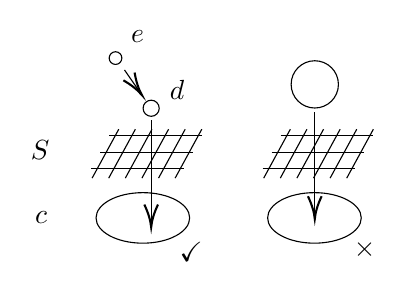
\begin{tikzpicture}[x=0.75pt,y=0.75pt,yscale=-1,xscale=1]
%uncomment if require: \path (0,300); %set diagram left start at 0, and has height of 300

%Shape: Ellipse [id:dp10401378338786049] 
\draw   (74,113.39) .. controls (74,106.67) and (84.1,101.22) .. (96.56,101.22) .. controls (109.01,101.22) and (119.11,106.67) .. (119.11,113.39) .. controls (119.11,120.11) and (109.01,125.56) .. (96.56,125.56) .. controls (84.1,125.56) and (74,120.11) .. (74,113.39) -- cycle ;
%Shape: Grid [id:dp09583060841478219] 
\draw  [draw opacity=0] (81.95,70.67) -- (126.56,70.67) -- (113.72,94.22) -- (69.11,94.22) -- cycle ; \draw   (84.95,70.67) -- (72.11,94.22)(92.95,70.67) -- (80.11,94.22)(100.95,70.67) -- (88.11,94.22)(108.95,70.67) -- (96.11,94.22)(116.95,70.67) -- (104.11,94.22)(124.95,70.67) -- (112.11,94.22) ; \draw   (80.31,73.67) -- (124.92,73.67)(75.95,81.67) -- (120.56,81.67)(71.59,89.67) -- (116.2,89.67) ; \draw    ;
%Shape: Circle [id:dp31189924819685966] 
\draw   (80.33,36.39) .. controls (80.33,34.7) and (81.7,33.33) .. (83.39,33.33) .. controls (85.08,33.33) and (86.44,34.7) .. (86.44,36.39) .. controls (86.44,38.08) and (85.08,39.44) .. (83.39,39.44) .. controls (81.7,39.44) and (80.33,38.08) .. (80.33,36.39) -- cycle ;
%Straight Lines [id:da12935033787340267] 
\draw    (87.72,42.11) -- (94.97,52.58) ;
\draw [shift={(96.11,54.22)}, rotate = 235.29] [color={rgb, 255:red, 0; green, 0; blue, 0 }  ][line width=0.75]    (10.93,-3.29) .. controls (6.95,-1.4) and (3.31,-0.3) .. (0,0) .. controls (3.31,0.3) and (6.95,1.4) .. (10.93,3.29)   ;
%Shape: Circle [id:dp7222065551952845] 
\draw   (96.67,60.56) .. controls (96.67,58.41) and (98.41,56.67) .. (100.56,56.67) .. controls (102.7,56.67) and (104.44,58.41) .. (104.44,60.56) .. controls (104.44,62.7) and (102.7,64.44) .. (100.56,64.44) .. controls (98.41,64.44) and (96.67,62.7) .. (96.67,60.56) -- cycle ;
%Straight Lines [id:da7276461675375434] 
\draw    (100.56,66.44) -- (100.56,115.89) ;
\draw [shift={(100.56,117.89)}, rotate = 270] [color={rgb, 255:red, 0; green, 0; blue, 0 }  ][line width=0.75]    (10.93,-3.29) .. controls (6.95,-1.4) and (3.31,-0.3) .. (0,0) .. controls (3.31,0.3) and (6.95,1.4) .. (10.93,3.29)   ;
%Shape: Ellipse [id:dp12697611260252684] 
\draw   (156.67,113.39) .. controls (156.67,106.67) and (166.77,101.22) .. (179.22,101.22) .. controls (191.68,101.22) and (201.78,106.67) .. (201.78,113.39) .. controls (201.78,120.11) and (191.68,125.56) .. (179.22,125.56) .. controls (166.77,125.56) and (156.67,120.11) .. (156.67,113.39) -- cycle ;
%Shape: Grid [id:dp9936460967678797] 
\draw  [draw opacity=0] (164.61,70.67) -- (209.22,70.67) -- (196.39,94.22) -- (151.78,94.22) -- cycle ; \draw   (167.61,70.67) -- (154.78,94.22)(175.61,70.67) -- (162.78,94.22)(183.61,70.67) -- (170.78,94.22)(191.61,70.67) -- (178.78,94.22)(199.61,70.67) -- (186.78,94.22)(207.61,70.67) -- (194.78,94.22) ; \draw   (162.98,73.67) -- (207.59,73.67)(158.62,81.67) -- (203.23,81.67)(154.26,89.67) -- (198.87,89.67) ; \draw    ;
%Shape: Circle [id:dp838751100400853] 
\draw   (168,49.06) .. controls (168,42.77) and (173.1,37.67) .. (179.39,37.67) .. controls (185.68,37.67) and (190.78,42.77) .. (190.78,49.06) .. controls (190.78,55.35) and (185.68,60.44) .. (179.39,60.44) .. controls (173.1,60.44) and (168,55.35) .. (168,49.06) -- cycle ;
%Straight Lines [id:da5932706956135338] 
\draw    (179.39,62.44) -- (179.39,111.89) ;
\draw [shift={(179.39,113.89)}, rotate = 270] [color={rgb, 255:red, 0; green, 0; blue, 0 }  ][line width=0.75]    (10.93,-3.29) .. controls (6.95,-1.4) and (3.31,-0.3) .. (0,0) .. controls (3.31,0.3) and (6.95,1.4) .. (10.93,3.29)   ;

% Text Node
\draw (43.33,109) node [anchor=north west][inner sep=0.75pt]   [align=left] {$\displaystyle c$};
% Text Node
\draw (41.33,75) node [anchor=north west][inner sep=0.75pt]   [align=left] {$\displaystyle S$};
% Text Node
\draw (113,123.67) node [anchor=north west][inner sep=0.75pt]   [align=left] {$\displaystyle \checkmark$};
% Text Node
\draw (197,123) node [anchor=north west][inner sep=0.75pt]   [align=left] {$\displaystyle \times $};
% Text Node
\draw (108.33,46) node [anchor=north west][inner sep=0.75pt]   [align=left] {$\displaystyle d$};
% Text Node
\draw (89.67,22) node [anchor=north west][inner sep=0.75pt]   [align=left] {$\displaystyle e$};


\end{tikzpicture}
    \end{center}

    % 这里, 我们认为指向 $c$ 的态射越复合就越小. 回忆环是一个对象的 $\mathsf {Ab}$-充实范畴, 那么其中的筛正是环的右理想; 筛的大小观念类似于 $p$-进度量下的整数越乘越小.

    一个筛越细, 能 ``通过'' 它的东西就越少, 这解释了\emph{细化}的含义; 反之, 所有东西都能通过的筛就是最粗的筛.
\end{remark}

\begin{example}
	[label={sieve-in-poset}]
	{(偏序集中的筛)}
	对于偏序集 $P$ 的元素 $p$, 记 $\downarrow p = \{x\in P\mid x\leq p\}$. 那么 $p$ 上的一个筛 $S$ 即是 $\downarrow p$ 的子集, 使得若 $x\in S$, $y\leq x$, 则 $y\in S$. 称这样的 $S$ 为 $\downarrow p$ 的\emph{向下封闭子集}.
\end{example}

\begin{example}
	[label={sieve-from-cover}]
	{(覆盖产生筛)}
	设 $X$ 为拓扑空间, $\{U_i\}$ 是其中开集 $V$ 的一个开覆盖. 那么
	$$
	\big\{W\subset V \mid \exists i, W \subset U_i\big\}
	$$
	构成 $\operatorname{Open}(X)$ 中 $V$ 上的一个筛. 直观上每个 $U_i$ 是筛上的一个 ``洞'', 比它小的对象能 ``通过'' 这个筛.
\end{example}

\begin{prop}
	[label={sieve-and-subfunctor}]
    {(筛与子函子)}
    范畴 $\mathcal C$ 的对象 $c$ 上的筛自然地一一对应于 $\yo(c)$ 的子函子.
\end{prop}

\begin{proof}
    设 $S$ 是 $c$ 上的筛, 那么
    $$
    X\colon \mathcal C^{\op}\to\mathsf {Set},\,X(d) := \{f\colon d\to c \mid f\in S\} \subset \operatorname{Hom}_{\mathcal C}(d,c) = \yo(c)(d)
    $$
    构成 $\yo(c)$ 的子函子.
    设 $X \to \yo(c)$ 为子函子, 那么
    $$
    S:=\big\{
        f \colon d\to c \mid f\in X(d)
    \big\}
    $$
    是 $c$ 上的筛. 很明显, 这两个对应是互逆的.
    注意 $X$ 的函子性恰好等价于筛 $S$ 为右理想.
    容易验证筛 $S$ 沿态射 $f\colon d\to c$ 的拉回等同于 $\yo(c)$ 的子对象 $X$ 沿 $f\colon \yo(d)\to \yo(c)$ 的拉回.
\end{proof}

在后文中, 我们将自由地运用上述对应, 将 $c$ 上的筛与 $\yo(c)$ 的子函子完全等同, 请读者务必熟悉.

%\begin{remark}
%    {}
%    若将 $\widehat {\mathcal C}$ 的对象称作 $\mathcal C$ 的 ``广义对象'', 那么 $\yo(c)$ 的子函子可称作 $c$ 的 ``广义子对象''.
%
%    $\mathcal C$ 的 ``广义对象'' $X$ 的子对象, 根据命题 \ref{subfunctor-description} 的描述, 也可视为 $X$ 上的 ``筛''.
%\end{remark}

\begin{example}
	[label={principal-sieve}]
	{(主筛)}
	对于范畴 $\mathcal C$ 中的态射 $f\colon c'\to c$,
	所有穿过 $f$ 的态射 $c''\to c'\overset{f}{\to} c$ 构成 $c$ 上的一个筛 $\downarrow f$, 称为\emph{主筛} (principal sieve).
	这类似于环的主理想.
	$\downarrow f$ 对应的 $\yo(c)$ 的子函子恰为 $\yo(f)\colon \yo(c') \to \yo(c)$ 的像.
\end{example}

\begin{example}
	[label={sieve-from-cover-subfunctor}]
	{(覆盖产生的筛对应的子函子)}
	继续例 \ref{sieve-from-cover}, 设 $S$ 为覆盖 $\{U_i\}$ 生成的筛 (视为 $\yo(V)$ 的子函子), 那么下图是余等化子.
	\begin{equation}
		\label{sieve-coeq}
		\begin{tikzcd}[ampersand replacement=\&]
			{\coprod_{i,j}\yo(U_i\cap U_j)} \& {\coprod_i \yo(U_i)} \& S
			\arrow[shift right, from=1-1, to=1-2]
			\arrow[shift left, from=1-1, to=1-2]
			\arrow[from=1-2, to=1-3]
		\end{tikzcd}
	\end{equation}
	这是因为, 由 $S$ 的定义, 对 $W\in\operatorname{Open}(X)$, 若存在 $i$, $W\subset U_i$, 则 $S(W)$ 是单元集; 否则 $S(W)$ 是空集. 由此可知下图是集合范畴中的余等化子.
	\[\begin{tikzcd}[ampersand replacement=\&, column sep=small]
		{\coprod_{i,j}\operatorname{Hom}_{\operatorname{Open}(X)}(W,U_i\cap U_j)} \& {\coprod_i \operatorname{Hom}_{\operatorname{Open}(X)}(W,U_i)} \& {S(W)}
		\arrow[shift right, from=1-1, to=1-2]
		\arrow[shift left, from=1-1, to=1-2]
		\arrow[from=1-2, to=1-3]
	\end{tikzcd}\]
	而预层的余极限是 ``逐点'' 的, 于是得 (\ref{sieve-coeq}).
	
	对 $X$ 上的任意预层 $F$, 以 $\operatorname{Hom}_{\operatorname{Presh}(X)}(-,F)$ 作用于 (\ref{sieve-coeq}), 可知下图是集合范畴中的等化子.
	\begin{equation}
		\begin{tikzcd}[ampersand replacement=\&]
			{\operatorname{Hom}_{\operatorname{Presh}(X)}(S,F)} \& {\prod_i F(U_i)} \& {\prod_{i,j}F(U_i\cap U_j)}
			\arrow[shift left, from=1-2, to=1-3]
			\arrow[shift right, from=1-2, to=1-3]
			\arrow[from=1-1, to=1-2]
		\end{tikzcd}
		\label{sieve-subfunctor-equalizer}
	\end{equation}
	因此态射集合 $\operatorname{Hom}_{\operatorname{Presh}(X)}(S,F)$ 表达了预层 $F$ 关于覆盖 $\{U_i\}$ 的下降资料 (descent data), 由覆盖 $\{U_i\}$ ``下降'' 到 $V$. 若 $F$ 为层, 就应该有 $$\operatorname{Hom}_{\operatorname{Presh}(X)}(S,F) \simeq F(V) \simeq \operatorname{Hom}_{\operatorname{Presh}(X)}(\yo(V),F).$$
\end{example}

\begin{example}
	[label={maximal-sieve}]
    {(极大筛)}
    所有指向 $c$ 的箭头的集合称为\emph{极大筛}, 也即最粗的筛.
    它对应 $\yo(c)$ 的子对象 $\yo(c)$ 自身.
    注意, $c$ 上的一个筛是极大筛当且仅当它包含 $\operatorname{id}_c$.
    设 $S$ 是 $c$ 上的筛, $f\colon d\to c$, 那么 $f\in S$ 当且仅当 $f^*S$ 为 $d$ 上的极大筛.
\end{example}

\subsubsection{预层范畴的子对象分类子}

假设 $\widehat{\mathcal C}$ 中存在子对象分类子 $\Omega$, 那么 $\Omega$ 是确定的: 由米田引理, 有自然同构
$$
\Omega(c) \simeq \operatorname{Hom}_{\widehat {\mathcal C}}(\yo(c),\Omega)
\simeq \operatorname{Sub}_{\widehat {\mathcal C}}(\yo(c))\simeq \{\text{$c$ 上的筛}\}.
$$
下面证明这个预层确实是 $\widehat{\mathcal C}$ 的子对象分类子.

\begin{prop}
	[label={presheaf-category-subobject-classifier}]
	{(预层范畴的子对象分类子)}
	在任意范畴 $\mathcal C$ 上, 定义预层 $\Omega\colon \mathcal C^{\op}\to\mathsf {Set}$, $\Omega(c) := \{\text{$c$ 上的筛}\}$, 且对态射 $f\colon d\to c$, $\Omega(f)\colon \Omega(c)\to \Omega(d)$ 为筛的拉回. 那么 $\Omega$ 是 $\widehat{\mathcal C}$ 的子对象分类子.
\end{prop}

\begin{proof}
    定义态射 $\top\colon 1 \to \Omega,$
    对每个对象 $c$ 选出 $\Omega(c)= \operatorname{Sub}_{\widehat {\mathcal C}}(\yo(c))$
    中的子对象 $\yo(c)$ 自身, 也即 $c$ 上的极大筛.
    设 $Y\to X$ 是 $\widehat{\mathcal C}$ 中的任意子对象.
    定义态射 $\chi \colon X \to \Omega$, 将 $x\in X(c)$ 对应到 $c$ 上的筛
    \begin{equation}
    	\chi_c(x) := \big\{f \colon d \to c \mid X(f)(x) \in Y(d)\big\}.
    	\tag{$\star$}
    \end{equation}
    注意 $\chi_c(x)$ 是极大筛当且仅当 $\operatorname{id}_c \in \chi_c(x)$, 也即 $x \in Y(c)$,
    所以子对象 $Y\to X$ 是如下的拉回.
    % https://q.uiver.app/#q=WzAsNCxbMCwxLCJYIl0sWzEsMSwiXFxPbWVnYSJdLFsxLDAsIjEiXSxbMCwwLCJZIl0sWzMsMF0sWzAsMSwiXFxjaGkiLDJdLFsyLDEsIlxcdG9wIl0sWzMsMl1d
    \[\begin{tikzcd}[ampersand replacement=\&]
    	Y \& 1 \\
    	X \& \Omega
    	\arrow[from=1-1, to=2-1]
    	\arrow["\chi"', from=2-1, to=2-2]
    	\arrow["\top", from=1-2, to=2-2]
    	\arrow[from=1-1, to=1-2]
    \end{tikzcd}\]
	这证明了 $\Omega$ 是 $\widehat{\mathcal C}$ 的子对象分类子, 且 $\top\colon 1\to\Omega$ 是万有子对象.
\end{proof}

\begin{remark}
	[label={presheaf-subobject-classifier-motivation}]
	{(特征函数的定义的解释)}
	假设下图中右侧方块以及长方形为拉回,
	可得左侧方块为拉回,
	% https://q.uiver.app/#q=WzAsNixbMSwwLCJZIl0sWzEsMSwiWCJdLFswLDEsIlxceW8oYykiXSxbMiwwLCIxIl0sWzIsMSwiXFxPbWVnYSJdLFswLDAsIlxcY2hpX2MoeCkiXSxbMyw0LCJcXHRvcCJdLFsxLDQsIlxcY2hpIiwyXSxbMCwzXSxbMCwxXSxbMiwxLCJ4IiwyXSxbNSwyXSxbNSwwXV0=
	\[\begin{tikzcd}[ampersand replacement=\&]
		{\chi_c(x)} \& Y \& 1 \\
		{\yo(c)} \& X \& \Omega
		\arrow["\top", from=1-3, to=2-3]
		\arrow["\chi"', from=2-2, to=2-3]
		\arrow[from=1-2, to=1-3]
		\arrow[from=1-2, to=2-2]
		\arrow["x"', from=2-1, to=2-2]
		\arrow[from=1-1, to=2-1]
		\arrow[from=1-1, to=1-2]
	\end{tikzcd}\]
	因此 $\chi_c(x) = \{f\in\yo(c)(d)\mid x\circ f\in Y(d)\}$.
	注意到对于 $x\in X(c)$, 有 $x\in Y(c)$ 当且仅当上图中存在提升 $\yo(c)\to Y$,
	当且仅当 $\chi_c(x) = \yo(c)$.
	这解释了态射 $\chi\colon X\to\Omega$ 的构造.
\end{remark}

综合上述论证, 我们得到
\begin{prop}{}
    $\widehat {\mathcal C}$ 是一个\topos{}.
\end{prop}

\begin{example}
	[label={G-set-topos}]
    {($G$-集)}
    例 \ref{G-set-presheaf-category} 介绍了 $G$-集范畴, 即 $\mathsf BG$ 上的预层范畴. 由于 $\mathsf BG$ 只有一个对象且态射均为自同构,
    其上仅有两个筛, 空集与极大筛.
    
    因此, $G$-集范畴的子对象分类子 $\Omega$ 是二元集合 $\{\top,\bot\}$, 其上带有 $G$ 的平凡作用.
    事实上, 一个 $G$-集 $X$ 的子对象 $Y$ 是其中 $G$-作用下封闭的子集. 其对应的特征函数 $X\to\{\top,\bot\}$ 就是子集 $Y$ 的特征函数.
\end{example}

%回忆\topos{}中的子对象分类子 $\Omega$ 有内蕴 Heyting 代数结构. 对于预层范畴的情形, 其结构态射可用筛具体写出.

%\begin{prop}
%	{}
%	设 $R,S$ 是范畴 $\mathcal C$ 对象 $c$ 上的筛, 即 $\Omega(c)$ 的元素.
%	\begin{itemize}
%		\item 
%		$R\land S$
%	\end{itemize}
%\end{prop}

\section{景}

\philoquote{Attempting to define a ``Weil cohomology'' with the formal properties 
necessary to establish the Weil conjectures, Grothendieck discovered \'etale 
cohomology, a fusion of ordinary sheaf cohomology and Galois cohomology. The definition required an extension of the concept of sheaf to the idea 
of a sheaf on a site --- a category equipped with an a priori notion of covering.}{Andr\'e Joyal, Myles Tierney, \cite{EGG}}

Grothendieck 意识到, 层的概念所需的关键信息是一个对象 $U$ 何时被一族进入 $U$ 的态射 (甚至不一定是 $U$ 的子对象) 所\emph{覆盖}.

\subsection{从覆盖到 Grothendieck 拓扑}

本小节有许多的定义, 在读者看来这些定义可能有些冗余. 这或许是历史的遗留, 但每个定义有各自的长处.

\begin{definition}{(覆盖结构)}
    范畴 $\mathcal C$ 上的一个\emph{覆盖结构} (coverage) $T$ 是如下资料: 对每个对象 $c$ 指定一个集合 $T(c)$, 其元素为态射族 $\{f_i \colon c_i \to c\}_{i\in I}$, 称为 $c$ 的 $T$-\emph{覆盖族} (covering family), 满足
    \begin{itemize}
    	\item (拉回下的稳定性) 若 $\{f_i \colon c_i \to c\}_{i\in I}\in T(c)$, 对任意态射 $g \colon d \to c$,
    	存在 $\{h_j \colon d_j \to d\}_{j\in J}\in T(d)$
    	使得每个 $gh_j$ 都穿过某个 $f_i$.
    \end{itemize}
	
    %带有覆盖结构的范畴 $(\mathcal C,T)$ 称为\emph{景} (site).
    对于两个覆盖结构 $T,T'$, 若 $T\subset T'$, 则称 $T'$ 较\emph{细} (fine).
\end{definition}

\begin{remark}
	{(具有拉回的范畴上的覆盖结构)}
	对于具有拉回的范畴 $\mathcal C$, 我们通常要求覆盖结构满足如下更强的条件.
	\begin{itemize}
		\item (拉回下的稳定性) 若 $\{f_i \colon c_i \to c\}_{i\in I}\in T(c)$, $g \colon d \to c$,
		则 $\{g^*(f_i) \colon d_i \to d\}_{i\in I}\in T(d)$.
	\end{itemize}
\end{remark}

%对于拓扑空间的开集范畴, 拉回下的稳定性相当于若一族开集覆盖了 $U$, 那么它们也覆盖了 $U$ 的任何子集.

%\begin{remark}{}
%    上面定义的覆盖结构有时也称为范畴上的 \emph{Grothendieck 拓扑}, 但这个词的含义有时要窄一些.
%\end{remark}

\begin{definition}
	[label={sheaf-condition}]
	{(关于态射族的层条件)}
	设 $F$ 是范畴 $\mathcal C$ 上的预层. 设 $M = \{f_i\colon c_i\to c\}_{i\in I}$ 是 $\mathcal C$ 中的一族共终点的态射. 称 $F$ 满足关于 $M$ 的\emph{层条件}, 是指对任意一组相容的元素 $(s_i\in F(c_i))_{i\in I}$,
	存在唯一的 $s\in F(c)$ 满足 $$F(f_i)(s)=s_i\,\forall i\in I.$$
	其中, 一组元素 $(s_i\in F(c_i))_{i\in I}$ \emph{相容}是指对任意态射 $f\colon d \to c_i$, $g\colon d \to c_j$, 有 $$F(f)(s_i) = F(g)(s_j) \in F(d).$$
	
	若将上面的 ``存在唯一'' 改为 ``存在至多一个'', 得到的条件称为\emph{分离性}条件.
	
	在 $\mathcal C$ 具有拉回的条件下, 层条件可简洁地表述为如下等化子,
	% https://q.uiver.app/#q=WzAsMyxbMCwwLCJGKGMpIl0sWzEsMCwiXFxwcm9kX3tpfSBGKGNfaSkiXSxbMiwwLCJcXHByb2Rfe2ksan0gRihjX2lcXHRpbWVzX2MgY19qKSJdLFsxLDIsIiIsMCx7Im9mZnNldCI6LTF9XSxbMSwyLCIiLDIseyJvZmZzZXQiOjF9XSxbMCwxXV0=
	\[\begin{tikzcd}[ampersand replacement=\&]
		{F(c)} \& {\prod_{i} F(c_i)} \& {\prod_{i,j} F(c_i\times_c c_j).}
		\arrow[shift left, from=1-2, to=1-3]
		\arrow[shift right, from=1-2, to=1-3]
		\arrow[from=1-1, to=1-2]
	\end{tikzcd}\]

	
	设 $S\to \yo(c)$ 是 $\{f_i\colon c_i\to c\}_{i\in I}$ 生成的筛对应的子函子 (命题 \ref{sieve-and-subfunctor}), 那么一组相容的元素等同于自然变换 $S\to F$,	从而层条件等价于自然变换 $S\to F$ 唯一地穿过 $\yo(c)$, 也即如下映射是同构.
	$$
	\operatorname{Hom}_{\widehat {\mathcal C}}(\yo(c),F) \to \operatorname{Hom}_{\widehat {\mathcal C}}(S,F)
	$$
	(分离性条件等价于它是单射.) 对比例 \ref{sieve-from-cover-subfunctor} 中的式 (\ref{sieve-subfunctor-equalizer}).
	$F$ 关于 $S$ 的层条件也可表述为 $F$ 是关于 $S\to \yo(c)$ 的\emph{局部对象} (定义 \ref{local-objects}), 这种表述的优势在于能一字不改地推广为 Lawvere--Tierney 拓扑的层条件 (定义 \ref{Lawvere--Tierney-topology-sheaf}).
\end{definition}

\begin{definition}
	{(关于覆盖的层条件)}
	设 $F$ 是范畴 $\mathcal C$ 上的预层. 设 $T$ 是范畴 $\mathcal C$ 上的覆盖结构. 称 $F$ 满足关于 $T$ 的\emph{层条件}就是指 $F$ 满足关于其中每个态射族的层条件.
\end{definition}

\begin{remark}
	{(覆盖结构的粗细)}
	由定义, 覆盖结构越\emph{细}, 对应的层条件就越\emph{强}, 层就越\emph{少}. 注意, 覆盖结构的粗细与筛的粗细是两个不同的概念. 对于覆盖结构 $T\subset T'$, 我们称 $T'$ 较细; 对于筛 $S\subset S'$, 我们称 $S$ 较细 (见注 \ref{sieve-intuition}).
\end{remark}

\begin{definition}
	{(层范畴)}
	设 $T$ 是范畴 $\mathcal C$ 上的覆盖结构. 定义\emph{层范畴} $\operatorname{Sh}(\mathcal C,T)$ 为 $\widehat {\mathcal C}$ 中满足关于 $T$ 的层条件的预层构成的全子范畴.
\end{definition}

``覆盖结构'' 是从 \emph{Grothendieck 拓扑}的概念中分离出的一个比较重要的条件. Grothendieck 拓扑的完整概念如下.

\begin{definition}
	[label={Grothendieck-topology}]
	{(Grothendieck 拓扑)}
	范畴 $\mathcal C$ 上的一个 \emph{Grothendieck 拓扑} (或 Grothendieck 覆盖结构) $J$ 是如下结构: 对每个对象 $c$ 指定一个集合 $J(c)$, 其元素为 $c$ 上的\emph{筛}, 称为\emph{覆盖筛} (covering sieve), 满足
	\begin{enumerate}[(1)]
		\item (极大筛) 任何对象 $c$ 上的极大筛 (定义 \ref{maximal-sieve}) 属于 $J(c)$;
		\item (拉回下的稳定性) 若 $S\in J(c)$, $f \colon d \to c$,
		则 $f^*S\in J(d)$.
		\item (传递性) 若 $S\in J(c)$, $R$ 是 $c$ 上的另一个筛, 使得对任意 $(f\colon d\to c)\in S$, 都有 $f^*R\in J(d)$, 那么 $R\in J(c)$.
	\end{enumerate}
\end{definition}

注意由定义可得对 $c$ 上的两个筛 $S\subset R$, 若 $S\in J(c)$, 则 $R\in J(c)$.
此外, 两个覆盖筛的交仍是覆盖筛.

\begin{propdef}
	[label={sieve-cover-arrow}]
	{(筛对态射的覆盖, Grothendieck 拓扑的等价条件)}
	固定范畴 $\mathcal C$ 上的 Grothendieck 拓扑 $J$, 我们称一个对象 $c$ 上的筛 $S$ \emph{覆盖}态射 $f\colon d\to c$ 是指 $f^*S\in J(d)$.
	例如 $S$ 覆盖 $\operatorname{id}_c$ 就是说 $S$ 覆盖 $c$.
	此时 Grothendieck 拓扑的条件等价于如下的形式.
	\begin{enumerate}[(1')]
		\item 筛 $S$ 覆盖它的所有元素;
		\item 若 $S$ 覆盖 $f$, 则 $S$ 也覆盖 $fg$ (只要 $f,g$ 可复合);
		\item (传递性) 若 $S$ 覆盖 $f$, $R$ 覆盖 $S$ 的每个元素, 则 $R$ 覆盖 $f$.
	\end{enumerate}
\end{propdef}

\begin{proof}
	~
	\begin{itemize}
		\item $\text{(1)(2)(3)} \Rightarrow \text{(1')(2')(3')}$.
		(1')(2') 是直接的; 只有 (3') 需要稍微说明.
		假设 $S$ 覆盖 $f\colon d\to c$ (即 $f^*S\in J(d)$) 且 $R$ 覆盖 $S$ 的每个元素. 对任意 $g\in f^*S$, 有 $fg\in S$, 从而 $R$ 覆盖 $fg$, $f^*R$ 覆盖 $g$.
		由 (3), $f^*R\in J(d)$.
		\item $\text{(1')(2')(3')} \Rightarrow \text{(1)(2)(3)}$. 只需要考虑 $\operatorname{id}_c$ 即可.
	\end{itemize}
\end{proof}

对于拓扑空间的开集范畴, ``极大筛是覆盖'' 相当于任何开集 $U$ 都覆盖了自己; 传递性相当于若一族开集覆盖了 $U$ 的每个局部, 那么它们也覆盖了 $U$.

%筛 $S$ 覆盖态射 $f\colon d\to c$ 在直观上说的是 $S$ 覆盖了 $f$ 的像 (不一定是范畴论意义下的像).

\begin{remark}
	[label={saturation-condition-covering}]
	{(关于饱和性条件)}
	Grothendieck 拓扑的定义中, 要求覆盖族是筛且满足\emph{极大筛}和\emph{传递性}的条件, 这些都是\emph{饱和性条件} (saturation condition), 假设一个覆盖结构不满足这些条件, 我们也可以关于这些条件取 ``闭包'' 而不影响层条件:
	\begin{itemize}
		\item (筛) 一族态射 $M= \{f_i\colon c_i \to c\}_{i\in I}$ 的层条件等价于其生成的筛的层条件;
		\item (极大筛) 极大筛的层条件是平凡的 (一族态射只要包含了 $\operatorname{id}_c$, 其层条件就是平凡的);
		\item (传递性) 若预层 $F$ 满足 $\{f_i\colon c_i\to c\}_{i\in I}$ 的层条件, 且对每个 $i$ 都有一族态射 $\{h_{ij}\colon c_{ij}\to c_i\}_{j\in I_i}$ 使得 $F$ 满足其层条件, 那么 $F$ 也满足复合态射族 $\{f_i\circ h_{ij}\colon c_{ij}\to c\}_{i\in I,j\in I_i}$ 的层条件. (见 Elephant \cite{Elephant} C2.1 节引理 7.)
	\end{itemize}
	因此在 Grothendieck 拓扑的定义中只有\emph{拉回下的稳定性}是关键的.
\end{remark}

\begin{prop}
	[label={sieve-and-sheaf-condition}]
	{(筛与层条件的关系)}
	\begin{enumerate}[(1)]
		\item 设 $R, S$ 是 $c$ 上的筛. 若预层 $F$ 满足关于 $R$ 的层条件, 且 $R\subset S$, 则 $F$ 也满足关于 $S$ 的层条件.
		\item 设 $R, S$ 是 $c$ 上的筛. 若预层 $F$ 满足关于 $R$ 的层条件, 且对任意 $f\in R$, $F$ 满足关于 $f^*S$ 的层条件, 则 $F$ 也满足关于 $S$ 的层条件.\label{sieve-transitive-sheaf-condition}
	\end{enumerate}
\end{prop}
\begin{proof}
	~
	\begin{enumerate}
		[(1)]
		\item 任意态射 $S\to F$ 复合 $R\hookrightarrow S$ 得到 $R\to F$, 从而唯一地延拓为 $\yo(c) \to F$.
		\item 考虑集合 $S'= \{fh\mid f\in R, h\in f^*S\}$. 由注 \ref{saturation-condition-covering} 中关于传递性的讨论, $F$ 满足关于 $S'$ 的层条件. 而 $S'\subset S$, 故 $S'$ 生成的筛包含于 $S$; 由 (1), $F$ 满足关于 $S$ 的层条件.
	\end{enumerate}
\end{proof}

\begin{prop}
	[label={finest-topology-sheaf}]
	{}
	设 $F$ 是范畴 $\mathcal C$ 上的预层, 则 $\mathcal C$ 上存在一个最细的 Grothendieck 拓扑 $J_F$ 使得 $F$ 满足关于 $J_F$ 的层条件.
\end{prop}
\begin{proof}
	定义覆盖结构 $J_F$ 如下,
	$$
	J_F(c) = \{\text{$c$ 上的筛 $S\hookrightarrow\yo(c)$} \mid \text{对任意 $f\colon d\to c$, $F$ 满足关于 $f^*S$ 的层条件}\}.
	$$
	由定义, 对任意 Grothendieck 拓扑 $J$, 若 $F$ 为 $J$-层, 则 (由 $J$-覆盖筛的拉回稳定性) $J\subset J_F$.
	我们只需验证 $J_F$ 为 Grothendieck 拓扑.
	\begin{itemize}
		\item (极大筛) 极大筛的拉回仍是极大筛, 极大筛的层条件是平凡的, 故极大筛均属于 $J_F$.
		\item (拉回下的稳定性) 假设 $S\in J_F(c)$, $f\colon d\to c$, 由于 $f^*S$ 的拉回也是 $S$ 的拉回, 故 $f^*S\in J_F(d)$.
		\item (传递性)
		假设 $S\in J_F(c)$,
		且 $R$ 是 $c$ 上的另一个筛,
		使得对任意 $(f\colon d\to c)\in S$, $f^*R\in J_F(d)$.
		%
		%		那么对任意 $h\colon d\to c$,
		%			$F$ 满足关于 $f^*S$ 的层条件,
		%			且对任意 $g\colon e\to d$,
		%			$F$ 满足关于 $g^*f^*R$ 的层条件.
		%
		%由注 \ref{saturation-condition-covering} 关于传递性的讨论,
		%
		
		由 $S\in J_F(c)$, 对任意 $h\colon b\to c$,
		$F$ 满足 $h^*S$ 的层条件.
		
		对任意 $(k\colon a\to b)\in h^*S$, $(hk\colon a\to c)\in S$.
		由 $R$ 的假设, $(hk)^*R = k^*h^*R\in J_F(a)$; 特别地, $F$ 满足关于 $k^*h^*R$ 的层条件.
		
		由以上结论及命题 \ref{sieve-and-sheaf-condition} (\ref{sieve-transitive-sheaf-condition}),
		$F$ 满足关于 $h^*R$ 的层条件.
		%
		这说明 $R\in J_F(c)$.
	\end{itemize}
\end{proof}

\begin{prop}
	[label={coverage-generated-Grothendieck-topology}]
	{(覆盖与 Grothendieck 拓扑的关系)}
	设范畴 $\mathcal C$ 上有覆盖结构 $T$. 那么存在 Grothendieck 拓扑 $J$ 给出与 $T$ 相同的层条件.
%	具体地,
%	$$
%	J(c)=\{\text{$c$ 上的筛 $S$} \mid \cdots\}.
%	$$
%	\todo{}
\end{prop}
\begin{proof}
	令 $\overline{T}$ 为 $T$ 中的覆盖族生成的筛的集合, 
	则 $T$ 的层条件等价于 $\overline{T}$ 的层条件.
	令 $J$ 为所有包含 $\overline{T}$ 的 Grothendieck 拓扑的交, 则 $J$ 为 Grothendieck 拓扑. ($J$ 的表达式可显式写出, 此处略去.)
	设 $F$ 为 $T$-层. 由命题 \ref{finest-topology-sheaf} 的证明, $\overline{T}\subset J_F$, 从而 $J\subset J_F$.
	这说明 $F$ 为 $J$-层. 故 $J$ 给出与 $T$ 相同的层条件.
	%\todo{}sieve-and-sheaf-condition
\end{proof}

\begin{remark}
	{}
	一般而言, 即使覆盖结构很简洁, 也难以根据命题 \ref{coverage-generated-Grothendieck-topology} 具体写出对应的 Grothendieck 拓扑. 覆盖结构与 Grothendieck 拓扑的关系正如一个群的生成元和群本身的关系.
\end{remark}

下面这个概念也被某些文献用作 Grothendieck 拓扑的定义.

\begin{definition}
	{(Grothendieck 拓扑基)}
	设范畴 $\mathcal C$ 有拉回. 其上的一组 \emph{Grothendieck 拓扑基} (basis for a Grothendieck topology, 又称 \emph{Grothendieck 预拓扑}, pretopology) $K$ 是如下结构:
	对每个对象 $c$ 指定一个集合 $K(c)$, 其元素为态射族 $\{f_i\colon c_i\to c\}_{i\in I}$, 满足
	\begin{itemize}
		\item (恒等) $\{\operatorname{id}_c\} \in K(c)$;
		\item (拉回下的稳定性) 若 $\{f_i\colon c_i\to c\}_{i\in I} \in K(c)$, $g\colon d\to c$, 则 $\{g^*f_i\}_{i\in I}\in K(d)$;
		\item (传递性) 若 $\{f_i\colon c_i\to c\}_{i\in I} \in K(c)$, 且对每个 $i\in I$, 有 $\{g_{ij}\colon d_{ij}\to c_i\}_{j\in I_i} \in K(c_i)$, 则 $\{f_i\circ g_{ij}\colon d_{ij}\to c\}_{i\in I,j\in I_i} \in K(c)$.
	\end{itemize}
\end{definition}

\begin{definition}
	{(基生成的 Grothendieck 拓扑)}
	Grothendieck 拓扑基 $K$ \emph{生成}的 Grothendieck 拓扑 $J$ 如下:
	$$
	J(c) = \{ \text{$c$ 上的筛 $S$} \mid \exists R\in K(c), R\subset S \}.
	$$
	为了表达的方便, 我们也将用覆盖结构或 Grothendieck 拓扑基来代指其生成的 Grothendieck 拓扑.
\end{definition}

%\begin{remark}
%	{}
%	引入\emph{覆盖结构}以及 \emph{Grothendieck 拓扑基}等概念的目的大约是
%	\begin{itemize}
%		\item 方便给出 Grothendieck 拓扑 (不需要给出所有的筛);
%		\item 方便验证层条件 (不需要对所有的筛验证).
%	\end{itemize}
%%	而 Grothendieck 拓扑的优势在于
%%	\begin{itemize}
%%		\item 唯一性 (命题 \ref{coverage-generated-Grothendieck-topology});
%%		\item 与后文介绍的 Lawvere--Tierney 拓扑 (定义 \ref{Lawvere--Tierney-topology}) 的关系.
%%	\end{itemize}
%	\emph{覆盖结构}与 Grothendieck 拓扑的关系正如一个群的生成元和群本身的关系.
%\end{remark}

\begin{definition}
	[label={site-definition}]
	{(景)}
	带有 Grothendieck 拓扑的 (小) 范畴称为\emph{景}.
\end{definition}

\begin{definition}
	[label={convention-coverage}]
	{(Grothendieck 拓扑语境下的 ``覆盖'')}
	当范畴 $\mathcal C$ 上有 Grothendieck 拓扑 $J$ 时, 作如下约定: 称一族态射 $\{f_i\colon c_i\to c\}$ \emph{覆盖}了对象 $c$ 是指其生成的筛 $$\{h\colon d\to c\mid \text{$h$ 穿过某个 $f_i$}\}$$ 是 $J$-覆盖筛.
\end{definition}

\begin{remark}
	{(关于景的小性)}
	我们一般要求景是小的, 但是许多结论可以推广到所谓\emph{本质小}的景, 即其有一个小的 $J$-稠密子范畴 (定义 \ref{site-J-dense-subcategory}).
\end{remark}



\subsection{常见的景}

% 正如环中一族元素可以生成一个右理想, 范畴 $\mathcal C$ 中一族指向 $U$ 的箭头也可以生成一个筛. 容易看到, 将覆盖族替换为生成的筛, 不影响层的概念 (正如将环中的一族元素替换为其生成的理想, 不影响对应谱上的闭集一样). 因此我们不妨考虑仅由筛构成的覆盖结构.

\begin{example}
	{}
	每个范畴 $\mathcal C$ 都构成一个平凡的景, 其上的覆盖结构为空.
	该覆盖结构对应的 Grothendieck 拓扑称为\emph{平凡拓扑} $J_{\text{平凡}}$, 其中仅包含每个对象上的极大筛.
	一族态射 $\{f_i\colon c_i\to c\}$ 覆盖 $c$ 当且仅当某个 $f_i$ 穿过 $\operatorname{id}_c$, 即 $f_i$ 为收缩.
	由定义, 这个景上的层是 $\mathcal C$ 上的预层.
\end{example}

\begin{example}
    [label={topological-space-as-site}]
    {(拓扑空间)}
    拓扑空间 $X$ 的开集范畴 $\operatorname{Open}(X)$ 构成一个景, 其上的覆盖结构是\emph{开覆盖}.
    注意此时 ``拉回下的稳定性'' 即是说若一族开集 $\{U_i\}$ 覆盖了 $V$, 那么对于 $W\subset V$, $\{U_i\land W\}$ 覆盖了 $W$.
    %因为每个可表函子 $\yo(U)$ 都是层, 所以这个覆盖结构定义的 Grothendieck 拓扑是次典范的.
\end{example}

%\todo{解释景的小性}

\begin{example}
    {(拓扑空间范畴)}
    拓扑空间的范畴\footnotemark{}上有一个由\emph{开覆盖}确定的覆盖结构.
\end{example}

\footnotetext{$\mathsf {Top}$ 不是小范畴, 因为每个集合都能配上离散拓扑成为一个拓扑空间. 但是出于实用的目的, 我们可以考虑其中小的子范畴, 如可分 Hausdorff 空间范畴 (回忆, 可分空间是指有可数稠密子集的空间).}

\begin{example}
	[label={locale-as-site}]
    {(位象)}
    % 定义\emph{位象}是一个偏序集 $A$, 存在有限交与任意并 (若将偏序集视为范畴, 这个条件就是说存在有限极限与任意余极限), 且满足分配律
    % $$a \wedge \bigvee_{i\in I} b_i = \bigvee_{i\in I} (a\wedge b_i)\,(\forall a,b_i\in A),$$
    % 其中 $I$ 是任意集合.
    % 位象的态射 $A\to B$ 是偏序集的\emph{反向}态射 $B\to A$ (想象开集的拉回), 保持有限交与任意并.
    
    对于\fm{} $A$, 将其视为范畴, 我们定义 $A$ 上的覆盖结构:
    当一族态射 $\{U_i \to U\}_{i\in I}$ 满足 $U = \bigvee_{i\in I} U_i$ 时, 称其为覆盖族.
    由此, 每个位象都 (反变地) 对应一个景.
\end{example}

\begin{example}
    [label={cartsp-site}]
    {(Cartesius 空间)}
    考虑 Cartesius 空间\footnotemark{}的范畴 $\mathsf {CartSp}$, 其中的对象为 $\mathbb{R}^0,\mathbb{R}^1,\mathbb{R}^2,\cdots$,
    态射为光滑映射.
    称 $\mathbb{R}^n$ 的开覆盖 $\{U_i\}$ 为 \emph{好覆盖} (good cover) 是指 $U_i$ 同胚于 $\mathbb{R}^n$, 且任意有限个 $U_i$ 的交 (假若非空) 都同胚于 $\mathbb{R}^n$.
    这给出了 $\mathsf {CartSp}$ 上的一个覆盖结构, 称之为 \emph{Cartesius 空间景}.
    Cartesius 空间景上的层称作\emph{光滑空间} (smooth space), 记 $\mathsf {SmoothSp}$ 为光滑空间的范畴.
    
    记 $\mathsf {Man}$ 为 (光滑) 流形的范畴. 光滑空间是光滑流形的推广: 对于流形 $M$, 定义光滑空间 $$\underline{M}\colon \mathsf {CartSp}^\op\to\mathsf {Set},\ \mathbb{R}^n\mapsto \operatorname{Hom}_{\mathsf {Man}}(\mathbb{R}^n,M),$$
    这给出了嵌入 $\mathsf {Man}\to \mathsf {SmoothSp}$.
    光滑空间是\emph{广义微分几何} (diffeology) 的研究对象. 在量子场论中, 由于人们常常需要考虑 ``场的空间'' (例如两个流形之间的映射的空间), 操作其上的微分形式, 而它们不是传统意义上的流形, 故使用光滑空间的概念能够更清晰地显示几何意义. 参见 Fr\'ed\'eric Paugam \cite{MQF} 第 3 章.
    
    对于光滑空间 $X\colon \mathsf {CartSp}^\op\to\mathsf {Set}$, $X(\mathbb{R}^n)$ 是 ``$\mathbb{R}^n$ 到 $X$ 的光滑映射的集合'' (这不过是米田引理), 也即空间 $X$ 上 $n$ 维 ``广义坐标系'' 的集合. 层条件表示的是 ``广义坐标系'' 的\emph{粘合条件}, 即当 $\mathbb{R}^n=\bigcup U_i$ 为好覆盖时, 一族相容的广义坐标系 $U_i\to X$ 可粘合为广义坐标系 $\mathbb{R}^n\to X$.
    
    一个重要的光滑空间是 ``微分形式的模空间'' $\Omega^k$, 它作为 $\mathsf {CartSp}$ 上的预层将 $\mathbb{R}^n$ 对应到其上 $k$-形式的集合 $\Omega^k(\mathbb{R}^n)$. 称其为微分形式的模空间是因为, 对任意流形 $M$ 有自然同构
    \[\operatorname{Hom}_{\mathsf {SmoothSp}}(\underline{M},\Omega^k) \simeq \Omega^k(M).\]
    容易验证 $\Omega^k$ 满足层条件, 即对于 $\mathbb{R}^n$ 的好覆盖 $\{U_i\}$, 每个 $U_i$ 上相容的微分形式可以给出 $\mathbb{R}^n$ 整体上的微分形式.
\end{example}

\footnotetext{注. Cartesius 是法国数学家 Ren\'e Descartes (``笛卡尔'') 的姓氏的拉丁化写法. %这里的 $\mathbb{R}^n$ 起到的作用正合 Descartes 的原意, 即给出空间的一部分上的坐标.
}

\begin{example}
	{(超几何)}
	$\mathbb{Z}/2\mathbb{Z}$-分次向量空间范畴有一个对称幺半范畴结构, 其交换同构 $V\otimes W\to W\otimes V$ 在奇部分的作用为 $v\otimes w\mapsto -w\otimes v$. 关于此对称幺半范畴结构的交换代数称为\emph{超交换代数}\footnotemark{}. 超几何是超交换代数对应的几何, 是一些量子场论 (如超对称场论, 超引力) 使用的语言.
	考虑范畴 $\mathsf {SupCartSp}$ (超 Cartesius 空间), 其对象 $\mathbb{R}^{n|q} = \mathbb{R}^n\times\mathbb{R}^{0|q}$ 是 ``有 $n$ 个偶坐标和 $q$ 个奇坐标'' 的空间 (物理学家所使用的术语), 即超交换代数
	$C^\infty (\mathbb{R}^n)\otimes \wedge^\bullet (\mathbb{R}^q)^*$
	的形式对偶.
	
	定义 $\mathsf {SupCartSp}$ 上的覆盖结构 $\{\iota_i\times\operatorname{id}\colon U_i\times \mathbb{R}^{0|q}\to\mathbb{R}^{n}\times\mathbb{R}^{0|q}\}$, 其中 $\{\iota_i\colon U_i\to\mathbb{R}^n\}$ 构成 $\mathbb{R}^n$ 的好覆盖.
	于是 $\mathsf {SupCartSp}$ 成为一景, 其上的层称作\emph{超光滑空间} (super smooth space).
	Urs Schreiber \cite{HTTP} 介绍了物理中旋量场等结构用超几何语言的表述, 以及其它对象在\topos{}理论中的表述.
\end{example}
\footnotetext{对超几何与量子场论感兴趣的读者可阅读 IAS 的讲义 \cite{QFT}.}

\begin{example}
    [label={zariski-site}]
    {(Zariski 景)}
    %固定环 $k$,
    考虑\emph{有限表现} (finitely presented) 环 (形如 $\mathbb{Z}[x_1,\cdots,x_n]/(f_1,\cdots,f_m)$ 的环) 的范畴 $\mathsf {Ring}_{\text{fp}}$. 这是一个小范畴\footnotemark.
    考虑其对偶范畴 $\mathsf {Ring}_{\text{fp}}^{\op}$, 也即仿射概形的范畴.
    对于环 $A$, 我们记 $\operatorname{Spec} A \in \mathsf {Ring}_{\text{fp}}^{\op}$ 为 $A$ 在对偶范畴中的化身.

    回忆, Zariski 拓扑的标准开集 (但不一定是全部的开集) 形如 $\operatorname{Spec} A_f \to \operatorname{Spec}A$, 也即局部化的环同态 $A \to A_f$. 若 $n$ 个元素 $f_1,\cdots,f_n \in A$ 生成了单位理想 $(1)$ ($f_1,\cdots,f_n$ 构成了 $\operatorname{Spec}A$ 上的 ``单位分解''),
    规定 $\{\operatorname{Spec}A_{f_i} \to \operatorname{Spec}A\}$ 构成覆盖. 这定义了 $\mathsf {Ring}_{\text{fp}}^{\op}$ 上的一个覆盖结构, 这便是 \emph{Zariski 景}.
    Zariski 景可以提供\emph{综合代数几何} (synthetic algebraic geometry) 的模型
%
    %Zariski 景上的\emph{结构层} (structure sheaf) 是遗忘函子 $\mathsf{Ring}_{\text{fp}} \to \mathsf{Set}$.
    %\todo{这个层的意义}
    %这个层与综合微分几何中的 ``直线'' 有关
    (见定义 \ref{SDG-algebraic-model}; 关于综合代数几何, 见 \cite{FSAG}).
\end{example}

\footnotetext{严格地说, 它是本质小 (essentially small) 范畴, 也即它的对象模掉同构之后构成一个集合.}

\begin{example}
	[label={small-etale-site}]
	{(平展景)}
	{\small (本例需要一些背景知识.)} 平展景是 ``拓扑空间上开集范畴'' 在代数几何中的类比. 设 $X$ 为概形, 考虑概形范畴的俯范畴 $\mathsf {Sch}_{/X}$ 中由平展映射 $U\to X$ 构成的全子范畴 $\mathsf {Sch}_{/X,\text{\'et}}$. 这称作 $X$ 上的 (小)\emph{平展景} (small \'etale site).
\end{example}

\subsection{典范与次典范拓扑}

%如下定义出自 SGA 4 \cite{SGA4} II.2 节.

\begin{propdef}
	[label={canonical-topology}]
	{(次典范和典范 Grothendieck 拓扑)}
	对于范畴 $\mathcal C$ 上的 Grothendieck 拓扑 $J$, 若以下两个等价条件之一成立, 则称之为\emph{次典范} (subcanonical) Grothendieck 拓扑:
	\begin{itemize}
		\item 对每个 $J$-覆盖筛 $S = \{f_i\colon c_i\to c\}$, 考虑 $c_i$ 之间在 $c$ 上 (也即与 $f_i$ 相容) 的所有映射, $S$ 构成该图上的余极限余锥. 这样的筛又称为\emph{有效满} (effective-epimorphic) 的.
		\item 每个可表函子 $\yo(c)$ 都是层, 也即米田嵌入 $\mathcal C\hookrightarrow\widehat {\mathcal C}$ 穿过 $\operatorname{Sh}(\mathcal C,J)$.
	\end{itemize}
	定义\emph{典范 Grothendieck 拓扑}是最细的次典范 Grothendieck 拓扑. (回忆, 称一个 Grothendieck 拓扑较细是指其中覆盖筛较多).
\end{propdef}
\begin{proof}
	设 $S$ 为 $c$ 上的筛, $S$ 是有效满的当且仅当对任意对象 $d$, 任意态射 $S\to\yo(d)$ 唯一地延拓为态射 $\yo(c) \to \yo(d)$;
	这就是说每个可表函子 $\yo(d)$ 都满足关于 $S$ 的层条件. 因此, 定义中的两个条件等价.
	
	由命题 \ref{finest-topology-sheaf}, 对每个 $c\in\mathcal C$ 存在一个使得 $\yo(c)$ 为层的最细的 Grothendieck 拓扑 $J_{\yo(c)}$.
	进而存在使得所有 $\yo(c)$ 同时为层的最细的 Grothendieck 拓扑 $\bigcap_{c\in\mathcal C} J_{\yo(c)}$. 它就是最细的次典范 Grothendieck 拓扑.
\end{proof}

\begin{example}
	{(常见的次典范 Grothendieck 拓扑)}
	\begin{itemize}
		\item 一个拓扑空间上的 Grothendieck 拓扑 (例 \ref{topological-space-as-site}) 是次典范的.
		\item Zariski 景 (例 \ref{zariski-site}) 是次典范的.
	\end{itemize}
\end{example}

\begin{example}
	{(位象上的典范拓扑)}
	位象 (\fm{}) 视为景 (例 \ref{locale-as-site}), 其上的 Grothendieck 拓扑是典范的, 因为\fm{}中一族元素的余极限是它们的并. 换言之, 位象的每个开子空间都可视为其上的层.
\end{example}

\begin{example}
	[label={canonical-topology-on-topos}]
	{(Grothendieck \topos{}上的典范拓扑)}
	一个 Grothendieck \topos{} $\operatorname{Sh}(\mathcal C,J)$ 本身也可视为一个景, 其上的典范 Grothendieck 拓扑可描述如下: 一个筛 $\{f_i\colon U_i\to X\mid i\in I\}$ 是覆盖筛当且仅当下列等价条件之一成立.
	\begin{itemize}
		\item 筛 $\{f_i\colon U_i\to X\mid i\in I\}$ 构成余极限余锥;
		\item $\bigvee_{i\in I}\operatorname{im}f_i=X$;
		\item 对任意态射 $g,h\colon X\to Y$, 若 $gf_i=hf_i\,(\forall i\in I)$, 则 $g=h$. 满足这个条件的态射族又称为\emph{联合满射族} (jointly epic family).
	\end{itemize}
%	它, 当且仅当 $\bigvee_{i\in I}\operatorname{im}f_i=X$.
%	(证明这两个条件等价是容易的. 假设一个筛 $\{f_i\colon U_i\to X\mid i\in I\}$ 构成余极限余锥, 由于每个 $f_i$ 都穿过 $\bigvee_{i\in I}\operatorname{im}f_i$, 余极限的泛性质告诉我们 $\operatorname{id}_X$ 也穿过 $\bigvee_{i\in I}\operatorname{im}f_i$. 另一方面, 假设 $\bigvee_{i\in I}\operatorname{im}f_i=X$, $gf_i$ 那么 $\operatorname{eq}$)
	
	%\todo{证明?}
	$\operatorname{Sh}(\mathcal C,J)$ 作为景, 其上的层范畴 $\operatorname{Sh}(\operatorname{Sh}(\mathcal C,J),\text{典范})$ 等价于 $\operatorname{Sh}(\mathcal C,J)$ 本身.
\end{example}

%\begin{prop}
%	{(Grothendieck \topos{}上的典范 Grothendieck 拓扑)}
%	设 $\mathcal C$ 为 Grothendieck \topos{}
%\end{prop}

\section{层化与 Grothendieck $+$构造}

%局部化是另一种等价的给出 ``范畴上的拓扑'' 的方式.

% 附录

回忆拓扑空间上一个开覆盖 $\{U_i\}$ 生成的筛 $S$ 可表示为余极限 $\operatorname{colim}\yo(U_i)$ (例 \ref{sieve-from-cover-subfunctor}). 自由余完备化 $\yo$ 不保持余极限, 而层化的效果即是使 $S\to\yo(c)$ 变为同构, \emph{层化弥补了自由余完备化所破坏的余极限}. 一种通用的将某些态射变为同构的方法是\emph{局部化} (附录 \ref{reflective-subcategory-and-localization} 节). 事实上, 层范畴是预层范畴的局部化, 而在层范畴中 $S$ 与 $\yo(c)$ 变成了同构的对象.
% 下面这一段参考 nLab,
% https://ncatlab.org/nlab/show/sheafification#ExistenceOfLeftAdjoint
%
% SGL V.3 定理 1
%
使用 Adámek 与 Rosický \cite{LPAC} 引入的可表现范畴的一般理论 (附录 \ref{appendix-presentable-categories} 节), 可以得到层范畴的一种简单描述. 层范畴 $\operatorname{Sh}(\mathcal C,J)$ 是 $\widehat {\mathcal C}$ 中关于所有 $J$-覆盖筛 $S\to\yo(c)$ 的局部对象的全子范畴. 由命题 \ref{local-object-reflective-subcategory}, $\operatorname{Sh}(\mathcal C,J)$ 是 $\widehat {\mathcal C}$ 的自反子范畴 (\cite{LPAC} 第 2 章 2D, 2E 节对此还有一种更加抽象的证明).
由命题 \ref{reflective-subcategories-are-localizations}, $\operatorname{Sh}(\mathcal C,J)$ 是 $\widehat {\mathcal C}$ 关于 $W = \{(S\to\yo(c))\in J(c)\}$ 生成的强饱和态射族 $\overline{W}$ (注 \ref{strongly-saturated-class-of-morphisms}) 的局部化.
可以证明 $\overline{W}$ 是 $W$ 关于箭头范畴中 (小) 余极限的完备化. $\overline{W}$ 中的元素形如
\[
\operatorname{colim}_i S_i \to \operatorname{colim}_i \yo(c_i).
\]
可以证明这个态射族具有右分式计算 (定义 \ref{calculus-of-fractions}),
从而 $\operatorname{Sh}(\mathcal C,J)$ 等价于分式计算给出的范畴 $\widehat {\mathcal C}[\overline{W}^{-1}]$:
\begin{equation}
	\operatorname{Hom}_{\widehat {\mathcal C}[\overline{W}^{-1}]}
	(X,Y)=\operatorname{colim}_{(X'\to X)\in\overline{W}}\operatorname{Hom}_{\widehat {\mathcal C}}(X',Y).
	\tag{$\star$}
\end{equation}
我们不会给出上述论证的全部细节 (参见 \cite{nlab:sheafification}), 而是采取另一种较具体的方式构造层化, 它被称为 \emph{Grothendieck $+$构造} (plus construction), 其与 $(\star)$ 至少在精神上是相似的.
在证明层化的性质之后, 我们几乎不会再使用 $+$ 构造; 因此知道这种构造的存在就足够了.

\begin{definition}
	[label={Grothendieck-plus-construction}]
	{(Grothendieck $+$构造)}
	设 $J$ 为范畴 $\mathcal C$ 上的 Grothendieck 拓扑, $X$ 为 $\mathcal C$ 上的预层, 定义预层 $X^+$,
	\[
	\operatorname{Hom}_{\widehat {\mathcal C}}(\yo(c),X^+) = X^+(c) := \operatorname{colim}_{(S\to \yo(c))\in J(c)}\operatorname{Hom}_{\widehat {\mathcal C}} (S,X).
	\]
	$X^+\colon \mathcal {C}^{\op}\to\mathsf {Set}$ 的函子性来自拉回稳定性: 对任意态射 $f\colon c'\to c$, 有映射
	$X^+(f)\colon X^+(c) \to X^+(c')$,
	$[S\to X]\mapsto [f^*S\to S\to X]$.
	很明显, 有典范的态射 $\eta_X\colon X \to X^+$ 将元素 $\yo(c) \to X$ 映射到 $[\yo(c) \to X]$, 并且 $\eta_X$ 关于 $X$ 有自然性, 即对于预层态射 $X\to Y$ 有交换图
	% https://q.uiver.app/#q=WzAsNCxbMCwwLCJYIl0sWzEsMCwiWSJdLFswLDEsIlheKyJdLFsxLDEsIlleKyJdLFswLDIsIlxcZXRhX1giLDJdLFsxLDMsIlxcZXRhX1kiXSxbMCwxXSxbMiwzXV0=
	\[\begin{tikzcd}[ampersand replacement=\&]
		X \& Y \\
		{X^+} \& {Y^+.}
		\arrow[from=1-1, to=1-2]
		\arrow["{\eta_X}"', from=1-1, to=2-1]
		\arrow["{\eta_Y}", from=1-2, to=2-2]
		\arrow[from=2-1, to=2-2]
	\end{tikzcd}\]
	%换言之, $\eta_F\colon F(c)\to F^+(c)$ 将 $x\in F(c)$ 映射到
\end{definition}

对于覆盖筛 $S\to \yo(c)$, $\operatorname{Hom}_{\widehat {\mathcal C}} (S,X)$ 的元素是对所有 $(f\colon d\to c)\in S$ 选取相容的一族元素 $X(d)$ (见定义 \ref{sheaf-condition}). 因此 $X^+(c)$ 的元素也可理解为 $X$ 在 $c$ 上 ``相容族'' 的等价类.
典范的映射 $\eta_X\colon X(c)\to X^+(c)$ 将 $x\in X(c)$ 映射到 $x$ 产生的相容族 $(X(f)(x))_{f\in S}$.

另一个有用的事实是, 对元素 $x\colon \yo(c)\to X^+$ 的任意代表 $S \to X$ ($S\in J(c)$),
有如下交换图.
% https://q.uiver.app/#q=WzAsNCxbMCwwLCJTIl0sWzEsMCwiWCJdLFswLDEsIlxceW8oYykiXSxbMSwxLCJYXisiXSxbMCwyLCIiLDAseyJzdHlsZSI6eyJ0YWlsIjp7Im5hbWUiOiJob29rIiwic2lkZSI6InRvcCJ9fX1dLFswLDEsImZcXG1hcHN0byB4X2YiXSxbMSwzLCJcXGV0YV9YIl0sWzIsMywieCIsMl1d
\[\begin{tikzcd}[ampersand replacement=\&]
	S \& X \\
	{\yo(c)} \& {X^+}
	\arrow[hook, from=1-1, to=2-1]
	\arrow["{f\mapsto x_f}", from=1-1, to=1-2]
	\arrow["{\eta_X}", from=1-2, to=2-2]
	\arrow["x"', from=2-1, to=2-2]
\end{tikzcd}\]
直接验证上图交换: 对任意 $(f\colon d\to c)\in S$, 有 $f^*S = \yo(d)$, 从而 $[x_f\colon \yo(d)\to X] = [f^*S \to S\to X]$.

\begin{prop}
	[label={plus-finite-limits}]
	{}
	$+$ 构造保持有限极限.
\end{prop}
\begin{proof}
	注意到余极限 $\operatorname{colim}_{(S\to \yo(c))\in J(c)}$ 的指标范畴为偏序集, 其中任意两个覆盖筛有共同的加细, 这说明该余极限为滤余极限. 结论来自滤余极限的一般性质 (命题 \ref{lambda-filtered-colimit-commutes-with-lambda-small-limit}).
\end{proof}

\begin{prop}
	{}
	在定义 \ref{Grothendieck-plus-construction} 中, $F$ 是层当且仅当 $\eta_F\colon F\to F^+$ 为同构,
	$F$ 是分离对象当且仅当 $\eta_F\colon F\to F^+$ 为单射.
\end{prop}
\begin{proof}
	由 Grothendieck $+$构造的定义以及层条件 (分离条件) 的定义即得.
\end{proof}

一次 $+$ 构造的结果 $F^+$ 不一定是层, 但下面的命题表明 $F^+$ 离层进了一步, 而 $F^{++}$ 必然是层.

%
%\begin{prop}
%	{}
%	设 $J$ 为范畴 $\mathcal C$ 上的 Grothendieck 拓扑, 则嵌入 $i\colon \text{Sh}(\mathcal C,J)\hookrightarrow \widehat {\mathcal C}$ 有左伴随 $a$, 满足
%	\[
%	a(F)(c) = \operatorname{colim}_{}
%	\]
%	\todo{}
%\end{prop}

\begin{prop}
	[label={double-plus-good}] % doubleplusgood
	{}
	对预层 $F$, $F^+$ 分离; 进一步, 当 $F$ 分离时, $F^{+}$ 是层.
\end{prop}
\begin{proof}~
%	对预层的态射 $f\colon X\to Y$, 若存在如下虚线态射, 则称 $f$ 为 ``$+$ 关联'' 的.
%	% https://q.uiver.app/#q=WzAsNCxbMCwwLCJYIl0sWzEsMCwiWSJdLFswLDEsIlheKyJdLFsxLDEsIlleKyJdLFswLDIsIlxcZXRhX1giLDJdLFswLDEsImYiXSxbMSwzLCJcXGV0YV9ZIl0sWzIsMywiZl4rIiwyXSxbMSwyLCJcXGV4aXN0cyIsMSx7InN0eWxlIjp7ImJvZHkiOnsibmFtZSI6ImRhc2hlZCJ9fX1dXQ==
%	\[\begin{tikzcd}[ampersand replacement=\&]
%		X \& Y \\
%		{X^+} \& {Y^+}
%		\arrow["{\eta_X}"', from=1-1, to=2-1]
%		\arrow["f", from=1-1, to=1-2]
%		\arrow["{\eta_Y}", from=1-2, to=2-2]
%		\arrow["{f^+}"', from=2-1, to=2-2]
%		\arrow["\exists"{description}, dashed, from=1-2, to=2-1]
%	\end{tikzcd}\]
%	首先, 由定义可以验证 $\eta_{X^+} = (\eta_X)^+$, 从而 $\eta_X$ 是 ``$+$ 关联'' 的.
	\begin{itemize}
		\item $F^+$ 分离. 设 $x_1\colon S_1\to F$, $x_2\colon S_2\to F$ ($S_1,S_2\in J(c)$) 是 $F^+(c)$ 的两个元素 (的代表),
		两者在某个覆盖 $S\in J(c)$ 上相等, 即对任意 $(f\colon d\to c)\in S$, $f^*S_1\to S_1\overset{x_1}{\to} F$ 与 $f^*S_2\to S_2\overset{x_2}{\to} F$ 代表 $F^+(d)$ 的同一个元素, 而这表示存在 $S_f\in J(d)$ 使下图交换.
		% https://q.uiver.app/#q=WzAsNixbMCwxLCJTX2YiXSxbMSwwLCJmXipTXzEiXSxbMSwyLCJmXipTXzIiXSxbMiwwLCJTXzEiXSxbMiwyLCJTXzIiXSxbMywxLCJGIl0sWzAsMiwiIiwwLHsic3R5bGUiOnsidGFpbCI6eyJuYW1lIjoiaG9vayIsInNpZGUiOiJ0b3AifX19XSxbMCwxLCIiLDIseyJzdHlsZSI6eyJ0YWlsIjp7Im5hbWUiOiJob29rIiwic2lkZSI6ImJvdHRvbSJ9fX1dLFsxLDNdLFsyLDRdLFszLDUsInhfMSJdLFs0LDUsInhfMiIsMl1d
		\[\begin{tikzcd}[ampersand replacement=\&,sep=small]
			\& {\!f^*S_1} \& {S_1} \\
			{S_f} \&\&\& F \\
			\& {\!f^*S_2} \& {S_2}
			\arrow[hook, from=2-1, to=3-2]
			\arrow[hook', from=2-1, to=1-2]
			\arrow[from=1-2, to=1-3]
			\arrow[from=3-2, to=3-3]
			\arrow["{x_1}", from=1-3, to=2-4]
			\arrow["{x_2}"', from=3-3, to=2-4]
		\end{tikzcd}\]
		由传递性, 所有 $S_f$ (与 $f$ 复合后) 构成 $c$ 的覆盖筛, 故 $x_1,x_2$ 代表了 $F^+(c)$ 的同一个元素.
		\item 假设 $F$ 分离, 我们证明 $F^+$ 为层.
		首先注意到若 $x_1\colon S_1\to F$, $x_2\colon S_2\to F$ ($S_1,S_2\in J(c)$) 代表了 $F^+(c)$ 的同一个元素,
		由于 $F$ 分离, $x_1,x_2$ 必须在 $S_1\cap S_2$ 的每个元素上取值相等.
		(对任意 $(f\colon d\to c)\in S_1\cap S_2$, 在 $d$ 上使用分离性条件.)
		因此 $F^+(c)$ 的一个元素 ($F$ 在 $c$ 上的相容族的等价类) 的所有代表的并是一个典范的代表, 即 $c$ 上一个极大的相容族.
		
		设 $S\in J(c)$, $S\to F^+$ 是任意态射, 即对每个 $(f\colon d\to c)\in S$
		有 $F^+(d)$ 的一个元素, 以 $d$ 上的极大相容族 $S_f \to F$ 为代表.
		%所有 $S_f$ (与 $f$ 复合后) 构成 $c$ 的覆盖筛.
		这样我们便得到了 $F$ 在 $c$ 上的一个相容族
		\[
		\Big(\bigcup_{(f\colon d\to c)\in S\hspace{-2.5em}} f\circ S_f\Big) \to F,\quad
		(f\circ S_f :=\{fg\mid g\in S_f\})
		\]
		它代表了 $F^+(c)$ 的一个元素, 以延拓 $S\to F^+$.
	\end{itemize}
\end{proof}

\begin{prop}
	[label={presh-Sh-exact-localization}]
	{}
	$\operatorname{Sh}(\mathcal C,J)$ 是 $\widehat {\mathcal C}$ 的正合局部化 (定义 \ref{reflective-subcategory}),
	% https://q.uiver.app/#q=WzAsMixbMCwwLCJcXG9wZXJhdG9ybmFtZXtTaH0oXFxtYXRoc2YgQyxKKSJdLFsxLDAsIlxcd2lkZWhhdCB7XFxtYXRoc2YgQ30iXSxbMCwxLCJpIiwyLHsib2Zmc2V0IjoyLCJzdHlsZSI6eyJ0YWlsIjp7Im5hbWUiOiJob29rIiwic2lkZSI6InRvcCJ9fX1dLFsxLDAsImEiLDIseyJvZmZzZXQiOjJ9XSxbMywyLCIiLDAseyJsZXZlbCI6MSwic3R5bGUiOnsibmFtZSI6ImFkanVuY3Rpb24ifX1dXQ==
	\[\begin{tikzcd}[ampersand replacement=\&]
		{\operatorname{Sh}(\mathcal C,J)} \& {\widehat {\mathcal C},}
		\arrow[""{name=0, anchor=center, inner sep=0}, "i"', shift right=2, hook, from=1-1, to=1-2]
		\arrow[""{name=1, anchor=center, inner sep=0}, "a"', shift right=2, from=1-2, to=1-1]
		\arrow["\dashv"{anchor=center, rotate=-90}, draw=none, from=1, to=0]
	\end{tikzcd}\]
	且反映函子 $a$ 由两次 $+$ 构造给出.
\end{prop}
\begin{proof}
	对预层 $X\in\widehat {\mathcal C}$ 与层 $F\in\operatorname{Sh}(\mathcal C,J)$,
	由于 $\eta_F$ 为同构,
	态射 $X\to F$ 对应于交换图
	% https://q.uiver.app/#q=WzAsNCxbMCwwLCJYIl0sWzEsMCwiRiJdLFswLDEsIlheKyJdLFsxLDEsIkZeKyJdLFsxLDMsIlxcc2ltZXEiXSxbMCwyLCJcXGV0YV9YIiwyXSxbMCwxXSxbMiwzXV0=
	\[\begin{tikzcd}[ampersand replacement=\&]
		X \& F \\
		{X^+} \& {F^+}
		\arrow["\simeq", from=1-2, to=2-2]
		\arrow["{\eta_X}"', from=1-1, to=2-1]
		\arrow[from=1-1, to=1-2]
		\arrow[from=2-1, to=2-2]
	\end{tikzcd}\]
	即任何态射 $X\to F$ 都穿过 $\eta_X\colon X\to X^+$;
	进一步, 由下图知穿过的方式是唯一的.
	% https://q.uiver.app/#q=WzAsNSxbMCwwLCJTIl0sWzEsMCwiWCJdLFswLDEsIlxceW8oYykiXSxbMSwxLCJYXisiXSxbMiwwLCJGIl0sWzAsMiwiIiwwLHsic3R5bGUiOnsidGFpbCI6eyJuYW1lIjoiaG9vayIsInNpZGUiOiJ0b3AifX19XSxbMCwxXSxbMSwzXSxbMiwzXSxbMSw0XSxbMiw0LCJcXGV4aXN0cyAhIiwyLHsibGFiZWxfcG9zaXRpb24iOjcwLCJzdHlsZSI6eyJib2R5Ijp7Im5hbWUiOiJkYXNoZWQifX19XV0=
	\[\begin{tikzcd}[ampersand replacement=\&]
		S \& X \& F \\
		{\yo(c)} \& {X^+}
		\arrow[hook, from=1-1, to=2-1]
		\arrow[from=1-1, to=1-2]
		\arrow[from=1-2, to=2-2]
		\arrow[from=2-1, to=2-2]
		\arrow[from=1-2, to=1-3]
		\arrow["{\exists !}"'{pos=0.7}, dashed, from=2-1, to=1-3]
	\end{tikzcd}\]
	
	同理, %任何态射 $X^+\to F$ 也唯一地穿过 $X^+\to X^{++}$.
	这说明任何态射 $X\to F$ 唯一地穿过 $X\to X^+\to X^{++}$.
	命题 \ref{double-plus-good} 说明 $X^{++}$ 是层, 因此 $++$ 是 $\operatorname{Sh}(\mathcal C,J)\hookrightarrow \widehat {\mathcal C}$ 的左伴随.
	由于 $+$ 构造保持有限极限 (命题 \ref{plus-finite-limits}), 两次 $+$ 构造当然也保持有限极限.
\end{proof}


%\subsection{层化}
%
%设 $\mathcal C$ 为小范畴, $J$ 为 Grothendieck 拓扑.
%
%\begin{prop}
%	[label={sheafification}]
%	{(层化)}
%	层范畴到预层范畴的嵌入 $i\colon \operatorname{Sh}(\mathcal C,J)\to \widehat {\mathcal C}$ 有左伴随 $a\colon \widehat {\mathcal C}\to\operatorname{Sh}(\mathcal C,J)$,
%	\[\begin{tikzcd}[ampersand replacement=\&]
%		{\operatorname{Sh}(\mathcal C,J)} \& {\widehat {\mathcal C},}
%		\arrow[""{name=0, anchor=center, inner sep=0}, "a", shift left=2, from=1-2, to=1-1]
%		\arrow[""{name=1, anchor=center, inner sep=0}, "i", shift left=2, hook, from=1-1, to=1-2]
%		\arrow["\dashv"{anchor=center, rotate=90}, draw=none, from=0, to=1]
%	\end{tikzcd}\]
%	称为\emph{层化} (sheafification).
%	称层范畴是预层范畴的自反局部化 (定义 \ref{reflective-subcategory}).
%	进一步, 层化是\emph{正合局部化}, 即层化保持有限极限.
%\end{prop}
%
%% https://mathoverflow.net/questions/128446/general-theory-of-left-exact-localization
%
%\begin{proof}
%	我们直接构造层化.
%	
%	设 $F$ 是 $\mathcal C$ 上的预层.
%	对于对象 $c$ 的覆盖 $S \in T(c)$,
%	记 $\operatorname{Match}(S,F)$
%	为 $S$ 上相容族的集合 (定义 \ref{sheaf-condition}),
%	定义一个预层 $F^+$,
%	$$
%	F^+(c):=\operatorname{colim}_{S\in T(c)}\operatorname{Match}(S,F),
%	$$
%	\todo{证明}
%	\todo{用分式计算}
%\end{proof}

注意到对覆盖筛 $S\to \yo(c)$, $a(S) \to a(\yo(c))$ 是同构. 这是由于自然同构
\[
\operatorname{Hom}_{\operatorname{Sh}(\mathcal C,J)}(a(S),-) \simeq \operatorname{Hom}_{\widehat {\mathcal C}}(S,i(-))
\simeq \operatorname{Hom}_{\widehat {\mathcal C}}(\yo(c),i(-)) \simeq \operatorname{Hom}_{\operatorname{Sh}(\mathcal C,J)}(a(\yo(c)),-).
\]
这是局部化的一般现象.

\begin{definition}
	[label={sheafified-yoneda}]
	{(景到层范畴的米田嵌入)}
	定义景 $(\mathcal C,J)$ 的米田嵌入 $\yo_{(\mathcal C,J)}$ 为 $\mathcal C$ 的米田嵌入 $\yo\colon \mathcal C\to \widehat {\mathcal C}$ 与层化 $a\colon \widehat {\mathcal C}\to\operatorname{Sh}(\mathcal C,J)$ 的复合.
\end{definition}

由于米田嵌入 $\yo\colon \mathcal C\to\widehat {\mathcal C}$ 与层化均保持有限极限, 景的米田嵌入也保持有限极限.

\begin{prop}
	[label={sheaf-as-colimit-of-sheafified-representables}]
	{}
	层范畴 $\operatorname{Sh}(\mathcal C,J)$ 的对象 $F$ 可表示为形如 $\yo_{(\mathcal C,J)}(c)$ 的对象的余极限:
	$$
	F \simeq \operatorname{colim}_{\yo_{(\mathcal C,J)}(c) \to F}\yo_{(\mathcal C,J)}(c).
	$$
\end{prop}
\begin{proof}
	\begin{align*}
		F&\simeq a(F)&\text{($F$ 为层)}\\
		&\simeq a\big({\operatorname{colim}_{\yo(c)\to F}^{\widehat {\mathcal C}}\yo(c)}\big)&\text{(命题 \ref{presheaf-as-colimit-of-representables})}\\
		&\simeq \operatorname{colim}_{\yo_{(\mathcal C,J)}(c)\to F}^{\operatorname{Sh}(\mathcal C,J)}\yo_{(\mathcal C,J)}(c)&\text{(左伴随保持余极限)}.
	\end{align*}
	另见命题 \ref{presheaf-reflective-subcategory-presentable} 的证明.
\end{proof}

下面的命题体现了层化的一种直观, 它将 $J$-覆盖变为 ``真正的'' 覆盖, 即范畴论意义上的满射.
\begin{prop}
	[label={cover-sheafified}]
	{}
	在景 $(\mathcal C,J)$ 中, 一族态射 $\{f_i\colon c_i\to c\}$ 覆盖 $c$ (定义 \ref{convention-coverage}) 当且仅当典范的态射
	\begin{equation}
		\widetilde{f}\colon \coprod_{i}\yo_{(\mathcal C,J)}(c_i)\to\yo_{(\mathcal C,J)}(c)
		\tag{$\star$}
	\end{equation}
	为满射.
\end{prop}
\begin{proof}
	此处仅证明 ``$\Rightarrow$'' 部分, ``$\Leftarrow$'' 的证明在下一节的命题 \ref{cover-sheafified-continued}. 假设 $\{f_i\colon c_i\to c\}$ 覆盖 $c$, 即这族态射生成的筛 $S$ 是 $J$-覆盖筛. 注意到 $\widehat {\mathcal C}$ 中自然的映射 $$f\colon\coprod_i \yo(c_i) \to S$$ 为满射. 由于层化保持余极限与满射 (命题 \ref{adjoints-preserve-mono-epi}), 而 $S$ 的层化为 $\yo_{(\mathcal C,J)}(c)$, 故对上述映射层化即得 $(\star)$ 为满射.
\end{proof}


\section{Grothendieck \topos{}}

%\subsection{层范畴的性质}

本节的目标是证明对于 (小) 景 $(\mathcal C,J)$, 层范畴 $\operatorname{Sh}(\mathcal C,J)$ 为\topos{}.

\subsection{层范畴中的极限与余极限}

\begin{prop}
	[label={sheaf-limit}]
	{}
	层范畴 $\operatorname{Sh}(\mathcal C,J)$ 存在任意极限, 且极限等同于作为预层的极限.
\end{prop}

\begin{proof}
	设 $X = \lim _i X_i$ 是预层的极限, 而每个 $X_i$ 是层. 对任意覆盖筛 $S\to \yo(c)$, 任意态射 $S\to X$ 给出一族态射 $S\to X_i$, 由层条件唯一地延拓为一族态射 $\yo(c)\to X_i$, 即 $\yo(c)\to X$.
	这个命题是局部对象的性质 (命题 \ref{local-objects-closed-limits}) 以及自反子范畴的性质 (命题 \ref{co-complete-reflective-subcategory}) 的特例.
\end{proof}

特别地, 我们有如下几条推论.

\begin{prop}
	{}
	\begin{itemize}
		\item 对象 $X\in \operatorname{Sh}(\mathcal C,J)$ 的子对象偏序集 $\operatorname{Sub}(X)$ 具有任意交. 而任意并可用交表示, 故 $\operatorname{Sub}(X)$ 也具有任意并. 注意嵌入函子 $i\colon \operatorname{Sh}(\mathcal C,J) \hookrightarrow\widehat {\mathcal C}$ 保持单射 (命题 \ref{adjoints-preserve-mono-epi}).
		\item $\operatorname{Sh}(\mathcal C,J)$ 的终对象是 $1\in\widehat {\mathcal C}$.
	\end{itemize}
\end{prop}

% 由于层的拉回也是预层的拉回, 由单射的拉回刻画 (命题 \ref{mono-epi-pullback-pushout}), 层范畴中的子对象放在预层范畴中仍是子对象.

\subsection{层范畴中的子对象分类子}

%回忆预层范畴 $\widehat {\mathcal C}$ 的子对象分类子为 $\Omega(c) = \{\text{$c$ 上的筛}\}$, 因为 $\yo(c)$ 的子对象等同于 $c$ 上的筛. 固定范畴 $\mathcal C$ 上的 Grothendieck 拓扑 $J$,
本小节描述 $\operatorname{Sh}(\mathcal C,J)$ 的子对象分类子.

% 由定义, $\operatorname{Sh}(\mathcal C,J)$ 是 $\widehat {\mathcal C}$ 的全子范畴

%\begin{prop}
%	{}
%	在预层的拉回图
%	% https://q.uiver.app/#q=WzAsNCxbMCwxLCJYIl0sWzEsMSwiWSJdLFsxLDAsIloiXSxbMCwwLCJXIl0sWzAsMV0sWzIsMV0sWzMsMF0sWzMsMl1d
%	$\begin{tikzcd}[ampersand replacement=\&,sep=1em]
	%		W \& Z \\
	%		X \& Y
	%		\arrow[from=2-1, to=2-2]
	%		\arrow[from=1-2, to=2-2]
	%		\arrow[from=1-1, to=2-1]
	%		\arrow[from=1-1, to=1-2]
	%	\end{tikzcd}$
%	中, 若 $X,Y,Z$ 为层, 则 $W$ 为层.
%\end{prop}
%
%\begin{proof}
%	设 $S\in J(c)$ 是任意覆盖筛, 视为 $\yo(c)$ 的子函子.
%	分别以
%	$\operatorname{Hom}_{\widehat {\mathcal C}}(\yo(c),-)$,
%	$\operatorname{Hom}_{\widehat {\mathcal C}}(S,-)$
%	作用于上述拉回图
%	(注意这类函子保持极限),
%	得到立方体
%	% https://q.uiver.app/#q=WzAsOCxbMSwxLCJcXG9wZXJhdG9ybmFtZXtIb219KFxceW8oYyksWCkiXSxbMywxLCJcXG9wZXJhdG9ybmFtZXtIb219KFxceW8oYyksWSkiXSxbMiwwLCJcXG9wZXJhdG9ybmFtZXtIb219KFxceW8oYyksWikiXSxbMCwwLCJcXG9wZXJhdG9ybmFtZXtIb219KFxceW8oYyksVykiXSxbMSwzLCJcXG9wZXJhdG9ybmFtZXtIb219KFMsWCkiXSxbMywzLCJcXG9wZXJhdG9ybmFtZXtIb219KFMsWSkiXSxbMiwyLCJcXG9wZXJhdG9ybmFtZXtIb219KFMsWikiXSxbMCwyLCJcXG9wZXJhdG9ybmFtZXtIb219KFMsVykiXSxbMCwxXSxbMiwxXSxbMywwXSxbMywyXSxbNyw0XSxbNCw1XSxbNyw2XSxbNiw1XSxbMyw3XSxbMCw0XSxbMiw2XSxbMSw1XV0=
%	\[\begin{tikzcd}[ampersand replacement=\&,column sep=-2em,row sep=small]
	%		{\operatorname{Hom}(\yo(c),W)} \&\& {\operatorname{Hom}(\yo(c),Z)} \\
	%		\& {\operatorname{Hom}(\yo(c),X)} \&\& {\operatorname{Hom}(\yo(c),Y)} \\
	%		{\operatorname{Hom}(S,W)} \&\& {\operatorname{Hom}(S,Z)} \\
	%		\& {\operatorname{Hom}(S,X)} \&\& {\operatorname{Hom}(S,Y),}
	%		\arrow[from=2-2, to=2-4]
	%		\arrow[from=1-3, to=2-4]
	%		\arrow[from=1-1, to=2-2]
	%		\arrow[from=1-1, to=1-3]
	%		\arrow[from=3-1, to=4-2]
	%		\arrow[from=4-2, to=4-4]
	%		\arrow[from=3-1, to=3-3]
	%		\arrow[from=3-3, to=4-4]
	%		\arrow[from=1-1, to=3-1]
	%		\arrow[from=2-2, to=4-2]
	%		\arrow[from=1-3, to=3-3]
	%		\arrow[from=2-4, to=4-4]
	%	\end{tikzcd}\]
%	其上下两面均为拉回图.
%	由层条件的等价表述 (定义 \ref{sheaf-condition}),
%	立方体的竖直方向箭头有三个为同构, 从而第四个也为同构, 这证明了 $W$ 是层.
%\end{proof}
%
%上述论证中的拉回图可替换为任何极限.

%假设 $\operatorname{Sh}(\mathcal C,J)$ 有子对象分类子 $\Omega_J$,
%那么 $\Omega_J(c)$ 等同于 $\yo(c)$
%
%\begin{prop}
%	{}
%	设 $F$ 是 $(\mathcal C,J)$ 上的层.
%	
%\end{prop}

%\todo{层范畴的子对象分类子, J-closed}


回忆 $\mathcal C$ 上预层范畴的子对象分类子 $\Omega$ 为 $\Omega(c) = \{\text{$c$ 上的筛}\}$ (命题 \ref{presheaf-category-subobject-classifier}). $\operatorname{Sh}(\mathcal C,J)$ 的子对象分类子 $\Omega_J$ 是 $\Omega$ 的一个子函子.

\begin{definition}
	[label={closure-closed-sieve}]
	{(筛的闭包, 闭筛)}
	设 $J$ 是范畴 $\mathcal C$ 上的 Grothendieck 拓扑. 对于 $c$ 上的筛 $S$, 定义其\emph{闭包} $\overline{S}$ 为 $S$ 覆盖的态射的集合, 也即
	$$
	\overline{S} = \{f\colon d\to c\mid f^*S\in J(d)\}.
	$$
	若 $\overline{S}=S$, 则称 $S$ 为 $J$-\emph{闭筛} (closed sieve).
\end{definition}

\begin{prop}
	[label={closed-sieve-properties}]
	{(闭筛的性质)}
	设 $J$ 是范畴 $\mathcal C$ 上的 Grothendieck 拓扑. 对于 $c$ 上的筛 $S$,
	\begin{itemize}
		\item $S\leq \overline{S}$ (作为 $\yo(c)$ 的子对象);
		\item $\overline{S}$ 是闭筛, 即 $\overline{\overline{S}}=\overline{S}$;
		\item 拉回保持筛的闭包, 即 $f^*\overline{S}=\overline{f^*S}$;
		\item $S\in J(c)$ 当且仅当 $\overline{S}$ 是极大筛.
	\end{itemize}
\end{prop}
\begin{proof}
	由 Grothendieck 拓扑以及筛的闭包的定义即证.
\end{proof}

%\begin{definition}
%	{}
%	闭筛的拉回仍是闭筛, 从而可定义子函子 $\Omega_J \hookrightarrow\Omega$,
%	$$
%	\Omega_J(c) = \{\text{$c$ 上的闭筛}\}.
%	$$
%\end{definition}
%\begin{proof}
%	设 $S\hookrightarrow\yo(c)$ 是闭筛, $h\colon c'\to c$ 为任意态射.
%	若 $h^*S$ 覆盖 $g\colon d\to c'$,
%	则 $S$ 覆盖 $gh\colon d\to c$;
%	由 $S$ 为闭筛知 $hg\in S$,
%	即 $g\in h^*S$, 这证明了 $h^*S$ 为闭筛.
%\end{proof}

在 \ref{section-LT-topology} 节我们将讲到, 对于 Grothendieck 拓扑 $J$ 确定的 Lawvere--Tierney 拓扑 $j\colon \Omega\to\Omega$ (命题 \ref{Lawvere--Tierney-subsumes-Grothendieck}), 筛的闭包正是子对象的闭包运算 (命题 \ref{Lawvere--Tierney-closure}).

%\begin{prop}
%	{}
%	对任意筛 $S\to\yo(c)$, 其闭包 $\overline{S}$ 为闭筛. 闭筛的闭包为自身.
%\end{prop}
%\begin{proof}
%	由命题 \ref{Lawvere--Tierney-closure} 与 \ref{Lawvere--Tierney-subsumes-Grothendieck}, $\overline{S}$ 是被 $S$ 覆盖的态射的集合, 因此当 $S$ 是闭筛时, $\overline{S}=S$.
%	由传递性 (命题 \ref{sieve-cover-arrow} (3)), 被 $\overline{S}$ 覆盖的态射也被 $S$ 覆盖. 故 $\overline{S}$ 为闭筛.
%\end{proof}

\begin{example}
	[label={closed-sieve-on-topological-space}]
	{(拓扑空间上的闭筛)}
	在拓扑空间 $X$ 上, 开集 $U$ 上的筛 $S$ 是闭筛当且仅当 $S$ 关于任意并封闭, 从而等价于 $S$ 是某个子开集 $V\subset U$ 生成的\emph{主筛} (定义 \ref{principal-sieve}).
	注意, 闭筛的 ``闭'' 与闭子空间的 ``闭'' 无关.
\end{example}

\begin{propdef}
	[label={sheaf-subobject-classifier-closed-sieve}]
	{}
	设 $J$ 是范畴 $\mathcal C$ 上的 Grothendieck 拓扑. 定义子函子 $\Omega_J\hookrightarrow\Omega$, $$\Omega_J(c) = \{\text{$c$ 上的闭筛}\},$$ 其中 $\Omega_J$ 构成函子是由于拉回保持筛的闭包. 那么 $\Omega_J$ 是 $J$-层, 且是 $\operatorname{Sh}(\mathcal C,J)$ 的子对象分类子.
\end{propdef}
\begin{proof}
	首先说明 $\Omega_J$ 是层.
	对任意覆盖筛 $R\in J(c)$,
	设有一族相容的 $J$-闭筛 $$(S_f\in\Omega_J(d))_{(f\colon d\to c)\in R},\quad g^*S_f = S_{fg}.$$
	%令 $$S = \{g\colon d\to c \mid g^*R\subset S_g\},$$
	令 $ S = \left\{fg\mid f\in R,g\in S_f\right\}, $
	我们断言 $\overline{S}\in\Omega_J(c)$ 是唯一相容的元素.
	\begin{itemize}
		\item 先证明对任意 $f\in R$, $f^*S = S_f$.
		由定义, 对任意 $g\in S_f$ 有 $g\in f^*S$.
		另一方面, 对任意 $h\in f^*S$,
		存在 $f'\in R, g\in S_{f'}$ 使得 $fh=f'g$,
		那么 $h^*S_f = g^*S_{f'}$ 为极大筛, $h\in S_f$.
		\item 对任意 $f\in R$, $f^*\overline{S} = S_f$. 这是由于拉回保持闭包, 以及 $S_f$ 为闭筛.
		\item 满足上述条件的 $c$ 上的闭筛 $\overline{S}$ 是唯一的.
		设 $P,Q$ 是 $c$ 上的两个闭筛, 满足对任意 $f\in R$, $f^*P=f^*Q$.
		那么 $R\cap P = R\cap Q$.
		由于 $R$ 是覆盖筛, $R$ 覆盖 $P$ 的每个元素; 由于 $P$ 是闭筛, $P$ 覆盖 $P$ 的每个元素. 从而 $R\cap P$ 覆盖 $P$ 的每个元素.
		这说明 $P$ 恰为 $R\cap P$ 覆盖的态射的集合. 同理, 可得 $P=Q$.
	\end{itemize}

	然后说明 $\Omega_J$ 是子对象分类子.
	设 $X$ 为层, $Y\hookrightarrow X$ 为 $\widehat {\mathcal C}$ 中的子对象, 其特征函数 $\chi\colon X\to\Omega$ 满足对任意对象 $c\in\mathcal C$ 与 $x\in X(c)$ 下图的两个方块均为拉回 (注 \ref{presheaf-subobject-classifier-motivation}).
	% https://q.uiver.app/#q=WzAsNixbMSwwLCJZIl0sWzEsMSwiWCJdLFswLDEsIlxceW8oYykiXSxbMCwwLCJcXGNoaV9jKHgpIl0sWzIsMSwiXFxPbWVnYSJdLFsyLDAsIjEiXSxbMywyXSxbMiwxLCJ4IiwyXSxbMywwXSxbMCwxXSxbMSw0LCJcXGNoaSIsMl0sWzAsNV0sWzUsNF1d
	\[\begin{tikzcd}[ampersand replacement=\&]
		{\chi_c(x)} \& Y \& 1 \\
		{\yo(c)} \& X \& \Omega
		\arrow[from=1-1, to=2-1]
		\arrow["x"', from=2-1, to=2-2]
		\arrow[from=1-1, to=1-2]
		\arrow[from=1-2, to=2-2]
		\arrow["\chi"', from=2-2, to=2-3]
		\arrow[from=1-2, to=1-3]
		\arrow[from=1-3, to=2-3]
	\end{tikzcd}\]
	我们证明 $Y$ 为层当且仅当对任意对象 $c$ 与 $x\in X(c)$, $\chi_c(x)$ 是闭筛.
	\begin{itemize}
		\item 假设 $Y$ 为层.
		对任意 $f\colon d\to c$, 若 $\chi_c(x)$ 覆盖了 $f$, 则在如下拉回图中 $S\in J(d)$.
		% https://q.uiver.app/#q=WzAsOCxbMiwwLCJZIl0sWzIsMSwiWCJdLFsxLDEsIlxceW8oYykiXSxbMSwwLCJcXGNoaV9jKHgpIl0sWzMsMSwiXFxPbWVnYSJdLFszLDAsIjEiXSxbMCwxLCJcXHlvKGQpIl0sWzAsMCwiUyJdLFszLDJdLFsyLDEsIngiLDJdLFszLDBdLFswLDFdLFsxLDQsIlxcY2hpIiwyXSxbMCw1XSxbNSw0XSxbNiwyLCJmIiwyXSxbNyw2XSxbNywzXSxbNiwwLCJcXGV4aXN0cyAhIiwyLHsibGFiZWxfcG9zaXRpb24iOjcwLCJzdHlsZSI6eyJib2R5Ijp7Im5hbWUiOiJkYXNoZWQifX19XSxbNiwzLCIiLDIseyJzdHlsZSI6eyJib2R5Ijp7Im5hbWUiOiJkYXNoZWQifX19XV0=
		\[\begin{tikzcd}[ampersand replacement=\&,sep=scriptsize]
			S \& {\chi_c(x)} \& Y \& 1 \\
			{\yo(d)} \& {\yo(c)} \& X \& \Omega
			\arrow[from=1-2, to=2-2]
			\arrow["x"', from=2-2, to=2-3]
			\arrow[from=1-2, to=1-3]
			\arrow[from=1-3, to=2-3]
			\arrow["\chi"', from=2-3, to=2-4]
			\arrow[from=1-3, to=1-4]
			\arrow[from=1-4, to=2-4]
			\arrow["f"', from=2-1, to=2-2]
			\arrow[from=1-1, to=2-1]
			\arrow[from=1-1, to=1-2]
			\arrow["{\exists !}"'{pos=0.7}, dashed, from=2-1, to=1-3]
			\arrow[dashed, from=2-1, to=1-2]
		\end{tikzcd}\]
		由 $Y$ 为层, 存在唯一的态射 $\yo(d)\to Y$ 使上图交换.
		由拉回的泛性质它给出了态射 $\yo(d)\to \chi_c(x)$.
		这说明 $S = \yo(d)$, 即 $f\in \chi_c(x)$, 这便证明了 $\chi_c(x)$ 是闭筛.
		\item 假设对任意对象 $c$ 与 $x\in X(c)$, $\chi_c(x)$ 是闭筛.
		对任意覆盖筛 $S\in J(c)$ 考虑下图,
		% https://q.uiver.app/#q=WzAsNyxbMiwyLCJYIl0sWzIsMSwiWSJdLFszLDIsIlxcT21lZ2EiXSxbMywxLCIxIl0sWzEsMiwiXFx5byhjKSJdLFswLDAsIlMiXSxbMSwxLCJcXGNoaV9jKHgpIl0sWzEsMF0sWzAsMiwiXFxjaGkiLDJdLFsxLDNdLFszLDJdLFs1LDRdLFs1LDFdLFs2LDRdLFs0LDAsIngiLDJdLFs2LDFdLFs1LDYsIiIsMCx7InN0eWxlIjp7ImJvZHkiOnsibmFtZSI6ImRhc2hlZCJ9fX1dLFs0LDEsIlxcZXhpc3RzISIsMix7InN0eWxlIjp7ImJvZHkiOnsibmFtZSI6ImRhc2hlZCJ9fX1dXQ==
		\[\begin{tikzcd}[ampersand replacement=\&,sep=scriptsize]
			S \\
			\& {\chi_c(x)} \& Y \& 1 \\
			\& {\yo(c)} \& X \& \Omega
			\arrow[from=2-3, to=3-3]
			\arrow["\chi"', from=3-3, to=3-4]
			\arrow[from=2-3, to=2-4]
			\arrow[from=2-4, to=3-4]
			\arrow[bend right,from=1-1, to=3-2]
			\arrow[bend left,from=1-1, to=2-3]
			\arrow[from=2-2, to=3-2]
			\arrow["x"', from=3-2, to=3-3]
			\arrow[from=2-2, to=2-3]
			\arrow[dashed, from=1-1, to=2-2]
			\arrow["{\exists!}"', dashed, from=3-2, to=2-3]
		\end{tikzcd}\]
		闭筛 $\chi_c(x)$ 包含了覆盖筛 $S$, 因此 $\chi_c(x)$ 是极大筛,
		存在态射 $\yo(c)\to Y$ 使上图交换. 这证明了 $Y$ 是层.
	\end{itemize}
\end{proof}

如下命题是层范畴中子对象分类子的应用, 它补全了命题 \ref{cover-sheafified} 的证明.
\begin{prop}
	[label={cover-sheafified-continued}]
	{}
	在景 $(\mathcal C,J)$ 中, 对于一族态射 $\{f_i\colon c_i\to c\}$, 若典范的态射
	\begin{equation}
		\widetilde{f}\colon \coprod_{i}\yo_{(\mathcal C,J)}(c_i)\to\yo_{(\mathcal C,J)}(c)
		\tag{$\star$}
	\end{equation}
	为满射, 则 $\{f_i\colon c_i\to c\}$ 覆盖 $c$ (定义 \ref{convention-coverage}).
\end{prop}
\begin{proof}
	假设 $(\star)$ 为满射. 我们证明 $\{f_i\colon c_i\to c\}$ 生成的筛 $S$ 为覆盖筛, 即证明 $S$ 的闭包 $\overline{S}$ 为极大筛.
	首先, 由于 $\overline{S}\hookrightarrow\yo(c)$ 是闭筛, 其对应的态射 $\chi_{\overline{S}}\colon\yo(c)\to\Omega$ 穿过 $\Omega_J\hookrightarrow\Omega$. 由于 $\Omega_J$ 是 $J$-层, 它进而穿过 $\eta_{\yo(c)}\colon\yo(c)\to\yo_{(\mathcal C,J)}(c)$, 如下图的最底下一行所示.
	\[\begin{tikzcd}[ampersand replacement=\&]
		{\coprod_i \yo(c_i)} \&\& 1 \\
		\& {\coprod_i \yo_{(\mathcal C,J)}(c_i)} \\
		{\yo(c)} \& {\yo_{(\mathcal C,J)}(c)} \& {\Omega_J} \& \Omega
		\arrow["{(1)}", dashed, from=1-1, to=1-3]
		\arrow["{\eta_P}", from=1-1, to=2-2]
		\arrow["{f}"', from=1-1, to=3-1]
		\arrow["\top", from=1-3, to=3-3]
		\arrow["{(2)}", dashed, from=2-2, to=1-3]
		\arrow["{(\star)}"', two heads, from=2-2, to=3-2]
		\arrow["{\eta_{\yo(c)}}", from=3-1, to=3-2]
		\arrow["{\chi_{\overline{S}}}"', bend right=10, from=3-1, to=3-4]
		\arrow["{(3)}"', dashed, from=3-2, to=1-3]
		\arrow["{}", from=3-2, to=3-3]
		\arrow["i", hook, from=3-3, to=3-4]
	\end{tikzcd}\]
	在上图中,
	\begin{itemize}
		\item 由于 $S\leq\overline{S}$, 存在态射 (1);
		\item 由于层化的性质, 存在态射 (2);
		\item 由于 $(\star)$ 为满射, 存在态射 (3).
	\end{itemize}
%	由层化的性质, 以 (1) (2) (3) 的顺序可得虚线态射存在.
%	\todo{SGL III.7.7}
	因此 $\overline{S}$ 为极大筛, 命题得证.
\end{proof}

上述命题可推广为\emph{局部满射}的判定. 局部满射指的是预层范畴中层化之后变为满射的态射.

\begin{propdef}
	{(局部满射)}
	设 $(\mathcal C,J)$ 为景.
	\begin{itemize}
		\item 对于 $c\in\mathcal C$, $A\in\widehat {\mathcal C}$, 称态射 $f\colon A\to \yo(c)$ 为\emph{局部满射}是指 $\operatorname{im}f$ 为 $c$ 的覆盖筛.
		\item \todo{CaS 16.1}
	\end{itemize}
\end{propdef}

\subsection{层范畴中的指数对象}

\begin{prop}
	[label={sheaf-exponential-ideal}]
	{}
	设 $J$ 是范畴 $\mathcal C$ 上的 Grothendieck 拓扑, $F$ 是 $J$-层, $X$ 是预层, 那么预层的指数对象 $F^X$ 是层.
\end{prop}
\begin{proof}
	对任意覆盖筛 $(S\to\yo(c))\in J(c)$, 态射 $S\to F^X$ 等同于 $S\times X\to F$,
	而 $S\times X$ 是 $\yo(c)\times X$ 的稠密子对象,
	故 $S\times X\to F$	 唯一地延拓为 $\yo(c)\times X\to F$, 即 $\yo(c)\to F^X$, 故 $F^X$ 是层.
	
	上述命题是正合局部化的一般性质 (命题 \ref{exponential-ideal-cartesian-closed-reflective-subcategory}) 的特例. 命题 \ref{sublocale-exponential-ideal} 是它在位象理论中的类比.
\end{proof}

于是我们得到如下命题.

\begin{prop}
	{}
	层范畴 $\operatorname{Sh}(\mathcal C,J)$ 具有指数对象, 且等同于预层的指数对象.
\end{prop}

%\subsubsection{层范畴中的米田引理}
%
%\begin{prop}
%	{}
%	
%\end{prop}

\subsection{Grothendieck \topos{}}
\begin{definition}
	[label={Grothendieck-topos-definition}]
	{(Grothendieck \topos{})}
	对于范畴 $\mathcal E$, 若存在景 $(\mathcal C,J)$ 使得 $\mathcal E \simeq\operatorname{Sh}(\mathcal C,J)$, 则称之为 \emph{Grothendieck \topos{}}.
\end{definition}

\begin{remark}
	{}
	对于 Grothendieck \topos{} $\mathcal E$, 定义 \ref{Grothendieck-topos-definition} 中的景 $(\mathcal C,J)$ 远远不是唯一确定的. 这就如同一个群的生成元集合不是唯一确定的. 例如, 一个景的稠密子范畴对应的层范畴和原景上的层范畴等价, 这个命题称为\emph{比较原理} (命题 \ref{comparison-lemma}).
\end{remark}

%\todo{把比较原理放在景的态射那一节, 由更一般的道理推出?}



%\todo{在哪里讲稠密子范畴?}

\begin{example}
	[label={sheaf-topos-on-topological-space}]
	{(拓扑空间上的层\topos{})}
	对于拓扑空间 (或位象) $X$, $\operatorname{Sh}(X)$ 是\topos{}, 其子对象分类子 $\Omega$ (作为预层) 为
	$$
	\Omega(U) = \{\text{$U$ 的开子集}\}.
	$$
	这与命题 \ref{sheaf-subobject-classifier-closed-sieve} 的结论相符, 见例 \ref{closed-sieve-on-topological-space} 的讨论.
\end{example}

\begin{remark}
	{(``小'' \topos{}与 ``大'' \topos{})}
	层以及层\topos{}有两种不同的风味.
	一种是\emph{一个空间}上的层 (例 \ref{topological-space-as-site}),
	一种是\emph{一类空间的范畴}上的层, 如 $\mathsf {CartSp}$ 上的层 (例 \ref{cartsp-site}).
	Grothendieck 称前者的\topos{}为\emph{小\topos{}} (petit topos),
	后者的\topos{}为\emph{大\topos{}} (gros topos).
	这种区分不是绝对的, 而仅仅是看法的不同.
	任何一个固定的\topos{}都有两种看法:
	``小'' \topos{}的看法将它看成一个广义空间 (上的层范畴),
	而 ``大'' \topos{}的看法将它看成一类广义空间构成的范畴. 两种看法可以转化: 若将一个\topos{}视为一个广义空间, 那么它 (作为范畴) 等价于其上 ``平展空间'' 的范畴 (注 \ref{over-topos-etale-remark}).
\end{remark}



\subsection{位象型\topos{}}

\topos{}可以视为 ``空间'' 概念的推广, 因为由一个空间上的层\topos{}可以重构出这个空间.
对于拓扑空间或位象 $X$, 回忆 $\operatorname{Sh}(X)$ 的终对象 $1$ 是在所有开子集上取值为 $1$ 的层, 故 $\operatorname{Sh}(X)$ 的子终对象 (定义 \ref{subterminal-object-definition}) 是在每个开集上取值 $0$ 或 $1$ 的层. 由层条件, 当一个子终层 ($\operatorname{Sh}(X)$ 的子终对象) 在若干开子集 $U_i\in\mathcal O(X)$ 上取值为 $1$ 时, 它在 $\bigvee_i U_i$ 上取值也为 $1$; 因此存在这个层取值为 $1$ 的最大开子集. 这证明了如下的重构定理:

\begin{prop}
	[label={localic-topos-subterminal}]
	{(由层\topos{}重构位象)}
	拓扑空间或位象 $X$ 上的层\topos{} $\operatorname{Sh}(X)$ 的子终对象一一对应于 $X$ 的开子集. 换言之, $X$ 的开子集\fm{}同构于 $\operatorname{Sh}(X)$ 的子终对象的格:
	$$
	X \simeq \operatorname{Sub}_{\operatorname{Sh}(X)}(1).
	$$
\end{prop}

对于一般的 Grothendieck \topos{} $\mathcal C$, 其子终对象又称为\emph{开子空间} (法 ouvert, 见 SGA 4 \cite{SGA4}), 而子终对象的格 $\operatorname{Sub}_{\mathcal C}(1)$ 对应的位象称为其\emph{底层位象} (underlying locale), 或称\emph{位象反映} (localic reflection).

\begin{definition}
	{(位象型\topos{})}
	若一个\topos{}等价于形如 $\operatorname{Sh}(X)$ 的范畴 ($X$ 为位象), 则称之为\emph{位象型\topos{}} (localic topos).
\end{definition}

\begin{prop}
	{(位象型\topos{}的判定)}
	设 $\mathcal C$ 为 Grothendieck \topos{}, 那么如下条件等价:
	\begin{enumerate}
		[(1)]
		\item $\mathcal C$ 为位象型\topos{};
		\item 存在偏序集 $P$ 以及其上的 Grothendieck 拓扑 $J$ 使得 $\mathcal C\simeq\operatorname{Sh}(P,J)$;
		\item $\mathcal C$ 由其子终对象生成, 即对 $\mathcal C$ 中两个态射 $f,g\colon X\to Y$, 若对任意 $x\colon U\to X$ ($U$ 为子终对象) 都有 $fx=gx$, 则 $f=g$.
		%\todo{在附录中仔细介绍一族对象生成范畴}
	\end{enumerate}
\end{prop}
\begin{proof}~
	\begin{itemize}
		\item 由定义, $(1)\Rightarrow (2)$.
		\item $(2)\Rightarrow (3)$ 是因为, 对于 $p\in P$, $a\yo(p) \to 1$ 为子终对象, 而层的态射 $X\to Y$ 由所有映射 $X(p)\to Y(p)$ 决定.
		\item $(3)\Rightarrow (1)$. 设 $\mathcal C$ 由其子终对象生成. % 回忆 $\operatorname{Sub}(1)$ 为\fm{}.
		Giraud 定理的证明 (\ref{Giraud-theorem}) 表明 $\mathcal C\simeq\operatorname{Sh}(\operatorname{Sub}(1))$, 故 $\mathcal C$ 为位象型\topos{}.
	\end{itemize}
\end{proof}

\begin{prop}
	[label={localic-reflection-property}]
	{(位象反映)}
	位象型\topos{}在所有 Grothendieck \topos{}中构成自反子范畴, 即位象反映是取位象上层范畴的左伴随:
	% https://q.uiver.app/#q=WzAsMixbMCwwLCJcXG1hdGhjYWwgTG9jIl0sWzEsMCwiXFxUb3AiXSxbMCwxLCJcXG9wZXJhdG9ybmFtZXtTaH0iLDIseyJvZmZzZXQiOjIsInN0eWxlIjp7InRhaWwiOnsibmFtZSI6Imhvb2siLCJzaWRlIjoidG9wIn19fV0sWzEsMCwiXFxtYXRoY2FsIENcXG1hcHN0byBcXG9wZXJhdG9ybmFtZXtTdWJ9X3tcXG1hdGhjYWwgQ30oMSkiLDIseyJvZmZzZXQiOjJ9XSxbMywyLCIiLDIseyJsZXZlbCI6MSwic3R5bGUiOnsibmFtZSI6ImFkanVuY3Rpb24ifX1dXQ==
	\[\begin{tikzcd}[ampersand replacement=\&]
		{\mathcal Loc} \& \Top
		\arrow[""{name=0, anchor=center, inner sep=0}, "{\operatorname{Sh}}"', shift right=2, hook, from=1-1, to=1-2]
		\arrow[""{name=1, anchor=center, inner sep=0}, "{\mathcal C\mapsto \operatorname{Sub}_{\mathcal C}(1)}"', shift right=2, from=1-2, to=1-1]
		\arrow["\dashv"{anchor=center, rotate=-90}, draw=none, from=1, to=0]
	\end{tikzcd}\]
	这就是说, 一个 Grothendieck \topos{} $\mathcal C$ 到一个位象型\topos{} $\operatorname{Sh}(X)$ 的几何态射等同于 $\mathcal C$ 的位象反映到 $X$ 的位象态射.
\end{prop}
\begin{proof}
	(略证) 几何态射 $f\colon \mathcal C\to\operatorname{Sh}(X)$ 的逆像部分 $f^*\colon \operatorname{Sh}(X)\to\mathcal C$ 保持有限极限,
	从而保持子终对象, 给出一个映射 $f^*\colon \mathcal O(X)\to\operatorname{Sub}_{\mathcal C}(1)$; 进一步, $f^*$ 保持任意余极限, 故上述映射为\fm{}的同态;
	而 $\operatorname{Sh}(X)$ 由子终对象生成, 故几何态射 $f$ 被上述\fm{}同态唯一确定.
\end{proof}

最后我们再给出一个例子说明什么样的\topos{}不是位象型\topos{}.

\begin{example}
	{(非位象型 Grothendieck \topos{}的例子)}
	设 $G$ 为群, $G$-集范畴 $G\mathsf {Set} = \mathsf {Fun}(\mathsf BG^{\op},\mathsf {Set})$ 是 Grothendieck \topos{}, 但当 $G$ 非平凡时, $G\mathsf {Set}$ 不是位象型\topos{}. 这是因为, $G\mathsf {Set}$ 的子终对象仅有空集 $0$ 和单元集 $1$, 而 $G$-集合态射 $1\to S$ 是 $S$ 在 $G$-作用下的不动点. 一个 $G$-集合一般不能由它的不动点决定 ($G$-集合可以完全没有不动点), 因此 $G\mathsf {Set}$ 不能由子终对象生成.
	
	考虑一个带有 $G$-作用的拓扑空间 $X$ ($G$ 视为离散群). $G$-等变层范畴 $\operatorname{Sh}_G(X)$ (定义 \ref{equivariant-sheaf}) 是 Grothendieck \topos{}, 但不一定是位象型\topos{}. 事实上, $\operatorname{Sh}_G(X)$ 的底层位象为商空间 $X/G$.
\end{example}

\section{Lawvere--Tierney 拓扑, 内蕴层化与局部化}

\subsection{Lawvere--Tierney 拓扑}

\label{section-LT-topology}

回忆 $\widehat {\mathcal C}$ 的子对象分类子 $\Omega$ 满足 $\Omega(c) = \{\text{$c$ 上的筛}\}$ (命题 \ref{presheaf-category-subobject-classifier}). Grothendieck 拓扑 $J$ 给每个对象 $c$ 赋予一族筛, 也即赋予一个子集 $J(c)\subset \Omega(c)$. 由拉回下的稳定性, $J$ 构成 $\Omega$ 的子函子. 而由 $\Omega$ 为子对象分类子, $J\hookrightarrow \Omega$ 进一步对应一个态射 $j\colon \Omega \to \Omega$.
这个态射可以承载 Grothendieck 拓扑的所有信息, 而其好处在于仅涉及了\topos{}中的子对象分类子, 从而可在任何\topos{} (而不仅是预层范畴) 中谈论.
下面的概念即是态射 $j$ 在一般\topos{}中的刻画.

\begin{definition}
	[label={Lawvere--Tierney-topology}]
	{(Lawvere--Tierney 拓扑)}
	\topos{}上的一个 \emph{Lawvere--Tierney 拓扑} (或称\emph{内蕴 Grothendieck 拓扑}, \emph{局部算子}, local operator, \emph{局部模态}, local modality) 是一个态射 $j\colon \Omega\to \Omega$, 满足如下条件:
	%	\begin{minipage}
		%		{0.4\textwidth}
		%		\begin{enumerate}[(1)]
			%			\item $\top\in J$, 即 $(\top\colon 1\to \Omega) \leq J$;
			%			\item $\forall \varphi,\psi\in J$ ... ;
			%			\item
			%		\end{enumerate}
		%	\end{minipage}
	%	\begin{minipage}
		%		{0.55\textwidth}
		\begin{enumerate}[(1)]
			\item $j\circ \top = \top$;
			\item $j\circ j = j$;
			\item $j$ 保持 $\land$, 即 $j\circ \land = \land\circ (j\times j)$.
		\end{enumerate}
		%	\end{minipage}
\end{definition}

\begin{prop}
	{}
	%(等价的条件是 $j$ 保持 $\Omega$ 上内蕴的序关系)
	将定义 \ref{Lawvere--Tierney-topology} 中的条件 (3) 改为
	\begin{enumerate}
		\item[(3')]
		$j$ 保持 $\Omega$ 上内蕴的序关系 $\Rightarrow \colon\Omega\times\Omega\to\Omega$,
		即 $j\circ{\Rightarrow} \leq {\Rightarrow}\circ (j\times j)$,
	\end{enumerate}
	($\Rightarrow$ 的定义见 \ref{Omega-implication})得到的定义是等价的.
	\todo{检查}
\end{prop}
我们将用内语言证明这个命题, 见命题 \ref{internal-LT-equivalent-definition}.

%\todo{Lawvere--Tierney 拓扑的例子, 子位象与内核}


\begin{remark}
	[label={Lawvere--Tierney-topology-as-modality}]
	{}
	Lawvere 指出 Lawvere--Tierney 拓扑 $j$ 应视为一种模态 (\ref{appendix-modal-logic} 节). 逻辑学中, \emph{模态}是将命题变为命题的算子 (在\topos{}中即态射 $\Omega\to\Omega$), 表达某命题\emph{以某种特定方式}成立. 在这里, 模态 $j$ 表达的是某命题\emph{在局部上}成立 (即该命题在某个覆盖的每一部分上成立; 例如流形是\emph{局部上}同胚于欧氏空间的空间, 局部常值函数是\emph{局部上}常值的函数).
	条件 $j\circ j = j$ 表示 ``$p$ 在局部上在局部上成立'' 等同于 ``$p$ 在局部上成立''.
	条件 $j\circ \land = \land\circ (j\times j)$ 表示 ``$p\land q$ 在局部上成立'' 等同于 ``$p,q$ 都在局部上成立''.
	参见 \cite{177894}.
\end{remark}

由米田引理, 态射 $\Omega\to\Omega$ 等同于自然变换 $\operatorname{Sub}\to \operatorname{Sub}$, 即子对象的一种运算.

\begin{propdef}
	[label={Lawvere--Tierney-closure}]
	{(Lawvere--Tierney 拓扑与 ``闭包'')}
	Lawvere--Tierney 拓扑 $j$ 等同于每个对象 $X$ 的子对象格 $\operatorname{Sub}(X)$ 上的一个 ``闭包'' 运算\footnotemark{}
	$A\mapsto \overline{A}$, 使得 $\overline{A}$ 的特征函数为 $\chi_{\overline{A}} = j\circ \chi_A$, 且满足如下条件:
	
	%\begin{minipage}
	%	{0.65\textwidth}
	\begin{enumerate}
		\item[(0)] (自然性) 对态射 $f\colon Y\to X$, 有 $\overline{f^*A}=f^*\overline{A}$;
		\item[(1)] 对于 $1$ 的子对象有 $\overline{1}=1$ (或等价地, 对任意子对象 $A\to X$, 有 $A \leq \overline{A}$);
		\item[(2)] $\overline{\overline{A}}=\overline{A}$;
		\item[(3)] $\overline{A\land B} = \overline{A}\land\overline{B}$.% (等价的条件是, 若 $A\leq B$, 则 $\overline{A}\leq\overline{B}$).
		% 如何陈述保序的条件?
	\end{enumerate}
	%\end{minipage}
	%	\begin{minipage}
		%		{0.3\textwidth}
		%		% https://q.uiver.app/#q=WzAsOCxbMCwyLCJYIl0sWzEsMywiWCJdLFswLDAsIkEiXSxbMiwwLCIxIl0sWzIsMiwiXFxPbWVnYSJdLFszLDMsIlxcT21lZ2EiXSxbMywxLCIxIl0sWzEsMSwiXFxvdmVybGluZXtBfSJdLFswLDEsIlxcb3BlcmF0b3JuYW1le2lkfSIsMl0sWzQsNSwiaiIsMl0sWzIsMCwiIiwyLHsic3R5bGUiOnsidGFpbCI6eyJuYW1lIjoiaG9vayIsInNpZGUiOiJib3R0b20ifX19XSxbMiw3XSxbNywxLCIiLDAseyJzdHlsZSI6eyJ0YWlsIjp7Im5hbWUiOiJob29rIiwic2lkZSI6ImJvdHRvbSJ9fX1dLFsxLDUsIlxcY2hpX3tcXG92ZXJsaW5le0F9fSIsMl0sWzAsNCwiXFxjaGlfQSIsMix7ImxhYmVsX3Bvc2l0aW9uIjo4MH1dLFsyLDNdLFszLDZdLFs2LDUsIlxcdG9wIl0sWzcsNl0sWzMsNCwiXFx0b3AiLDAseyJsYWJlbF9wb3NpdGlvbiI6ODB9XV0=
		%		\[\begin{tikzcd}[ampersand replacement=\&,column sep=1em,row sep=1em]
			%			A \&\& 1 \\
			%			\& {\overline{A}} \&\& 1 \\
			%			X \&\& \Omega \\
			%			\& X \&\& \Omega
			%			\arrow["{\operatorname{id}}"', from=3-1, to=4-2]
			%			\arrow["j"', from=3-3, to=4-4]
			%			\arrow[hook', from=1-1, to=3-1]
			%			\arrow[from=1-1, to=2-2]
			%			\arrow[hook', from=2-2, to=4-2]
			%			\arrow["{\chi_{\overline{A}}}"', from=4-2, to=4-4]
			%			\arrow["{\chi_A}"'{pos=0.8}, from=3-1, to=3-3]
			%			\arrow[from=1-1, to=1-3]
			%			\arrow[from=1-3, to=2-4]
			%			\arrow["\top", from=2-4, to=4-4]
			%			\arrow[from=2-2, to=2-4]
			%			\arrow["\top"{pos=0.8}, from=1-3, to=3-3]
			%		\end{tikzcd}\]
		%	\end{minipage}
	
	因此 Lawvere--Tierney 拓扑也称作\emph{万有闭包运算} (universal closure operation).
	称满足 $\overline{A}=A$ 的子对象 $A$ 为\emph{闭子对象} (closed subobject).
\end{propdef}

上述命题中的条件 $(1) (2) (3)$ 分别对应定义 \ref{Lawvere--Tierney-topology} 中的条件 $(1) (2) (3)$.
其中条件 $(1)$ 等价于 $A\subset \overline{A}$ 是因为自然性 (对态射 $A\to X$, $A\to 1$ 分别使用自然性条件).
这三个条件也对应位象理论中 ``内核'' 的条件 (定义 \ref{nuclei}).

\begin{example}
	{(子位象, 内核与 Lawvere--Tierney 拓扑)}
	设 $Y\to X$ 是子位象, 对应内核 $j\colon \mathcal O(X)\to\mathcal O(X)$ (命题 \ref{nucleus-one-to-one-sublocale}).
	回忆 $\operatorname{Sh}(X)$ 的子对象分类子 $\Omega$ 满足 $\Omega(U) = \{\text{$U$ 的开子空间}\}$ (例 \ref{sheaf-topos-on-topological-space}).
	定义态射 $j\colon \Omega\to \Omega$,
	$j(U)(V)= (Y\Rightarrow V)\land U$. 我们验证 $j$ 是 $\operatorname{Sh}(X)$ 上的 Lawvere--Tierney 拓扑:
	\begin{itemize}
		\item $j(U)(U)=(Y\Rightarrow U)\land U = U$, 即 $j\circ\top = \top$;
		\item $j(U)\circ j(U) (V) = \big[Y\Rightarrow((Y\Rightarrow V)\land U)\big]\land U = (Y\Rightarrow V)\land U$, 即 $j\circ j = j$;
		\item $j(U)(V\land W) = (Y\Rightarrow (V\land W))\land U = (Y\Rightarrow V)\land (Y\Rightarrow W)\land U = j(U)(V)\land j(U)(W),$ 即 $j$ 保持 $\land$.
	\end{itemize}
	%\todo{Omega 是什么?}
\end{example}

\footnotetext{这个闭包的概念与拓扑学上的闭包不是一回事.}

\begin{definition}
	{(稠密子对象)}
	对于子对象 $A\hookrightarrow X$, 若 $\overline{A}=X$, 则称之为\emph{稠密子对象} (稠密单射).
\end{definition}

\begin{remark}
	{}
	可以证明子对象 $A\hookrightarrow X$ 的闭包是 $A$ 能稠密地嵌入的最大子对象. 这是由于闭包运算的自然性: 设 $A\leq B\hookrightarrow X$, 则 $B\land \overline{A}$ 等于 $A$ 在 $B$ 中的闭包. 因此 $B\leq \overline{A}$ 当且仅当 $A\hookrightarrow B$ 稠密. 这说明给定稠密单射的全体就决定了闭包运算.
\end{remark}

\begin{definition}
	[label={Lawvere--Tierney-topology-sheaf}]
	{(关于 Lawvere--Tierney 拓扑的层)}
	设 $j$ 是\topos{} $\mathcal E$ 上的 Lawvere--Tierney 拓扑. 定义关于 $j$ 的\emph{层}为关于所有稠密单射的\emph{局部对象} (定义 \ref{local-objects}). 具体地, 对于 $\mathcal E$ 的对象 $F$, 若所有稠密子对象 $A\hookrightarrow X$ 诱导的映射
	$$
	\operatorname{Hom}(X,F) \to \operatorname{Hom}(A,F)
	$$
	均为同构, 则称 $F$ 为 $j$-\emph{层}. 相应地, 若上述映射均为单射, 则称 $F$ 为 $j$-\emph{分离}对象.
	分别记 $j$-层的全子范畴和 $j$-分离对象的全子范畴为 $\operatorname{Sh}_j\mathcal C$, $\operatorname{Sep}_j\mathcal C$.
\end{definition}

我们说明 $j$-层条件是预层范畴中的层条件 (\ref{sheaf-condition}) 在一般\topos{}中的推广.

\begin{prop}
	[label={Lawvere--Tierney-subsumes-Grothendieck}]
	{(Lawvere--Tierney 拓扑是 Grothendieck 拓扑的推广)}
	范畴 $\mathcal C$ 上的 Grothendieck 拓扑 $J$ 确定了 $\widehat {\mathcal C}$ 上的 Lawvere--Tierney 拓扑 $j$,
	使得 $j$ 是子对象 $J\hookrightarrow\Omega$ 的特征函数;
	具体地, 对 $\mathcal C$ 的对象 $c$,
	$$
	j_c\colon \Omega(c) \to \Omega(c), S\mapsto \{f\colon d\to c\mid f^*S \in J(d)\}. %= \{f\mid\text{$S$ 覆盖了 $f$}\}.
	$$
	换言之, $j$ 将每个筛 $S$ 替换为 $S$ 覆盖的所有态射的集合 (定义 \ref{sieve-cover-arrow}).
	进一步, 关于 $J$ 的层条件等价于 $j$-层条件.
\end{prop}

\begin{proof}
	由命题 \ref{presheaf-category-subobject-classifier} 的证明,
	子对象 $J\hookrightarrow\Omega$ 的特征函数 $j\colon \Omega\to\Omega$ 满足
	\[
	j_c(S) = \{f\colon d\to c \mid \Omega(f)(S) \in J(d)\},
	\]
	而 $\Omega(f)(S)$ 按定义为筛的拉回 $f^*S$, 故得 $j_c$ 的表达式.
	
	容易验证 $j$ 满足 Lawvere--Tierney 拓扑的条件:
	\begin{itemize}
		\item $j\circ \top = \top$, 因为 $j_c(\text{极大筛}) = \text{极大筛}$;
		\item $jj=j$, 即命题 \ref{sieve-cover-arrow} 中的传递性;
		\item $j$ 保持 $\land$, 因为 $j$ 保持包含关系, 即当 $S\subset T$ 时 $j(S)\subset j(T)$.
	\end{itemize}
	
	下面说明两种层条件等价.
	%   对 $\mathcal C$ 的任意对象 $c$, 下图为拉回 (预层的极限逐点计算),
	%	% https://q.uiver.app/#q=WzAsNCxbMCwwLCJKKGMpIl0sWzAsMSwiXFxPbWVnYShjKSJdLFsxLDAsIjEiXSxbMSwxLCJcXE9tZWdhKGMpIl0sWzAsMV0sWzEsMywial9jIiwyXSxbMCwyXSxbMiwzXV0=
	%	\[\begin{tikzcd}[ampersand replacement=\&]
		%		{J(c)} \& 1 \\
		%		{\Omega(c)} \& {\Omega(c)}
		%		\arrow[from=1-1, to=2-1]
		%		\arrow["{j_c}"', from=2-1, to=2-2]
		%		\arrow[from=1-1, to=1-2]
		%		\arrow[from=1-2, to=2-2]
		%	\end{tikzcd}\]
	%	其中 $1\to\Omega(c)$ 选出 $c$ 上的极大筛.
	%	这说明
	%	$$
	%	\begin{aligned}
		%		J(c) &= \{S\in\Omega(c)\mid j_c(S) = \text{极大筛}\}\\
		%		&= \{S\in\operatorname{Sub}(\yo(c))\mid \overline{S}=\yo(c)\} = \{\text{$\yo(c)$ 的稠密子对象}\}.
		%	\end{aligned}
	%	$$
	一个关键的观察是 $\yo(c)$ 的稠密子对象等同于 $c$ 的 $J$-覆盖筛. 这是因为, $j$ 是 $J\hookrightarrow\Omega$ 的特征函数, 而由特征函数的构造 (见命题 \ref{presheaf-category-subobject-classifier} 的证明), 对于 $c$ 上的筛 $S$, $S\in J(c)$ 当且仅当 $j_c(S)$ 是极大筛, 当且仅当 $\overline{S}=\yo(c)$.
	特别地, $j$-层条件 (关于稠密单射的局部对象) 蕴涵 $J$-层条件 (关于 $S\to \yo(c)$ 的局部对象).
	
	另一方面, 设预层 $F$ 满足 $J$-层条件. 我们要证明 $F$ 是关于 $\widehat {\mathcal C}$ 中任意稠密单射 $A\to X$ 的局部对象,
	也即态射 $A\to F$ 可唯一地延拓为 $X\to F$.
	由于稠密子对象的拉回仍稠密 (闭包运算的自然性), 对 $x\in X(c)$,
	$A\to X$ 沿 $x\colon \yo(c)\to X$ 的拉回 $x^*A$ 为 $\yo(c)$ 的稠密子对象, 即 $c$ 的 $J$-覆盖筛.
	% https://q.uiver.app/#q=WzAsNSxbMCwxLCJcXHlvKGMpIl0sWzEsMSwiWCJdLFsxLDAsIkEiXSxbMCwwLCJ4XipBIl0sWzIsMCwiRiJdLFswLDEsIngiLDJdLFszLDBdLFszLDJdLFsyLDFdLFsyLDRdLFswLDQsIlxcZXhpc3RzICEiLDIseyJsYWJlbF9wb3NpdGlvbiI6ODAsInN0eWxlIjp7ImJvZHkiOnsibmFtZSI6ImRhc2hlZCJ9fX1dXQ==
	\[\begin{tikzcd}[ampersand replacement=\&]
		{x^*A} \& A \& F \\
		{\yo(c)} \& X
		\arrow["x"', from=2-1, to=2-2]
		\arrow[from=1-1, to=2-1]
		\arrow[from=1-1, to=1-2]
		\arrow[from=1-2, to=2-2]
		\arrow[from=1-2, to=1-3]
		\arrow["{\exists !}"'{pos=0.8}, dashed, from=2-1, to=1-3]
	\end{tikzcd}\]
	如图, $F$ 的 $J$-层条件说明态射 $x^*A\to F$ 可唯一地延拓为 $\yo(c)\to F$, 这便唯一确定了自然变换 $X\to F$.\footnote{此处可作如下解释. $X$ 可表示为 $\yo(c)$ 的余极限 (命题 \ref{presheaf-as-colimit-of-representables}), 故态射 $X\to F$ 由所有态射 $\yo(c)\to F$ 唯一确定. 当然, 这个事实有更直接的解释: 预层的态射 $X\to F$ 由每个分量的态射 $X(c)\to F(c)$ 决定.}
\end{proof}

上述命题的另一个方向是 $\widehat {\mathcal C}$ 上的所有 Lawvere--Tierney 拓扑都是来自 $\mathcal C$ 上的 Grothendieck 拓扑.
\begin{prop}
	[label={LT-presheaf-topos-Grothendieck}]
	{}
	预层范畴 $\widehat {\mathcal C}$ 上的 Lawvere--Tierney 拓扑 $j$ 确定了 $\mathcal C$ 上的 Grothendieck 拓扑 $J$, 使得对于 $S\in\Omega(c)$,
	$$
	S\in J(c)\ \text{当且仅当}\ j_c(S) =\text{极大筛}.
	$$
\end{prop}



\subsection{层范畴的性质}

\subsubsection{层范畴中的有限极限}

\begin{prop}
	[label={j-sheaf-finite-limits}]
	{}
	设 $j\colon \Omega\to\Omega$ 是\topos{} $\mathcal C$ 上的 Lawvere--Tierney 拓扑, 则 $\operatorname{Sh}_j\mathcal C$ 具有有限极限, 且等同于 $\mathcal C$ 中的有限极限.
\end{prop}
\begin{proof}
	这是局部对象的性质 (命题 \ref{local-objects-closed-limits}).
\end{proof}

由单射的拉回刻画 (命题 \ref{mono-epi-pullback-pushout}), 有如下推论.
\begin{prop}
	[label={j-sheaf-mono}]
	{}
	设 $j\colon \Omega\to\Omega$ 是\topos{} $\mathcal C$ 上的 Lawvere--Tierney 拓扑, 则 $\operatorname{Sh}_j\mathcal C$ 中一个态射是单射当且仅当它作为 $\mathcal C$ 中的态射是单射.
\end{prop}

\subsubsection{层范畴中的子对象}

\begin{propdef}
	[label={closed-subobject-classifier}]
	{(闭子对象分类子)}
	设 $j\colon \Omega\to\Omega$ 是\topos{} $\mathcal C$ 上的 Lawvere--Tierney 拓扑.
	定义 $\Omega_j\hookrightarrow\Omega$ 为 $j$ 的不动点集, 也即 $\Omega_j = \operatorname{eq}(\operatorname{id},j\colon \Omega\rightrightarrows \Omega)$.
	那么 $\Omega_j$ 是 ``闭子对象分类子'': 对任意对象 $X$, 有自然同构
	\[
	\{\text{$X$ 的闭子对象}\} \simeq \operatorname{Hom}_{\mathcal C}(X,\Omega_j).
	\]
\end{propdef}
\begin{proof}
	对 $X$ 的任意子对象 $A\hookrightarrow X$, 由 $\overline{A}$ 的定义, $\overline{A}$ 的特征函数为 $j\circ\chi_A$.
	因此 $\overline{A}=A$ 当且仅当 $j\circ \chi_A = \chi_A$. 由 $\Omega_j$ 的定义, $j\circ \chi_A = \chi_A$ 当且仅当 $\chi_A$ 穿过 $\Omega_j\hookrightarrow\Omega$. 这说明 $\Omega_j$ 分类了闭子对象.
\end{proof}

注意 $\Omega_j$ 的构造与 ``内核对应的子位象'' (定义 \ref{nucleus-to-sublocale}) 相似.

\begin{prop}
	[label={closed-subobject-j-sheaf}]
	{}
	设 $j\colon \Omega\to\Omega$ 是\topos{} $\mathcal C$ 上的 Lawvere--Tierney 拓扑,
	$X$ 为 $j$-层.
	那么 $X$ 的子对象 $A\hookrightarrow X$ 是闭子对象当且仅当 $A$ 是 $j$-层.
\end{prop}
\begin{proof}~
	\begin{itemize}
		\item 假设 $A\hookrightarrow X$ 是闭子对象.
		对任意稠密子对象 $B\hookrightarrow Y$,
		设有态射 $f\colon B\to A$, 则由 $X$ 为 $j$-层, 存在唯一的 $g\colon Y\to X$ 使下图交换.
		% https://q.uiver.app/#q=WzAsNCxbMCwwLCJCIl0sWzAsMSwiWSJdLFsxLDAsIkEiXSxbMSwxLCJYIl0sWzAsMSwiIiwwLHsic3R5bGUiOnsidGFpbCI6eyJuYW1lIjoiaG9vayIsInNpZGUiOiJ0b3AifX19XSxbMSwzLCJnIiwyXSxbMCwyLCJmIl0sWzIsMywiIiwyLHsic3R5bGUiOnsidGFpbCI6eyJuYW1lIjoiaG9vayIsInNpZGUiOiJ0b3AifX19XSxbMSwyLCJcXGV4aXN0cyAhIiwxLHsic3R5bGUiOnsiYm9keSI6eyJuYW1lIjoiZGFzaGVkIn19fV1d
		\[\begin{tikzcd}[ampersand replacement=\&]
			B \& A \\
			Y \& X
			\arrow[hook, from=1-1, to=2-1]
			\arrow["g"', from=2-1, to=2-2]
			\arrow["f", from=1-1, to=1-2]
			\arrow[hook, from=1-2, to=2-2]
			\arrow["{\exists !}"{description}, dashed, from=2-1, to=1-2]
		\end{tikzcd}\]
		这表示 $B \leq g^*A$. 因为 $B\hookrightarrow Y$ 稠密, 而 $g^*A$ 为 $Y$ 的闭子对象, 所以 $g^*A=Y$, 也即存在上图中的态射 $Y\to A$. 由 $A\hookrightarrow X$ 为单射, 这个态射 $Y\to A$ 是唯一的.
		这证明了 $A$ 为 $j$-层.
		\item 假设 $A$ 为 $j$-层. 由下图中 $A\hookrightarrow\overline{A}$ 为稠密单射, 知 $\overline{A}\hookrightarrow X$ 穿过 $A\hookrightarrow X$ ($X$ 为 $j$-层保证了右下方三角形交换), 故 $\overline{A}=A$.
		% https://q.uiver.app/#q=WzAsNCxbMCwwLCJBIl0sWzAsMSwiXFxvdmVybGluZXtBfSJdLFsxLDAsIkEiXSxbMSwxLCJYIl0sWzAsMSwiIiwwLHsic3R5bGUiOnsidGFpbCI6eyJuYW1lIjoiaG9vayIsInNpZGUiOiJ0b3AifX19XSxbMSwzLCIiLDIseyJzdHlsZSI6eyJ0YWlsIjp7Im5hbWUiOiJob29rIiwic2lkZSI6InRvcCJ9fX1dLFswLDIsIlxcb3BlcmF0b3JuYW1le2lkfSJdLFsyLDMsIiIsMix7InN0eWxlIjp7InRhaWwiOnsibmFtZSI6Imhvb2siLCJzaWRlIjoidG9wIn19fV0sWzEsMiwiXFxleGlzdHMgISIsMSx7InN0eWxlIjp7ImJvZHkiOnsibmFtZSI6ImRhc2hlZCJ9fX1dXQ==
		\[\begin{tikzcd}[ampersand replacement=\&]
			A \& A \\
			{\overline{A}} \& X
			\arrow[hook, from=1-1, to=2-1]
			\arrow[hook, from=2-1, to=2-2]
			\arrow["{\operatorname{id}}", from=1-1, to=1-2]
			\arrow[hook, from=1-2, to=2-2]
			\arrow["{\exists !}"{description}, dashed, from=2-1, to=1-2]
		\end{tikzcd}\]
	\end{itemize}
\end{proof}

\begin{prop}
	[label={Omega-j-j-sheaf}]
	{}
	定义 \ref{closed-subobject-classifier} 中的 $\Omega_j$ 是 $j$-层.
\end{prop}
\begin{proof}
	我们要证明任意稠密子对象 $m\colon A\hookrightarrow X$ 给出同构 $m^*\colon \operatorname{Hom}(X,\Omega_j) \to \operatorname{Hom}(A,\Omega_j)$;
	由命题 \ref{closed-subobject-classifier},
	这等价于
	\[
	m^*\colon \{\text{$X$ 的闭子对象}\} \to \{\text{$A$ 的闭子对象}\}, \,U\mapsto U\land A
	\]
	为双射.
	对 $A$ 的闭子对象 $B\hookrightarrow A$,
	回忆 $\exists_m B$ 表示 $B\hookrightarrow A \to X$ 作为 $X$ 的子对象 (定义 \ref{image-vs-exists}). 那么
	$$
	m^*\overline{\exists_m B} = \overline{m^*\exists_m B} = \overline{\exists_m B \land A} = \overline{B} = B.
	$$
	另一方面, 对于 $X$ 的闭子对象 $Y\hookrightarrow X$,
	$$
	\overline{\exists_m m^*Y} = \overline{Y\land A} = \overline{Y} \land \overline{A} = Y\land X = Y.
	$$
	这证明了所需的双射.
\end{proof}

\begin{prop}
	{}
	$\Omega_j$ 是 $\operatorname{Sh}_j\mathcal C$ 的子对象分类子.
\end{prop}
\begin{proof}
	由命题 \ref{j-sheaf-mono}, \ref{closed-subobject-classifier}, \ref{closed-subobject-j-sheaf}, \ref{Omega-j-j-sheaf} 即证.
\end{proof}

\subsubsection{层范畴中的指数对象}

\begin{prop}
	[label={sheaf-exponential-ideal-Lawvere--Tierney}]
	{}
	设 $j$ 是\topos{} $\mathcal C$ 上的 Lawvere--Tierney 拓扑, $F$ 是 $j$-层, $X$ 是任意对象, 那么指数对象 $F^X$ 是 $j$-层.
\end{prop}

这个命题与 \ref{sheaf-exponential-ideal} 一样是正合局部化的性质 (命题 \ref{exponential-ideal-cartesian-closed-reflective-subcategory}) 的特例.

\subsection{层化与局部化}

\cite{SGL} V.3 节构造了\topos{}关于 Lawvere--Tierney 拓扑 $j$ 的层化.
%首先研究分离对象.
%
%\begin{prop}
%	{(分离对象的判定)}
%	对于\topos{}的对象 $X$, 如下条件等价.
%	\begin{itemize}
%		\item $X$ 为 $j$-分离对象;
%		\item 对角线 $X \to X\times X$ 是 $j$-闭子对象.
%	\end{itemize}
%\end{prop}
%\begin{proof}
%	
%\end{proof}

\begin{prop}
	[label={Lawvere--Tierney-topology-sheaves-subtopos}]
	{}
	设 $j$ 为\topos{} $\mathcal C$ 上的 Lawvere--Tierney 拓扑, 则 $\operatorname{Sh}_j\mathcal C$ 为 $\mathcal C$ 的自反局部化.
\end{prop}

% Elephant A4.4.4 (p197)

我们在此不证明这个命题, 而将在下一章使用内语言完成层化的构造.


\section{\topos{}之间的态射}

\subsection{几何态射}

几何态射是\topos{}之间的态射, 它推广了拓扑空间的连续映射诱导的\topos{}之间的伴随 \ref{inverse-direct-adjoint}.

\[\begin{tikzcd}[ampersand replacement=\&]
	{\text{拓扑空间}} \& {\text{连续映射}} \\
	{\text{\topos{}}} \& {\text{几何态射}}
	\arrow[squiggly, from=1-2, to=2-2]
	\arrow[squiggly, from=1-1, to=2-1]
\end{tikzcd}\]

\begin{definition}
    [label={geometric-morphism}]
    {(几何态射)}
    设 $\mathcal C,\mathcal D$ 为\topos{}.
    定义 $\mathcal C$ 到 $\mathcal D$ 的\emph{几何态射} (geometric morphism) $f$ 为一对伴随
    % https://q.uiver.app/#q=WzAsMixbMCwwLCJcXG1hdGhzZiBDIl0sWzEsMCwiXFxtYXRoc2YgRCJdLFswLDEsImZfKiIsMix7Im9mZnNldCI6Mn1dLFsxLDAsImZeKiIsMix7Im9mZnNldCI6Mn1dLFszLDIsIiIsMix7ImxldmVsIjoxLCJzdHlsZSI6eyJuYW1lIjoiYWRqdW5jdGlvbiJ9fV1d
    \[\begin{tikzcd}[ampersand replacement=\&]
    	{\mathcal C} \& {\mathcal D,}
    	\arrow[""{name=0, anchor=center, inner sep=0}, "{f_*}"', shift right=2, from=1-1, to=1-2]
    	\arrow[""{name=1, anchor=center, inner sep=0}, "{f^*}"', shift right=2, from=1-2, to=1-1]
    	\arrow["\dashv"{anchor=center, rotate=-90}, draw=none, from=1, to=0]
    \end{tikzcd}\]
    且满足 $f^*$ 保持有限极限.
    % (我们有时也称这个性质为\emph{左正合}.)
    称 $f_*$ 为态射 $f$ 的\emph{直像}部分,
    $f^*$ 为 \emph{逆像}部分. 几何态射的复合即是伴随的复合: 对于几何态射 $f\colon \mathcal C\to \mathcal D$, $g\colon \mathcal D\to\mathcal E$, 令
    \[
    (gf)_* = g_*f_*,\quad (gf)^* = f^*g^*.
    \]
    由于 $f^*,g^*$ 均保持有限极限, 当然 $(gf)^*$ 也保持有限极限, 于是有几何态射 $gf\colon\mathcal C\to\mathcal E$.
    
    设 $f,g\colon \mathcal C\to\mathcal D$ 为几何态射, 定义 $f$ 到 $g$ 的\emph{几何变换}为自然变换 $f^* \to g^*$, 也即自然变换 $g_*\to f_*$ (命题 \ref{adjoint-natural-transformation}).
    由此, \topos{}, 几何态射与几何变换构成 $2$-范畴 $\Top$.
\end{definition}

\begin{remark}
    {}
    上面的定义中, 我们将这对伴随称为 \emph{$\mathcal C$ 到 $\mathcal D$ 的态射}, 因为这使得拓扑空间到层\topos{}的对应是协变的.
    %另外, 左伴随 $f^*$ 保持任意余极限, 这与拓扑空间以及位象的态射的性质相似.
    几何态射有另一种等价的定义, 只提到逆像部分 $f^*$, 且要求它存在右伴随. 右伴随若存在则是唯一的 (差一个唯一的自然同构), 因此该定义没有本质的不同.
    由于 Grothendieck \topos{}满足伴随函子定理 (\ref{adjoint-functor-theorem}) 的条件, Grothendieck \topos{}之间的几何态射 $\mathcal C\to\mathcal D$ 只需要一个保持有限极限和任意余极限的函子 $f^*\colon \mathcal D\to\mathcal C$.
    这与位象的态射 (保持有限交与任意并的函子, 定义 \ref{frame-definition}) 相似 (命题 \ref{morphism-of-locales-as-adjunction}).
\end{remark}

回忆任何拓扑空间到一个点有唯一的映射, 其直像函子为整体截面函子 (例 \ref{global-sections}). 类似地, 任何 (Grothendieck) \topos{}到一点上的层\topos $\mathsf {Set}=\operatorname{Sh}(\text{pt})$ 有整体截面给出的唯一的几何态射.

\begin{propdef}
	[label={global-sections-geometric-morphism}]
    {(整体截面几何态射)}
    Grothendieck \topos{} $\mathcal C$ 到 $\mathsf {Set}$ 有 (自然同构意义下) 唯一的几何态射
    % https://q.uiver.app/#q=WzAsMixbMCwwLCJcXG1hdGhzZiBDIl0sWzEsMCwiXFxtYXRoc2Yge1NldH0iXSxbMSwwLCJMIiwyLHsib2Zmc2V0IjoyfV0sWzAsMSwiXFxHYW1tYSIsMix7Im9mZnNldCI6Mn1dLFsyLDMsIiIsMix7ImxldmVsIjoxLCJzdHlsZSI6eyJuYW1lIjoiYWRqdW5jdGlvbiJ9fV1d
    \[\begin{tikzcd}[ampersand replacement=\&]
    	{\mathcal C} \& {\mathsf {Set},}
    	\arrow[""{name=0, anchor=center, inner sep=0}, "\Delta"', shift right=2, from=1-2, to=1-1]
    	\arrow[""{name=1, anchor=center, inner sep=0}, "\Gamma"', shift right=2, from=1-1, to=1-2]
    	\arrow["\dashv"{anchor=center, rotate=-90}, draw=none, from=0, to=1]
    \end{tikzcd}\]
    称为\emph{整体截面几何态射} (global sections geometric morphism). %整体截面的名称来自拓扑空间上的层\topos{} (例 \ref{global-sections}).
\end{propdef}

\begin{proof}
    由于 $\Delta$ 作为左伴随保持余极限 (命题 \ref{adjoints-preserve-limits}),
    且由定义, $\Delta$ 保持有限极限 (特别地, 保持终对象 $1$), 故对任意集合 $S$ 有自然同构
    $$
        \Delta(S) \simeq \Delta \Big(\coprod_{s\in S} 1\Big)
        \simeq \coprod_{s\in S} \Delta(1)
        \simeq \coprod_{s\in S} 1,
    $$
    即 $\Delta$ (在自然同构意义下) 唯一确定. 那么其右伴随也唯一确定. 具体地, $\Gamma$ 是由 $1\in\mathcal C$ 表示的函子
    $$\Gamma = \operatorname{Hom}_{\mathcal C}(1,-),$$
    这是因为
    \begin{align*}
    	\operatorname{Hom}_{\mathcal C}(\Delta(S),X)&
    	\simeq
    	\prod_{s\in S}\operatorname{Hom}_{\mathcal C}(1,X)\\
    	&\simeq
    	\operatorname{Hom}_{\mathsf {Set}}(S,\operatorname{Hom}_{\mathcal C}(1,X)).
    \end{align*}
\end{proof}

\begin{remark}
	[label={notation-constant-sheaf}]
	{(常值层)}
	在层范畴的情形, 上述命题中的左伴随 $\Delta$ 给出 ``常值层'' (例 \ref{global-sections}). 对于集合 $S$, 有时我们也将上述命题中的 $\Delta(S)$ 记为 $\underline{S}$.
	对于集合 $S$ 的元素 $s\colon 1\to S$, 记其对应的整体元素为 $\underline{s}:= L(s) \colon 1\to \underline{S}$.
\end{remark}

位象 $X$ 的点是终位象 $1$ 到 $X$ 的映射 (定义 \ref{points-of-locale}); 类似地可定义\topos{}的点.

\begin{definition}
	{(\topos{}的点)}
	\topos{} $\mathcal C$ 的一个\emph{点}是
	$\mathsf {Set}$ (即 $\operatorname{Sh}(\text{pt})$) 到 $\mathcal C$ 的一个几何态射 $p\colon \operatorname{Sh}(\text{pt}) \to \mathcal C$.
	%若这个几何态射是本质的, 则称之为\emph{本质点}.
	该几何态射的逆像部分 $p^*\colon \mathcal C\to \mathsf {Set}$ 称为\emph{茎}.
\end{definition}

\begin{example}
	{}
	拓扑空间 $X$ 的一个点 $x$ 给出\topos{} $\operatorname{Sh}(X)$ 的一个点 (例 \ref{topological-space-point-stalk-skyscraper}).
\end{example}

% 清晰空间 (定义 \ref{sober-space}) 或

\begin{prop}
	{}
	设 $X$ 是位象, 则层\topos{} $\operatorname{Sh}(X)$ 的点等同于 $X$ 的点.
\end{prop}

我们将在 \ref{section-site-morphism} 节讨论更多\topos{}的点.

\begin{example}
	{(\topos{}的俯范畴)}
	\topos{} $\mathcal C$ 中的态射 $f\colon X\to Y$ 给出俯范畴之间的几何态射 $f\colon \mathcal C/X \to \mathcal C/Y$ (命题 \ref{over-topos-essential-geometric-morphism}).
	俯范畴 $\mathcal C/X$ 可视为 $\Top/\mathcal C$ 的对象,
	有 $2$-函子 $\mathcal C \to \Top/\mathcal C, X \mapsto \mathcal C/X$.
	($2$-范畴的相关概念见 \ref{section-2-categories} 节.)
\end{example}

\begin{example}
	{(连续映射作为几何态射)}
	拓扑空间的连续映射 $f\colon X\to Y$ 给出层\topos{}之间的几何态射 $f\colon \operatorname{Sh}(X)\to \operatorname{Sh}(Y)$ (命题 \ref{inverse-direct-adjoint}, \ref{etale-space-pullback-preserve-finite-limite}).
\end{example}

\subsection{逻辑态射}

\topos{}之间还有另一种态射的概念, 侧重于它的范畴结构, 故称为逻辑态射.

\begin{definition}
	{(逻辑态射)}
	设 $\mathcal C,\mathcal D$ 为\topos{}. 定义 $\mathcal C$ 到 $\mathcal D$ 的\emph{逻辑态射} (logical morphism) 为保持有限极限, 子对象分类子和指数对象的函子 $f\colon \mathcal C\to\mathcal D$.
\end{definition}

\begin{example}
	{}
	对于\topos{} $\mathcal C$ 中的态射 $f\colon X\to Y$, 拉回 $f^*\colon \mathcal C/Y \to \mathcal C/X$ 为逻辑态射, 因为它保持极限, 将子对象分类子 $\Omega\times Y\to Y$ 变为子对象分类子 $\Omega\times X\to X$, 且保持指数对象 (命题 \ref{pullback-preserve-exponential-objects}).
\end{example}

逻辑态射的意义在于它保持内语言中成立的语句, 见 \ref{logical-functor-internal} 节.

\subsection{嵌入与满射}

类比于子位象 (定义 \ref{sublocales}), 我们有子\topos{}.

\begin{definition}
	{(子\topos{}, 几何嵌入)}
	对于几何态射 $f\colon \mathcal C\to\mathcal D$, 对应伴随 \[\begin{tikzcd}[ampersand replacement=\&]
		{\mathcal C} \& {\mathcal D,}
		\arrow[""{name=0, anchor=center, inner sep=0}, "{f_*}"', shift right=2, from=1-1, to=1-2]
		\arrow[""{name=1, anchor=center, inner sep=0}, "{f^*}"', shift right=2, from=1-2, to=1-1]
		\arrow["\dashv"{anchor=center, rotate=-90}, draw=none, from=1, to=0]
	\end{tikzcd}\]
	若 $f_*$ 全忠实, 即 $\mathcal C$ 为 $\mathcal D$ 的正合局部化 (定义 \ref{reflective-subcategory}),
	则称 $f$ 为\emph{子\topos{}} (subtopos), 或\emph{几何嵌入} (geometric embedding).
\end{definition}

\begin{example}
	{}
	层\topos{} $\operatorname{Sh}(\mathcal C,J) \hookrightarrow \widehat {\mathcal C}$ 是重要的子\topos{} (命题 \ref{presh-Sh-exact-localization}).
	更一般地, 对于\topos{} $\mathcal C$ 上的 Lawvere--Tierney 拓扑 $j$, $\operatorname{Sh}_j\mathcal C \hookrightarrow\mathcal C$ 是子\topos{} (命题 \ref{Lawvere--Tierney-topology-sheaves-subtopos}).
\end{example}

% nLab 此处引用 SGL VII.4

类比于位象的满射 (定义 \ref{surjection-of-locales}), 我们有\topos{}的满射.

\begin{definition}
	{(\topos{}的满射)}
	对于几何态射 $f\colon \mathcal C\to\mathcal D$, 对应伴随 \[\begin{tikzcd}[ampersand replacement=\&]
		{\mathcal C} \& {\mathcal D,}
		\arrow[""{name=0, anchor=center, inner sep=0}, "{f_*}"', shift right=2, from=1-1, to=1-2]
		\arrow[""{name=1, anchor=center, inner sep=0}, "{f^*}"', shift right=2, from=1-2, to=1-1]
		\arrow["\dashv"{anchor=center, rotate=-90}, draw=none, from=1, to=0]
	\end{tikzcd}\]
	若 $f^*$ 忠实,
	则称 $f$ 为\topos{}的\emph{满射}.
\end{definition}


\begin{prop}
	{}
	对于\topos{} $\mathcal C$ 中的态射 $f\colon X\to Y$,
	\begin{itemize}
		\item 若 $f$ 单, 则 $f\colon \mathcal C/X \to \mathcal C/Y$ 是嵌入 (也即 $\Pi_f$ 全忠实);
		\item 若 $f$ 满, 则 $f\colon \mathcal C/X \to \mathcal C/Y$ 是满射 (也即 $f^*$ 忠实).
	\end{itemize}
\end{prop}
\begin{proof}~
	\begin{itemize}
		\item 由伴随三元组的性质 (命题 \ref{adjoint-triple-full-faithful}), $\Pi_f$ 全忠实当且仅当 $\Sigma_f$ 全忠实.
		而 $\Sigma_f$ 将 $Z\to X$ 对应到复合 $Z\to X\overset{f}{\to} Y$, 故 $f$ 为单射保证了 $\Sigma_f$ 全忠实.
		\item 设 $f\colon X\to Y$ 是满射, 我们要证明 $f^*\colon \mathcal C/Y \to \mathcal C/X$ 忠实.
		设 $U\to Y, V\to Y$ 是 $\mathcal C/Y$ 的两个对象, 由于拉回保持满射
		(命题 \ref{pullback-preserve-epis}), 在下图中 $f^*V\to V$, $f^*U\to U$ 均为满射; 从而任意两个态射 $g,h\colon U\to V$ 相等当且仅当对应的态射 $f^*g,f^*h\colon f^*U\to f^*V$ 相等. 这说明 $f^*$ 忠实.
		% https://q.uiver.app/#q=WzAsNixbMSwyLCJYIl0sWzMsMiwiWSJdLFszLDEsIlYiXSxbMiwwLCJVIl0sWzEsMSwiZl4qViJdLFswLDAsImZeKlUiXSxbMywyLCJnIl0sWzIsMV0sWzAsMSwiZiIsMix7InN0eWxlIjp7ImhlYWQiOnsibmFtZSI6ImVwaSJ9fX1dLFszLDFdLFs1LDQsImZeKmciXSxbNCwwXSxbNSwwXSxbNCwyLCIiLDEseyJzdHlsZSI6eyJoZWFkIjp7Im5hbWUiOiJlcGkifX19XSxbNSwzLCIiLDEseyJzdHlsZSI6eyJoZWFkIjp7Im5hbWUiOiJlcGkifX19XV0=
		\[\begin{tikzcd}[ampersand replacement=\&,sep=small]
			{f^*U} \&\& U \\
			\& {f^*V} \&\& V \\
			\& X \&\& Y
			\arrow["g", from=1-3, to=2-4]
			\arrow[from=2-4, to=3-4]
			\arrow["f"', two heads, from=3-2, to=3-4]
			\arrow[from=1-3, to=3-4]
			\arrow["{f^*g}", from=1-1, to=2-2]
			\arrow[from=2-2, to=3-2]
			\arrow[from=1-1, to=3-2]
			\arrow[two heads, from=2-2, to=2-4]
			\arrow[two heads, from=1-1, to=1-3]
		\end{tikzcd}\]
	\end{itemize}
\end{proof}


\subsection{满--单分解}

类比于位象的满--单分解 (命题 \ref{locale-epi-mono-decomposition-existence}),
我们有\topos{}的满--单分解.

\begin{prop}
	[label={factorization-theorem-geometric-morphism-uniqueness}]
	{(几何态射的满--单分解, 存在性)}
	设 $f\colon \mathcal C\to\mathcal D$ 为几何态射,
	则存在 $\mathcal D$ 上的 Lawvere--Tierney 拓扑 $j$ 使得
	$f\colon \mathcal C\to \mathcal D$ 分解为满射 $\mathcal C\to\operatorname{Sh}_j\mathcal D$ 与嵌入 $\operatorname{Sh}_j\mathcal D \hookrightarrow \mathcal D$ 的复合.
\end{prop}

\begin{proof}
	\todo{SGL VII.4}
	%$(2)\Rightarrow (1)$ 是明显的, 我们证明 $(1)\Rightarrow (2)$.
	要定义 Lawvere--Tierney 拓扑 $j$, 只需定义子对象的万有闭包运算 (\ref{Lawvere--Tierney-closure}).
	对于 $\mathcal D$ 中的子对象 $A\to X$, 定义 $\overline{A}$ 为如下的拉回,
	% https://q.uiver.app/#q=WzAsNCxbMSwwLCJmXypmXipBIl0sWzEsMSwiZl8qZl4qWCJdLFswLDEsIlgiXSxbMCwwLCJcXG92ZXJsaW5le0F9Il0sWzIsMSwiXFxldGFfWCIsMl0sWzMsMl0sWzMsMF0sWzAsMV1d
	\[\begin{tikzcd}[ampersand replacement=\&]
		{\overline{A}} \& {f_*f^*A} \\
		X \& {f_*f^*X}
		\arrow["{\eta_X}"', from=2-1, to=2-2]
		\arrow[from=1-1, to=2-1]
		\arrow[from=1-1, to=1-2]
		\arrow[from=1-2, to=2-2]
	\end{tikzcd}\]
	其中 $\eta$ 为伴随 $f^*\dashv f_*$ 的单位. (对比位象的满--单分解, 命题 \ref{locale-epi-mono-decomposition-existence}, 使用的内核 $j=f_*f^*$.) 首先证明一个引理,
	\begin{equation}
		A\leq\overline{B}\,\Leftrightarrow\, f^*A\leq f^*B.
		\tag{$\star$}
	\end{equation}
	假设 $A\leq\overline{B}$, 则有交换图 % https://q.uiver.app/#q=WzAsNCxbMCwwLCJBIl0sWzEsMCwiZl8qZl4qQiJdLFswLDEsIlgiXSxbMSwxLCJmXypmXipYIl0sWzAsMl0sWzAsMV0sWzEsM10sWzIsM11d
	$\begin{tikzcd}[ampersand replacement=\&,sep=small]
		A \& {f_*f^*B} \\
		X \& {f_*f^*X}
		\arrow[from=1-1, to=2-1]
		\arrow[from=1-1, to=1-2]
		\arrow[from=1-2, to=2-2]
		\arrow[from=2-1, to=2-2]
	\end{tikzcd}$,
	进一步由伴随 $f^*\dashv f_*$ 得交换图
	% https://q.uiver.app/#q=WzAsMyxbMCwwLCJmXipBIl0sWzEsMCwiZl4qQiJdLFsxLDEsImZeKlgiXSxbMCwxXSxbMSwyXSxbMCwyXV0=
	$\begin{tikzcd}[ampersand replacement=\&,sep=small]
		{f^*A} \& {f^*B} \\
		\& {f^*X}
		\arrow[from=1-1, to=1-2]
		\arrow[from=1-2, to=2-2]
		\arrow[from=1-1, to=2-2]
	\end{tikzcd}$, 即 $f^*A \leq f^*B$. 反之, 若 $f^*A \leq f^*B$, %由 $\overline{B}$ 的定义即得 $A\leq \overline{B}$, 
	下图中存在唯一的态射 $A\to\overline{B}$.
	% https://q.uiver.app/#q=WzAsNixbMiwyLCJmXypmXipYIl0sWzEsMiwiWCJdLFsxLDEsIlxcb3ZlcmxpbmV7Qn0iXSxbMiwxLCJmXypmXipCIl0sWzAsMCwiQSJdLFsxLDAsImZfKmZeKiBBIl0sWzEsMCwiXFxldGFfWCIsMl0sWzIsMV0sWzIsM10sWzMsMF0sWzQsMV0sWzQsMiwiIiwxLHsic3R5bGUiOnsiYm9keSI6eyJuYW1lIjoiZGFzaGVkIn19fV0sWzQsNSwiXFxldGFfQSJdLFs1LDMsIiIsMCx7InN0eWxlIjp7ImJvZHkiOnsibmFtZSI6ImRhc2hlZCJ9fX1dLFs1LDBdXQ==
	\[\begin{tikzcd}[ampersand replacement=\&,sep=small]
		A \& {f_*f^* A} \\
		\& {\overline{B}} \& {f_*f^*B} \\
		\& X \& {f_*f^*X}
		\arrow["{\eta_X}"', from=3-2, to=3-3]
		\arrow[from=2-2, to=3-2]
		\arrow[from=2-2, to=2-3]
		\arrow[from=2-3, to=3-3]
		\arrow[from=1-1, to=3-2]
		\arrow[dashed, from=1-1, to=2-2]
		\arrow["{\eta_A}", from=1-1, to=1-2]
		\arrow[from=1-2, to=2-3]
		\arrow[from=1-2, to=3-3]
	\end{tikzcd}\]
	从而 $(\star)$ 得证.
%	设 $A\leq\overline{B}$, 则有如下的对应,
%	% https://q.uiver.app/#q=WzAsOSxbMSwxLCJYIl0sWzIsMCwiXFxvdmVybGluZXtCfSJdLFswLDAsIkEiXSxbNCwwLCJBIl0sWzYsMCwiZl8qIGZeKiBCIl0sWzUsMSwiZl8qZl4qIFgiXSxbOCwwLCJmXipBIl0sWzEwLDAsImZeKkIiXSxbOSwxLCJmXipYIl0sWzEsMF0sWzIsMF0sWzIsMV0sWzMsNV0sWzMsNF0sWzQsNV0sWzYsOF0sWzYsN10sWzcsOF0sWzksMTIsIiIsMCx7InNob3J0ZW4iOnsic291cmNlIjo0MCwidGFyZ2V0Ijo0MH0sImxldmVsIjoxLCJzdHlsZSI6eyJib2R5Ijp7Im5hbWUiOiJzcXVpZ2dseSJ9fX1dLFsxNCwxNSwiIiwyLHsic2hvcnRlbiI6eyJzb3VyY2UiOjQwLCJ0YXJnZXQiOjQwfSwibGV2ZWwiOjEsInN0eWxlIjp7ImJvZHkiOnsibmFtZSI6InNxdWlnZ2x5In19fV1d
%	\[\begin{tikzcd}[ampersand replacement=\&,column sep=tiny]
%		A \&\& {\overline{B}} \&\& A \&\& {f_* f^* B} \&\& {f^*A} \&\& {f^*B} \\
%		\& X \&\&\&\& {f_*f^* X} \&\&\&\& {f^*X}
%		\arrow[""{name=0, anchor=center, inner sep=0}, from=1-3, to=2-2]
%		\arrow[from=1-1, to=2-2]
%		\arrow[from=1-1, to=1-3]
%		\arrow[""{name=1, anchor=center, inner sep=0}, from=1-5, to=2-6]
%		\arrow[from=1-5, to=1-7]
%		\arrow[""{name=2, anchor=center, inner sep=0}, from=1-7, to=2-6]
%		\arrow[""{name=3, anchor=center, inner sep=0}, from=1-9, to=2-10]
%		\arrow[from=1-9, to=1-11]
%		\arrow[from=1-11, to=2-10]
%		\arrow[shorten <=39pt, shorten >=39pt, squiggly, from=0, to=1]
%		\arrow[shorten <=41pt, shorten >=41pt, squiggly, from=2, to=3]
%	\end{tikzcd}\]
	现在说明 $A\mapsto \overline{A}$ 满足万有闭包运算的条件.
	\begin{itemize}
		\item 自然性. 注意到 $f_*f^*$ 保持拉回, 对 $\mathcal D$ 中任意态射 $\varphi\colon Y\to X$ 以及子对象 $A\to X$ 考虑下图,
		其中前后左右四个面为拉回, 故 $\overline{\varphi^* A} \simeq \varphi^* \overline{A}$.
		% https://q.uiver.app/#q=WzAsOCxbMiwyLCJmXypmXipZIl0sWzMsMywiZl8qZl4qWCJdLFsxLDMsIlgiXSxbMCwyLCJZIl0sWzMsMSwiZl8qZl4qQSJdLFsxLDEsIlxcb3ZlcmxpbmV7QX0iXSxbMiwwLCJmXypmXiogKFxcdmFycGhpXiogQSkiXSxbMCwwLCJcXG92ZXJsaW5le1xcdmFycGhpXiogQX0iXSxbMiwxLCJcXGV0YV9YIiwyXSxbMywyLCJcXHZhcnBoaSIsMl0sWzMsMCwiXFxldGFfQSIsMCx7ImxhYmVsX3Bvc2l0aW9uIjo3MH1dLFswLDFdLFs1LDJdLFs1LDRdLFs0LDFdLFs2LDBdLFs2LDRdLFs3LDNdLFs3LDZdLFs3LDVdXQ==
		\[\begin{tikzcd}[ampersand replacement=\&,sep=tiny]
			{\overline{\varphi^* A}} \&\& {f_*f^* (\varphi^* A)} \\
			\& {\overline{A}} \&\& {f_*f^*A} \\
			Y \&\& {f_*f^*Y} \\
			\& X \&\& {f_*f^*X}
			\arrow["{\eta_X}"', from=4-2, to=4-4]
			\arrow["\varphi"', from=3-1, to=4-2]
			\arrow["{\eta_Y}"{pos=0.7}, from=3-1, to=3-3]
			\arrow[from=3-3, to=4-4]
			\arrow[from=2-2, to=4-2]
			\arrow[from=2-2, to=2-4]
			\arrow[from=2-4, to=4-4]
			\arrow[from=1-3, to=3-3]
			\arrow[from=1-3, to=2-4]
			\arrow[from=1-1, to=3-1]
			\arrow[from=1-1, to=1-3]
			\arrow[from=1-1, to=2-2]
		\end{tikzcd}\]
		\item $A\leq \overline{A}$. 由 $(\star)$, 这等价于 $f^*A\leq f^*A$. 
		\item $\overline{\overline{A}}=\overline{A}$. 由 $(\star)$, $f^*\overline{A}\leq f^* A$; 同理, 
		$f^*\overline{\overline{A}}\leq f^*\overline{A}\leq f^* A$; 再由 $(\star)$ 得 $\overline{\overline{A}}\leq\overline{A}$.
		\item $\overline{A\land B}=\overline{A}\land\overline{B}$. 因为 $f_*f^*$ 保持拉回, 下图的上下左右前后六个面均为拉回.
		% https://q.uiver.app/#q=WzAsOCxbMiwyLCJmXypmXipCIl0sWzMsMywiZl8qZl4qWCJdLFsxLDMsIlgiXSxbMCwyLCJcXG92ZXJsaW5le0J9Il0sWzMsMSwiZl8qZl4qQSJdLFsxLDEsIlxcb3ZlcmxpbmV7QX0iXSxbMiwwLCJmXypmXiogKEFcXGxhbmQgQikiXSxbMCwwLCJcXG92ZXJsaW5le0F9XFxsYW5kXFxvdmVybGluZXtCfSJdLFsyLDEsIlxcZXRhX1giLDJdLFszLDJdLFszLDAsIiIsMCx7ImxhYmVsX3Bvc2l0aW9uIjo3MH1dLFswLDFdLFs1LDJdLFs1LDRdLFs0LDFdLFs2LDBdLFs2LDRdLFs3LDNdLFs3LDZdLFs3LDVdXQ==
		\[\begin{tikzcd}[ampersand replacement=\&,sep=tiny]
			{\overline{A}\land\overline{B}} \&\& {f_*f^* (A\land B)} \\
			\& {\overline{A}} \&\& {f_*f^*A} \\
			{\overline{B}} \&\& {f_*f^*B} \\
			\& X \&\& {f_*f^*X}
			\arrow["{\eta_X}"', from=4-2, to=4-4]
			\arrow[from=3-1, to=4-2]
			\arrow[from=3-1, to=3-3]
			\arrow[from=3-3, to=4-4]
			\arrow[from=2-2, to=4-2]
			\arrow[from=2-2, to=2-4]
			\arrow[from=2-4, to=4-4]
			\arrow[from=1-3, to=3-3]
			\arrow[from=1-3, to=2-4]
			\arrow[from=1-1, to=3-1]
			\arrow[from=1-1, to=1-3]
			\arrow[from=1-1, to=2-2]
		\end{tikzcd}\]
	\end{itemize}
%	首先, 由交换图
%	% https://q.uiver.app/#q=WzAsNCxbMSwwLCJmXypmXipBIl0sWzEsMSwiZl8qZl4qWCJdLFswLDEsIlgiXSxbMCwwLCJBIl0sWzIsMSwiXFxldGFfWCIsMl0sWzMsMl0sWzMsMCwiXFxldGFfQSJdLFswLDFdXQ==
%	\[\begin{tikzcd}[ampersand replacement=\&]
%		A \& {f_*f^*A} \\
%		X \& {f_*f^*X}
%		\arrow["{\eta_X}"', from=2-1, to=2-2]
%		\arrow[from=1-1, to=2-1]
%		\arrow["{\eta_A}", from=1-1, to=1-2]
%		\arrow[from=1-2, to=2-2]
%	\end{tikzcd}\]
%	知 $A\leq \overline{A}$.
	
	由 $(\star)$,
	对于 $\mathcal D$ 中的稠密子对象 $A\to X$ 有 $f^*A=f^*X$, 即 $f^*$ 将稠密单射变为同构.
	考虑下图, 其中上下两边为伴随给出的自然同构.
	% https://q.uiver.app/#q=WzAsNCxbMSwwLCJcXG9wZXJhdG9ybmFtZXtIb219X3tcXG1hdGhzZiBEfShYLGZfKlkpIl0sWzAsMCwiXFxvcGVyYXRvcm5hbWV7SG9tfV97XFxtYXRoc2YgQ30oZl4qWCxZKSJdLFswLDEsIlxcb3BlcmF0b3JuYW1le0hvbX1fe1xcbWF0aHNmIEN9KGZeKkEsWSkiXSxbMSwxLCJcXG9wZXJhdG9ybmFtZXtIb219X3tcXG1hdGhzZiBEfShBLGZfKlkpIl0sWzEsMl0sWzEsMCwiXFxzaW1lcSJdLFswLDNdLFsyLDMsIlxcc2ltZXEiLDJdXQ==
	\[\begin{tikzcd}[ampersand replacement=\&]
		{\operatorname{Hom}_{\mathcal C}(f^*X,Y)} \& {\operatorname{Hom}_{\mathcal D}(X,f_*Y)} \\
		{\operatorname{Hom}_{\mathcal C}(f^*A,Y)} \& {\operatorname{Hom}_{\mathcal D}(A,f_*Y)}
		\arrow[from=1-1, to=2-1]
		\arrow["\simeq", from=1-1, to=1-2]
		\arrow[from=1-2, to=2-2]
		\arrow["\simeq"', from=2-1, to=2-2]
	\end{tikzcd}\]
	对任意稠密子对象 $A\to X$, 此图的四条边均为同构, 这说明 $f_*Y$ 是 $j$-层, 从而 $f_*$ 穿过 $\operatorname{Sh}_j\mathcal D\hookrightarrow\mathcal D$.
\end{proof}


\begin{prop}
	{}
	对于子\topos{} $f\colon \mathcal C\to\mathcal D$, 存在 $\mathcal D$ 上的 Lawvere--Tierney 拓扑 $j$ 使得 $f_*\colon \mathcal C\to \mathcal D$ 等价于 $\operatorname{Sh}_j\mathcal D \hookrightarrow\mathcal D$.
\end{prop}

\subsection{群作用与张量--同态伴随}

几何态射有一类重要且有推广价值的例子: 带有群作用的集合范畴之间的几何态射.

设 $G$ 是群. 回忆在例 \ref{G-set-presheaf-category} 中我们定义 $G\mathsf {Set}$ 为单对象范畴 $\mathsf BG$ 上的预层范畴, 也即具有 $G$-\emph{右}作用的集合的范畴.

如下是一个常见的构造, 它与模的张量积有相似的性质.

\begin{definition}
	[label={group-action-tensor}]
    {(张量积)}
    设集合 $X$ 具有 $G$-右作用, $Z$ 具有 $G$-左作用.
    定义 $X$ 与 $Z$ 在 $G$ 上的\emph{张量积} $X\otimes_G Z$ 如下:
    $$
    X\otimes_G Z := X\times Z \Bigg/
    {
    \big(
    (x\cdot g,z)\sim (x,g\cdot z)
    \big)
    \atop
    (x\in X,g\in G,z\in Z)
    }.
    $$
    以范畴语言, $X\otimes_G Z$ 可表示为如下余等化子:
    \begin{equation}
    	\begin{tikzcd}[ampersand replacement=\&]
    		{X\times G\times Z} \& {X\times Z} \& {X\otimes_G Z,}
    		\arrow[shift left, from=1-1, to=1-2]
    		\arrow[shift right, from=1-1, to=1-2]
    		\arrow[dashed, from=1-2, to=1-3]
    	\end{tikzcd}
    	\label{tensor-coeq}
    \end{equation}
    其中左边两个映射分别是 $G$ 右作用于 $X$ 和左作用于 $Z$.
\end{definition}

以范畴语言叙述的目的是表明上述定义可以一字不改地应用于任何\topos{}.

在上述定义中若 $X,Z$ 没有其它结构, 那么 $X\otimes_G Z$ 只是一个集合; 若 $Z$ 还有另一个群 $H$ 的右作用, 且与 $G$-左作用交换 (类似于两个环上的双模), 那么 $X\otimes_G Z$ 继承这个 $H$-右作用:
将 $({-})\times H$ 作用于图 (\ref{tensor-coeq}), 使用 $({-})\times H$ 保持余极限的性质.
我们可将这个事实表述如下.

\begin{propdef}
	[label={group-action-tensor-general}]
	{(张量积)}
	设 $X\colon \mathsf B G^{\op}\to\mathsf {Set}$,
	$Z \colon \mathsf BG\times \mathsf BH^{\op}\to\mathsf {Set}$,
	则可定义
	$X\otimes_G Z \colon \mathsf BH^{\op} \to\mathsf {Set}$.
	具体地,
	$H$ 在其上的右作用为 $(x,z)\cdot h := (x,z\cdot h)$.
	这定义了函子
	$$
	-\otimes_G Z \colon G\mathsf {Set} \to H\mathsf {Set}.
	$$
\end{propdef}



与张量积密切相关的是同态集.

\begin{definition}
	[label={group-action-hom}]
    {(同态集)}
    设 $Z,Y$ 均有 $H$-右作用. 定义\emph{同态集} $\operatorname{Hom}_H(Z,Y)$ 如下:
    $$
    \operatorname{Hom}_H(Z,Y):=\operatorname{Hom}_{H\mathsf {Set}}(Z,Y)=\Bigg\{
    f\colon Z\to Y\,\bigg|\,
    {
    f(z\cdot h)=f(z)\cdot h
    \atop
    (z\in Z,h\in H)
    }
    \Bigg\}.
    $$
    以范畴语言, $\operatorname{Hom}_H(Z,Y)$ 可表示为如下等化子:
    % https://q.uiver.app/#q=WzAsMyxbMCwwLCJcXG9wZXJhdG9ybmFtZXtIb219X0coWCxZKSJdLFsxLDAsIlleWCJdLFsyLDAsIllee1hcXHRpbWVzIEd9Il0sWzAsMSwiIiwwLHsic3R5bGUiOnsiYm9keSI6eyJuYW1lIjoiZGFzaGVkIn19fV0sWzEsMiwiIiwwLHsib2Zmc2V0IjotMX1dLFsxLDIsIiIsMCx7Im9mZnNldCI6MX1dXQ==
    \begin{equation}
    	\begin{tikzcd}[ampersand replacement=\&]
    		{\operatorname{Hom}_H(Z,Y)} \& {Y^Z} \& {Y^{Z\times H},}
    		\arrow[dashed, from=1-1, to=1-2]
    		\arrow[shift left, from=1-2, to=1-3]
    		\arrow[shift right, from=1-2, to=1-3]
    	\end{tikzcd}
    	\label{hom-equalizer}
    \end{equation}
    其中右边两个映射分别对应 $Y^Z\times Z\times H$ 到 $Y$ 的两个映射:
    一个是 $H$ 右作用于 $Z$ 再使用取值映射 $\operatorname{ev}\colon Y^Z\times Z\to Y$ (定义 \ref{evaluation-map}); 另一个是先取值, $H$ 再右作用于 $Y$.
\end{definition}

在上述定义中若 $Z,Y$ 没有其它结构, 那么 $\operatorname{Hom}_H(Z,Y)$ 只是一个集合; 若 $Z$ 还有另一个群 $G$ 的左作用, 且与 $H$-右作用交换, 那么 $\operatorname{Hom}_H(Z,Y)$ 将获得一个 $G$-右作用: 将 $({-})\times G$ 作用于图 \ref{hom-equalizer}, 使用 $({-})\times G$ 保持等化子的性质 (``极限与极限交换'').
我们可将这个事实表述如下.
\begin{propdef}
	[label={group-action-hom-general}]
	{(同态 ``集'')}
	设 $Z\colon \mathsf BH^{\op} \times \mathsf BG  \to\mathsf {Set}$,
	$Y\colon \mathsf BH^{\op}\to\mathsf {Set}$,
	则可定义 $\operatorname{Hom}_H(Z,Y)\colon \mathsf BG^{\op}\to\mathsf {Set}$. 具体地,
	$G$ 在其上的右作用为
	$(f\cdot g)(z) := f(g\cdot z)$.
	这定义了函子
	$$
	\operatorname{Hom}_H(Z,-)\colon H\mathsf {Set} \to G\mathsf {Set}.
	$$
\end{propdef}

不出意外地, 上面定义的两个函子是一对伴随.

\begin{prop}
	[label={group-action-tensor-hom}]
    {(张量--同态伴随)}
    设 $X$ 上有 $G$-右作用, $Y$ 上有 $H$-右作用,
    $Z$ 上有互相交换的 $G$-左作用与 $H$-右作用, 那么有自然同构
    $$
    \operatorname{Hom}_{H\mathsf {Set}}(X\otimes_G Z,Y)\simeq \operatorname{Hom}_{G\mathsf {Set}}(X,\operatorname{Hom}_H(Z,Y)),
    $$
    也即有伴随
    % https://q.uiver.app/#q=WzAsMixbMCwwLCJHXFxtYXRoc2Yge1NldH0iXSxbMSwwLCJIXFxtYXRoc2Yge1NldH0iXSxbMCwxLCJcXG90aW1lc19HIFoiLDAseyJvZmZzZXQiOi0yfV0sWzEsMCwiXFxvcGVyYXRvcm5hbWV7SG9tfV9IKFosLSkiLDAseyJvZmZzZXQiOi0yfV0sWzIsMywiIiwwLHsibGV2ZWwiOjEsInN0eWxlIjp7Im5hbWUiOiJhZGp1bmN0aW9uIn19XV0=
\[\begin{tikzcd}[ampersand replacement=\&]
	{G\mathsf {Set}} \& {H\mathsf {Set}.}
	\arrow[""{name=0, anchor=center, inner sep=0}, "{(-)\otimes_G Z}", shift left=2, from=1-1, to=1-2]
	\arrow[""{name=1, anchor=center, inner sep=0}, "{\operatorname{Hom}_H(Z,-)}", shift left=2, from=1-2, to=1-1]
	\arrow["\dashv"{anchor=center, rotate=-90}, draw=none, from=0, to=1]
\end{tikzcd}\]
\end{prop}

设 $\phi\colon G\to H$ 是群同态, 这个同态给 $H$ 赋予了两个方向的 $G$-作用.
我们记 ${_\phi H}$ 为 $H$ 带有 $G$-左作用与 $H$-右作用,
记 $H_\phi$ 为 $H$ 带有 $H$-左作用与 $G$-右作用.

\begin{prop}
	[label={group-homomorphism-adjoint-triple}]
    {}
    群同态 $\phi\colon G\to H$ 诱导了三元伴随
    % https://q.uiver.app/#q=WzAsMixbMCwwLCJHXFxtYXRoc2Yge1NldH0iXSxbMiwwLCJIXFxtYXRoc2Yge1NldH0iXSxbMSwwLCJcXHBoaV4qIiwxLHsibGFiZWxfcG9zaXRpb24iOjMwfV0sWzAsMSwiXFxwaGlfKiIsMSx7ImxhYmVsX3Bvc2l0aW9uIjozMCwib2Zmc2V0Ijo1fV0sWzAsMSwiXFxwaGlfISIsMSx7ImxhYmVsX3Bvc2l0aW9uIjozMCwib2Zmc2V0IjotNX1dLFsyLDMsIiIsMCx7ImxldmVsIjoxLCJzdHlsZSI6eyJuYW1lIjoiYWRqdW5jdGlvbiJ9fV0sWzQsMiwiIiwwLHsibGV2ZWwiOjEsInN0eWxlIjp7Im5hbWUiOiJhZGp1bmN0aW9uIn19XV0=
\[\begin{tikzcd}[every label/.append style = {font = \small},background color=\propcolor,ampersand replacement=\&]
	{G\mathsf {Set}} \&\& {H\mathsf {Set},}
	\arrow[""{name=0, anchor=center, inner sep=0}, "{\phi^*}"'{description,pos=0.3}, from=1-3, to=1-1]
	\arrow[""{name=1, anchor=center, inner sep=0}, "{\phi_*}"{description,pos=0.3}, shift right=5, from=1-1, to=1-3]
	\arrow[""{name=2, anchor=center, inner sep=0}, "{\phi_!}"{description,pos=0.3}, shift left=5, from=1-1, to=1-3]
	\arrow["\dashv"{anchor=center, rotate=-90}, draw=none, from=0, to=1]
	\arrow["\dashv"{anchor=center, rotate=-90}, draw=none, from=2, to=0]
\end{tikzcd}\]
其中
$$
\begin{array}{lll}
    \phi_! &= ({-})\otimes_G {_\phi H},& \\
    \phi^* &= \operatorname{Hom}_H ({_\phi H},-)&\simeq (-)\otimes_H H_\phi, \\
    \phi_* &&= \operatorname{Hom}_G (H_\phi,-).
\end{array}
$$
% https://q.uiver.app/#q=WzAsNixbMCwxLCJHXFxtYXRoc2Yge1NldH0iXSxbNiwxLCJIXFxtYXRoc2Yge1NldH0iXSxbMCwwXSxbNiwwXSxbMCwyXSxbNiwyXSxbMSwwLCIoLSlcXG90aW1lc19IIEhfXFxwaGk9XFxwaGleKj1cXG9wZXJhdG9ybmFtZXtIb219X0ggKHtfXFxwaGkgSH0sLSkiLDJdLFsyLDMsIlxccGhpXyE9ICh7LX0pXFxvdGltZXNfSCB7X1xccGhpIEh9Il0sWzQsNSwiXFxwaGlfKj1cXG9wZXJhdG9ybmFtZXtIb219X0ggKEhfXFxwaGksLSkiXSxbNyw2LCIiLDAseyJsZXZlbCI6MSwic3R5bGUiOnsibmFtZSI6ImFkanVuY3Rpb24ifX1dLFs2LDgsIiIsMCx7ImxldmVsIjoxLCJzdHlsZSI6eyJuYW1lIjoiYWRqdW5jdGlvbiJ9fV1d
\end{prop}

由此, $\phi^*$ 作为 $\phi_!$ 的右伴随保持极限, 从而伴随 $\phi^*\dashv\phi_*$ 满足几何态射的条件.

\begin{prop}
    {}
    群同态 $\phi\colon G\to H$ 诱导了 $G\mathsf{Set}$ 到 $H\mathsf{Set}$ 的几何态射 $(\phi^*,\phi_*)$.
\end{prop}

\begin{example}
	[label={group-homomorphism-adjoint-triple-example-1-H}]
	{}
	群同态 $1\to H$ 诱导的三元伴随为
	\[\begin{tikzcd}[every label/.append style = {font = \small},column sep=4em,ampersand replacement=\&]
		{\mathsf {Set}} \&\& {H\mathsf {Set}.}
		\arrow[""{name=0, anchor=center, inner sep=0}, "{\text{遗忘}}"'{pos=0.3}, from=1-3, to=1-1]
		\arrow[""{name=1, anchor=center, inner sep=0}, "{(-)^H}"'{pos=0.3}, shift right=6, from=1-1, to=1-3]
		\arrow[""{name=2, anchor=center, inner sep=0}, "{(-)\times H}"{pos=0.3}, shift left=6, from=1-1, to=1-3]
		\arrow["\dashv"{anchor=center, rotate=-90}, draw=none, from=0, to=1]
		\arrow["\dashv"{anchor=center, rotate=-90}, draw=none, from=2, to=0]
	\end{tikzcd}\]
	其中 $X^H$ 表示 $H$ 的阶数个 $X$ 相乘, 带有明显的 $H$-右作用.
\end{example}

\begin{example}
	[label={group-homomorphism-adjoint-triple-example-G-1}]
	{}
	群同态 $G\to 1$ 诱导的三元伴随为
	\[\begin{tikzcd}[every label/.append style = {font = \small},column sep=4em,ampersand replacement=\&]
		{G\mathsf {Set}} \&\& {\mathsf {Set},}
		\arrow[""{name=0, anchor=center, inner sep=0}, "{\text{平凡}}"'{pos=0.3}, from=1-3, to=1-1]
		\arrow[""{name=1, anchor=center, inner sep=0}, "{\text{不动点}}"'{pos=0.3}, shift right=6, from=1-1, to=1-3]
		\arrow[""{name=2, anchor=center, inner sep=0}, "{\text{余不动点}}"{pos=0.3}, shift left=6, from=1-1, to=1-3]
		\arrow["\dashv"{anchor=center, rotate=-90}, draw=none, from=0, to=1]
		\arrow["\dashv"{anchor=center, rotate=-90}, draw=none, from=2, to=0]
	\end{tikzcd}\]
	其中% ``不动点'' 将 $G$-集合对应到其不动点的集合, 而
	``余不动点'' (coinvariant) 将 $G$-集合对应到其 $G$-作用的轨道的集合.
\end{example}

范畴是群的推广; 对于范畴 $\mathcal C$, 函子 $\mathcal C^{\op}\to\mathsf {Set}$ 可视为 ``带有 $\mathcal C$-\emph{右作用}的一族集合'', 而函子 $\mathcal C \to\mathsf {Set}$ 则是 ``带有 $\mathcal C$-\emph{左作用}的一族集合''. 对于函子 $\phi\colon \mathcal C\to\mathcal D$, 记
\begin{itemize}
	\item ${_\phi {\mathcal D}}$ 为函子 $\operatorname{Hom}_{\mathcal D}(-,\phi -)\colon \mathcal D^{\op} \times \mathcal C\to\mathsf {Set}$ (``$\mathcal D$ 带有 $\mathcal C$-左作用与 $\mathcal D$-右作用'');
	\item ${{\mathcal D}_\phi}$ 为函子 $\operatorname{Hom}_{\mathcal D}(\phi -,-)\colon \mathcal C^{\op} \times \mathcal D\to\mathsf {Set}$ (``$\mathcal D$ 带有 $\mathcal D$-左作用与 $\mathcal C$-右作用'').
\end{itemize}
我们断言命题 \ref{group-homomorphism-adjoint-triple} 可一字不动地推广为如下结论.

\begin{prop}
	[label={presheaf-topos-essential-geometric-morphism}]
	{}
	函子 $\phi\colon \mathcal C \to \mathcal D$ 诱导了三元伴随
	\[\begin{tikzcd}[every label/.append style = {font = \small},background color=\propcolor,ampersand replacement=\&]
		{\widehat {\mathcal {C}}} \&\& {\widehat {\mathcal {D}},}
		\arrow[""{name=0, anchor=center, inner sep=0}, "{\phi^*}"'{description,pos=0.3}, from=1-3, to=1-1]
		\arrow[""{name=1, anchor=center, inner sep=0}, "{\phi_*}"{description,pos=0.3}, shift right=5, from=1-1, to=1-3]
		\arrow[""{name=2, anchor=center, inner sep=0}, "{\phi_!}"{description,pos=0.3}, shift left=5, from=1-1, to=1-3]
		\arrow["\dashv"{anchor=center, rotate=-90}, draw=none, from=0, to=1]
		\arrow["\dashv"{anchor=center, rotate=-90}, draw=none, from=2, to=0]
	\end{tikzcd}\]
	其中
	$$
	\begin{array}{lll}
		\phi_! &= ({-})\otimes_{\mathcal C} {_\phi {\mathcal D}},& \\
		\phi^* &= \operatorname{Hom}_{\mathcal D} ({_\phi {\mathcal D}},-)&\simeq (-)\otimes_{\mathcal D} {\mathcal D}_\phi, \\
		\phi_* &&= \operatorname{Hom}_{\mathcal C} ({\mathcal D}_\phi,-).
	\end{array}
	$$
\end{prop}

当然, 需要给出此处推广的 ``张量积'' 与 ``$\operatorname{Hom}$'' 的定义. 它们几乎照搬群作用的张量积的定义 (\ref{group-action-tensor}, \ref{group-action-tensor-general}) 与 $\operatorname{Hom}$ 的定义 (\ref{group-action-hom}, \ref{group-action-hom-general}).


\begin{definition}
	[label={functor-tensor-product}]
	{(张量积)}
	设 $X\colon \mathcal C^{\op}\to \mathsf {Set}$,
	$Z\colon \mathcal C \to \mathsf {Set}$. 定义 $X$ 与 $Z$ 在 $\mathcal C$ 上的\emph{张量积}如下:
	$$
	X\otimes_{\mathcal C} Z :=
	\coprod_{c\in\mathcal C} X(c)\times Z(c)\Bigg/
	{
		\big(
		(x\cdot g,z)\sim (x,g\cdot z)
		\big)
		\atop
		(x\in X(c),g\colon c'\to c,z\in Z(c'))
	}
	$$
	
	一般地, 设 $X\colon \mathcal C^{\op}\to \mathsf {Set}$,
	$Z\colon \mathcal D^{\op}\times \mathcal C \to \mathsf {Set}$. 定义 $X \otimes_{\mathcal C} Z\colon \mathcal D^{\op} \to \mathsf {Set}$ 如下:
	$$
	(X \otimes_{\mathcal C} Z) (d) := X\otimes_{\mathcal C} (Z(d,-)),
	$$
	态射 $h\colon d'\to d$ 的作用为
	$(x,z)\cdot h := (x,z\cdot h)$.
	这定义了函子
	$$
	-\otimes_{\mathcal C}Z \colon \widehat {\mathcal C} \to \widehat {\mathcal D}.
	$$
\end{definition}

\begin{definition}
	[label={category-action-hom}]
	{(同态 ``集'')}
	设 $Z\colon \mathcal D^{\op}\to\mathsf {Set}$, $Y\colon \mathcal D^{\op} \to\mathsf {Set}$,
	定义 $Z$ 到 $Y$ 的\emph{同态集}如下:
	$$
	\begin{aligned}
		\operatorname{Hom}_{\mathcal D}(Z,Y) &:= \operatorname{Hom}_{\widehat {\mathcal D}} (Z,Y) \\&=
		\Bigg\{
		(f(d)\colon Z(d)\to Y(d))\bigg|
		{
			f(z\cdot g)=f(z)\cdot g
			\atop
			(z\in Z(d), g\colon d'\to d)
		}
		\Bigg\}.
	\end{aligned}
	$$
	(当然, 这就是 $Z$ 到 $Y$ 的预层同态的集合.)
	
	一般地, 设 $Z\colon \mathcal D^{\op}\times \mathcal C\to\mathsf {Set}$, $Y\colon \mathcal D^{\op} \to\mathsf {Set}$,
	定义 $\operatorname{Hom}_{\mathcal D}(Z,Y)\colon \mathcal C^{\op} \to \mathsf {Set}$ 如下:
	$$
	\operatorname{Hom}_{\mathcal D}(Z,Y) (c) :=
	\operatorname{Hom}_{\mathcal D}(Z(-,c),Y),
	$$
	态射 $h\colon c'\to c$ 的作用为 $(f\cdot h)(z):= f(h\cdot z)$. 这定义了函子
	$$
	\operatorname{Hom}_{\mathcal D}(Z,-)\colon \widehat {\mathcal D} \to \widehat {\mathcal C}.
	$$
	若将 $Z$ 视为函子 $\mathcal C \to \mathsf {Fun}(\mathcal D^\op,\mathsf {Set})=\widehat {\mathcal D}$, 则上述概念是 ``脉'' 函子 (命题 \ref{nerve-and-realization}) 的特例.
\end{definition}

\begin{prop}
	[label={presheaf-topos-tensor-hom-adjunction}]
	{(张量--同态伴随)}
	%设 $X\colon \mathcal C^{\op}\to\mathsf {Set}$, $Z\colon \mathcal C\times\mathcal D^{\op}\to \mathsf {Set}$, $Y\colon \mathcal D^{\op} \to \mathsf {Set}$, 那么
	设 $\mathcal C$, $\mathcal D$ 为范畴. 对任意函子 $Z\colon \mathcal C\times\mathcal D^{\op}\to \mathsf {Set}$, 有伴随
	% https://q.uiver.app/#q=WzAsMixbMSwwLCJcXHdpZGVoYXQge1xcbWF0aGNhbCBDfSJdLFswLDAsIlxcd2lkZWhhdCB7XFxtYXRoY2FsIER9Il0sWzAsMSwiLVxcb3RpbWVzX3tcXG1hdGhjYWwgQ31aIiwyLHsib2Zmc2V0IjoyfV0sWzEsMCwiXFxvcGVyYXRvcm5hbWV7SG9tfV97XFxtYXRoY2FsIER9KFosLSkiLDIseyJvZmZzZXQiOjJ9XSxbMiwzLCIiLDIseyJsZXZlbCI6MSwic3R5bGUiOnsibmFtZSI6ImFkanVuY3Rpb24ifX1dXQ==
	\[\begin{tikzcd}[ampersand replacement=\&]
		{\widehat {\mathcal D}} \& {\widehat {\mathcal C},}
		\arrow[""{name=0, anchor=center, inner sep=0}, "{-\otimes_{\mathcal C}Z}"', shift right=2, from=1-2, to=1-1]
		\arrow[""{name=1, anchor=center, inner sep=0}, "{\operatorname{Hom}_{\mathcal D}(Z,-)}"', shift right=2, from=1-1, to=1-2]
		\arrow["\dashv"{anchor=center, rotate=-90}, draw=none, from=0, to=1]
	\end{tikzcd}\]
	也即对函子 $X\colon \mathcal C^{\op}\to\mathsf {Set}$, $Y\colon \mathcal D^{\op} \to \mathsf {Set}$ 有自然同构
	$$
	\operatorname{Hom}_{\widehat {\mathcal D}}(X\otimes_{\mathcal C} Z,Y) \simeq \operatorname{Hom}_{\widehat {\mathcal C}}(X,\operatorname{Hom}_{\mathcal D}(Z,Y)).
	$$
\end{prop}

当然, 上述命题中的 $\mathsf {Set}$ 也可改为一般的\topos{}.

\todo{几何态射 SGL VII.2}

\begin{remark}
	{(环上的模范畴的张量--同态伴随, 诱导和余诱导表示)}
	环上的模范畴有与命题 \ref{presheaf-topos-tensor-hom-adjunction} 完全类似的张量--同态伴随, 并且环的同态有与命题 \ref{presheaf-topos-essential-geometric-morphism} 完全类似的三元伴随, 这个三元伴随的最左和最右部分在代数上分别称作\emph{诱导表示} (induced representation) 和\emph{余诱导表示} (coinduced representation). 具体地,
	设 $R,S$ 为 (不一定交换的) 环, 记 $R\mathsf {Mod}, S\mathsf {Mod}$ 为对应的左模范畴, 对任意 (左 $S$, 右 $R$)-模 $Z$, 有伴随
	\[\begin{tikzcd}[ampersand replacement=\&]
		{S\mathsf {Mod}} \& {R\mathsf {Mod},}
		\arrow[""{name=0, anchor=center, inner sep=0}, "{Z\otimes_{R}-}"', shift right=2, from=1-2, to=1-1]
		\arrow[""{name=1, anchor=center, inner sep=0}, "{\operatorname{Hom}_{S}(Z,-)}"', shift right=2, from=1-1, to=1-2]
		\arrow["\dashv"{anchor=center, rotate=-90}, draw=none, from=0, to=1]
	\end{tikzcd}\]
	设有环同态 $\phi\colon R\to S$, 那么 $S$ 可视为 (左 $R$, 右 $S$)-模或 (左 $S$, 右 $R$)-模, 从而诱导了三元伴随
	\[\begin{tikzcd}[every label/.append style = {font = \small},background color=\remarkcolor,ampersand replacement=\&]
		{R\mathsf {Mod}} \&\& {S\mathsf {Mod},}
		\arrow[""{name=0, anchor=center, inner sep=0}, "{\phi^*}"'{description,pos=0.3}, from=1-3, to=1-1]
		\arrow[""{name=1, anchor=center, inner sep=0}, "{\phi_*}"{description,pos=0.3}, shift right=5, from=1-1, to=1-3]
		\arrow[""{name=2, anchor=center, inner sep=0}, "{\phi_!}"{description,pos=0.3}, shift left=5, from=1-1, to=1-3]
		\arrow["\dashv"{anchor=center, rotate=-90}, draw=none, from=0, to=1]
		\arrow["\dashv"{anchor=center, rotate=-90}, draw=none, from=2, to=0]
	\end{tikzcd}\]
	其中
	$$
	\begin{array}{llll}
		\phi_! &= {{S}} \otimes_{R} ({-}),& &\text{ ``诱导表示''}\\
		\phi^* &= \operatorname{Hom}_{S} ({{S}},-)&\simeq {S} \otimes_{S}(-) , &\text{ ``限制表示''}\\
		\phi_* &&= \operatorname{Hom}_{R} ({S},-).&\text{ ``余诱导表示''}
	\end{array}
	$$
\end{remark}

\begin{example}
	{(有向图与单纯集)}
	回忆有向图可视为 $\mathcal C = \{[0]\rightrightarrows [1]\}$ 上的预层 (例 \ref{directed-graph}), 而范畴 $\mathcal C$ 是 $\Delta$ 的子范畴. 嵌入 $i\colon \mathcal C\to\Delta$ 诱导了有向图范畴 $\mathsf {diGrph}$ 与单纯集范畴 $\mathsf {sSet}$ 之间的三元伴随
	\[\begin{tikzcd}[every label/.append style = {font = \small},background color=\examplecolor,ampersand replacement=\&]
		{\mathsf {diGrph}} \&\& {\mathsf {sSet},}
		\arrow[""{name=0, anchor=center, inner sep=0}, "{i^*}"'{description,pos=0.3}, from=1-3, to=1-1]
		\arrow[""{name=1, anchor=center, inner sep=0}, "{i_*}"{description,pos=0.3}, shift right=5, from=1-1, to=1-3]
		\arrow[""{name=2, anchor=center, inner sep=0}, "{i_!}"{description,pos=0.3}, shift left=5, from=1-1, to=1-3]
		\arrow["\dashv"{anchor=center, rotate=-90}, draw=none, from=0, to=1]
		\arrow["\dashv"{anchor=center, rotate=-90}, draw=none, from=2, to=0]
	\end{tikzcd}\]
	展开定义得到如下描述.
	\begin{itemize}
		\item 对于有向图 $G$,
		%$i_!\colon \mathsf {diGrph}\to\mathsf {sSet}$, 
		有 $(i_!G)_n \simeq G_0 + n\times G_1$,
		直观上 $i_!G$ 是向 $G$ 中添加尽可能少的元素使之成为单纯集.
		\item 对于单纯集 $X$, $i^*X$ 是有向图 $(X_0,X_1)$.
		\item 对于有向图 $G$, 有 $(i_*G)_n\simeq\operatorname{Hom}_{\mathsf {diGrph}}(i^*\Delta^n,G)$,
		其中 $i^*\Delta^n$ 是 $\Delta^n$ 的 ``$1$-骨架'',
		直观上 $i_*G$ 是向 $G$ 中添加尽可能多的元素使之成为单纯集.
	\end{itemize}
\end{example}

\begin{example}
	{(单纯集的骨架和余骨架)}
	固定一个自然数 $n$. 考虑 $\Delta$ 中 $[0],[1],\cdots,[n]$ 构成的全子范畴 $\Delta_{\leq n}$. 记 $\Delta_{\leq n}$ 上的预层范畴为 $\mathsf {sSet}_{\leq n}$. 那么嵌入 $i\colon \Delta_{\leq n} \to\Delta$ 给出三元伴随
	\[\begin{tikzcd}[every label/.append style = {font = \small},background color=\examplecolor,ampersand replacement=\&]
		{\mathsf {sSet}_{\leq n}} \&\& {\mathsf {sSet},}
		\arrow[""{name=0, anchor=center, inner sep=0}, "{i^*}"'{description,pos=0.3}, from=1-3, to=1-1]
		\arrow[""{name=1, anchor=center, inner sep=0}, "{i_*}"{description,pos=0.3}, shift right=5, from=1-1, to=1-3]
		\arrow[""{name=2, anchor=center, inner sep=0}, "{i_!}"{description,pos=0.3}, shift left=5, from=1-1, to=1-3]
		\arrow["\dashv"{anchor=center, rotate=-90}, draw=none, from=0, to=1]
		\arrow["\dashv"{anchor=center, rotate=-90}, draw=none, from=2, to=0]
	\end{tikzcd}\]
	其中
	\begin{itemize}
		\item $i_!$ 是添加尽可能少的元素成为单纯集;
		\item $i^*$ 是截取 $n$ 维及以下的单形;
		\item $i_*$ 是添加尽可能多的元素成为单纯集.
	\end{itemize}
	定义上述函子的复合
	\begin{itemize}
		\item $\operatorname{sk}_n := i_!i^*\colon \mathsf {sSet}\to\mathsf {sSet}$ 为单纯集的 \emph{$n$-骨架} (skeleton);
		\item $\operatorname{cosk}_n:= i_*i^*\colon \mathsf {sSet}\to\mathsf {sSet}$ 为单纯集的 \emph{$n$-余骨架} (coskeleton).
	\end{itemize}
	由三元伴随的性质 (命题 \ref{adjoint-triple-induces-adjunction}), 有 $\operatorname{sk}_n\dashv \operatorname{cosk}_n$.
\end{example}

\section{景之间的态射}

\label{section-site-morphism}

类比于拓扑空间的连续映射, \topos{}的态射可由景的态射诱导. 对于存在有限极限的景, 其态射的定义较为简单.

\begin{definition}
	{(有限极限景的态射)}
	设 $(\mathcal C,J),(\mathcal D,K)$ 是\emph{有限极限景}, 即范畴 $\mathcal C,\mathcal D$ 存在有限极限. 定义\emph{景的态射} $F\colon \mathcal C\to\mathcal D$ 为满足如下条件的函子:
	\begin{itemize}
		\item $F$ 保持有限极限 (``左正合'');
		\item $F$ 保持覆盖, 也即对 $\mathcal C$ 中任意对象 $c$ 的 $J$-覆盖 $R$, $\{F(f)\mid f\in R\}$ 生成了 $F(c)$ 上的一个 $K$-覆盖筛.
	\end{itemize}
\end{definition}

\begin{example}
	{}
	一个\fm{}视为范畴存在有限极限. \fm{}的态射即是其作为景 (例 \ref{locale-as-site}) 的态射, 因为此时保持有限极限即是保持有限交, 保持覆盖即是保持任意并.
\end{example}

\begin{prop}
	{(有限极限景的态射诱导层\topos{}的几何态射)}
	设 $(\mathcal C,J),(\mathcal D,K)$ 是有限极限景. 那么景的态射 $F\colon\mathcal C\to \mathcal D$ 诱导的预层范畴间的函子 $F^*\colon \widehat {\mathcal D}\to\widehat {\mathcal C}$ 限制为函子 $\operatorname{Sh}(\mathcal D,K)\to\operatorname{Sh}(\mathcal C,J)$.
\end{prop}
\begin{proof}
	设 $X$ 为 $\mathcal D$ 上的 $K$-层, 我们证明 $F^*X=X\circ (F^{\op})$ 是 $\mathcal C$ 上的 $J$-层.
	设 $R$ 为对象 $c\in\mathcal C$ 上的 $J$-覆盖筛, 且有相容族 $(s_f\in (F^*X)(c'))_{(f\colon c'\to c)\in R}$.
	令 $S$ 为 $\{F(f)\mid f\in R\}$ 生成的 $F(c)$ 上的筛, 由条件, $S$ 为 $K$-覆盖筛. 我们要构造 $S$ 上的一个相容族. 对于 $(g\colon d\to F(c))\in S$, 选取 $(f\colon c'\to c)\in R$ 使得 $g$ 穿过 $F(f)$ (如图);
	% https://q.uiver.app/#q=WzAsNSxbMywwLCJkIl0sWzIsMCwiRihjJykiXSxbMiwxLCJGKGMpIl0sWzAsMCwiYyciXSxbMCwxLCJjIl0sWzAsMiwiZyJdLFsxLDIsIkYoZikiLDJdLFswLDEsImgiLDJdLFszLDQsImYiLDJdLFs4LDYsIkYiLDAseyJzaG9ydGVuIjp7InNvdXJjZSI6NDAsInRhcmdldCI6NDB9fV1d
	\[\begin{tikzcd}[ampersand replacement=\&]
		{c'} \&\& {F(c')} \& d \\
		c \&\& {F(c)}
		\arrow[""{name=0, anchor=center, inner sep=0}, "f"', from=1-1, to=2-1]
		\arrow[""{name=1, anchor=center, inner sep=0}, "{F(f)}"', from=1-3, to=2-3]
		\arrow["h"', from=1-4, to=1-3]
		\arrow["g", from=1-4, to=2-3]
		\arrow["F", shorten <=26pt, shorten >=26pt, Rightarrow, from=0, to=1]
	\end{tikzcd}\]
	定义 $t_g = X(h)(s_f)$. 需要证明该定义不依赖 $f,h$ 的选取. 假设 $(f\colon c'\to c),(k\colon c''\to c)\in S$ 使得 $g$ 穿过 $F(f)$ 与 $F(k)$, 考虑下图 (注意 $F$ 保持拉回, 故图中的方块为拉回),
	\[\begin{tikzcd}[ampersand replacement=\&]
		\&\& d \\
		{F(c')} \& {F(c'\times_c c'')} \\
		{F(c)} \& {F(c'')}
		\arrow["h"', from=1-3, to=2-1]
		\arrow[from=1-3, to=2-2]
		\arrow["\ell", from=1-3, to=3-2]
		\arrow["{F(f)}"', from=2-1, to=3-1]
		\arrow[from=2-2, to=2-1]
		\arrow[from=2-2, to=3-2]
		\arrow["F(k)",from=3-2, to=3-1]
	\end{tikzcd}\]
	这说明 $X(h)(s_f)=X(\ell)(s_k)$.
\end{proof}

\begin{prop}
	{}
	设 $(\mathcal C,J),(\mathcal D,K)$ 是有限极限景, 且 $(\mathcal D,K)$ 是次典范的 (定义 \ref{canonical-topology}). 对于 Grothendieck \topos{}的几何态射 $f\colon \operatorname{Sh}(\mathcal D,K) \to \operatorname{Sh}(\mathcal C,J)$,
	假设 $f^*$ 保持米田嵌入 (定义 \ref{sheafified-yoneda}), 即存在函子 $F\colon \mathcal C\to \mathcal D$ 使得下图交换,
	% https://q.uiver.app/#q=WzAsNCxbMCwwLCJcXG1hdGhjYWwgQyJdLFswLDEsIlxcb3BlcmF0b3JuYW1le1NofShcXG1hdGhjYWwgQyxKKSJdLFsxLDEsIlxcb3BlcmF0b3JuYW1le1NofShcXG1hdGhjYWwgRCxLKSJdLFsxLDAsIlxcbWF0aGNhbCBEIl0sWzAsMSwiXFx5b197KFxcbWF0aGNhbCBDLEopfSIsMl0sWzMsMiwiXFx5b197KFxcbWF0aGNhbCBELEspfSJdLFswLDMsIkYiXSxbMSwyLCJmXioiLDJdXQ==
	\[\begin{tikzcd}[ampersand replacement=\&]
		{\mathcal C} \& {\mathcal D} \\
		{\operatorname{Sh}(\mathcal C,J)} \& {\operatorname{Sh}(\mathcal D,K)}
		\arrow["F", from=1-1, to=1-2]
		\arrow["{\yo_{(\mathcal C,J)}}"', from=1-1, to=2-1]
		\arrow["{\yo_{(\mathcal D,K)}}", from=1-2, to=2-2]
		\arrow["{f^*}"', from=2-1, to=2-2]
	\end{tikzcd}\]
	那么 $F$ 为景的态射.
\end{prop}
\begin{proof}
	由于 $f^*$ 和 $\yo_{(\mathcal C,J)}$ 保持有限极限, 且 $\yo_{(\mathcal D,K)}$ 为全忠实函子, 故 $F$ 保持有限极限.
%	由于 $f^*$ 保持余极限, 而 $\operatorname{Sh}(\mathcal C,D)$ 的每个对象都是形如 $\yo_{(\mathcal C,J)}(c)$ 的对象的余极限 (命题 \ref{sheaf-as-colimit-of-sheafified-representables}),
\todo{}
\end{proof}




\subsection{预层\topos{}的点}


\begin{example}
	[label={point-of-presheaf-topos-vs-set-valued-flat-functor}]
	{(预层\topos{}的点)}
	预层\topos{} $\widehat {\mathcal C}$ 的点即伴随
	% https://q.uiver.app/#q=WzAsMixbMCwwLCJcXG1hdGhzZiB7U2V0fSJdLFsxLDAsIlxcd2lkZWhhdHtcXG1hdGhzZiBDfSJdLFswLDEsIlIiLDIseyJvZmZzZXQiOjJ9XSxbMSwwLCJMIiwyLHsib2Zmc2V0IjoyfV0sWzMsMiwiIiwyLHsibGV2ZWwiOjEsInN0eWxlIjp7Im5hbWUiOiJhZGp1bmN0aW9uIn19XV0=
	\[\begin{tikzcd}[ampersand replacement=\&]
		{\mathsf {Set}} \& {\widehat{\mathcal C},}
		\arrow[""{name=0, anchor=center, inner sep=0}, "R"', shift right=2, from=1-1, to=1-2]
		\arrow[""{name=1, anchor=center, inner sep=0}, "L"', shift right=2, from=1-2, to=1-1]
		\arrow["\dashv"{anchor=center, rotate=-90}, draw=none, from=1, to=0]
	\end{tikzcd}\]
	其中 $L$ 保持有限极限. %注意 $L$ 由它在可表函子上的行为 $\mathcal C\overset{\yo}{\to}\widehat {\mathcal C}\overset{L}{\to}\mathsf {Set}$ 唯一决定.
	由命题 \ref{Set-valued-flat-functor}, $L\circ\yo\colon \mathcal C\to\mathsf {Set}$ 是 $\mathsf {Set}$-值平坦函子. 这说明 $\widehat {\mathcal C}$ 的点等同于 $\mathsf {Set}$-值平坦函子 $\mathcal C\to\mathsf {Set}$.
	对偶地, $\mathsf {Set}^ {\mathcal C}$ 的点等同于 $\mathsf {Set}$-值平坦函子 $\mathcal C^{\op}\to\mathsf {Set}$, 等同于 $\mathcal C$ 的 $\text{ind}$-对象.
\end{example}

\begin{example}
	[label={presheaf-category-essential-point}]
	{}
	范畴 $\mathcal C$ 的对象 $c$ 可视为终范畴 $1$ 到 $\mathcal C$ 的函子; 由命题 \ref{presheaf-topos-essential-geometric-morphism}, 这给出了三元伴随
	\[\begin{tikzcd}[every label/.append style = {font = \small},background color=\examplecolor,ampersand replacement=\&]
		{\mathsf {Set}} \&\& {\widehat {\mathcal {C}},}
		\arrow[""{name=0, anchor=center, inner sep=0}, "{c^*}"'{description,pos=0.3}, from=1-3, to=1-1]
		\arrow[""{name=1, anchor=center, inner sep=0}, "{c_*}"{description,pos=0.3}, shift right=5, from=1-1, to=1-3]
		\arrow[""{name=2, anchor=center, inner sep=0}, "{c_!}"{description,pos=0.3}, shift left=5, from=1-1, to=1-3]
		\arrow["\dashv"{anchor=center, rotate=-90}, draw=none, from=0, to=1]
		\arrow["\dashv"{anchor=center, rotate=-90}, draw=none, from=2, to=0]
	\end{tikzcd}\]
	由例 \ref{presheaf-category-adjunction} 写出的具体公式得
	\begin{itemize}
		\item $c_!(S)(c')=\operatorname{Hom}_{\mathcal C}(c',c)\times S$, 即 $c_!(S) = \yo(c)\times S$;
		\item $c^*(X) = X(c) = \operatorname{Hom}_{\widehat {\mathcal C}}(\yo(c),X)$;
		\item $c_*(S)(c') = S^{\operatorname{Hom}_{\mathcal C}(c,c')}$.
	\end{itemize}
	%本质点.
	它对应 $\mathsf {Set}$-值平坦函子 $\operatorname{Hom}_{\mathcal C}(c,-)\colon \mathcal C\to \mathsf {Set}$.
	
	本例中的点是 $\widehat {\mathcal C}$ 的\emph{本质点} (定义 \ref{essential-geometric-morphism}), 但不一定是全部的本质点. 关于\topos{}的本质点的刻画, 见命题 \ref{topos-essential-points}.
\end{example}

\begin{example}
	{(``无穷远点'')}
	设 $\mathsf N$ 为自然数的偏序集 $0\to 1 \to 2\to\cdots.$
	\topos{} $\mathsf {Set}^{\mathsf N}$ 除了有每个自然数对应的一个点 (例 \ref{presheaf-category-essential-point}) 之外, 还有一个 ``无穷远'' 的点
	% https://q.uiver.app/#q=WzAsMixbMCwwLCJcXG1hdGhzZiB7U2V0fSJdLFsxLDAsIlxcbWF0aHNmIHtTZXR9XntcXG1hdGhzZiBOfSJdLFswLDEsIlxcb3BlcmF0b3JuYW1le2NvbnN0fSIsMix7Im9mZnNldCI6Mn1dLFsxLDAsIlxcb3BlcmF0b3JuYW1le2NvbGltfSIsMix7Im9mZnNldCI6Mn1dLFszLDIsIiIsMCx7ImxldmVsIjoxLCJzdHlsZSI6eyJuYW1lIjoiYWRqdW5jdGlvbiJ9fV1d
	\[\begin{tikzcd}[ampersand replacement=\&]
		{\mathsf {Set}} \& {\mathsf {Set}^{\mathsf N},}
		\arrow[""{name=0, anchor=center, inner sep=0}, "{\text{常值}}"', shift right=2, from=1-1, to=1-2]
		\arrow[""{name=1, anchor=center, inner sep=0}, "{\operatorname{colim}}"', shift right=2, from=1-2, to=1-1]
		\arrow["\dashv"{anchor=center, rotate=-90}, draw=none, from=1, to=0]
	\end{tikzcd}\]
	其直像部分将集合 $S$ 对应到常值函子 $\underline{S}$,
	逆像部分将函子 $F\colon \mathsf N\to\mathsf {Set}$ 对应到余极限 $\operatorname{colim}F$.
	根据例 \ref{point-of-presheaf-topos-vs-set-valued-flat-functor} 的对应, 这个无穷远点对应的 $\mathsf{Set}$-值平坦函子 $\mathsf{N}^{\op}\to\mathsf {Set}$ 是常值函子 $1$, 也是 $\yo(0)\to\yo(1)\to\yo(2)\to\cdots$ 的余极限, 即 $0\to 1\to 2\to\cdots$ 的\emph{形式余极限}. 当然, 这是一个滤余极限.
\end{example}


\subsection{景取值的平坦函子}

\begin{definition}
	[label={site-valued-flat-functor}]
	{(景取值的平坦函子)}
	设 $\mathcal C$ 为范畴, $\mathcal E$ 为景. 若函子 $F\colon \mathcal C\to \mathcal E$ 满足如下条件, 则称之为\emph{平坦函子}:
	对 $\mathcal C$ 中的任意图表 $X\colon I\to \mathcal C$ 以及 $F\circ X$ 上的任意锥 $T=(u\to FX_i)_{i\in I}$,
	$$
	\Big\{h\colon v\to u \,\Big|\, \text{$T\circ h= \{f\circ h\mid f\in T\}$ 穿过 $X$ 上某个锥的 $F$-像}\Big\}
	$$
	是 $u$ 上的覆盖筛.
\end{definition}

\begin{example}
	{}
	设 $\mathcal E=\mathsf {Set}$ 带有典范拓扑 (定义 \ref{canonical-topology}), 则 $\mathcal E$-值平坦函子与定义 \ref{Set-valued-flat-functor} 中的 $\mathsf {Set}$-值平坦函子的概念一致.
\end{example}

\subsection{层\topos{}的点}

%\begin{prop}
%	{(平坦连续函子)}
%	设 $F\colon \mathcal C\to \mathsf {Set}$ 为平坦函子,
%	则如下条件等价,
%	\begin{itemize}
%		\item $F$ 为连续函子;
%		\item 对任意 $J$-覆盖筛 $\{f_i\colon c_i\to c\}$, 映射族 $\{F(f_i)\colon F(c_i)\to F(c)\}$ 覆盖 $F(c)$.
%		\item $F$ 是某个几何态射 $\mathsf {Set} \to $
%	\end{itemize}
%\end{prop}

\begin{prop}
	{(层\topos{}的点)}
	设 $J$ 为 $\mathcal C$ 上的 Grothendieck 拓扑,
	$f\colon \mathsf {Set} \to \widehat {\mathcal C}$ 为\topos{} $\widehat {\mathcal C}$ 的点.
	如下条件等价,
	\begin{enumerate}
		[(1)]
		\item \todo{SGL p382}
		$f$ 穿过嵌入 $\operatorname{Sh}(\mathcal C,J)\hookrightarrow \widehat {\mathcal C}$;
		\item $f$ 的逆像部分 $f^*\colon \widehat {\mathcal C} \to \mathsf {Set}$ 将任意 $J$-覆盖筛 $S\hookrightarrow\yo(c)$ 变为同构.
	\end{enumerate}
\end{prop}

\begin{proof}
	\todo{前置 SGL VII.4.2}
\end{proof}

\begin{definition}
	{(景到集合范畴的连续函子)}
	设 $(\mathcal C,J)$ 为景, 对于函子 $F\colon \mathcal C\to \mathsf {Set}$, 若 $F$ 将 $J$-覆盖筛 (视为 $\mathcal C$ 中的余锥) 变为 $\mathsf {Set}$ 中的余极限余锥, 则称之为景 $(\mathcal C,J)$ 到 $\mathsf {Set}$ 的\emph{连续}函子.
\end{definition}

\begin{definition}
	[label={topos-enough-points}]
	{(有足够多点的\topos{})}
	若\topos{} $\mathcal C$ 中的同构可由茎探测, 则称其具有\emph{足够多的点} (enough points).
	所谓同构可由茎探测, 是指一个态射 $f\colon X\to Y$ 为同构当且仅当对 $\mathcal C$ 的任意点 $p\colon \operatorname{Sh}(\text{pt}) \to \mathcal C$, 都有 $p^*f\colon p^*X\to p^*Y$ 为同构.
\end{definition}

\subsection{景之间的态射}

%\todo{covering-flatness}

%\begin{definition}
%	{(覆盖平坦函子)}
%	
%\end{definition}
\begin{definition}
	[label={morphism-of-sites}]
	{(景的态射)}
	
\end{definition}



\begin{prop}
	{}
	设 $F\colon (\mathcal C,J)\to (\mathcal D,K)$ 是定义 \ref{morphism-of-sites} 中的景的态射,
	那么其诱导的函子 $F^*\colon \widehat {\mathcal D} \to \widehat {\mathcal C}$ 限制为函子 $\operatorname{Sh}(\mathcal D,K) \to \operatorname{Sh}(\mathcal C,J)$.
\end{prop}

\subsection{比较原理}

\begin{definition}
	[label={site-J-dense-subcategory}]
	{(景的稠密子范畴)}
	设 $(\mathcal C,J)$ 为景, $\mathcal D$ 为 $\mathcal C$ 的全子范畴.
	若对 $\mathcal C$ 的任意对象 $c$, 所有由 $\mathcal D$ 的对象到 $c$ 的态射生成 $c$ 的 $J$-覆盖,
	则称 $\mathcal D$ 为 $J$-稠密子范畴.
	定义限制在 $\mathcal D$ 上的 Grothendieck 拓扑 $J\big|_{\mathcal D}$: 令 $\mathcal D$ 中的一个筛为覆盖筛当且仅当它在 $\mathcal C$ 中生成的筛为覆盖筛.
\end{definition}

\begin{prop}
	{}
	设 $(\mathcal C,J)$ 为景, $\mathcal D$ 为 $\mathcal C$ 的 $J$-稠密子范畴, 且 $\mathcal D$ 为小范畴. 那么 $\mathcal C$ 上的 $J$-层在 $\mathcal D$ 上的限制为 $J\big|_{\mathcal D}$-层.
\end{prop}
\begin{proof}
	设 $F$ 为 $J$-层, $S\in J\big|_{\mathcal D}(d)$, $s\colon S\to F$ 为任意态射.
	记 $\widetilde {S}$ 为 $S$ 生成的 $\mathcal C$ 中的筛,
	$\widetilde {S}$ 的元素形如 $fg$, $f\in S$.
	定义态射 $\widetilde {S}\to F$ 将 $fg$ 映射到 $F(g)(s_f)$.
	良定性的证明如下.
	% https://q.uiver.app/#q=WzAsNCxbMSwxLCJkIl0sWzAsMCwiYyJdLFswLDEsImRfMSJdLFsxLDAsImRfMiJdLFsxLDIsImdfMSIsMl0sWzIsMCwiZl8xIiwyXSxbMSwzLCJnXzIiXSxbMywwLCJmXzIiXV0=
	%	\[\begin{tikzcd}[ampersand replacement=\&,sep=scriptsize]
		%		c \& {d_2} \\
		%		{d_1} \& d,
		%		\arrow["{g_1}"', from=1-1, to=2-1]
		%		\arrow["{f_1}"', from=2-1, to=2-2]
		%		\arrow["{g_2}", from=1-1, to=1-2]
		%		\arrow["{f_2}", from=1-2, to=2-2]
		%	\end{tikzcd}\]
	假设
	\[
	f_1g_1 = f_2g_2\colon c\to d,\quad \text{其中}\,f_1,f_2\in S,
	\]
	设 $R$ 是由 $\mathcal D$ 的对象到 $c$ 的态射生成的覆盖筛,
	对任意 $h\in R$, $F(h)F(g_1)(s_{f_1}) = s_{f_1g_1h} = s_{f_2g_2h} = F(h)F(g_2)(s_{f_2})$.
	由于 $F$ 为 $J$-层,
	这说明 $F(g_1)(s_{f_1}) = F(g_2)(s_{f_2})$, 良定性得证.
	由此, 态射 $S\to F$ 唯一地延拓为 $\widetilde {S}\to F$.
	又由 $F$ 为 $J$-层, 它唯一地延拓为 $\yo(d)\to F$.
	这证明了 $F$ 为 $J\big|_{\mathcal D}$-层.
	
	%	一种更简洁的证法是注意到 $\widetilde {S}$ 是 $S$ 沿嵌入 $i\colon \mathcal D\to \mathcal C$ 的左 Kan 扩张 (例 \ref{presheaf-category-adjunction})
	%	\[
	%	\widetilde {S}(c) = \{c\to d' \overset{f}{\to} d\mid f\in S(d')\} = \operatorname{colim}_{c\to d'} S(d') = i_! S(c),
	%	\]
	%	而 $\mathcal C$ 上预层 $F$ 在 $\mathcal D$ 上的限制为 $i^*F$. 由伴随 $i_! \dashv i^*$, 态射 $S\to i^*F$ 等同于态射 $i_!S \to F$.
\end{proof}

\begin{prop}
	[label={comparison-lemma}]
	{(比较原理)}
	设 $(\mathcal C,J)$ 为景, $\mathcal D$ 为 $\mathcal C$ 的 $J$-稠密子范畴, 且 $\mathcal D$ 为小范畴. 那么 $\mathcal C$ 上的 $J$-层限制到 $\mathcal D$ 上给出了范畴等价
	$$
	\operatorname{Sh}(\mathcal C,J) \overset{\simeq}{\to} \operatorname{Sh}(\mathcal D,J\big|_{\mathcal D}).
	$$
\end{prop}
\begin{proof}
	考虑沿嵌入 $i\colon \mathcal D\to \mathcal C$ 的右 Kan 扩张 (例 \ref{presheaf-category-adjunction})
	\[
	i_*\colon \widehat {\mathcal D} \to \widehat {\mathcal C},
	\quad
	i_*F(c) = \lim_{d\to c}F(d).
	\]
	(其中极限的指标范畴由 $\mathcal D$ 的对象到 $c$ 的所有态射构成.)
	我们断言 $i_*$ 给出了限制函子 $\operatorname{Sh}(\mathcal C,J) \to \operatorname{Sh}(\mathcal D,J\big|_{\mathcal D})$ 的逆.
	\begin{itemize}
		\item 设 $F$ 是 $\mathcal D$ 上的 $J\big|_{\mathcal D}$-层, 那么 $i_*F$ 的限制是 $F$: 对 $\mathcal D$ 的对象 $d$, $i_*F(d) = \operatorname{lim}_{d'\to d} F(d') = F(d)$. 我们还需要说明 $i_*F$ 是 $\mathcal C$ 上的 $J$-层.
		对任意 $(S\to\yo(c))\in J(c)$,
		由伴随 $i^*\dashv i_*$, 态射 $S \to i_*F$ 等同于 $i^*S \to F$;
		$i^*S$ 是 $S$ 中从 $\mathcal D$ 出发的态射的集合. 由 $\mathcal D$ 是 $J$-稠密子范畴,
		
		\item 设
		
	\end{itemize}
\end{proof}

\begin{example}
	{(拓扑空间的基)}
	设 $X$ 为拓扑空间 (或位象), 那么稠密子范畴 $\mathcal B\hookrightarrow\operatorname{Open}(X)$ 等同于 $X$ 的\emph{拓扑基}, 满足 $\operatorname{Open}(X)$ 的每个对象均为 $\mathcal B$ 的某些对象的并. 此时比较原理指出 $\operatorname{Sh}(X)\simeq\operatorname{Sh}(\mathcal B)$, 即 $X$ 上的层完全由其在 $\mathcal B$ 上的取值决定.
\end{example}

\begin{example}
	{(流形范畴)}
	考虑流形范畴 $\mathsf {Man}$ 带有 ``好覆盖'' 生成的覆盖结构, 则 $\mathsf {CartSp}$ (例 \ref{cartsp-site}) 为其稠密子范畴: 任何流形 $M$ 都具有由一族坐标卡 $\mathbb{R}^n\to M$ 构成的好覆盖.
	
	命题 \ref{comparison-lemma} 的证明中使用的右 Kan 扩张
	$$
	i_*F(c) = \lim_{d\to c}F(d)
	$$
	在本例中具有清晰的直观.
	考虑 ``微分形式的模空间'' $\Omega^k\in\operatorname{Sh}(\mathsf {CartSp})$, 我们希望将其延拓为 $\mathsf {Man}$ 上的层, 从而定义任何流形上的微分形式.
	要给出流形 $M$ 上的一个微分形式, 只须对每个坐标卡 $\mathbb{R}^n\to M$ 给出 $\mathbb{R}^n$ 上的一个微分形式, 使得任何两个坐标卡相交处所给的微分形式相容. 换言之, 我们定义
	$$
	\Omega^k(M) = \lim_{\mathbb{R}^n\to M}\Omega^k(\mathbb{R}^n).
	$$
\end{example}

\section{\topos{}的几何性质}

\label{topos-geometric-properties}

\topos{}及其态射的一些性质得名于拓扑空间及其态射的性质.

\subsection{平展性}

\begin{definition}
	{(平展态射)}
	定义\topos{}之间的\emph{平展几何态射} (\'etale geometric morphism) 为等价于俯\topos{} $\mathcal C/X\to \mathcal C$ 的几何态射 (见注 \ref{over-topos-etale-remark}).
\end{definition}

\subsection{连通性}

\todo{顺序? (放在本质几何态射后面)}

\begin{prop}
	{(连通位象的等价定义)}
	对于位象 $X$, 如下条件等价:
	\begin{enumerate}
		[(1)]
		\item $X$ 连通 (定义 \ref{connected-locale});
		\item $1\in\operatorname{Sh}(X)$ 不能写成非平凡的无交并;
		\item 常值层函子 $L=X^*\colon \mathsf {Set}\to\operatorname{Sh}(X)$ 全忠实;
		\item 整体截面函子 $\Gamma=X_*\colon \operatorname{Sh}(X)\to \mathsf {Set}$ 保持余积.
	\end{enumerate}
\end{prop}

\begin{proof}
	%\todo{C1.5.7}
	回忆 $\Gamma = X_*=\operatorname{Hom}_{\operatorname{Sh}(X)}(1,-)$ (命题 \ref{global-sections-geometric-morphism}).
	\begin{itemize}
		\item $(1)\Leftrightarrow (2)$ 是平凡的, 因为 $\operatorname{Sh}(X)$ 的子终对象一一对应于 $X$ 的开子集;
		\item $(2)\Rightarrow (4)$. $\Gamma \big( \coprod_{i\in I} A_i \big)=\operatorname{Hom}\big(1,\coprod_{i\in I} A_i\big)\simeq\coprod_{i\in I}\operatorname{Hom}(1,A_i)$;
		\item $(4)\Rightarrow (3)$. 由于 $\Gamma$ 保持余积, $\Gamma L\colon \mathsf {Set}\to\mathsf {Set}$ 也保持余积, 这说明 $\Gamma L=\operatorname{id}_{\mathsf {Set}}$.
		\item $(3)\Rightarrow (2)$. 假设在 $\operatorname{Sh}(X)$ 中有 $1\simeq \coprod_{i\in I}U_i$, 且 $L=X^*$ 全忠实.
		考虑所有态射 $U_i\to 1$ 之和 $$f\colon 1\simeq \coprod_{i\in I}U_i \to \coprod_{i\in I}1\simeq X^*I.$$ 因为 $X^*$ 全忠实, 存在 $i_0\colon 1\to I$ 使得 $f=X^*(i_0)$, 这说明 $U_{i_0}\simeq 1$.
	\end{itemize}
\end{proof}

由此, 我们作出如下定义.

\begin{definition}
	{(\topos{}的连通性)}
	一个 Grothendieck \topos{} $\mathcal C$ 称为\emph{连通}的, 是指其到 $\mathsf {Set}=\operatorname{Sh}(\text{pt})$ 的几何态射 (定义 \ref{global-sections-geometric-morphism}) 的逆像部分为全忠实函子.
\end{definition}

%\subsection{嵌入与满射}
%
%\todo{嵌入写到子意象那一节, 重写}
%
%如下两个命题取自 \cite{Elephant} A4.3 节.
%
%\begin{prop}
%	{(嵌入的范畴刻画)}
%	设 $f\colon X\to Y$ 是 $T_1$ 拓扑空间\footnotemark 之间的连续映射, 那么 $f$ 是嵌入当且仅当直像函子 $f_* \colon \operatorname{Sh}(X)\to\operatorname{Sh}(Y)$ 是忠实函子; 这进一步等价于 $f_*$ 是全忠实函子.
%\end{prop}
%
%% Elephant p. 184 (A4.3 节)
%
%\footnotetext{$T_1$ 条件是说对任何两个点 $x,y$, 存在开集 $U$ 包含 $x$ 而不包含 $y$. 等价的条件是每个点都是闭点.}
%
%\begin{proof}
%	首先, 注意到 $f\colon X \to Y$ 是嵌入当且仅当 $f^{-1}\colon \operatorname{Open}(Y)\to \operatorname{Open}(X)$ 是满射.
%\end{proof}
%
%\todo{证明}
%
%\begin{prop}
%	{(满射的范畴刻画)}
%	设 $f\colon X\to Y$ 是 $T_1$ 拓扑空间之间的连续映射, 那么 $f$ 是满射当且仅当逆像函子 $f^* \colon \operatorname{Sh}(Y)\to\operatorname{Sh}(X)$ 是忠实函子.
%\end{prop}
%
%\begin{proof}
%	\[\begin{tikzcd}[ampersand replacement=\&]
%		{\operatorname{Sh}(Y)} \& {\operatorname{Sh}(X)} \\
%		{\operatorname{Open}(Y)} \& {\operatorname{Open}(X)}
%		\arrow["{f^*}", from=1-1, to=1-2]
%		\arrow["{f^{-1}}"', from=2-1, to=2-2]
%		\arrow[hook, from=2-1, to=1-1]
%		\arrow[hook, from=2-2, to=1-2]
%	\end{tikzcd}\]
%\end{proof}
%
%% Elephant C1.5.1(ii)
%
%\begin{definition}
%	{(\topos{}的嵌入)}
%	对于 Grothendieck \topos{}的几何态射 $f\colon\mathcal C\to\mathcal D$,
%	若 $f_*$ 全忠实, 则称之为\emph{嵌入}.
%\end{definition}
%
%
%\begin{definition}
%	{(\topos{}的满射)}
%	对于 Grothendieck \topos{}的几何态射 $f\colon\mathcal C\to\mathcal D$,
%	若 $f^*$ 忠实, 则称之为\emph{满射}.
%\end{definition}

\begin{prop}
	{(局部连通位象的等价定义)}
	对于位象 $X$, 如下条件等价:
	\begin{enumerate}
		[(1)]
		\item $X$ 局部连通 (定义 \ref{locally-connected-locale});
		\item 几何态射 $\operatorname{Sh}(X)\to\mathsf {Set}$ 本质 (定义 \ref{essential-geometric-morphism}), 也即 $X^*\colon \mathsf {Set}\to\operatorname{Sh}(X)$ 有左伴随 $X_!$;
		\item $X^*\colon \mathsf {Set}\to\operatorname{Sh}(X)$ 保持指数对象.
	\end{enumerate}
\end{prop}
\begin{proof}
	~
	\begin{itemize}
		\item $(1)\Rightarrow (2)$. 定义 $X_!\colon \mathsf {Et}(X)\to\mathsf {Set}$ 将平展空间 $E\to X$ 对应到 $E$ 的连通分支的集合.
		\item
	\end{itemize}
\end{proof}

\subsection{开几何态射}

% Elephant C1.5.3 - 先讲清楚位象开映射
% Elephant C3.1

\begin{definition}
	{(开几何态射)}
	称几何态射 $f\colon \mathcal C\to\mathcal D$ 为\emph{开}几何态射, 是指 $f^*$ 为 Heyting 函子 (定义 \ref{Heyting-category}); 由于 $f^*$ 总是凝聚函子 (定义 \ref{coherent-category}), 开几何态射的条件也等价于 $f^*$ 保持所有全称量词 $\forall_g$.
\end{definition}

\begin{prop}
	{(与位象开映射的关系)}
	对于位象态射 $f\colon X\to Y$, $f$ 为开映射 (定义 \ref{locale-open-map}) 当且仅当 $f\colon \operatorname{Sh}(X)\to\operatorname{Sh}(Y)$ 为开几何态射.
\end{prop}
\begin{proof}
	\todo{}
\end{proof}

\subsection{本质几何态射}

\begin{definition}
	[label={essential-geometric-morphism}]
	{(本质几何态射)}
	对于 Grothendieck \topos{}的几何态射 $f\colon\mathcal C\to\mathcal D$,
	若 $f^*$ 有左伴随 $f_!$ (也即有三元伴随 $f_! \dashv f^* \dashv f_*$), 则称之为\emph{本质几何态射} (essential geometric morphism). 本质几何态射 $\mathsf {Set}\to \mathcal C$ 又称为 $\mathcal C$ 的\emph{本质点}.
\end{definition}

\begin{prop}
	[label={topos-essential-points}]
	{(\topos{}本质点的刻画)}
	在范畴 $\mathcal C$ 中, 若对象 $X$ 满足 $\operatorname{Hom}_{\mathcal C}(X,-)$ 保持余极限, 则称 $X$ 为\emph{微小对象} (tiny object, 又称\emph{紧对象}, compact object). (其直观可参见注 \ref{infinitesimal-object-intuition}.)
	那么一个 Grothendieck \topos{} $\mathcal C$ 的本质点等价于 $\mathcal C$ 的微小对象.
\end{prop}
\begin{proof}
	设 $f\colon \mathsf {Set}\to \mathcal C$ 为本质点. 由于 $f_!\dashv f^*$, 可知 $f_!$ 保持余极限, 故 $f_!$ 完全由 $f_!(1)$ 决定. 令 $F=f_!(1)$, 则有
	$$
	f^* \simeq \operatorname{Hom}_{\mathsf {Set}}(1,f^*-)\simeq \operatorname{Hom}_{ {\mathcal C}}(f_!1,-)\simeq\operatorname{Hom}_{ {\mathcal C}}(F,-).
	$$
	又 $f^*$ 保持余极限, 故 $\operatorname{Hom}_{ {\mathcal C}}(F,-)$ 保持余极限, 即 $F$ 为微小对象.
	反之, 设 $F$ 为微小对象, 则 $\operatorname{Hom}_{ {\mathcal C}}(F,-)$ 保持极限和余极限. 由伴随函子定理, $\operatorname{Hom}_{ {\mathcal C}}(F,-)$ 具有左右伴随, 故构成本质几何态射.
\end{proof}

\begin{example}
	{(俯范畴之间的基变换几何态射)}
	对于 Grothendieck \topos{} $\mathcal C$, 其中的态射 $f\colon X\to Y$ 诱导的几何态射 $f\colon \mathcal C/X \to\mathcal C/Y$ 是本质几何态射 (命题 \ref{over-topos-essential-geometric-morphism}).
\end{example}

\begin{example}
	{($G$-集范畴之间的几何态射)}
	群同态 $\phi\colon G\to H$ 诱导的几何态射 $\phi\colon G\mathsf {Set}\to H\mathsf {Set}$ 是本质的 (命题 \ref{group-homomorphism-adjoint-triple}). 
\end{example}

%\begin{prop}
%	[label={topos-essential-points}]
%	{(\topos{}本质点的刻画)}
%	\topos{} $\mathcal C$ 的本质点 $\widehat {\mathcal C}$ 等价于 $\widehat {\mathcal C}$ 中可表函子的收缩. 一个对象 $X$ 的收缩是指子对象 $i\colon Y\to X$ 以及收缩 $r\colon X\to Y$, 满足 $ri=\operatorname{id}_Y$.
%\end{prop}
%\begin{proof}
%	设 $f\colon \mathsf {Set}\to $ 为本质点. 由于 $f_!\dashv f^*$, 可知 $f_!$ 保持余极限, 故 $f_!$ 完全由 $f_!(1)$ 决定. 令 $F=f_!(1)$, 则有
%	$$
%	f^* \simeq \operatorname{Hom}_{\mathsf {Set}}(1,f^*-)\simeq \operatorname{Hom}_{\widehat {\mathcal C}}(f_!1,-)\simeq\operatorname{Hom}_{\widehat {\mathcal C}}(F,-).
%	$$
%	故 $\operatorname{Hom}_{\widehat {\mathcal C}}(F,-)$ 保持余极限.
%\end{proof}



\begin{definition}
	{(局部连通\topos{})}
	对于 Grothendieck \topos{} $\mathcal C$, 若整体截面几何态射 $\mathcal C\to\mathsf {Set}$ 是本质的, 则称之为\emph{局部连通\topos{}}.
\end{definition}

对于局部连通\topos{} $f\colon \mathcal C\to\mathsf {Set}$, $f_!$ 的直观是 ``连通分支的集合'' $\Pi_0$ (见 \ref{cohesion-basics} 节).

\subsection{紧合几何态射}

% Mike Shulman

在拓扑空间范畴中, 称映射 $f\colon X\to Y$ 为\emph{紧合映射} (proper map) 是指 $Y$ 的任何紧子集的原像是紧集. 紧合映射是紧性的推广: 一个空间 $X$ 紧等价于映射 $X\to 1$ 是紧合映射.

\begin{definition}
	{(紧合几何态射)}
\end{definition}

% \section{轨形}

% Moerdijk - Orbifolds
% In the language of [SGA4], a ringed topos represents an orbifold iff it is a “separated smooth ´etendue”.



\section{Giraud 定理}

Giraud\footnote{Jean Giraud (1936--2007), 法国数学家, Grothendieck 的学生.} 找到了 Grothendieck \topos{}在全体范畴之中的刻画, 也即 Grothendieck \topos{}的一种公理化定义.
%(一般\topos{}的概念在当时尚未出现)

%\subsection{局部可表现范畴}
%
%局部可表现范畴\footnote{对于一个范畴, 称其 ``局部如何如何'' 就是指其中的对象如何如何.}类似于有限生成模, 是由较小量的信息生成的结构.
%
%\begin{definition}
%	{(局部可表现范畴)}
%	设范畴 $\mathcal C$ 有 (小) 余极限, 且存在 $\mathcal C$ 中对象构成的一个 (小) 集合 $S$, 对应全子范畴
%	$\mathcal C_0$, 使得
%	$\mathcal C$ 的每个对象都是 $\mathcal C_0$ 中某个图的余极限,
%	则称 $\mathcal C$ 为\emph{局部可表现范畴} (locally representable category).
%\end{definition}
%
%回忆预层范畴 $\widehat {\mathcal C_0}$ 是 $\mathcal C_0$ 的自由余完备化 (命题 \ref{free-cocompletion}). 若 $\mathcal C$ 的每个对象都是 $\mathcal C_0$ 中某个图的余极限, 则存在函子 $\widehat {\mathcal C_0} \to \mathcal C$ 将可表函子的余极限对应到 $\mathcal C$ 中的余极限. 这就像有限生成自由模到有限生成模的映射.

%\todo{}

%\begin{prop}
%	{(Giraud 定理)}
%	范畴 $\mathcal C$ 是 Grothendieck \topos{}当且仅当如下条件成立:
%	\begin{itemize}
%		\item $\mathcal C$ 具有有限极限;
%		\item $\mathcal C$ 具有任意和 (余积), 和无交, 且被拉回保持;
%		\item 所有等价关系 $R\hookrightarrow X\times X$ 均为核偶, 且有商;
%		\item 存在一族对象构成的\emph{集合}生成 $\mathcal C$.
%	\end{itemize}
%\end{prop}

\begin{definition}
	[label={Giraud-axioms}]
	{(Giraud 公理)}
	称范畴 $\mathcal C$ 满足 \emph{Giraud 公理}, 是指
	\begin{itemize}
		\item $\mathcal C$ 为可表现范畴 (定义 \ref{presentable-categories});
		\item $\mathcal C$ 具有万有余极限 (见注 \ref{universal-colimits});
		\item $\mathcal C$ 中的和无交 (见命题 \ref{sums-are-disjoint});
		\item $\mathcal C$ 中的满射均为有效满射 (见命题 \ref{topos-epi-regular}).
	\end{itemize}
\end{definition}

% Grothendieck \topos{}

\begin{prop}
	[label={Giraud-theorem}]
	{}
%	对于范畴 $\mathcal C$, 如下三个条件等价:
%	\begin{enumerate}[(1)]
%		\item $\mathcal C$ 为 Grothendieck \topos{};
%		\item $\mathcal C$ 满足 Giraud 公理;
%		\item $\mathcal C$ 等价于某个预层范畴的正合局部化.
%	\end{enumerate}
	范畴 $\mathcal C$ 为 Grothendieck \topos{}当且仅当它满足 Giraud 公理.
\end{prop}

\begin{proof}
	%(梗概)
	命题 \ref{presheaf-reflective-subcategory-presentable} 证明了 Grothendieck \topos{}是可表现范畴. 结合第一章中对于\topos{}的范畴论性质的讨论, 我们得到 Grothendieck \topos{}满足 Giraud 公理.
	
	另一方面, 假设范畴 $\mathcal C$ 满足 Giraud 公理, 下面分三步来证明 $\mathcal C$ 是 Grothendieck \topos{}.
	
	\paragraph{第一步, 景的构造} 由可表现范畴的理论 (命题 \ref{reflective-presheaf-dense-subcategory}) 我们知道 $\mathcal C$ 是一个预层范畴 $\widehat {\mathcal D}$ 的自反局部化
		\[
		\begin{tikzcd}[ampersand replacement=\&]
			{\mathcal C} \& {\widehat {\mathcal D},}
			\arrow[""{name=0, anchor=center, inner sep=0}, "y"', shift right=2, from=1-1, to=1-2]
			\arrow[""{name=1, anchor=center, inner sep=0}, "L"', shift right=2, from=1-2, to=1-1]
			\arrow["\dashv"{anchor=center, rotate=-90}, draw=none, from=1, to=0]
		\end{tikzcd}
		\]
		其中
		$\mathcal D\hookrightarrow\mathcal C$ 是一族 $\lambda$-可表现对象构成的全子范畴, $\lambda$ 为正则基数,
		\[
		y\colon \mathcal C\to \widehat {\mathcal D}, \quad c\mapsto \operatorname{Hom}(-,c)\big|_{\mathcal D^{\op}},
		\]
		\[
		L\colon \widehat {\mathcal D} \to \mathcal C,\quad X\mapsto \operatorname{colim}_{\yo(d)\to X,d\in\mathcal D}d.
		\]
		考虑 $\mathcal D$ 上的 Grothendieck 拓扑 $J$,
		\[
		J(d) = \Big\{
			\{f_i\colon d_i\to d\} \Bigm| \text{$\coprod_i d_i \to d$ 为满射}
		\Big\},
		\]
		%我们断言 $\mathcal C\simeq\operatorname{Sh}(\mathcal D,J)$.
		我们验证 $J$ 确实是 Grothendieck 拓扑.
		\begin{itemize}
			\item (极大筛) 对象 $d$ 上的极大筛的确属于 $J(d)$, 因为 $\operatorname{id}\colon d\to d$ 为满射;
			\item (拉回稳定性) 对于 $\{f_i\colon d_i\to d\} \in J(d)$ 与任意态射 $g\colon e\to d$, 由 Giraud 公理中的 ``万有余极限'' 条款, 拉回保持余积和满射, 故 $\coprod_i e\times_d d_i \to e$ 为满射.
			\item (传递性) 设 $\{f_i\colon d_i\to d\} \in J(d)$, $R=\{g_j\colon e_j\to d\}$ 是 $d$ 上的另一个筛, 满足对任意 $i$, $f_i^*R\in J(d_i)$, 即
			$
			\coprod_j e_j \times_d d_i\to d_i
			$
			为满射.
			那么下图中的复合为满射, 故 $R\in J(d)$.
			% https://q.uiver.app/#q=WzAsNCxbMSwxLCJkIl0sWzAsMSwiXFxjb3Byb2RfaiBlX2oiXSxbMSwwLCJcXGNvcHJvZF9pZF9pIl0sWzAsMCwiXFxjb3Byb2RfaVxcY29wcm9kX2ogZV9qXFx0aW1lc19kIGRfaSJdLFsxLDAsIiIsMCx7InN0eWxlIjp7ImhlYWQiOnsibmFtZSI6ImVwaSJ9fX1dLFsyLDAsIiIsMCx7InN0eWxlIjp7ImhlYWQiOnsibmFtZSI6ImVwaSJ9fX1dLFszLDFdLFszLDIsIiIsMSx7InN0eWxlIjp7ImhlYWQiOnsibmFtZSI6ImVwaSJ9fX1dXQ==
			\[\begin{tikzcd}[ampersand replacement=\&]
				{\coprod_i\coprod_j e_j\times_d d_i} \& {\coprod_id_i} \\
				{\coprod_j e_j} \& d
				\arrow[two heads, from=2-1, to=2-2]
				\arrow[two heads, from=1-2, to=2-2]
				\arrow[from=1-1, to=2-1]
				\arrow[two heads, from=1-1, to=1-2]
			\end{tikzcd}\]
		\end{itemize}
	
		\paragraph{第二步, 层条件的验证}
		现在验证 $y\colon \mathcal C\to\widehat {\mathcal D}$ 的像落在 $\operatorname{Sh}(\mathcal D,J)$ 中, 即对于 $c\in\mathcal C$, $\operatorname{Hom}(-,c)|_{\mathcal D^{\op}}$ 是 $\mathcal D$ 上的 $J$-层.
		对任意覆盖 $\{f_i\colon d_i\to d\} \in J(d)$,
		由 Giraud 公理, $\coprod_i d_i \to d$ 为\emph{有效}满射, 即下图为余等化子.
		% https://q.uiver.app/#q=WzAsNCxbMSwxLCJkIl0sWzAsMSwiXFxjb3Byb2RfaWRfaSJdLFsxLDAsIlxcY29wcm9kX2lkX2kiXSxbMCwwLCJcXGJpZyhcXGNvcHJvZF9pZF9pXFxiaWcpXFx0aW1lc19kIFxcYmlnKFxcY29wcm9kX2lkX2lcXGJpZykiXSxbMSwwLCIiLDAseyJzdHlsZSI6eyJoZWFkIjp7Im5hbWUiOiJlcGkifX19XSxbMiwwLCIiLDAseyJzdHlsZSI6eyJoZWFkIjp7Im5hbWUiOiJlcGkifX19XSxbMywxXSxbMywyXV0=
%		\[\begin{tikzcd}[ampersand replacement=\&]
%			{\big(\coprod_id_i\big)\times_d \big(\coprod_id_i\big)} \& {\coprod_id_i} \\
%			{\coprod_id_i} \& d
%			\arrow[two heads, from=2-1, to=2-2]
%			\arrow[two heads, from=1-2, to=2-2]
%			\arrow[from=1-1, to=2-1]
%			\arrow[from=1-1, to=1-2]
%		\end{tikzcd}\]
		\[
			\big(\coprod_id_i\big)\times_d \big(\coprod_id_i\big)
			\rightrightarrows
			\coprod_id_i
			\to d
		\]
		又由拉回保持余积,
		$$\big(\coprod_id_i\big)\times_d \big(\coprod_id_i\big) \simeq \coprod_i\big(d_i\times_d\big(\coprod_jd_j\big)\big)\simeq
		\coprod_i\coprod_j(d_i\times_d d_j),$$
		故下图为余等化子.
		\[
			\coprod_i\coprod_j(d_i\times_d d_j)
			\rightrightarrows
			\coprod_id_i
			\to d
		\]
		这就是说, 给定一族态射 $x_i\colon d_i\to c$ 使得 $x_i,x_j$ 在 $d_i \times_d d_j$ 上相容, 则存在唯一的 $x\colon d\to c$ 使得 $x_i = xf_i$. 因此 $\operatorname{Hom}(-,c)|_{\mathcal D^{\op}}$ 是 $\mathcal D$ 上的 $J$-层. (特别地, 这说明 $J$ 是次典范 Grothendieck 拓扑, 见定义 \ref{canonical-topology}.)
		
%		注意到 $\mathcal C$ 余完备, 而任意对象 $X\in \operatorname{Sh}(\mathcal D,J)$
%		可写为 $\widehat {\mathcal D}$ 中可表函子的余极限
%		$$X \simeq \operatorname{colim}_{\yo(d)\to X} y(d), \quad\text{(其中 $y(d)=\yo(d)$)}$$
%		故 $X$ 同构于 $\mathcal C$ 的对象 $y\colon \mathcal C\to\widehat {\mathcal D}$
		\paragraph{第三步, 范畴等价的证明}
		上面证明了 $y$ 穿过 $i\colon \operatorname{Sh}(\mathcal D,J)\to \widehat {\mathcal D}$; 那么由自反子范畴之间的包含关系的性质 (命题 \ref{reflective-subcategory-poset}), 存在如下的伴随 $\widetilde L\dashv \widetilde y$, 其中 $\widetilde L = L|_{\operatorname{Sh}(\mathcal D,J)},\widetilde y=ay,y\simeq i\widetilde y$.
		% https://q.uiver.app/#q=WzAsMyxbMCwxLCJcXG1hdGhjYWwgQyJdLFsxLDAsIlxcb3BlcmF0b3JuYW1le1NofShcXG1hdGhjYWwgRCxKKSJdLFsyLDEsIlxcd2lkZWhhdCB7XFxtYXRoY2FsIER9Il0sWzAsMiwieSIsMix7Im9mZnNldCI6M31dLFsyLDAsIkwiLDIseyJvZmZzZXQiOjF9XSxbMSwyLCJpIiwyLHsib2Zmc2V0IjoxLCJzdHlsZSI6eyJ0YWlsIjp7Im5hbWUiOiJob29rIiwic2lkZSI6InRvcCJ9fX1dLFsyLDEsImEiLDIseyJvZmZzZXQiOjN9XSxbMCwxLCJcXHdpZGV0aWxkZSB5IiwyLHsib2Zmc2V0IjoxfV0sWzEsMCwiXFx3aWRldGlsZGUgTCIsMix7Im9mZnNldCI6M31dLFs0LDMsIiIsMix7ImxldmVsIjoxLCJzdHlsZSI6eyJuYW1lIjoiYWRqdW5jdGlvbiJ9fV0sWzYsNSwiIiwyLHsibGV2ZWwiOjEsInN0eWxlIjp7Im5hbWUiOiJhZGp1bmN0aW9uIn19XSxbOCw3LCIiLDIseyJsZXZlbCI6MSwic3R5bGUiOnsibmFtZSI6ImFkanVuY3Rpb24ifX1dXQ==
		\[\begin{tikzcd}[ampersand replacement=\&]
			\& {\ \ \operatorname{Sh}(\mathcal D,J)\ \ } \\
			{\mathcal C} \&\& {\widehat {\mathcal D}}
			\arrow[""{name=0, anchor=center, inner sep=0}, "y"', hook, shift right=3, from=2-1, to=2-3]
			\arrow[""{name=1, anchor=center, inner sep=0}, "L"', from=2-3, to=2-1]
			\arrow[""{name=2, anchor=center, inner sep=0}, "i"', shift right, hook, from=1-2, to=2-3]
			\arrow[""{name=3, anchor=center, inner sep=0}, "a"', shift right=2, from=2-3, to=1-2]
			\arrow[""{name=4, anchor=center, inner sep=0}, "{\widetilde y}"', hook, shift right, from=2-1, to=1-2]
			\arrow[	""{name=5, anchor=center, inner sep=0}, "{\widetilde L}"', shift right=2, from=1-2, to=2-1]
			\arrow["\dashv"{anchor=center, rotate=-90}, draw=none, from=1, to=0]
			\arrow["\dashv"{anchor=center, rotate=-129}, draw=none, from=3, to=2]
			\arrow["\dashv"{anchor=center, rotate=-51}, draw=none, from=5, to=4]
		\end{tikzcd}\]
		%我们断言伴随 $\widetilde L\dashv\widetilde y$ 的单位 $\eta\colon \operatorname{id}_{\operatorname{Sh}(\mathcal D,J)}\to \widetilde y\widetilde L$ 以及余单位 $\varepsilon\colon \widetilde L\widetilde y \to \operatorname{id}_{\mathcal C}$ 均为同构.
		
		%因为 $\widetilde y$ 为全忠实函子, 所以 $\varepsilon$ 为同构 (命题 \ref{adjoint-full-faithful-unit-iso}).
		
		注意到自反子范畴中的余极限是大范畴中余极限的反映 (命题 \ref{co-complete-reflective-subcategory}), $\widetilde y$ 是两个余完备的自反子范畴之间的含入, 故 $\widetilde y$ 保持余极限.
		又注意到对于 $d\in \mathcal D$, 有 $L(\yo(d))\simeq d$ (在命题 \ref{free-cocompletion} 中取 $F$ 为嵌入函子). 因此 $\widetilde y \widetilde L (\yo(d))\simeq \yo(d)$.
		而 $\widetilde y\widetilde L$ 保持余极限, $\operatorname{Sh}(\mathcal D,J)$ 的对象可写为可表函子 $\yo(d)$ 的余极限, 故 $\widetilde y\widetilde L\simeq\operatorname{id}_{\operatorname{Sh}(\mathcal D,J)}$. 这证明了 $\mathcal C\simeq\operatorname{Sh}(\mathcal D,J)$.
\end{proof}

Giraud 定理可以在一些不容易构造景的情形证明一个范畴是 Grothendieck \topos{}, 例如下面介绍的等变层范畴.

\section{等变层与拓扑群胚}

本节中的 ``拓扑空间'' 可以是通常的拓扑空间, 也可以是位象, 因为我们不会使用空间的 ``点'' 的概念.

\begin{definition}
	[label={equivariant-sheaf}]
	{(等变层)}
	设 $X$ 为拓扑空间, 带有拓扑群 $G$ 的左作用 $\mu\colon G\times X\to X$. 定义 $X$ 上的 \emph{$G$-空间}为 $X$ 上带有 $G$-左作用的空间 $p\colon E\to X$, 且 $p$ 保持 $G$-左作用; $G$-空间之间的态射为保持 $G$-左作用的态射. 定义 $X$ 上的 \emph{$G$-等变层} ($G$-equivariant sheaf) 为平展的 $G$-空间 $p\colon E\to X$, 即 $p$ 为局部同胚.
	记 $X$ 上的 $G$-等变层在 $G$-空间范畴中构成的全子范畴为 $\operatorname{Sh}_G(X)$.
\end{definition}

%(Giraud 定理的应用: 等变层范畴)
\begin{prop}
	{}
	对任意带有拓扑群 $G$ 左作用的空间 $X$, $\operatorname{Sh}_G(X)$ 是意象.
\end{prop}
\begin{proof}~
	%\todo{equivariant sheaves, Elephant C.5}
	\begin{itemize}
		\item $\operatorname{Sh}_G(X)$ 由所有形如 $\bigcup_{g\in G}gU$ ($U\in\operatorname{Open}(X)$) 的对象生成.
		\item %考虑忘掉 $G$-作用给出的忠实函子 $\operatorname{Sh}_G(X) \to \operatorname{Sh}(X)$.
		$\operatorname{Sh}_G(X)$ 中存在有限极限和任意余极限, 且等同于 $\operatorname{Sh}(X)$ 中的有限极限和余极限. 这说明 $\operatorname{Sh}_G(X)$ 与 $\operatorname{Sh}(X)$ 同样满足 Giraud 定理的后三个条件.
	\end{itemize}
	由以上的事实及 Giraud 定理, $\operatorname{Sh}_G(X)$ 为 Grothendieck \topos{}.
\end{proof}

等变层是\emph{拓扑群胚上的层}的特例.

\begin{definition}
	{(拓扑群胚)}
	\emph{拓扑群胚}是群胚理论在 $\mathsf{Top}$ 中的模型. 具体地, 一个拓扑群胚包含如下资料,
	\begin{itemize}
		\item 两个拓扑空间 $G_1,G_0$, 分别表示态射的空间与对象的空间;
		\item 连续映射 $s,t\colon G_1\rightrightarrows G_0$, 分别表示态射的起点与终点;
		\item $m\colon G_1\times_{G_0}G_1\to G_1$ (其中 $G_1\times_{G_0} G_1$ 是 $s$ 与 $t$ 的拉回), 表示态射的复合;
		\item $i\colon G_1\to G_1$, 表示态射的逆;
		\item $e\colon G_0\to G_1$, 表示恒等态射;
	\end{itemize}
	满足 $tm=t\pi_1$, $sm=s\pi_2$, $si=t,ti=s$, $se=te=\operatorname{id}_{G_0}$,
	以及结合律, 单位律.
	% https://q.uiver.app/#q=WzAsOCxbMCwwLCJHXzEiXSxbMSwwLCJHXzFcXHRpbWVzX3tHXzB9R18xIl0sWzEsMSwiR18xIl0sWzIsMCwiR18xIl0sWzMsMCwiR18xXFx0aW1lc197R18wfUdfMVxcdGltZXNfe0dfMH1HXzEiXSxbNCwwLCJHXzFcXHRpbWVzX3tHXzB9R18xIl0sWzMsMSwiR18xXFx0aW1lc197R18wfUdfMSJdLFs0LDEsIkdfMVxcdGltZXNfe0dfMH1HXzEiXSxbMCwxLCIoZSxcXG9wZXJhdG9ybmFtZXtpZH0pIl0sWzEsMiwibSJdLFswLDIsIlxcb3BlcmF0b3JuYW1le2lkfSIsMl0sWzMsMSwiKFxcb3BlcmF0b3JuYW1le2lkfSxlKSIsMl0sWzMsMiwiXFxvcGVyYXRvcm5hbWV7aWR9Il0sWzQsNiwiXFxvcGVyYXRvcm5hbWV7aWR9XFx0aW1lcyBtIiwyXSxbNiw3LCJtIiwyXSxbNCw1LCJtXFx0aW1lc1xcb3BlcmF0b3JuYW1le2lkfSJdLFs1LDcsIm0iXV0=
	\[\begin{tikzcd}[ampersand replacement=\&,column sep=small]
		{G_1} \& {G_1\times_{G_0}G_1} \& {G_1} \& {G_1\times_{G_0}G_1\times_{G_0}G_1} \& {G_1\times_{G_0}G_1} \\
		\& {G_1} \&\& {G_1\times_{G_0}G_1} \& {G_1\times_{G_0}G_1}
		\arrow["{(e,\operatorname{id})}", from=1-1, to=1-2]
		\arrow["{\operatorname{id}}"', from=1-1, to=2-2]
		\arrow["m", from=1-2, to=2-2]
		\arrow["{(\operatorname{id},e)}"', from=1-3, to=1-2]
		\arrow["{\operatorname{id}}", from=1-3, to=2-2]
		\arrow["{m\times\operatorname{id}}", from=1-4, to=1-5]
		\arrow["{\operatorname{id}\times m}"', from=1-4, to=2-4]
		\arrow["m", from=1-5, to=2-5]
		\arrow["m"', from=2-4, to=2-5]
	\end{tikzcd}\]
	记该拓扑群胚为 $G_1\rightrightarrows G_0$.
\end{definition}

\begin{example}
	{(常见的拓扑群胚)}
	\begin{itemize}
		\item 当 $G_0$ 为一个点时, 拓扑群胚 $G_1\rightrightarrows G_0$ 等同于拓扑群 $G_1$, 即 ``一个对象的群胚''.
		\item 一个拓扑空间 $X$ 可视为平凡的拓扑群胚 $\operatorname{id},\operatorname{id}\colon X\to X$, 即 ``仅有恒等态射的群胚''.
		\item 由拓扑空间 $X$ 还可构造另一个拓扑群胚 $\pi_1,\pi_2\colon X\times X\rightrightarrows X$, 即 ``每两个对象之间有唯一的同构的群胚''.
		\item 对于拓扑群 $G$ 的主丛 $p\colon P \to X$, 有 \emph{Atiyah 群胚} $p\pi_1,p\pi_2\colon (P\times P)/G\rightrightarrows X$. 它可理解为 $X$ 各个点上的纤维以及纤维之间 (作为 $G$-右作用) 的同构构成的群胚.
		\item 设空间 $X$ 带有拓扑群 $G$ 的左作用 $\mu\colon G\times X\to X$, 则 $(\pi_2,\mu\colon G\times X\rightrightarrows X)$ 为拓扑群胚, 称为\emph{作用群胚} (action groupoid).
	\end{itemize}
\end{example}

\begin{definition}
	{(拓扑群胚上的层)}
	设 $\mathcal G = (G_1\rightrightarrows G_0)$ 为拓扑群胚.
	对于 $G_0$ 上的空间 $p\colon E\to G_0$,
	定义其上的 $\mathcal G$-\emph{左作用}为连续映射 $\rho\colon G_1\times_{G_0}E \to E$ (其中 $G_1\times_{G_0}E$ 为 $s$ 与 $p$ 的拉回),
	满足 $p\rho=t\pi_1$, 以及如下交换图.
	% https://q.uiver.app/#q=WzAsNyxbMSwwLCJHXzFcXHRpbWVzX3tHXzB9IEUiXSxbMSwxLCJFIl0sWzAsMCwiRSJdLFsyLDAsIkdfMVxcdGltZXNfe0dfMH1HXzFcXHRpbWVzX3tHXzB9IEUiXSxbMywwLCJHXzFcXHRpbWVzX3tHXzB9IEUiXSxbMywxLCJFIl0sWzIsMSwiR18xXFx0aW1lc197R18wfSBFIl0sWzAsMSwiXFxyaG8iXSxbMiwxLCJcXG9wZXJhdG9ybmFtZXtpZH0iLDJdLFsyLDAsIihlLFxcb3BlcmF0b3JuYW1le2lkfSkiXSxbMyw2LCJtXFx0aW1lc1xcb3BlcmF0b3JuYW1le2lkfV9FIiwyXSxbMyw0LCJcXG9wZXJhdG9ybmFtZXtpZH1fe0dfMX1cXHRpbWVzXFxyaG8iXSxbNiw1LCJcXHJobyIsMl0sWzQsNSwiXFxyaG8iXV0=
	\[\begin{tikzcd}[ampersand replacement=\&]
		E \& {G_1\times_{G_0} E} \& {G_1\times_{G_0}G_1\times_{G_0} E} \& {G_1\times_{G_0} E} \\
		\& E \& {G_1\times_{G_0} E} \& E
		\arrow["{(e,\operatorname{id})}", from=1-1, to=1-2]
		\arrow["{\operatorname{id}}"', from=1-1, to=2-2]
		\arrow["\rho", from=1-2, to=2-2]
		\arrow["{\operatorname{id}_{G_1}\times\rho}", from=1-3, to=1-4]
		\arrow["{m\times\operatorname{id}_E}"', from=1-3, to=2-3]
		\arrow["\rho", from=1-4, to=2-4]
		\arrow["\rho"', from=2-3, to=2-4]
	\end{tikzcd}\]
	定义 $\mathcal G$ 上的层为 $G_0$ 上带有 $\mathcal G$-左作用的平展空间.
	$\mathcal G$ 上的层以及保持 $\mathcal G$-左作用的态射构成范畴 $\operatorname{Sh}(\mathcal G)$.
	这个范畴是一个\topos{}, 也称为 $\mathcal G$ 的\emph{分类\topos{}} (classifying topos).
\end{definition}

\begin{example}
	[label={examples-sheaves-topological-groupoid}]
	{(常见拓扑群胚上的层)}
	\begin{itemize}
		\item $G_0$ 为一点, $G_1$ 为普通的群 (视为离散拓扑群) 的情形, $\mathcal G$ 上的层即为带有 $G_1$-左作用的集合.
		\item $G_0$ 为一点, $G_1$ 为拓扑群的情形, $\mathcal G$ 上的层即为带有\emph{连续} $G_1$-左作用的离散空间.
		\item 拓扑空间 $X$ 作为平凡的拓扑群胚, 其上的层即为 $X$ 上通常的层.
		\item 对于非空空间 $X$, 拓扑群胚 $X\times X\rightrightarrows X$ 上的层范畴等价于 $\mathsf {Set}$, 即一点上的层范畴.
		\item 对于拓扑群 $G$ 在空间 $X$ 上作用的作用群胚, 其上的层即为等变层 (定义 \ref{equivariant-sheaf}).
	\end{itemize}
\end{example}

例 \ref{examples-sheaves-topological-groupoid} 表明拓扑群胚上的层\topos{}是许多概念的共同推广. 而下面的命题说明了拓扑群胚究竟推广到何种地步.

\begin{prop}
	{}
	任何一个有足够多点的\topos{} (定义 \ref{topos-enough-points}) 都等价于某个拓扑群胚上的层\topos{}.
\end{prop}

证明见 \cite{RTTG}.

% \section{平展上同调与}

% 第四章 内语言 (意象与逻辑?)
\chapter{\topos{}的内语言}

\philoquote{
    A mathematical statement is just a story you tell about some devices. Some of those stories are clever, some are stupid; some of those stories are true, some others are false. Doing mathematics is telling clever stories which are true.\footnotemark
}{
    Francis Borceux, \cite{HCA3}
}
\footnotetext{一句数学陈述不过是你对某些东西讲的一个故事. 这些故事有的妙, 有的蠢, 有的真, 有的假. 做数学就是要讲出又妙又真的故事.}

\minitoc

我们曾提到\topos{}中有一种\emph{内语言} (internal language) 可用来进行推理, 本章介绍这种语言, 以及它在各个数学分支中的应用.

\begin{remark}
	{}
	建议读者在阅读本章之前先阅读附录 \ref{logic-appendix}.
\end{remark}

\section{Mitchell--B\'enabou 语言}

\label{Mitchell--Benabou-language}

本节描述一种重要的语言, 称作 \emph{Mitchell--B\'enabou 语言}; 它是由给定的\topos{} $\mathcal C$ 定义出的一种一阶或高阶语言, 其特点是利用子对象分类器 $\Omega$, 将\emph{公式}一视同仁地解释为 $\Omega$ 类型的\emph{项}. 使用这种语言, 可将\topos{}中的对象在语法上当作集合一样处理.

\begin{definition}
    {(类型)}
    Mitchell--B\'enabou 语言中的\emph{类型}是 $\mathcal C$ 的对象.
\end{definition}


%\begin{itemize}
%	\item 类型 $X$ 的\emph{项}被解释为指向 $X$ 的态射, 而\emph{公式}被解释为 $\Omega$ 类型的项;
%	项 (公式) 的定义域代表此项 (公式) 中自由变量的类型.
%	例如, 当类型 $X$ 的一个项含有自由变量 $y\colon Y, z\colon Z$ 时, 该项解释为一个态射 $Y\times Z \to X$.
%	\item 
%	\item 
%\end{itemize}


\begin{definition}
	{(函数符号, 关系符号)}
	Mitchell--B\'enabou 语言中的\emph{函数符号} $f\colon A_1\cdots A_n \to B$ 是 $\mathcal C$ 中的态射
	$$f\colon A_1\times\cdots\times A_n\to B.$$
	特别地, 类型 $X$ 的\emph{常量} (零元函数) 是态射 $1 \to X$, 也即对象 $X$ 的\emph{整体元素}.
	
	Mitchell--B\'enabou 语言中的\emph{关系符号} $R\hookrightarrow A_1\cdots A_n$ 是 $\mathcal C$ 中的态射
	$$
	R\colon A_1\times\cdots\times A_n \to \Omega,
	$$
	也即 $A_1\times\cdots\times A_n$ 的子对象, 其直观为 ``满足关系 $R$ 的元素构成的子集''.
	特别地, 原子命题 (零元关系) 是态射 $1\to\Omega$, 也即\emph{真值}.
	
	%我们看到, 函数符号与项被解释成了同一种东西. 这是有道理的, 因为\emph{项}在这里就是其自由变量的函数.
\end{definition}

% 至此, Mitchell--B\'enabou 语言已经定义完成.

以上两个定义给出了一个符号表 $\Sigma$, 自然, $\mathcal C$ 中具有典范的 $\Sigma$-结构.
由定义 \ref{term-interpretation}, \ref{higher-order-term-interpretation}, 可以归纳地得到所有项和公式的\emph{解释} (interpretation).
注意在附录 \ref{logic-appendix} 中公式被解释为子对象, 而在\topos{}中它等同于类型 $\Omega$ 的项.

%\begin{definition}
%    {(变量的解释)}
%    
%\end{definition}


%\begin{definition}
%	{(等式)}
%	
%\end{definition}


%\begin{propdef}
%	{(项的解释)}
%	类型 $X$ 的项解释为指向 $X$ 的态射 $\sigma\colon U\to X$, 其中 $U$ 是该项所含的变量的类型.
%	\begin{itemize}
%		\item (变量)
%		类型 $X$ 的一个\emph{变量} (可视为含一个自由变量的项) $x\colon X$ (为了体现与集合论的相似性也记为 $x\in X$) 解释为恒等态射 $\operatorname{id}\colon X \to X$.
%		\item (函数取值)
%		对于函数符号 $f\colon X \to Y$ 与类型 $X$ 的项 $\sigma\colon U \to X$, $f(\sigma)$ 解释为复合 $f\circ\sigma \colon U \to Y$.
%	\end{itemize}
%	由 (一阶语言中) 项的定义 (\ref{definition-terms}), 上述条款归纳地解释了所有的项.
%	高阶语言的项还需要如下的解释.
%	\begin{itemize}
%		\item (二元对, )
%		\item ()
%		\item (函数引入法则, 即 ``$\lambda$-演算'') 设 $x$ 是类型 $X$ 的变量, $\sigma\colon X\times U\to Z$ 是任意项,
%		那么 $\lambda x.\sigma$ 解释为 $\sigma$ 在伴随之下对应的态射 $U\to Z^X$.
%		\item (函数消去法则) 对于
%	\end{itemize}
%\end{propdef}

\begin{example}
	{(变量, 一般元素)}
	设 $x$ 是类型 $X$ 的一个变量. 由定义 \ref{term-interpretation}, 其解释为 $\operatorname{id}\colon X\to X$.
	
	变量 $x$ 可视为类型 $X$ 的\emph{一般元素} (generic element).
	其中 ``元素'' 是指广义元素, 即指向 $X$ 的态射; ``一般'' 是指如下的泛性质: 假若我们证明了含变量 $x$ 的公式 $\phi(x)$,
	那么对 $X$ 的任意具体的项 (广义元素) $x_0\colon U\to X$, 都有 $\phi(x_0)$ 成立.
	这是由于 $\operatorname{id}_X$ 是所有指向 $X$ 的态射中的终对象.
\end{example}

\begin{example}
	{(函数的取值)}
	使用取值映射 $\operatorname{ev}\colon Y^X\times X\to Y$ (定义 \ref{evaluation-map}),
	可将 $Y^X$ 类型的项 (内语言中的 ``函数'') $\theta\colon V\to Y^X$
	作用于 $X$ 类型的项 $\sigma \colon U \to X$,
	得到 $Y$ 类型的项
	% https://q.uiver.app/#q=WzAsMyxbMCwwLCJWXFx0aW1lcyBVIl0sWzEsMCwiWV5YXFx0aW1lcyBYIl0sWzIsMCwiWSJdLFswLDEsIihcXHRoZXRhLFxcc2lnbWEpIl0sWzEsMiwiXFxvcGVyYXRvcm5hbWV7ZXZ9Il1d
	\[\theta(\sigma)\colon
	\begin{tikzcd}[ampersand replacement=\&]
		{V\times U} \& {Y^X\times X} \& Y.
		\arrow["{(\theta,\sigma)}", from=1-1, to=1-2]
		\arrow["{\operatorname{ev}}", from=1-2, to=1-3]
	\end{tikzcd}\]
\end{example}

\begin{example}
	{(成员关系)}
	考虑成员关系 (例 \ref{membership-relation}) ${\in_X} \colon \Omega^X\times X \to \Omega$,
	可对 $PX=\Omega^X$ 类型的项 (内语言中的 ``子集'') $\eta\colon V \to \Omega^X$ 与 $X$ 类型的项 $\sigma\colon U\to X$ 定义 $\Omega$ 类型的项
	% https://q.uiver.app/#q=WzAsMyxbMCwwLCJWXFx0aW1lcyBVIl0sWzEsMCwiXFxPbWVnYV5YXFx0aW1lcyBYIl0sWzIsMCwiXFxPbWVnYSJdLFswLDEsIihcXGV0YSxcXHNpZ21hKSJdLFsxLDIsIlxcaW5fWCJdXQ==
	\[
	(\sigma \in \eta) \colon 
	\begin{tikzcd}[ampersand replacement=\&]
		{V\times U} \& {\Omega^X\times X} \& \Omega.
		\arrow["{(\eta,\sigma)}", from=1-1, to=1-2]
		\arrow["{\in_X}", from=1-2, to=1-3]
	\end{tikzcd}\]
\end{example}

\begin{example}
	{(等式)}
	对于类型 $X$ 的变量 $x_1,x_2$, \emph{等式} $x_1 = x_2$ 被解释为 $\chi_\Delta\colon X\times X\to\Omega$, 即对角线 $\Delta\colon X\to X\times X$ 的特征函数 (例 \ref{diagonal}).
\end{example}

\begin{example}
	{(存在量词与任意量词)}
	设 $\phi(x,y)$ 是含两个变量 $x\in X,y\in Y$ 的公式.
		考虑投影 $\pi\colon X\times Y\to Y$ 诱导的子对象偏序集之间的三元伴随
		\[\begin{tikzcd}[ampersand replacement=\&,background color=\propcolor]
			{\operatorname{Sub}(X\times Y)} \&\& {\operatorname{Sub}(Y).}
			\arrow[""{name=0, anchor=center, inner sep=0}, "{\pi^*}"{description, pos=0.3}, from=1-3, to=1-1]
			\arrow[""{name=1, anchor=center, inner sep=0}, "{\exists_\pi}"{description, pos=0.3}, shift left=5, from=1-1, to=1-3]
			\arrow[""{name=2, anchor=center, inner sep=0}, "{\forall_\pi}"{description, pos=0.3}, shift right=5, from=1-1, to=1-3]
			\arrow["\dashv"{anchor=center, rotate=-90}, draw=none, from=1, to=0]
			\arrow["\dashv"{anchor=center, rotate=-90}, draw=none, from=0, to=2]
		\end{tikzcd}\]
		(命题 \ref{forall}, \ref{image-vs-exists})
		公式 $\exists x\in X\, \phi(x,y)$, $\forall x\in X\, \phi(x,y)$
		分别解释为子对象 $\{(x,y)\in X\times Y \mid \phi(x,y)\}$ 在 $\exists_\pi$ 与 $\forall_\pi$ 下的像 (的特征函数).
		(在合适的语境下, 记号中的 ``$\in X$'' 可省略.)

	注意到 $\operatorname{Hom}(-,\Omega^X) \simeq\operatorname{Sub}(X\times {-})$, 由米田引理, 子对象偏序集之间的三元伴随给出三个态射
	\[\begin{tikzcd}[ampersand replacement=\&,background color=\propcolor]
		{\Omega^X} \&\& {\Omega.}
		\arrow[""{name=0, anchor=center, inner sep=0}, "{X^*}"{description, pos=0.3}, from=1-3, to=1-1]
		\arrow[""{name=1, anchor=center, inner sep=0}, "{\exists_X}"{description, pos=0.3}, shift left=5, from=1-1, to=1-3]
		\arrow[""{name=2, anchor=center, inner sep=0}, "{\forall_X}"{description, pos=0.3}, shift right=5, from=1-1, to=1-3]
		%\arrow["\dashv"{anchor=center, rotate=-90}, draw=none, from=1, to=0]
		%\arrow["\dashv"{anchor=center, rotate=-90}, draw=none, from=0, to=2]
	\end{tikzcd}\]
	它们是所谓 ``内蕴伴随''.
\end{example}

\begin{remark}
	{}
	注意我们在两处使用了 ``属于'' 符号 $\in$: 一处是含全称量词或存在量词的公式 $\forall x\in X\,\phi(x)$ 或 $\exists x\in X\,\phi(x)$,
	一处是成员关系 $x\in S$. 这并不会引起歧义, 因为对于子对象 $S\hookrightarrow X$ 有
	\[
	\begin{aligned}
		\forall x\in S\, \phi(x)&\quad \Leftrightarrow\quad
		\forall x\in X (x\in S\Rightarrow \phi(x))\\
		\exists x\in S\, \phi(x)&\quad \Leftrightarrow\quad
		\exists x\in X (x\in S\land \phi(x)).
	\end{aligned}
	\]
	甚至当 $S$ 是类型 $PX$ 的一般的项时, 我们也可简记 $\forall x\in X(x\in S\Rightarrow\phi(x))$ 为 $\forall x\in S\,\phi(x)$, 简记  $\exists x\in X(x\in S\land\phi(x))$ 为 $\exists x\in S\,\phi(x)$.
\end{remark}

\begin{example}
	[label={subobject-from-formula}]
	{(公式确定的子对象)}
	对公式 $\phi(x)$, 设其解释为 $\phi(x)\colon X\to\Omega$, 那么 $\{x\in X \mid \phi(x)\}$ 的解释是以 $\phi(x)$ 为特征函数的子对象.
	我们称之为公式 $\phi(x)$ 的\emph{外延} (extension)\footnotemark{}.
	
	更一般地, $\phi$ 不仅可以是 $X$ 上的公式, 而且可以是 $\Omega^X$ 的项 (即内语言中的 ``$X$ 上的公式''); 此时我们沿用记号 $\{x\in X\mid\phi(x)\}$ 表示 $\phi$ 自身, 视为 $PX$ 的项.
	
	任何子对象 $S\hookrightarrow X$ 都至少有一个公式与之对应, 即公式 $x\in S$, 因为 $\in$ 的定义是 $\operatorname{id}_{\Omega^X}$ 对应的态射 $\Omega^X\times X \to \Omega$.
\end{example}
\footnotetext{这与哲学上的用法是一致的: 外延是一个词语适用的对象的集合.}

%\begin{definition}
%	{(真值, 内语言定义)}
%	公式 $\phi(x)$ 的\emph{真值}是集合
%	$$
%	\{\star \in 1 \mid \phi\} \in \Omega,
%	$$
%	其中 $\star$ 代表任意一个不出现在 $\phi(x)$ 中的变量.
%\end{definition}

\begin{propdef}
	[label={universally-valid}]
	{(恒成立)}
	对公式 $\phi(x)$, 如下条件等价:
	\begin{enumerate}[(1)]
		\item $\{x\in X\mid \phi(x)\} = X$;
		\item $\phi(x)\colon X\to\Omega$ 穿过 $\top\colon 1\to\Omega$;
		\item 公式 $\forall x\in X\, \phi(x) \colon 1 \to \Omega$ 等于 $\top$.
	\end{enumerate}
	我们称满足上述条件的公式 $\phi(x)$ (在 $X$ 上) \emph{恒成立} (is universally valid), 简称\emph{成立}.
\end{propdef}
\begin{proof}~
	\begin{itemize}
		\item $(1)\Leftrightarrow (2)$ 由 $\{x\in X\mid \phi(x)\}$ 的定义即得.
		\item $(2)\Leftrightarrow (3)$. 由任意量词的解释, 对于 $p\in\operatorname{Sub}(1)$,
		\[
		X\times p\leq \{x\in X\mid \phi(x)\}\quad \text{当且仅当}\quad p\leq \forall x\in X\, \phi(x).
		\]
		因此 $\{x\in X\mid \phi(x)\} = X$ 等价于 $p=1$ 满足以上两式, 等价于 $\big(\forall x\in X\, \phi(x)\big) = \top$.
	\end{itemize}
\end{proof}

\begin{remark}
	{}
		为了避免混淆, 作如下约定: 在本章中如无特殊说明, 自然语言 (中文) 的逻辑连接词 ``对任意'' ``存在'' ``或'' 等等是通常的 (``外部'' 的) 数学语言,
	而符号 $\forall,\exists,\lor$ 等等是某个\topos{}的内语言, 即 Mitchell--B\'enabou 语言.
\end{remark}

下面是使用 Mitchell--B\'enabou 语言表达\topos{}中的对象的例子.

\begin{example}
	[label={image-internal-definition}]
	{(像)}
	映射 $f\colon X\to Y$ 的像为
	\[
	\operatorname{im}(f) = \{y\in Y\mid \exists x\in X\, f(x) = y\}.
	\]
	记 $\pi\colon X\times Y\to Y$ 为投影, 那么对于 $U\in\operatorname{Sub}(Y)$, 有 $\pi^* U=X\times U$.
	由存在量词的解释, 上述 $\operatorname{im}(f)$ 的定义翻译为外部语言即
	\[
	\operatorname{im}(f)\leq U \quad \text{当且仅当} \quad \{(x,y)\in X\times Y \mid f(x)=y\} \leq X\times U.
	\]
	而后者等价于 (外部语言) $f$ 穿过 $U\hookrightarrow Y$; 故这个条件正是像的范畴论定义 (\ref{image-definition}).
	在内语言中我们也将 $\operatorname{im}(f)$ 记为 $\{f(x)\mid x\in X\}$.
%	注意此时我们有
%	\[
%	\forall y\in \operatorname{im}(f)\,\exists x\in X\, f(x)=y.
%	\]
\end{example}

\begin{example}
	{(单射与满射)}
	对于\topos{}中的态射 $f\colon X\to Y$,
	\begin{itemize}
		\item $f$ 为单射当且仅当公式 $\forall x_1\in X\,\forall x_2\in X\,\big(f(x_1)=f(x_2)\Rightarrow x_1=x_2\big)$ 成立.
		\item $f$ 为满射当且仅当公式 $\forall y\in Y\, \exists x\in X\, f(x)=y$ 成立.
	\end{itemize}
\end{example}
\begin{proof}~
	\begin{itemize}
		\item 公式 $\forall x_1\in X\,\forall x_2\in X\,\big(f(x_1)=f(x_2)\Rightarrow x_1=x_2\big)$ 翻译为外部语言即左下图交换 (见命题 \ref{universally-valid}).
		% https://q.uiver.app/#q=WzAsOCxbMCwwLCJYXFx0aW1lcyBYIl0sWzAsMSwiXFxPbWVnYVxcdGltZXNcXE9tZWdhIl0sWzEsMSwiXFxPbWVnYSJdLFsxLDAsIjEiXSxbMiwwLCJYIl0sWzMsMCwiWSJdLFsyLDEsIlhcXHRpbWVzIFgiXSxbMywxLCJZXFx0aW1lcyBZIl0sWzAsMSwiXFxiaWcoXFxjaGlfXFxEZWx0YVxcY2lyYyAoZlxcdGltZXMgZiksXFxjaGlfXFxEZWx0YVxcYmlnKSIsMl0sWzEsMiwiXFxSaWdodGFycm93IiwyXSxbMCwzXSxbMywyLCJcXHRvcCJdLFs2LDcsImZcXHRpbWVzIGYiLDJdLFs0LDYsIlxcRGVsdGEiLDJdLFs1LDcsIlxcRGVsdGEiXSxbNCw1LCJmIl1d
		\[\begin{tikzcd}[ampersand replacement=\&]
			{X\times X} \& 1 \& X \& Y \\
			\Omega\times\Omega \& \Omega \& {X\times X} \& {Y\times Y}
			\arrow["{\big(\chi_\Delta\circ (f\times f),\chi_\Delta\big)}"', from=1-1, to=2-1]
			\arrow["\Rightarrow"', from=2-1, to=2-2]
			\arrow[from=1-1, to=1-2]
			\arrow["\top", from=1-2, to=2-2]
			\arrow["{f\times f}"', from=2-3, to=2-4]
			\arrow["\Delta"', from=1-3, to=2-3]
			\arrow["\Delta", from=1-4, to=2-4]
			\arrow["f", from=1-3, to=1-4]
		\end{tikzcd}\]
		注意到 $f$ 是单射当且仅当上面的右图为拉回, 而右图为 (子对象的) 拉回等价于特征函数满足 $\chi_\Delta\circ (f\times f) = \chi_\Delta$.
		这等价于上面的左图交换.
		\item 由例 \ref{image-internal-definition} 中的讨论, 公式 $\forall y\in Y\, \exists x\in X\, f(x)=y$ 成立等价于 $\operatorname{im}f=Y$, 即 $f$ 为满射.
	\end{itemize}
\end{proof}



\begin{example}
	[label={set-of-epimorphisms}]
	{(满射的集合)}
	由 $X$ 到 $Y$ 的满射的 ``集合'' 为
	\[
	\operatorname{Epi}(X,Y) = \{f\in Y^X \mid \forall y\in Y\, \exists x\in X\, f(x)=y\} = \{f\in Y^X\mid\operatorname{im}f=Y\}.
	\]
	%这个对象有另一种使用外部语言的定义, 其中用到了内蕴版本的 ``像'' $\operatorname{im}\colon Y^X\to \Omega^Y$.
	%见 \cite{SGL} VI.3 节.
\end{example}

\begin{example}
	[label={internal-language-singleton}]
	{(单元集)}
	回忆 ``单元集映射'' $\{-\}\colon X\to PX$ 是 $\delta_X\colon X\times X\to\Omega$ 对应的态射 (例 \ref{singleton}).
	换言之,
	\[
	\{x\} = \{y\in X\mid y=x\}.
	\]
	
	$PX$ 上有一个谓词 ``是单元集''.
	首先我们定义\emph{子单元集} (subsingleton), 也即单元集的子集\footnotemark{}:
	\[
	\internalprop{\text{$S$ 是子单元集}} := \forall x\in S\,\forall y\in S\,x=y.
	\]
	接着定义
	\[
	\internalprop{\text{$S$ 是单元集}} := \internalprop{\text{$S$ 是子单元集}} \land \exists x\in S\,\top.
	\]
	可以证明
	\[
	\forall S\in PX\,\big(\internalprop{\text{$S$ 是单元集}}\,\Leftrightarrow\,\exists x\in X\,S=\{x\}\big).
	\]
\end{example}
\footnotetext{在经典逻辑中只有两个不同的子单元集, 即空集与单元集; 但在\topos{}的内语言中则不然: 子单元集对应\topos{}的子终对象, 见定义 \ref{subterminal-object-definition}.}

\begin{example}
	[label={quotient-set-internal}]
	{(商集)}
	%内语言中的商集即范畴论中的余等化子.
	集合论中, 商集由等价类的集合构造; 在内语言中我们也可仿照这一构造.
	首先回顾等价关系 (\ref{equivalence-relation}) 的定义.
	内语言中, 集合 $X$ 上的等价关系是满足如下条件的二元关系 $\sim$:
	\begin{itemize}
		\item $x\sim x$;
		\item $x\sim y\Rightarrow y\sim x$;
		\item $(x\sim y \land y\sim z) \Rightarrow x\sim z$.
	\end{itemize}
	对于 $x\in X$ 定义 ``等价类''
	\[
	[x] := \{x'\in X\mid x'\sim x\},
	\]
	从而有映射 $[-]\colon X\to PX$.
	于是商集 $X/{\sim}$ 可定义为
	\[
	X/{\sim} := \{[x] \mid x\in X\} := \operatorname{im}([-]\colon X\to PX).
	\]
	注意此时我们有
	\[
	\forall \alpha\in (X/{\sim}) \,\exists x\in X\, \alpha = [x].
	\]
\end{example}

\begin{example}
	[label={internal-Boolean-topos}]
	{(Boole \topos{})}
	一个\topos{}是 Boole 的, 当且仅当公式 $\forall p\in\Omega\, (p\lor \neg p)$ 成立.
	注意这个公式\emph{不是}说 ``$p=\top$ 或 $p=\bot$'' (后者是\emph{二值性}, 见注 \ref{boolean-not-two-valued}), 因为 $\lor$ 是内语言, 而 ``或'' 是 ``外部'' 语言.
\end{example}

\begin{example}
	{(内蕴选择公理)}
	一个\topos{}满足内蕴选择公理 (定义 \ref{internal-axiom-of-choice}), 当且仅当对任意对象 $X,Y$ 如下公式成立.
	\[
	\forall f\in\operatorname{Epi}(X,Y)\, \exists g\in X^Y\, \forall y\in Y\, f(g(y))=y.
	\]
\end{example}

因为一般的\topos{}不一定是 Boole 的, 也不一定满足内蕴选择公理, 所以在内语言中进行推理一般不能使用以上两例中写出的公式.
内语言中可以使用的推导法则是\emph{直觉主义谓词演算} (intuitionistic predicate calculus).

% 讲逻辑态射?
% nLab https://ncatlab.org/nlab/show/logical+functor


\label{logical-functor-internal}

\section{Kripke--Joyal 语义}

\emph{语义} (semantics) 是将一种形式语言 (如前面介绍的 Mitchell--B\'enabou 语言) 的公式转化为另一种语言 (如通常数学语言) 的方法. 回忆 Mitchell--B\'enabou 语言中, 含一个变量 $x\colon X$ 的公式 $\phi(x)$ 被解释为一个态射 $\phi(x) \colon X \to \Omega$.
子对象 $\{x \mid \phi(x)\}$ 是 $\top\colon 1\to\Omega$ 沿 $\phi(x)$ 的拉回 (定义 \ref{subobject-from-formula}).
设 $X$ 有整体元素 $x_0\colon 1\to X$, 那么 $x_0$ 满足公式 $\phi$ 当且仅当下图中虚线态射存在.
% https://q.uiver.app/#q=WzAsNSxbMCwxLCIxIl0sWzEsMSwiWCJdLFsyLDEsIlxcT21lZ2EiXSxbMiwwLCIxIl0sWzEsMCwiXFx7eFxcbWlkXFx2YXJwaGkoeClcXH0iXSxbNCwxXSxbMCwxLCJ4XzAiLDJdLFsxLDIsIlxcdmFycGhpKHgpIiwyXSxbMCw0LCIiLDAseyJzdHlsZSI6eyJib2R5Ijp7Im5hbWUiOiJkYXNoZWQifX19XSxbNCwzXSxbMywyLCJcXHRvcCJdXQ==
\[\begin{tikzcd}[ampersand replacement=\&]
	\& {\{x\mid\phi(x)\}} \& 1 \\
	1 \& X \& \Omega
	\arrow[from=1-2, to=2-2]
	\arrow["{x_0}"', from=2-1, to=2-2]
	\arrow["{\varphi(x)}"', from=2-2, to=2-3]
	\arrow[dashed, from=2-1, to=1-2]
	\arrow[from=1-2, to=1-3]
	\arrow["\top", from=1-3, to=2-3]
\end{tikzcd}\]
将 ``整体元素'' 推广为 ``广义元素'', 我们得到如下的定义.

\newcommand{\forces}{\models}

\begin{definition}
	{}
	称广义元素 $x_0 \colon U\to X$ 满足公式 $\phi$, 是指下图中虚线态射存在.
	\[\begin{tikzcd}[ampersand replacement=\&]
		\& {\{x\mid\phi(x)\}} \& 1 \\
		U \& X \& \Omega
		\arrow[from=1-2, to=2-2]
		\arrow["{x_0}"', from=2-1, to=2-2]
		\arrow["{\phi(x)}"', from=2-2, to=2-3]
		\arrow[dashed, from=2-1, to=1-2]
		\arrow[from=1-2, to=1-3]
		\arrow["\top", from=1-3, to=2-3]
	\end{tikzcd}\]
	记 $U\forces \phi(x_0)$. 由于后文介绍的 ``力迫法'' 的影响, 这个条件也称为 $U$ \emph{力迫} (forces) $\phi(x_0)$.
\end{definition}

\begin{prop}
	[label={epi-forcing}]
	{}
	对于广义元素 $x_0 \colon U\to X$, 设 $p\colon U' \twoheadrightarrow U$ 为满射, 若 $U'\forces\phi(x_0 p)$, 则 $U\forces \phi(x_0)$.
\end{prop}
\begin{proof}
	由条件有交换图
	% https://q.uiver.app/#q=WzAsNCxbMCwwLCJVJyJdLFswLDEsIlUiXSxbMSwxLCJYIl0sWzEsMCwiXFx7eFxcbWlkXFxwaGkoeClcXH0iXSxbMCwxLCJmIiwyLHsic3R5bGUiOnsiaGVhZCI6eyJuYW1lIjoiZXBpIn19fV0sWzAsM10sWzMsMiwiIiwyLHsic3R5bGUiOnsidGFpbCI6eyJuYW1lIjoiaG9vayIsInNpZGUiOiJib3R0b20ifX19XSxbMSwyLCJcXGFscGhhIiwyXV0=
	$\begin{tikzcd}[ampersand replacement=\&,row sep=small,column sep=tiny]
		{U'} \& {\{x\mid\phi(x)\}} \\
		U \& X
		\arrow["p"', two heads, from=1-1, to=2-1]
		\arrow[from=1-1, to=1-2]
		\arrow[hook', from=1-2, to=2-2]
		\arrow["x_0"', from=2-1, to=2-2]
	\end{tikzcd}$.
	作 $\{x\mid\phi(x)\}$ 沿 $x_0$ 的拉回 $\widetilde {U}$,
	那么 $\widetilde U \to U$ 既单又满, 故为同构.
	这说明 $U\forces \phi(x_0)$.
	这是满射关于单射的一种提升性质.
\end{proof}

\begin{propdef}
	{(Kripke--Joyal 语义的递归定义)}
	设 $x_0 \colon U\to X$ 为广义元素, 如下条款递归地给出了 $U\forces\phi(x_0)$ 的定义 (``按公式 $\phi$ 的复杂度归纳''):
	\begin{enumerate}[(1)]
		\item 对于公式 $\phi(x), \psi(x)$, $U\forces \phi(x_0) \land \psi(x_0)$ 当且仅当 $U\forces \phi(x_0)$ 且 $U\forces\psi(x_0)$.
		\item 对于公式 $\phi(x), \psi(x)$, $U\forces \phi(x_0) \lor \psi(x_0)$ 当且仅当存在 $p\colon V\to U$ 与 $q\colon W\to U$,
		使得 $p+q\colon V+W\to U$ 满, 且 $V\forces \phi(x_0 p)$, $W\forces\psi(x_0 q)$.
		\item 对于公式 $\phi(x), \psi(x)$, $U\forces \phi(x_0) \Rightarrow \psi(x_0)$ 当且仅当对任意 $p\colon V\to U$, 只要 $V\forces \phi(x_0 p)$, 就有 $V\forces \psi(x_0p)$; 这又等价于 $U\land\{x\mid \phi(x)\}\forces \psi(x_0)$.
		\item 对于公式 $\phi(x)$, $U\forces \neg\phi(x_0)$ 当且仅当对任意 $p\colon V\to U$, 只要 $V\forces\phi(x_0p)$, 就有 $V\simeq 0$.
		\item 对于公式 $\phi(x,y)$, $U \forces \exists y \phi(x_0,y)$ 当且仅当存在满射 $p\colon V\twoheadrightarrow U$ 以及广义元素 $y_0\colon V\to Y$ 使得 $V\forces \phi(x_0p,y_0)$.
		\item 对于公式 $\phi(x,y)$, $U \forces \forall y \phi(x_0,y)$ 当且仅当对任意 $y_0\colon V\to Y$, $p\colon V\to U$, 都有 $V\forces \phi(x_0p,y_0)$; 这又等价于 $U\times Y \forces \phi(x_0\pi_1,y\pi_2)$, 其中 $\pi_1,\pi_2$ 为 $U\times Y$ 向两个分量的投影.
	\end{enumerate}
\end{propdef}
\begin{proof}
	这些性质的证明基本上是直接验证定义, 我们提供一些细节.
	
	在 (2) 中, $x_0\colon U\to X$ 穿过 $\{x\mid\phi(x)\lor\psi(x)\} = \{x\mid\phi(x)\}\lor\{x\mid\psi(x)\}$,
	当且仅当 $U$ 的两个子对象 $\{u\in U\mid \phi(x_0u)\}$, $\{u\in U\mid \psi(x_0u)\}$ 之并等于 $U$.
	取 $V,W$ 为这两个子对象即可.
	
	在 (4) 中, 若 $x_0\colon U\to X$ 穿过 $\{x\mid \exists y \phi(x,y)\}$, 作如下拉回,
	% https://q.uiver.app/#q=WzAsNCxbMCwwLCJcXHsodSx5KVxcbWlkXFxwaGkoeF8wdSx5KVxcfSJdLFswLDEsIlUiXSxbMSwxLCJcXHt4XFxtaWRcXGV4aXN0cyB5XFxwaGkoeCx5KVxcfSJdLFsxLDAsIlxceyh4LHkpXFxtaWRcXHBoaSh4LHkpXFx9Il0sWzAsMV0sWzAsM10sWzEsMl0sWzMsMl1d
	\[\begin{tikzcd}[ampersand replacement=\&]
		{\{(u,y)\mid\phi(x_0u,y)\}} \& {\{(x,y)\mid\phi(x,y)\}} \\
		U \& {\{x\mid\exists y\phi(x,y)\}}
		\arrow[from=1-1, to=2-1]
		\arrow[from=1-1, to=1-2]
		\arrow[from=2-1, to=2-2]
		\arrow[from=1-2, to=2-2]
	\end{tikzcd}\]
	因为右边为满射, 所以左边 $\{(u,y)\mid \phi(x_0u,y)\}\to U$ 为满射.
\end{proof}

\subsection{层语义}

Kripke--Joyal 语义在景上 (特别地, 在拓扑空间上) 有更直观的表述.

\begin{propdef}
	{}
	设 $\phi(x)$ 是 Grothendieck \topos{} $\operatorname{Sh}(\mathcal C,J)$ 的内语言中含一个变量 $x\in X$ 的公式.
	对于 $\mathcal C$ 的对象 $c$ 与 $x_0\in X(c)$,
	如下条件等价,
	\begin{itemize}
		\item $x_0\in \{x\mid\phi(x)\}(c)$, 其中 $\{x\mid\phi(x)\}$ 是 $\operatorname{Sh}(\mathcal C,J)$ 中 $X$ 的子对象;
		\item $\widehat {\mathcal C}$ 中的态射 $x_0\colon \yo(c) \to X$ 穿过 $\{x\mid\phi(x)\}\hookrightarrow X$;
		\item $\operatorname{Sh}(\mathcal C,J)$ 中的态射 $x_0\colon a\yo(c) \to X$ 穿过 $\{x\mid\phi(x)\}\hookrightarrow X$.
	\end{itemize}
	当上述条件成立时, 记 $c\forces \phi(x_0)$.
\end{propdef}

\begin{prop}
	{(层语义的局部性)}
	若存在 $c$ 的覆盖 (筛) $\{f_i\colon c_i \to c\}$ 使得对每个 $i$ 都有 $c_i\forces \phi(x_0f_i)$, 那么 $c\forces \phi(x_0)$.
\end{prop}

\begin{proof}
	取 $f_i$ 生成的筛 $S\to \yo(c)$, 则有满射 $\sum_i \yo(c_i) \to S$. 层化后有满射 $\sum_i a\yo(c_i) \to a\yo(c)$ (层化保持满射, 命题 \ref{adjoints-preserve-mono-epi}). 于是由命题 \ref{epi-forcing} 即证.
\end{proof}

\begin{propdef}
	[label={sheaf-semantics-inductive}]
	{(层语义)}
	设 $X$ 是 $\operatorname{Sh}(\mathcal C,J)$ 的对象, $\phi(x)$ 是 $X$ 上的公式, $c$ 是 $\mathcal C$ 的对象, $x_0 \in X(c)$. 如下条款递归地给出了 $c\forces\phi(x_0)$ 的定义 (``按公式 $\phi$ 的复杂度归纳''):
	\begin{enumerate}[(1)]
		\item 对于公式 $\phi(x), \psi(x)$, $c\forces \phi(x_0) \land \psi(x_0)$ 当且仅当 $c\forces \phi(x_0)$ 且 $c\forces\psi(x_0)$.
		\item 对于公式 $\phi(x), \psi(x)$, $c\forces \phi(x_0) \lor \psi(x_0)$ 当且仅当存在覆盖 $\{f_i\colon c_i\to c\}$, 使得对每个 $i$, $c_i\forces \phi(x_0 f_i)$ 或 $c_i\forces\psi(x_0 f_i)$.
		\item 对于公式 $\phi(x), \psi(x)$, $c\forces \phi(x_0) \Rightarrow \psi(x_0)$ 当且仅当对任意 $p\colon d\to c$, 只要 $d\forces \phi(x_0 p)$, 就有 $d\forces \psi(x_0p)$.
		\item 对于公式 $\phi(x)$, $c\forces \neg\phi(x)$ 当且仅当对任意 $p\colon d\to c$, 只要 $d\forces\phi(x_0p)$, 就有 $d$ 被空集覆盖.
		\item \label{sheaf-semantics-exists}对于公式 $\phi(x,y)$, $c \forces \exists y \phi(x_0,y)$ 当且仅当存在覆盖 $\{f_i\colon c_i\to c\}$ 以及元素 $y_i\in Y(c_i)$ 使得对每个 $i$ 有 $c_i\forces \phi(x_0f_i,y_i)$.
		\item 对于公式 $\phi(x,y)$, $c \forces \forall y \phi(x_0,y)$ 当且仅当对任意 $y_0\in Y(d)$, $p\colon d\to c$, 都有 $d\forces \phi(x_0p,y_0)$.
	\end{enumerate}
\end{propdef}

\begin{example}
	{(一个点上的层语义)}
	一个点上的层\topos{} $\mathsf {Set} \simeq \operatorname{Sh}(*)$ 中 $*\forces\phi(x_0)$ 即是公式 $\phi(x_0)$ 在通常数学的意义下成立.
\end{example}

\begin{example}
	{(拓扑空间上的层语义)}
	设 $X$ 为拓扑空间, 那么 $\operatorname{Sh}(X)$ 的内语言中的命题 (即终对象 $1$ 上的公式) 对应于 $X$ 的开集, 直观上这个开集表示该命题成立的范围. 此时对于 $U,V\in\operatorname{Open}(X)$, 有 $U\forces V$ 等价于 $U\leq V$. 例如,
	\begin{itemize}
		\item $\neg U$ 对应开集 $U$ 的补集的内部. 因此, $X\forces (\neg\neg U)$ 当且仅当 $\neg U = \varnothing$, 当且仅当 $U$ 是 $X$ 的稠密开集.
		\item 设 $(X,\mathcal O_X)$ 为环化空间, 即拓扑空间 $X$ 配备 $\operatorname{Sh}(X)$ 中的环 $\mathcal O_X$.
		对于 $f\in O_X$, 命题 $$\internalprop{\text{$f$ 可逆}} := \exists g\,fg=1$$
		表示 ``$f$ 可逆的地方''. 由命题 \ref{sheaf-semantics-inductive} (\ref{sheaf-semantics-exists}), 对于开集 $U$, $U\forces \internalprop{\text{$f$ 可逆}}$ 当且仅当存在 $U$ 的开覆盖 $\{U_i\}$ 以及 $g_i\in \mathcal O_X(U_i)$ 使得 $U_i\forces (fg_i = 1)$.
		\item 所谓\emph{局部环化空间} (locally ringed space) 是指一个环化空间 $(X,\mathcal O_X)$, 使得 $\mathcal O_X$ 的每个茎 $\mathcal O_{X,x}$ 都是局部环. 这等价于 $\mathcal O_X$ 在内语言中是一个局部环. 准确地说, 这等价于 $\mathcal O_X$ 上如下公式成立:
		\[
			\internalprop{\text{$x+y$ 可逆}} \Rightarrow \internalprop{\text{$x$ 可逆}} \lor \internalprop{\text{$y$ 可逆}}.
		\]
		使用这种语言可以简化代数几何中的许多命题以及它们的证明, 见 Ingo Blechschmidt 的博士论文 \cite{ILAG}.
	\end{itemize}
\end{example}

\begin{example}
	{(Zariski 景上的层语义)}
	回忆 Zariski 景 (定义 \ref{zariski-site}) 是有限表现环的范畴的对偶范畴, 配备如下覆盖结构: 对于环 $A$ 中生成单位理想的一族元素 $f_i$, $\operatorname{Spec}A[f_i^{-1}]\to \operatorname{Spec}A$ 为覆盖.
	
\end{example}

%\todo{stack semantics}

% https://ncatlab.org/nlab/show/stack+semantics

%\todo{Zariski 景}

% https://ncatlab.org/nlab/show/Zariski+site

\section{模态与层化}

将 Lawvere--Tierney 拓扑 (定义 \ref{Lawvere--Tierney-topology}) 视为一种模态 (\ref{appendix-modal-logic}), 可以在内语言中构造其层化. 首先我们以内语言重新定义 Lawvere--Tierney 拓扑. 本节中的 ``集合'' 是指某个固定的\topos{}中的对象.

\begin{definition}
	{(Lawvere--Tierney 拓扑, 内语言定义)}
	满足如下条件的映射 $\square\colon \Omega\to\Omega$ 称作\emph{Lawvere--Tierney 拓扑}, 或\emph{模态}:
	\begin{itemize}
		\item $\varphi\Rightarrow \square \varphi$;
		\item $\square\square\varphi \Rightarrow \square\varphi$;
		\item $\square(\varphi \land \psi) \Leftrightarrow \square\varphi\land \square\psi$.
	\end{itemize}
\end{definition}

对于景的 Grothendieck 拓扑给出的 Lawvere--Tierney 拓扑, $\square \varphi$ 的直观是 ``$\varphi$ 在局部上成立'' (注 \ref{Lawvere--Tierney-topology-as-modality}).
一般地, $\square \varphi$ 是 $\varphi$ 的某种 ``弱化''.

条件 $\square(\varphi \land \psi) \Leftrightarrow \square\varphi\land \square\psi$ 等价于模态 $\square$ 单调递增:
对任意 $\varphi,\psi \colon \Omega$,
若 $\varphi \Rightarrow \psi$,
则 $\square\varphi \Rightarrow \square \psi$.


\begin{example}
	{}
	在 $\mathsf {Set}$ (即经典逻辑) 中只有两个模态, $\square \varphi = \varphi$ 以及 $\square \varphi = \top$.
\end{example}

\begin{example}
	[label={internal-Lawvere--Tierney-examples}]
	{}
	如下映射都是 Lawvere--Tierney 拓扑:
	\begin{itemize}
		\item $\square\varphi = (\mu\Rightarrow\varphi)$, 其中 $\mu$ 是一个固定的命题 (即类型 $\Omega$ 的常量);
		\item $\square\varphi = (\nu\lor\varphi)$, 其中 $\nu$ 是一个固定的命题;
		\item $\square\varphi = \neg\neg\varphi$ (其中用到 $\neg\neg\neg\neg\varphi \Rightarrow \neg\neg\varphi$, 这是因为 $\neg\neg\neg\varphi\Rightarrow\neg\varphi$, 见命题 \ref{xyyy-xy}).
	\end{itemize}
\end{example}

\begin{definition}
	{(分离性与层条件, 内语言定义)}
	对于给定的 Lawvere--Tierney 拓扑 $\square$, 称集合 $F$ ``$\square$-\emph{分离}'' 是指如下公式成立:
	$$
	\forall x,y\in F,\quad \square (x=y) \Rightarrow x=y.
	$$
	称集合 $F$ 为 $\square$-\emph{层}是指 $F$ $\square$-分离, 且如下公式成立:
	$$
	\forall S \subset F, \quad \square (\internalprop{\text{$S$ 是单元集}}) \Rightarrow \exists x\in F.\,\square(x\in S).
	$$
	(其中 $\forall S\subset F$ 是 $\forall S\in\Omega^F$ 的意思.)
\end{definition}

若 $\square$ 的直观是某命题局部上成立, 那么 $F$ $\square$-分离的直观就是 ``若 $F$ 的两个元素 $x,y$ 在局部上相等, 则它们相等'';
$F$ 为 $\square$-层的直观就是 ``若子集 $S\subset F$ 在局部上是单元集, 则存在 $F$ 的元素 $x$ 局部上属于 $S$''.

\begin{definition}
	{($+$ 构造)}
	对任意集合 $F$, 定义 $F^+$ 为如下商集 (\ref{quotient-set-internal}):
	\[
	F^+ = \{S\subset F \mid \square\internalprop{\text{$S$ 为单元集}} \} /{\sim},\quad\text{其中}\quad S\sim T :\Leftrightarrow \square (S=T).
	\]
	典范的映射 $F\to F^+$ 由 $x\mapsto [\{x\}]$ 给出.
\end{definition}

注意 $S\sim T \Rightarrow \big( \square(x\in S) \Leftrightarrow \square(x\in T) \big)$.

\begin{prop}
	{}
	对任意集合 $F$,
	\begin{itemize}
		\item $F^+$ $\square$-分离;
		\item 若 $F$ $\square$-分离, 则 $F^+$ 为 $\square$-层.
	\end{itemize}
\end{prop}
\begin{proof}~
	\begin{itemize}
		\item 要证明 $F^+$ $\square$-分离, 即如下公式在 $F^+$ 上恒成立:
		\[
		\square(x=y) \Rightarrow x=y.
		\]
		在内语言中这个命题是明显的: 由 $F^+$ 的定义, 有
		\[
			\begin{aligned}
				&\forall S,T\in \{S\subset F \mid \square\internalprop{\text{$S$ 为单元集}} \}\\
				& \square([S] = [T]) \Leftrightarrow \square \square(S = T) \Leftrightarrow \square(S=T)\Leftrightarrow [S]=[T].
			\end{aligned}
		\]
		\item \footnotemark{}要证明 $F^+$ 为层, 即证明如下公式成立:
		\[
		\forall S \subset F^+,\quad\square(\internalprop{\text{$S$ 是单元集}}) \Rightarrow\exists \alpha\in F^+\,\alpha\in S.
		\]
		定义\emph{压平} $f\colon PF^+\to PF$ 如下:
		\[
			f(S) := \{x\in F \mid \exists [A]\in S\, \square(x\in A)\}.
		\]
		这里, $\exists [A]\in S$ 是 $\exists A\,\big([A]\in S\land\cdots\big)$ 的意思.
		其中 ``压平'' 的直观是将多层的 $\{\,\}$ 替换为单层.
		例如, 当 $S$ 为单元集 $\big\{[\{a\}]\big\}$ 时, $f(S)=\{a\}$, 这是因为
		\[
		\begin{aligned}
			\exists [A]\in S\,\square (x\in A)
			&\Rightarrow
			\exists A\,\big([A]=[\{a\}]\big)\land \square(x\in A)\\
			&\Rightarrow
			\exists A\,\square(A=\{a\}\land x\in A)\\
			&\Rightarrow \square(x=a)\\
			&\Rightarrow x=a\,(\text{由 $\square$-分离性}).
		\end{aligned}
		\]
		
		%我们将使用 $\square$ 的一个重要性质: 要证明 $\square\phi \Rightarrow \square \psi$, 只需证明 $\phi\Rightarrow\square\psi$.
		由单元集的定义,
			\[
			\internalprop{\text{$S$ 为单元集}} \Rightarrow \exists  A\subset F \,\big(\square\internalprop{\text{$A$ 为单元集}} \land S=\{[A]\}\big).
			\]
		而
			\[
			\begin{aligned}
				\internalprop{\text{$A$ 为单元集}} \land S=\{[A]\}
				&\Rightarrow
				\exists a\in F\,S=\big\{[\{a\}]\big\}\\
				&\Rightarrow
				\exists a\in F\,f(S) = \{a\}\\
				&\Rightarrow
				\internalprop{\text{$f(S)$ 为单元集}}.
			\end{aligned}
			\]
		综合上述论证, 使用模态 $\square$ 的性质, 我们证明了
		\[
		\square(\internalprop{\text{$S$ 为单元集}}) \Rightarrow \square(\internalprop{\text{$f(S)$ 为单元集}}).
		\]
	\end{itemize}
	
	\todo{证明}
\end{proof}
\footnotetext{此证明来自杨家同.}

%\section{几何理论}



%\todo{将综合可计算性理论, 综合微分几何, 综合代数几何变成本章的节}

\section{非标准分析, 滤商与超滤范畴}

\emph{非标准分析}起源于对无穷小与极限等概念的重新审视. 不同于 Cauchy--Weierstrass 的 $\varepsilon$-$\delta$ 方法, 它将无穷小量视为扩充实数集中实实在在的对象. 一种称作\emph{传达原理}的工具提供了经典分析与非标准分析之间的桥梁.

\subsection{基本概念}

\begin{definition}
	{(超滤)}
	Boole 代数 $B$ 上的\emph{超滤}是 Boole 代数同态 $B\to \{\bot,\top\}$ 下 $\top$ 的原像. 超滤 $\mathcal F$ 也可由如下等价的条件之一定义:
	\begin{itemize}
		\item $\mathcal F$ 是极大的真滤子;
		\item $\mathcal F$ 是真滤子, 且对任意 $a\in B$, 要么 $a\in\mathcal F$, 要么 $\neg a\in \mathcal F$.
	\end{itemize}
	集合 $S$ 上的超滤是指 Boole 代数 $2^S$ 上的超滤.
\end{definition}

\begin{remark}
	{}
	一个集合上超滤构成的空间是其子集 Boole 代数的 Stone 空间, 这是代数--几何对偶的一例. 参见定义 \ref{points-of-locale} 及其后的注.
\end{remark}

\subsection{滤商}

\subsection{超滤范畴}

\section{可计算性理论与有效意象}

有效意象 (effective topos) $\mathsf {Eff}$ 是用于研究可计算性理论的范畴, 或用一种诗意的表达, 是 ``可计算数学的世界'' (相对于 $\mathsf {Set}$ 是 ``通常数学的世界'').



\section{综合微分几何与光滑无穷小分析}

\subsection{综合微分几何的理论}

我们首先在本小节叙述一种偏向语法的 (或公理化的) 理论, 而暂时不关心这个理论是否存在一个模型. 我们将看到这种理论比通常的微分几何更加符合直观.

\begin{axiom}
	{(空间)}
	综合微分几何所谓的\emph{空间} (或称\emph{集合}) 是一个固定的\topos{} $\mathsf E$ 中的对象; \emph{光滑映射} (或称\emph{映射}) 是 $\mathsf E$ 中的态射.
\end{axiom}

\begin{axiom}
	{(直线)}
	综合微分几何所谓的\emph{直线}是 $\mathsf E$ 中一个固定的环 $R$.
\end{axiom}

\begin{remark}
	{}
	字母 $R$ 提示了这个对象与通常微分几何的对象 $\mathbb{R}$ 在直观上的相似性, 但它与 $\mathbb{R}$ 有不同的性质, 如 ``幂零无穷小量'' 的存在性. 因此, 我们不能要求 $R$ 是域.
\end{remark}

\begin{definition}
	{(直线上原点的一阶无穷小邻域)}
	定义 $R$ 上 ``原点的一阶无穷小邻域''
	$$
	D = \{x \in R \mid x^2 = 0\}.
	$$
\end{definition}

\begin{example}
	{(相切曲线的共同切向量)}
	平面 $R^2$ 上的直线 $y=0$ 与圆 $x^2 + (y-1)^2 = 1$ 的交集是 $D$. 这是因为将 $y=0$ 代入圆的方程, 就得到 $x^2 + 1 = 1$, 也即 $x^2 = 0$.
	
	\begin{center}
		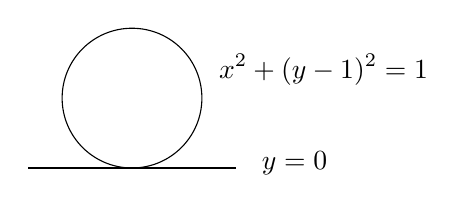
\begin{tikzpicture}[x=0.75pt,y=0.75pt,yscale=-1,xscale=1]
			%uncomment if require: \path (0,300); %set diagram left start at 0, and has height of 300
			
			%Straight Lines [id:da9022525264933119] 
			\draw    (44,106) -- (144,106) ;
			%Shape: Circle [id:dp5620106547865036] 
			\draw   (60.33,72.33) .. controls (60.33,53.74) and (75.41,38.67) .. (94,38.67) .. controls (112.59,38.67) and (127.67,53.74) .. (127.67,72.33) .. controls (127.67,90.93) and (112.59,106) .. (94,106) .. controls (75.41,106) and (60.33,90.93) .. (60.33,72.33) -- cycle ;
			
			% Text Node
			\draw (155.33,97) node [anchor=north west][inner sep=0.75pt]   [align=left] {$\displaystyle y=0$};
			% Text Node
			\draw (134.67,50) node [anchor=north west][inner sep=0.75pt]   [align=left] {$\displaystyle x^{2} +( y-1)^{2} =1$};
		\end{tikzpicture}
	\end{center}
	
	直观上, 直线与圆相切, 两者在相切处有一条公共的 ``无穷小线段''. 更一般地, 任意两条相切的曲线都有一条公共的形如 $D$ 的无穷小线段, 这便是两条曲线共同的切向量.
\end{example}

\paragraph{Kock--Lawvere 公理与导数}

~

\begin{axiom}
	{(Kock--Lawvere 公理)}
	对任意映射 $f \colon D \to R$, 存在唯一的 $a,b\in R$,
	使得
	$$
	f(d) = a + d\cdot b,\quad\forall d\in D.
	$$
	换言之, 作为 $R$-代数有
	$$
	\operatorname{Hom}(D,R) \simeq R[x]/(x^2).
	$$
\end{axiom}

Kock--Lawvere 公理反映了如下的直观: $R$ 上的一个函数在一个很小的邻域上近乎是一次函数.
由此, 我们立刻得到如下的推论.

\begin{propdef}
	{(导函数)}
	对任意函数 $f\colon R\to R$, 存在唯一的函数 $f' \colon R \to R$ 满足
	$$
	f(x+d) = f(x) + d \cdot f'(x),\quad \forall x\in R\,\forall d\in D.
	$$
	称 $f'$ 为 $f$ 的\emph{导函数}. 归纳地定义 $k$ 阶导数 $f^{(k)}(x)$.
\end{propdef}

任何函数都是任意次可导的.

\paragraph{Weil 代数与无穷小几何对象}

~

无穷小线段 $D$ 对应代数 $R[x]/(x^2)$. 一般地, 在代数--几何对偶中与无穷小几何对象相对应的代数是 \emph{Weil 代数}.
\begin{definition}
	{(Weil 代数)}
	Weil 代数是形如 $W = R \oplus J$ 的 $R$-代数,
	其中 $J$ 是有限生成自由 $R$-模,
	且为幂零理想.
\end{definition}

\begin{definition}
	{(Weil 代数的谱)}
	对于 Weil 代数 $W$, 定义 $W$ 的\emph{谱}为 $R$-代数同态的空间
	$$
	\operatorname{Spec}W = \operatorname{Hom}_{R\mathsf {Alg}}(W,R),
	$$
	称之为\emph{无穷小几何对象}.
\end{definition}

\begin{example}
	{(常见的无穷小几何对象)}
	\begin{itemize}
		\item 点 $$\text{pt} \simeq \{x\in R\mid x=0\} = \operatorname{Spec} R;$$
		\item 无穷小线段的平方 $$D^2 \simeq \{(x,y)\in R^2 \mid x^2=y^2=0\} = \operatorname{Spec}R[x,y]/(x^2,y^2);$$
		\item $R^2$ 上原点的一阶无穷小邻域 $$D(2) := \{(x,y)\in R^2\mid x^2=xy=y^2=0\} = \operatorname{Spec}R[x,y]/(x^2,xy,y^2);$$
		\item 高阶无穷小邻域
		$$
		D_k := \{x\in R\mid x^{k+1}=0\} = \operatorname{Spec}R[x]/(x^{k+1})\, (k=1,2,3,\cdots).
		$$
	\end{itemize}
\end{example}

前面介绍的 Kock--Lawvere 公理可表述为 $\operatorname{Hom}(\operatorname{Spec}R[x]/(x^2),R) \simeq R[x]/(x^2)$. 类似地有如下公理.

\begin{axiom}
	{(Kock--Lawvere 公理)}
	对于 Weil 代数 $W$, 有
	$$
	\operatorname{Hom}(\operatorname{Spec}W,R)\simeq W.
	$$
\end{axiom}

\begin{remark}
	{(Weil 代数与 Kock--Lawvere 公理的直观)}
	设 $W=R\oplus J$ 是 Weil 代数. 投影 $W \to R$ 对应点 $\text{pt}$ 到无穷小几何对象 $\operatorname{Spec}W$ 的\emph{原点}的嵌入 $$\text{pt} = \operatorname{Spec} R \to \operatorname{Spec}W.$$
	Kock--Lawvere 公理说的是 Weil 代数 $W$ 等同于 $\operatorname{Spec}W$ 上的函数代数. 投影 $W\to R$ 可视为 $\operatorname{Spec}W$ 上的函数在原点处取值; 理想 $J$ 是投影 $W\to R$ 的核, 可视为在原点取值为 $0$ 的函数的集合.
	要求 $J$ 为\emph{幂零}理想, 也即要求在原点取值为 $0$ 的函数都幂零, 直观上说明 $\operatorname{Spec}W$ 是 ``无穷小'' 的.
\end{remark}

\subsection{综合微分几何的模型}



\begin{definition}
	{}
	
\end{definition}

\section{量子理论与 Bohr 意象}



\subsection{$C^*$-代数, 经典语境与 Bohr 景}

一般而言, 量子系统是由 $C^*$-代数表示的.

\begin{remark}
    {(约定)}
    约定本章中的 ``代数'' 指含幺结合代数, 且代数的同态保持幺元.
\end{remark}

\begin{definition}
    {($C^*$-代数)}
    \emph{$C^*$-代数}是 $\mathbb{C}$ 上的 Banach 代数 $\big(\mathcal A,\|{-}\|\big)$,
    带有 ``伴随'' 运算 $(-)^*\colon \mathcal A \to \mathcal A$,
    满足对任意 $x\in \mathcal A$,
    \begin{itemize}
        \item $(x^*)^*=x$,
        \item $(xy)^*=y^*x^*$,
        \item $(\lambda x)^*=\bar\lambda x^*\,(\lambda\in\mathbb{C})$,
        \item $\|x^* x\|=\|x\|\|x^*\|=\|x\|^2$.
    \end{itemize}
    $C^*$-代数的 $*$-子代数是指关于 $(-)^*$ 封闭的子代数.
\end{definition}

\begin{example}
    {}
    对于 Hilbert 空间 $H$, $H$ 上的有界线性算子的代数 $\mathcal B(H)$ 是 $C^*$-代数, 其中 $x^*$ 是 $x$ 的伴随算子. 事实上, 每个 $C^*$-代数都同构于某个形如 $\mathcal B(H)$ 的代数的 $*$-子代数, 因此后者也可作为 $C^*$-代数的一种具体定义.
\end{example}

下面我们固定一个 $C^*$-代数 $\mathcal A$.

\begin{definition}
    {(可观测量)}
    $C^*$-代数中的自伴元素是指满足 $x^*=x$ 的元素; 自伴元素又称\emph{可观测量} (observable).
\end{definition}

Heisenberg 不确定性原理表明, 不交换的可观测量不可同时确定, 而一族相交换的可观测量可以同时确定. 因此我们格外关注那些交换的子代数.

\begin{definition}
    {(经典语境)}
    称 $\mathcal A$ 的一个交换 $*$-子代数为一个\emph{经典语境} (classical context).
    记 $\mathsf C(\mathcal A)$ 为 $\mathcal A$ 的交换 $*$-子代数在包含关系下构成的偏序集.
\end{definition}

\begin{remark}
    {}
    语境这个名字的含义是, 一个可观测量只在某些特定的语境 (也就是包含它的那些语境) 下才有确定的值. 在一个固定的语境中, 可观测量的表现无异于一个经典系统.
\end{remark}

这里我们稍微偏题, 介绍偏序集上的层.

\begin{definition}
    {(Alexandorff 空间)}
    若一个拓扑空间中开集的任意交仍是开集, 则称其为 \emph{Alexandorff 空间}.
\end{definition}

\begin{definition}
    {(Alexandroff 拓扑)}
    设 $P$ 为偏序集. 定义 $P$ 上的 \emph{Alexandroff 拓扑}是以向上封闭集为开集的拓扑. 其中, 称 $Q\subset P$ 为\emph{向上封闭集}是指对任意 $x\in Q,y\in P$, 若 $x\leq y$, 则 $y\in Q$.
\end{definition}

\begin{prop}
    {}
    对任意偏序集 $P$, $P$ 上的预层可自然延拓为 $P$ 的 Alexandroff 拓扑上的层.
\end{prop}

% sheaf vs cosheaf

\begin{definition}
    {(Bohr 景)}
    范畴, 也称 \emph{Bohr 景}. Bohr 景上的意象将是我们主要的研究对象.
\end{definition}

\section{Bohr 意象}

\begin{definition}
    {(Bohr 意象)}
    称 $\mathsf C(\mathcal A)$ 上的预层意象为 \emph{Bohr 意象}.
\end{definition}



\subsection{状态空间}

\begin{definition}
    {(Gelfand 谱)}
    对于交换 $C^*$-代数 $A$, 定义其 \emph{Gelfand 谱}
$$
\Sigma(A) := \{C^*\text{-代数同态}\,\lambda\colon A \to\mathbb{C}\},
$$
其拓扑为使得所有映射 $\Sigma(A)\to\mathbb{C}, \lambda \mapsto \lambda (x)$ 都连续的最弱拓扑. 由 Gelfand--Mazur 定理, Gelfand 谱 $\Sigma(A)$ 也是 $A$ 的极大理想的集合.
\end{definition}

$\Sigma(A)$ 上拓扑的定义旨在保证每个元素 $x\in A$ 都对应 $\Sigma(A)$ 上的一个复值连续函数. 如下定理表明这个对应实际上是一个同构; 这是代数--几何对偶的一例.

\begin{prop}
    {(Gelfand--Naimark 对偶)}
    记 $\mathsf {CC}^*$ 为交换 $C^*$-代数的范畴, $\mathsf{CHaus}$ 为紧 Hausdorff 空间的范畴,
    那么 Gelfand 谱给出反变函子 $\Sigma\colon \big(\mathsf {CC}^*\big)^{\op} \to \mathsf {CHaus}$, 且有范畴等价
    \[\begin{tikzcd}[ampersand replacement=\&]
    	{\big(\mathsf {CC}^*\big)^{\op}} \& {\mathsf {CHaus},}
    	\arrow["\Sigma", shift left, from=1-1, to=1-2]
    	\arrow["{C({-},\mathbb{C})}", shift left, from=1-2, to=1-1]
    \end{tikzcd}\]
    其中 $C(X,\mathbb{C})$ 是空间 $X$ 上复值连续函数的 $C^*$-代数.
\end{prop}

可观测量代数与状态空间互为对偶. 经典力学中, 可观测量是状态空间上的函数; 反过来, 状态空间上的点可视为可观测量代数到 $\mathbb{R}$ 的代数同态.
完全类似地, 在量子力学中, 给定语境 $A$, 对应的 "状态空间" $\Sigma(A)$ 中的点就是 $A$ 到 $\mathbb{C}$ 的代数同态, 而 $A$ 中的可观测量则可视为状态空间 $\Sigma(A)$ 上的函数.

\begin{definition}
    {(谱预层)}
    对于语境 $A_1 \subset A_2$, 有限制映射 $\Sigma(A_2)\to\Sigma(A_1)$. 这定义了 $\mathsf C(\mathcal A)$ 上的预层 $\Sigma$.
\end{definition}

\begin{remark}
    {}
    预层 $\Sigma$ 整合了所有经典语境的几何信息.
    
    一般而言, 一个可观测量只能给出预层 $\Sigma$ 的局部截面, 而无法给出整体截面.
\end{remark}

Bohr 意象中对象 $\Sigma$ 的构造可视为将 Gelfand 谱的构造由交换代数推广到非交换代数, 成为与交换子代数相对偶的空间的系统. 它实际上是 Bohr 意象中的内蕴位象 (internal locale). 而几乎是平凡地, 那些交换子代数的全体构成 Bohr 意象中的一个内蕴代数. 由此, Bohr 意象的内语言允许我们像谈论经典态一样谈论量子态.

\subsection{Bohr 意象中的命题}



在一个经典系统中, 命题是状态空间的子集, 表示这个命题在何种状态下成立.
类似地, 量子系统中的命题是预层意象中 $\Sigma$ 的子对象, 或称子函子.

\section{Cohen 力迫法}

\label{Cohen-forcing}

1874 年, Georg Cantor 证明了自然数与实数 (又称连续统) 之间不存在一一对应\footnote{不过他的第一个证明并非现在流行的对角线论证.}. Cantor 接着于 1878 年提出了\emph{连续统假设} (continuum hypothesis),
$$
\fbox{在自然数集合 $N$ 与连续统 $PN$ 之间不存在其它的基数.}
$$

1940 年, Kurt G\"odel 证明连续统假设与 Zermelo--Fraenkel 集合论相容. 1963 年, Paul Cohen 证明了连续统假设独立于带有选择公理的 Zermelo--Fraenkel 集合论 (ZFC), 即 ZFC 既不能证明, 也不能证伪连续统假设.

% Boole 意象的内容放在了第一章末尾.

在 \ref{Boolean-topos} 节我们介绍了 Boole \topos{}. 我们可以在这样的\topos{}中做 ``经典数学''. 下面的内容本质上等同于 Cohen 证明连续统假设独立于 ZFC 所使用的方法, 只不过翻译到了\topos{}的语境.

\begin{prop}
	{}
	存在一个 Boole \topos{}, 其中选择公理成立, 而连续统假设不成立.
\end{prop}

\subsubsection{基础知识}

回忆任何\topos{}上都有一个 Lawvere--Tierney 拓扑 $\neg\neg$. 有趣的是, 它总是给出一个 Boole 意象.

\begin{prop}
	{}
	对任意\topos{} $\mathcal C$, $\operatorname{Sh}_{\neg\neg}\mathcal C$ 为 Boole \topos{}.
\end{prop}
\begin{proof}
	由 Boole \topos{}的内语言刻画 (\ref{internal-Boolean-topos}), 我们要在 $\operatorname{Sh}_{\neg\neg}\mathcal C$ 中证明 $\forall p\in\Omega (p\lor \neg p)$.
	% 需要几何态射在命题上的作用
\end{proof}

\begin{definition}
	{(基数的比较)}
	对于一个\topos{}中的两个对象 $X,Y$, 若存在单射 $X\to Y$, 且 $\operatorname{Epi}(X,Y)\simeq 0$, 则称 $X$ 的基数小于 $Y$, 记为 $X<Y$.
\end{definition}

回忆 $\operatorname{Epi}(X,Y)$ 的定义 (\ref{set-of-epimorphisms}), $\operatorname{Epi}(X,Y)\simeq 0$ 当且仅当公式 $\forall f\in Y^X\,\neg(\operatorname{im}f = Y)$ 成立.



\section{凝聚态数学}

% 【潜水】岩豚鼠: 我们要解决拓扑abel群范畴不是abel范畴的问题, 首先要解决拓扑空间范畴中连续双射不可逆的问题. 注意到紧Hausdorff空间没有这个问题, 我们就尝试将一般的拓扑空间换成紧Hausdorff空间范畴上的层, 而这个景有一族基叫做投射有限集. 这里的拓扑是取连续满射为覆盖. 每个紧Hausdorff空间都被它自己的集合作为离散空间覆盖, 注意到紧Hausdorff空间到一般拓扑空间范畴的嵌入有个左伴随叫Stone—Cech紧化, 我们就可以把基取为离散空间的SC紧化.

作为原理的介绍, 本节忽视集合论问题.

\begin{definition}
	{(投射有限集景)}
	\emph{投射有限集景} $\mathsf{ProFin}$ 是投射有限集的范畴 (例 \ref{pro-finite-set}), 配备有限联合满射族生成的覆盖. 该覆盖对应 $\mathsf {ProFin}$ 上的典范 Grothendieck 拓扑 (定义 \ref{canonical-topology}).
\end{definition}

% 为什么典范?
% 紧空间上联合有效满射族必然有有限的子族构成联合满射.


\begin{definition}
	{(凝聚态集合)}
	\emph{凝聚态集合} (condensed set) 是投射有限集景 $\mathsf{ProFin}$ 上的层. 记凝聚态集合的范畴为 $\mathsf{Cond}$.
	定义凝聚态群 (Abel 群, 环, ...) 为 $\mathsf{Cond}$ 中的群 (Abel 群, 环, ...).
\end{definition}

任何一个 Grothendieck \topos{}中的 Abel 群构成 Abel 范畴. 凝聚态 Abel 群也构成一个 Abel 范畴. 相比之下, 拓扑 Abel 群范畴没有这样好的性质: 考虑 Abel 群 $\mathbb{R}$ 带有离散拓扑 $\mathbb{R}_{\text{散}}$ 和通常拓扑 $\mathbb{R}_{\text{常}}$. 恒等映射 $\mathbb{R}_{\text{散}}\to \mathbb{R}_{\text{常}}$ 既单又满, 却不是同构.

\begin{example}
	[label={top-space-as-cond-set}]
	{(拓扑空间视为凝聚态集合)}
	对于拓扑空间 $X$, 定义凝聚态集合 $\underline{X}\colon S\mapsto \operatorname{Hom}_{\mathsf {Top}}(S,X)$.
	当然, 对于拓扑群 (Abel 群, 环, ...), 也有相应的凝聚态群 (Abel 群, 环, ...).
	
	凝聚态集合 $\underline{X}$ 包含了 $X$ 的许多重要的拓扑信息. 例如, 考虑投射有限集 $\mathbb{N}\cup\infty$ (例 \ref{N-cup-infty}), $\underline{X}(\mathbb{N}\cup\infty)$ 的元素等同于 $X$ 中的\emph{收敛序列}.
	
	对于好的空间 $X$ (所谓\emph{紧生成 Hausdorff 空间}), $\underline{X}$ 包含的信息足够还原 $X$ 的拓扑, 这就是说这类拓扑空间的范畴全忠实地嵌入凝聚态集合范畴.
\end{example}

\begin{remark}
	[label={remark-topological-topos}]
	{(凝聚态集合作为拓扑空间的推广, Johnstone 拓扑\topos{})}
	由例 \ref{top-space-as-cond-set}, 凝聚态集合可视为拓扑空间的推广: 对于凝聚态集合 $X$ 与投射有限集 $S$, $X(S)$ 的元素可视为 $S$ 到 $X$ 的假想的 ``连续映射''; 
	特别地, $X(\mathbb{N}\cup\infty)$ 的元素可视为 $X$ 中假想的 ``收敛序列''.
	
	称拓扑空间 $X$ 为\emph{序列空间} (sequential space) 是指: 对任意拓扑空间 $Y$, 集合映射 $f\colon X\to Y$ 连续当且仅当 $f$ 将 $X$ 中的收敛序列映射到 $Y$ 中的收敛序列. 很多常见的拓扑空间 (如 CW 复形) 都是序列空间.
	考虑单点 $\text{pt}$ 和 $\mathbb{N}\cup\infty$ 构成的 $\mathsf {Top}$ 的全子范畴, 配备典范 Grothendieck 拓扑成为一个景, 这个景上的层范畴即是 Johnstone 的\emph{拓扑\topos{}} $\mathcal T$. 那么序列空间的范畴全忠实地嵌入 $\mathcal T$, 正如紧生成 Hausdorff 空间全忠实地嵌入凝聚态集合范畴一样.
\end{remark}


% 第五章 分类\topos{}
\chapter{句法景与分类\topos{}}

\label{cla}

\minitoc

\section{句法范畴: 语法--语义对偶}

% \todo{两种不同的 syntactic category}

%\todo{写成单独的一章?}

\philoquote{The importance of syntactic categories lies in the fact that they allow us to associate with a theory (in the sense of axiomatic presentation), which is a `linguistic',
	unstructured kind of entity, a well-structured mathematical object whose `geometry' embodies the syntactic aspects of the theory.}{Olivia Caramello, \cite{TST}}

%  A most notable fact is that the models of the theory can be recovered as functors defined on its syntactic category which respect the ‘logical’ structure on it.

范畴逻辑学的一个一般性的现象是理论 (一阶逻辑, 类型论等等) 与范畴之间的对应. 某些范畴可以为理论提供语义, 某些理论可以作为范畴的语法.
语法--语义对偶也是一种代数--几何对偶\footnote{或许也可以反过来说代数--几何对偶不过是一种语法--语义对偶.}, 语法是 ``代数'', 语义是 ``几何''.
这一点已经在 \ref{locales-and-logic} 节体现.

\subsection{代数理论的句法范畴}

% 建议不熟悉 Lawvere 理论的读者先阅读附录 \ref{universal-algebra} 节.

\begin{prop}
	{}
	对于 Horn 理论 $\mathbb T$,
\end{prop}





\subsection{一阶理论的句法范畴}

\begin{definition}
	[label={first-order-theory-syntactic-category}]
	{(一阶理论的句法范畴)}
	
	设 $\mathbb T$ 是符号表 $\Sigma$ 上的一阶理论. 定义\emph{句法范畴} (syntactic category) $\mathcal C_{\mathbb T}$ 为如下的范畴,
	\begin{itemize}
		\item 其对象是 $\Sigma$ 上带语境的公式 $(\vec x , \phi)$ 的 $\alpha$-等价类, $\alpha$ 等价是指两个公式仅有变量名的差异. 公式的种类由理论 $\mathbb T$ 的类别规定, 如几何理论允许使用几何公式, 正则理论允许使用正则公式, 代数理论只允许使用形如\todo{TST p46}
		\item 对象 $(\vec x , \phi)$ 到 $(\vec y , \psi)$ 的态射 (其中不妨设语境 $\vec x , \vec y$ 不交) 是公式 $\theta(\vec x,\vec y)$ 的 $\mathbb T$-可证等价类, 满足 $\mathbb T$-可证的\emph{函数性}, 即如下相继式 $\mathbb T$-可证.
		\begin{itemize}
			\item $\phi\vdash_{\vec x} \exists \vec y \,\theta$, 含义是 ``对给定的 $\vec x$, 存在 $\vec y$ 满足 $\theta(\vec x,\vec y)$'';
			\item $\theta\vdash_{\vec x,\vec y} \phi \wedge \psi$,
			\item $\theta \wedge \theta[\vec z/\vec y] \vdash_{\vec x,\vec y,\vec z} \vec y = \vec z$, 这里 $\theta[\vec z / \vec y]$ 是指将 $\theta$ 中的 $\vec y$ 替换为 $\vec z$, 公式的含义是 ``对给定的 $\vec x$, 至多存在一个 $\vec y$ 满足 $\theta(\vec x,\vec y)$''.
		\end{itemize}
	\end{itemize}
\end{definition}

\begin{remark}
	{}
	句法范畴的态射又称\emph{变量代换}.
\end{remark}

\begin{remark}
	{}
	由定义, 一个理论的句法范畴依赖于理论所属的类别 (代数, 正则, 凝聚, $\cdots$). 一个代数理论也可以视为凝聚理论, 但一个代数理论的句法范畴与它作为凝聚理论的句法范畴不同.
\end{remark}

\begin{example}
	{(环的句法范畴)}
	%对于通常背景的读者, 或许最合适的例子是环的理论的句法范畴.
	回忆, 环的理论是一种代数理论, 其中的公式形如 $s=t$.
\end{example}

\subsection{类型论的语境范畴}

附录 \ref{appendix-type-theory} 节简单介绍了类型论.

\begin{definition}
	{}
	对于一种类型论 $T$, 其\emph{语境范畴} (category of contexts) $\operatorname{Con}(T)$ 定义如下.
	\begin{itemize}
		\item $\operatorname{Con}(T)$ 的\emph{对象}为类型论 $T$ 的\emph{语境};
		\item $\operatorname{Con}(T)$ 中的\emph{态射}为语境之间的\emph{代换}.
	\end{itemize}
\end{definition}

\section{分类\topos{}}

\philoquote{
    The notion of classifying topos really formalizes the notion of ``content'' of a mathematical theory.
    If you discover that two theories have the same classifying topos, this means that the two theories tell the same story in different languages.
}{Olivia Caramello}

% https://q.uiver.app/#q=WzAsNCxbMSwxLCJcXHRleHR75YiG57G7XFx0b3Bvc3t9fSJdLFsxLDAsIlxcdGV4dHvliIbnsbvnqbrpl7R9Il0sWzAsMCwiXFx0ZXh0e+epuumXtH0iXSxbMCwxLCJcXHRleHR7XFx0b3Bvc3t9fSJdLFsyLDMsIiIsMCx7InN0eWxlIjp7ImJvZHkiOnsibmFtZSI6InNxdWlnZ2x5In19fV0sWzEsMCwiIiwwLHsic3R5bGUiOnsiYm9keSI6eyJuYW1lIjoic3F1aWdnbHkifX19XV0=
\[\begin{tikzcd}[ampersand replacement=\&]
	{\text{空间}} \& {\text{分类空间}} \\
	{\text{\topos{}}} \& {\text{分类\topos{}}}
	\arrow[squiggly, from=1-1, to=2-1]
	\arrow[squiggly, from=1-2, to=2-2]
\end{tikzcd}\]

~\\

%分类\topos{}的角色类似于拓扑学中的分类空间:
在代数拓扑中, 对于拓扑群 $G$ 可构造\emph{分类空间} $BG$,
使得 (足够好的) 空间 $X$ 上 $G$-主丛的等价类
一一对应于 $X$ 到 $BG$ 的映射同伦类 (被 $BG$ ``分类''),
$$
G\mathsf{Bund} (X) \simeq [X,BG];
$$
从而恒等映射 $\operatorname{id}_{BG}$ 对应着 $BG$ 上一个\emph{万有 $G$-主丛} $EG \to BG$,
``万有'' 意指任何 $G$-主丛都是通过某个映射 $X \to BG$ 将其拉回得到.

类似地, 在许多情形下, \topos{} $\mathcal C$ 上的一种结构 $T$ (即某个理论的模型) 可由它到一个特殊的\topos{}的态射来分类, 这就是\emph{分类\topos{}}的概念;
某种结构 $T$ 的分类\topos{}可视为 ``所有 $T$ 构成的空间'', 也可称作 $T$ 的\emph{模空间}.
若将\topos{} $\mathcal C$ 视为空间, 那么 $\mathcal C$ 上的一个结构 $T$ 可视为空间的 ``每一点'' 上都有一个结构 $T$,
从而这给出 $\mathcal C$ 到模空间的一个几何态射.
例如, 设 $\mathcal E$ 为环的分类\topos{}, 那么 $\mathcal E$ 应当视为 ``所有环构成的空间'' (上的层范畴), 拓扑空间 $X$ 上的一个环层即是 $X$ 的 ``每一点'' 上都有一个环,
这等同于 $\text{Sh}(X)$ 到 $\mathcal E$ 的一个几何态射.
与分类空间的情况类似, 分类\topos{}到自身的恒等态射对应着其上的 ``\emph{万有 $T$ 结构}'', 又称\emph{重言} (tautological) $T$ 结构.

\subsection{例}

\subsubsection{$G$-旋子的分类\topos{}}

\begin{definition}
	{(群作用)}
	设 $\mathcal C$ 为\topos{}, $G$ 为 $\mathcal C$ 中的群, 其乘法映射与单位元分别为 $m\colon G\times G\to G$, $e\colon 1\to G$. 设 $X$ 为 $\mathcal C$ 的对象. 定义 $X$ 上的 $G$-\emph{左作用}为一个映射 $\rho\colon G\times X\to X$, 满足如下交换图.
	% https://q.uiver.app/#q=WzAsNyxbMSwwLCJHXFx0aW1lcyBYIl0sWzAsMCwiR1xcdGltZXMgR1xcdGltZXMgWCJdLFswLDEsIkdcXHRpbWVzIFgiXSxbMSwxLCJYIl0sWzIsMCwiWCJdLFszLDEsIlgiXSxbMywwLCJHXFx0aW1lcyBYIl0sWzEsMiwibSIsMl0sWzEsMCwiXFxyaG8iXSxbMiwzLCJcXHJobyIsMl0sWzAsMywiXFxyaG8iXSxbNCw1LCJcXG9wZXJhdG9ybmFtZXtpZH1fWCIsMl0sWzQsNiwiZSJdLFs2LDUsIlxccmhvIl1d
	\[\begin{tikzcd}[ampersand replacement=\&]
		{G\times G\times X} \& {G\times X} \& X \& {G\times X} \\
		{G\times X} \& X \&\& X
		\arrow["m"', from=1-1, to=2-1]
		\arrow["\rho", from=1-1, to=1-2]
		\arrow["\rho"', from=2-1, to=2-2]
		\arrow["\rho", from=1-2, to=2-2]
		\arrow["{\operatorname{id}_X}"', from=1-3, to=2-4]
		\arrow["e", from=1-3, to=1-4]
		\arrow["\rho", from=1-4, to=2-4]
	\end{tikzcd}\]
	等价地, 群作用也可定义为半群的同态 $G\to X^X$.
\end{definition}

%\begin{definition}
%	{(普通的群视为\topos{}中的群)}
%	设 $G$ 为 ($\mathsf {Set}$ 中的) 群, $\gamma\colon \mathcal C\to \mathsf {Set}$ 是 $\mathsf {Set}$ 上的\topos{} (见命题 \ref{global-sections-geometric-morphism}). 那么 $\gamma^*(G)$ 为 $\mathcal C$ 中的群. 为了记号的简便, 我们以 $G$ 表示 $\gamma^*(G)$.
%	%因为 $\gamma^*$ 保持有限极限 (特别地, $\gamma^*(1)=1$), 所以 $\gamma^*(G)$ 是群.
%	对于群 $G$ 的元素 $g\colon 1\to G$, 以 $g$ 表示其给出的 $\gamma^*(G)$ 的整体元素 $\gamma^*(g)\colon 1\to \gamma^*(G)$.
%\end{definition}

下面的概念是 ``空间上的 $G$-主丛'' 的推广, 取自 \cite{SGL} VIII.2 节.
\begin{definition}
	[label={G-torsors-over-topos}]
	{(\topos{}上的 $G$-旋子)}
	设 $G$ 为群. 定义 $\mathcal C$ 上的一个 $G$-\emph{旋子}\footnotemark (torsor) 为 $\mathcal C$ 的对象 $T$, 以及 $\underline G$ (记号见注 \ref{notation-constant-sheaf}) 在 $T$ 上的作用 $\mu\colon \underline G\times T \to T$, 满足
	\begin{enumerate}[(i)]
		\item 映射 $T\to 1$ 为满射, 即 $T$ ``有物'' (关于有物与非空的讨论, 见 \ref{inhabited-vs-nonempty});
		\item 群作用 $\mu$ 诱导同构 $(\mu,\pi_2)\colon \underline G\times T \to T\times T$.
	\end{enumerate}
	记 $\mathcal C$ 上的 $G$-旋子构成范畴为 $\mathsf{Tors}_G(\mathcal C)$, 其中态射是保持 $G$-左作用的映射.
\end{definition}
\footnotetext{Torsor 似乎没有通行的中文译名, 这可能是因为它在拓扑学中一般被称作\emph{主丛}. 这里我跟随我的一位老师将其译为\emph{旋子}.}

%\begin{remark}
%	{(条件 ii 的解读)}
%	群作用 $\mu$ 诱导同构 $(\mu,\pi_2)\colon \gamma^*(G)\times T \to T\times T$ 等价于 $\gamma^*(G)$ 在 $T$ 上的作用是自由且传递的.
%	
%\end{remark}

\begin{example}
	{(集合范畴中的 $G$-旋子)}
	由于集合范畴 $\mathsf {Set}$ 是一个点上的层范畴,
	$\mathsf {Set}$ 中的 $G$-旋子即是 ``一个点上的 $G$-主丛'',
	即一个非空集合 $T$, 带有 $G$-左作用 $\mu\colon G\times T \to T$, 满足 $(\mu,\pi_2)\colon G\times T \to T\times T$ 为双射.
	后一个条件等价于这个作用是自由且传递的:
	``自由'' 等价于 $(\mu,\pi_2)\colon G\times T \to T\times T$ 为单射, ``传递'' 等价于其为满射.
	
	另一种看法是, 两个映射 $\mu,\pi_2\colon G\times T \to T$ 给出了一个范畴 (具体地, $G$ 在 $T$ 上作用的\emph{作用群胚}) 的箭头集合到对象集合的两个映射, 分别将一个箭头映射到其终点与起点. 那么 $(\mu,\pi_2)\colon G\times T \to T\times T$ 为双射就是说, 作用群胚的任何两个对象 $x,y$ 之间有且仅有一个态射 $x\to y$.
\end{example}

\begin{example}
	{(空间上的 $G$-主丛)}
	仍设 $G$ 为离散群. 拓扑空间 $X$ 上的 $G$-主丛等价于平展映射 $E \to X$, 带有 $X$ 上的 $G$-左作用 $\underline G\times E \to E$, 使得每个纤维 $E_x$ 非空且带有 $G$ 的自由传递作用. 这等价于层\topos{} $\operatorname{Sh}(X)$ 上的 $G$-旋子.
\end{example}

就像分类空间 $BG$ 上有万有 $G$-主丛, \topos{} $G\mathsf {Set}$ 上有\emph{万有 $G$-旋子}; 它就是 $G$ 在自身上的 $G$-右作用, 记为 $R_G$.

首先说明 $R_G$ 是 $G\mathsf {Set}$ 上的 $G$-旋子.
回忆几何态射 $\gamma\colon G\mathsf {Set} \to \mathsf {Set}$ (例 \ref{group-homomorphism-adjoint-triple-example-G-1}), 其逆像函子 $\gamma^*\colon \mathsf {Set} \to G\mathsf {Set}$ 将集合对应到其自身, 带有平凡 $G$-右作用; 直像函子 $\gamma_*\colon G\mathsf {Set}\to\mathsf {Set}$ 将 $G$-集合对应到其不动点集.
群作用 $\mu\colon \underline G\times R_G \to R_G$, $(g,h)\mapsto gh$ 是 $G$-集合的态射, 因为\emph{左作用与右作用交换},  $\mu(g,hk)=ghk=\mu(g,h)k$.
映射 $(\mu,\pi_2)\colon \underline G\times R_G\to R_G\times R_G$ 为 $(g,h)\mapsto (gh,h)$, 从而为 $G$-集合的同构.

\begin{prop}
	{(万有 $G$-旋子)}
	$R_G$ 是万有 $G$-旋子, 即对任何\topos{} $\mathcal C$ 上的 $G$-旋子 $T$, 有一对伴随
	% https://q.uiver.app/#q=WzAsMixbMCwwLCJcXG1hdGhjYWwgQyJdLFsxLDAsIkdcXG1hdGhzZiB7U2V0fSJdLFswLDEsIlxcb3BlcmF0b3JuYW1le0hvbX1fe1xcbWF0aGNhbCBDfShULC0pIiwyLHsib2Zmc2V0IjoyfV0sWzEsMCwiVFxcdGltZXNfe0d9IC0iLDIseyJvZmZzZXQiOjJ9XSxbMywyLCIiLDAseyJsZXZlbCI6MSwic3R5bGUiOnsibmFtZSI6ImFkanVuY3Rpb24ifX1dXQ==
	\[\begin{tikzcd}[ampersand replacement=\&]
		{\mathcal C} \& {G\mathsf {Set},}
		\arrow[""{name=0, anchor=center, inner sep=0}, "{\operatorname{Hom}_{\mathcal C}(T,-)}"', shift right=2, from=1-1, to=1-2]
		\arrow[""{name=1, anchor=center, inner sep=0}, "{-\times_{G}T}"', shift right=2, from=1-2, to=1-1]
		\arrow["\dashv"{anchor=center, rotate=-90}, draw=none, from=1, to=0]
	\end{tikzcd}\]
	且有 $T\simeq R_G\times_G T$. 这一构造给出了范畴等价
	\[
	\mathsf{Tors}_G(\mathcal C)\simeq\operatorname{Hom}_{\Top}(\mathcal C,G\mathsf {Set}).
	\]
\end{prop}
顾名思义, 这对伴随是 ``张量--同态伴随'' 的类比, 参见命题 \ref{group-action-tensor-hom}, \ref{presheaf-topos-tensor-hom-adjunction}.
\begin{proof} 略. 我们仅给出这一对函子的定义.
\begin{itemize}
	\item 因为 $T$ 带有 $G$-左作用, 所以对 $\mathcal C$ 的对象 $X$, $\operatorname{Hom}_{\mathcal C}(T,X)$ 带有自然的 $G$-右作用. 这给出了函子 $\operatorname{Hom}_{\mathcal C}(T,-)\colon \mathcal C\to G\mathsf {Set}$.
	\item 设集合 $Y$ 带有 $G$-右作用. 定义 $\mathcal C$ 的对象 $Y\times_G T$ 为
	\[
	Y\times_G T := \operatorname{coeq}\big(
		\begin{tikzcd}[ampersand replacement=\&]
			{\underline Y\times \underline G \times T} \& {\underline Y\times T}
			\arrow[shift left, from=1-1, to=1-2]
			\arrow[shift right, from=1-1, to=1-2]
		\end{tikzcd}
	\big),
	\]
	其中两个映射分别是 $\underline G$ 右作用于 $\underline Y$ 和左作用于 $T$. 参考定义 \ref{group-action-tensor}.
\end{itemize}
\end{proof}



\topos{}上的旋子是一个理论的模型.

\begin{definition}
	{($G$-旋子的理论)}
	设 $G$ 为离散群, 定义 $G$-旋子的理论 $\mathbb T_G$.
	其中只有一个类型 $T$, 对每个元素 $g\in G$ 都有一个一元函数符号 $g$, 公理如下.
	\begin{itemize}
		\item (\emph{群作用}) 对每一对 $g,h\in G$ 有一条公理 $\vdash_x g(hx)=(gh)x$ (注意这里没有用到任意量词 $\forall$);
		\item (\emph{有物}) $\vdash \exists x. \top$;
		\item (\emph{自由性}) 对每一对不同的 $g,h\in G$ 有一条公理 $(gx=hx)\vdash_x \bot$ (同上, 这里没有用到 $\forall$);
		\item (\emph{传递性}) $\displaystyle\vdash_{(x,y)}\bigvee_{g\in G}gx=y$.
	\end{itemize}
\end{definition}

理论 $\mathbb T_G$ 是一种几何理论 (定义 \ref{kinds-of-theories}), 因为它用到了 ``真'' $\top$, 存在量词 $\exists$, ``假'' $\bot$ 和无穷析取 $\bigvee$.

\subsubsection{子终对象的分类\topos}

考虑范畴 $\mathsf 2 = \{\bullet\longrightarrow\bullet\}$. 例 \ref{varying-set-topos} 介绍的 ``变集范畴'' $\mathsf {Fun}(\mathsf {2},\mathsf {Set})\simeq\widehat {\mathsf {2}}$ 还有一个特殊的名字叫 \emph{Sierpi\'nski \topos{}}, 因为它与 Sierpi\'nski 空间有关.

\begin{propdef}
	[label={Sierpinski-space}]
	{(Sierpi\'nski 空间)}
	开集函子 $\operatorname{Open}\colon \mathsf {Top}\to \mathsf {Set}$ 是可表函子, 其表示对象称为 \emph{Sierpi\'nski 空间}.
\end{propdef}

\todo{}

\subsubsection{群的分类\topos{}}

本节构造群的分类\topos{}. 群是一种 Lawvere 理论 (附录 \ref{universal-algebra} 节); 下面的论述适用于一般的 Lawvere 理论, 从而逐字逐句地替换可得到环, Boole 代数等结构的分类\topos{}.
%
% 回忆范畴中的群对象的概念. 设范畴 $\mathcal C$ 有有限积 (包括始对象 $1$), 那么 $\mathcal C$ 中的\emph{群}为对象 $G$, 带有元素 $e \colon 1 \to G$, 乘法 $\cdot \colon G\times G \to G$, 满足群的交换图.

%满足通常的交换环的图表, 例如分配律 $x(y+z)=xy+xz$ 对应交换图
%% https://q.uiver.app/#q=WzAsNCxbMCwwLCJSXFx0aW1lcyBSXFx0aW1lcyBSIl0sWzEsMCwiUlxcdGltZXMgUiJdLFsxLDEsIlIiXSxbMCwxLCJSXFx0aW1lcyBSIl0sWzAsMSwiKHgseSx6KVxcbWFwc3RvICh4LHkreikiXSxbMSwyLCJcXHRpbWVzIl0sWzAsMywiKHgseSx6KVxcbWFwc3RvICh4eSx4eikiLDJdLFszLDIsIisiLDJdXQ==
%\[\begin{tikzcd}[ampersand replacement=\&]
%	{R\times R\times R} \& {R\times R} \\
%	{R\times R} \& R.
%	\arrow["{(x,y+z)}", from=1-1, to=1-2]
%	\arrow["\times", from=1-2, to=2-2]
%	\arrow["{(xy,xz)}"', from=1-1, to=2-1]
%	\arrow["{+}"', from=2-1, to=2-2]
%\end{tikzcd}\]
%(这里使用了 \ref{Mitchell--Benabou-language} 节介绍的 Mitchell--B\'enabou 语言.)

设范畴 $\mathcal C$ 有有限积. $\mathcal C$ 中的群对象构成一个范畴 $\mathsf {Grp}(\mathcal C)$.
\ref{universal-algebra} 节提到它等同于群的 Lawvere 理论 $\mathbb T_{\text{Grp}}$ 到 $\mathcal C$ 的保持有限积的函子的范畴.
进一步, 对于两个具有有限积的范畴 $\mathcal C,\mathcal D$, 以及保持有限积的函子 $f \colon \mathcal C \to \mathcal D$, 有对应的函子
$\mathsf {Grp}(\mathcal C) \to \mathsf {Grp}(\mathcal D)$.% $\mathsf {Ring}(\mathcal C) \to \mathsf {Ring}(\mathcal D)$.

对于\topos{}间的几何态射 $f \colon \mathcal C \to \mathcal D$, 其逆像部分 (见定义 \ref{geometric-morphism}) $f^* \colon \mathcal D \to \mathcal C$ 保持有限极限, 故保持有限积, 从而诱导了函子 $\mathsf {Grp}(\mathcal D) \to \mathsf {Grp}(\mathcal C)$;
这表示 $\mathsf {Grp}(-)$ 关于\topos{}是 ``反变'' 的.

下面我们将构造一个\topos{} $\mathcal E$, 称为\emph{群的分类\topos{}}, 使得有自然的范畴等价
$$
\mathsf {Grp}(\mathcal C) \simeq \mathsf{Hom}(\mathcal C,\mathcal E).
$$

\subsubsection{环的分类\topos{}}

\todo{单独讲一下和代数几何的关系}

% 参考 Caramello 的 TST

%\paragraph{群}
%
%考虑范畴 $\mathsf A = (\mathsf {Grp}_{\text{f}})^\op$,
%
%\paragraph{环}
%
%考虑范畴 $\mathsf A = (\mathsf {Ring}_{\text{fp}})^\op$,
%其中 $\mathsf {Ring}_{\text{fp}}$ 是 ($\mathsf{Set}$ 中) \emph{有限表现} (finitely presented) 环的范畴 (见例 \ref{zariski-site}).
%$\mathsf A$ 中有一个特殊的对象 $A = \mathbb{Z}[x]$,
%也即仿射直线.

\subsection{几何理论的分类\topos{}}

\todo{几何命题理论的 ``分类位象''}
\ref{classifying-locale}

\begin{definition}
    {(几何理论的句法景和分类\topos{})}
    设 $\mathbb T$ 为一几何理论.
    
    $\text{Sh}(\mathcal C_{\mathbb T},)$
\end{definition}

\todo{以 torsor 的句法景举例}

% 第六章 高阶范畴与高阶\topos{}
\chapter{高阶\topos{}}

\section{$\infty$-范畴}

粗略地说, 一个 $\infty$-范畴含有如下成分: 对象, 对象之间的态射, 态射之间的 $2$-态射, $\cdots$, $k$-态射之间的 $(k+1)$-态射, 以至于无穷. 在实践中, $\infty$-范畴有许多不同而互相等价的模型, 就像一个算法由许多不同的编程语言实现. 单纯集 (定义 \ref{Simplicial-Sets}) 就是一种实用的 ``编程语言''. 如下是用单纯集表达的一种 $\infty$-范畴的模型, 是 Lurie \cite{HTT} 使用的模型, 也是最简单的模型.

\begin{definition}
	{}
	定义单纯集 $\Delta^n$ 为米田嵌入的像 $\yo([n])$. 对于单射 $[m]\to [n]$, 设其像为 $J$, 定义单纯集 $\Delta^J$ 为对于 $0\leq k \leq n$, 定义 $\Lambda_k^n$ 为 $\Delta^n$ 包含顶点 $k$ 的各面之并, 称为\emph{角形} (horn).
\end{definition}

\begin{definition}
	{($\infty$-范畴)}
	\emph{$\infty$-范畴}是满足如下条件的单纯集 $X$: 对所有整数 $0<k<n$,
	$$
	\operatorname{Hom}(\Delta^n,X) \to \operatorname{Hom}(\Lambda_k^n,X)
	$$
	是满射. $\infty$-范畴之间的态射是单纯集的态射.
\end{definition}

\begin{definition}
	{($\infty$-群胚)}
\end{definition}

正如集合范畴 $\mathsf {Set}$ 是范畴的 ``原型'', 在 $\infty$-范畴中, 扮演这个角色的是某种 ``空间的范畴'', 其中各阶态射表达了空间之间映射的同伦.


\appendix

% 附录 范畴论
\chapter{范畴论基础}

\section{伴随函子}

\subsection{伴随保持极限}

\begin{prop}
	[label={adjoints-preserve-limits}]
	{}
	右伴随保持极限, 左伴随保持余极限.
\end{prop}

\begin{proof}
	设有伴随
	% https://q.uiver.app/#q=WzAsMixbMCwwLCJcXG1hdGhzZiB7Q30iXSxbMSwwLCJcXG1hdGhzZiB7RH0iXSxbMSwwLCJGIiwyLHsib2Zmc2V0IjoyfV0sWzAsMSwiRyIsMix7Im9mZnNldCI6Mn1dLFsyLDMsIiIsMCx7ImxldmVsIjoxLCJzdHlsZSI6eyJuYW1lIjoiYWRqdW5jdGlvbiJ9fV1d
	\[\begin{tikzcd}[ampersand replacement=\&]
		{\mathsf {C}} \& {\mathsf {D},}
		\arrow[""{name=0, anchor=center, inner sep=0}, "F"', shift right=2, from=1-2, to=1-1]
		\arrow[""{name=1, anchor=center, inner sep=0}, "G"', shift right=2, from=1-1, to=1-2]
		\arrow["\dashv"{anchor=center, rotate=-90}, draw=none, from=0, to=1]
	\end{tikzcd}\]
	设 $X \colon I \to \mathsf C$ 是一个图 ($I$ 是小范畴).
	若极限 $\lim_i X_i$ 存在,
	则有自然同构
	\begin{align*}
		\operatorname{Hom}(-,G\lim_i X_i)
		&\simeq \operatorname{Hom}(F-,\lim_i X_i)\\
		&\simeq \lim_i \operatorname{Hom}(F-,X_i)\\
		&\simeq \lim_i \operatorname{Hom}(-,GX_i)\\
		&\simeq \operatorname{Hom}(-,\lim_i GX_i).
	\end{align*}
	由米田引理, 得同构 $G\lim_i X_i \simeq \lim_i GX_i$,
	故右伴随保持极限.
	另一结论由对偶性即证.
\end{proof}

\begin{example}
	{}
	遗忘函子 $\mathsf {Top} \to \mathsf {Set}$ 同时有左伴随和右伴随:
	% https://q.uiver.app/#q=WzAsMixbMCwwLCJcXG1hdGhzZiB7VG9wfSJdLFsyLDAsIlxcbWF0aHNmIHtTZXR9Il0sWzAsMSwiXFx0ZXh0e+mBl+W/mH0iLDAseyJsYWJlbF9wb3NpdGlvbiI6MjB9XSxbMSwwLCLnprvmlaMiLDIseyJsYWJlbF9wb3NpdGlvbiI6MjAsIm9mZnNldCI6NX1dLFsxLDAsIuW5s+WHoSIsMCx7ImxhYmVsX3Bvc2l0aW9uIjoyMCwib2Zmc2V0IjotNX1dLFszLDIsIiIsMSx7ImxldmVsIjoxLCJzdHlsZSI6eyJuYW1lIjoiYWRqdW5jdGlvbiJ9fV0sWzIsNCwiIiwxLHsibGV2ZWwiOjEsInN0eWxlIjp7Im5hbWUiOiJhZGp1bmN0aW9uIn19XV0=
	\[\begin{tikzcd}[ampersand replacement=\&]
		{\mathsf {Top}} \&\& {\mathsf {Set}}
		\arrow[""{name=0, anchor=center, inner sep=0}, "{\text{遗忘}}"{pos=0.2}, from=1-1, to=1-3]
		\arrow[""{name=1, anchor=center, inner sep=0}, "{\text{离散}}"'{pos=0.2}, shift right=5, from=1-3, to=1-1]
		\arrow[""{name=2, anchor=center, inner sep=0}, "{\text{平凡}}"{pos=0.2}, shift left=5, from=1-3, to=1-1]
		\arrow["\dashv"{anchor=center, rotate=-90}, draw=none, from=1, to=0]
		\arrow["\dashv"{anchor=center, rotate=-90}, draw=none, from=0, to=2]
	\end{tikzcd}\]
	因此这个遗忘同时保持极限与余极限; 换言之, 拓扑空间的极限与余极限可用底层集合的极限与余极限来计算.
\end{example}

\begin{prop}
	[label={adjoint-full-subcategory-equivalence}]
	{(伴随产生一对满子范畴的等价)}
	设有伴随
	% https://q.uiver.app/#q=WzAsMixbMCwwLCJcXG1hdGhzZiB7Q30iXSxbMSwwLCJcXG1hdGhzZiB7RH0iXSxbMSwwLCJGIiwyLHsib2Zmc2V0IjoyfV0sWzAsMSwiRyIsMix7Im9mZnNldCI6Mn1dLFsyLDMsIiIsMCx7ImxldmVsIjoxLCJzdHlsZSI6eyJuYW1lIjoiYWRqdW5jdGlvbiJ9fV1d
	\[\begin{tikzcd}[ampersand replacement=\&]
		{\mathsf {C}} \& {\mathsf {D},}
		\arrow[""{name=0, anchor=center, inner sep=0}, "F"', shift right=2, from=1-2, to=1-1]
		\arrow[""{name=1, anchor=center, inner sep=0}, "G"', shift right=2, from=1-1, to=1-2]
		\arrow["\dashv"{anchor=center, rotate=-90}, draw=none, from=0, to=1]
	\end{tikzcd}\]
	其单位和余单位分别为
	$\eta \colon \operatorname{id}_{\mathsf D} \to GF$,
	$\epsilon \colon FG \to \operatorname{id}_{\mathsf C}$.
	考虑
	\begin{itemize}
		\item $\mathsf C$ 中由使得 $\eta_X \colon X \to GF(X)$ 为同构的 $X$ 构成的满子范畴 $\widetilde {\mathsf C}$,
		以及
		\item $\mathsf D$ 中由使得 $\epsilon_Y \colon FG(Y)\to Y$ 为同构的 $Y$ 构成的满子范畴 $\widetilde {\mathsf D}$,
	\end{itemize}
	那么 $F$ 与 $G$ 限制为一对互逆的范畴等价
	$$
	\widetilde G\colon \widetilde {\mathsf C} \overset{\simeq}{\to} \widetilde {\mathsf D},\quad
	\widetilde F\colon \widetilde {\mathsf D} \overset{\simeq}{\to} \widetilde {\mathsf C}.
	$$
\end{prop}

\begin{proof}
	由条件, $\eta$ 限制为自然变换
	$$
	\widetilde \eta \colon
	\operatorname{id}_{\widetilde {\mathsf D}} \to \widetilde G \widetilde F,
	$$
	且 $\widetilde \eta$ 的每个分量 ${\widetilde \eta}_{X} \colon X \to \widetilde G \widetilde F (X)$ 均为同构.
	因此 $\widetilde \eta$ 为自然同构. 另一边类似.
\end{proof}
\section{预层范畴与米田引理}

固定如下记号: $\mathsf C$ 为小范畴, $\yo\colon \mathsf C \to \widehat {\mathsf C} = \mathsf {Fun}(\mathsf C^{\op},\mathsf {Set})$ 为米田嵌入. 本节参考了 \cite{SGL} I.5 节.

\label{yoneda}

\subsection{可表函子的余极限}

\begin{definition}
    [label={slice-over-presheaf}]
    {(元素的范畴)}
    对 $X\in\widehat {\mathsf C}$, 定义 $X$ 的\emph{元素的范畴} $\displaystyle\int_{\mathsf C}X$ 如下.
    其对象为 $(c,x)$, $x\in X(c)$,
    态射 $(c,x)\to (d,y)$ 为 $f\colon c\to d$, 满足 $f(x)=y$.
    
    %记 $X$ 的元素的范畴为
    由定义, 存在 ``投影'' 函子 $\pi_X\colon \displaystyle\int_{\mathsf C}X\to \mathsf C$, $(c,x)\mapsto c$.
\end{definition}



\begin{remark}
    {(元素的范畴同构于 ``广义俯范畴'')}
    由米田引理, $X$ 的元素的范畴同构于如下范畴: 其对象为态射 $\yo(c)\to X$, 其态射为形如
    $\begin{tikzcd}[ampersand replacement=\&,row sep=-1pt,column sep=small]
    	{\yo(c)} \\
    	\& X \\
    	{\yo(d)}
    	\arrow[from=1-1, to=2-2]
    	\arrow[from=1-1, to=3-1]
    	\arrow[from=3-1, to=2-2]
    \end{tikzcd}$ 的交换图; 这是 $\widehat {\mathsf C}/X$ 的满子范畴.
    若将 $X$ 视为 $\mathsf C$ 的 ``广义元素'', 则 $X$ 的元素的范畴可视为``俯范畴'' $\mathsf C /X$.
    
    此外, 也有人将这个范畴记作 $(\yo\downarrow X)$, 它还有一个令人迷惑的名称 ``逗号范畴'' (comma category).
\end{remark}

事实上, 所有态射 $\yo(c)\to X$ 共同将 $X$ 表示为一个余极限.

\begin{prop}
    {(预层为可表函子的余极限)}
    $\widehat {\mathsf C}$ 的对象 $X$ 是如下余极限:
    $$
    X \simeq \operatorname{colim}\Big(\yo\circ\pi_X \colon 
    {\displaystyle\int_{\mathsf C}X}
    \to
    {\widehat {\mathsf C}}\Big),
    $$
    %函子 $\colon \displaystyle\int_{\mathsf C}X \overset{\pi}{\to} \widehat {\mathsf C}$ 的余极限.
    其万有余锥由所有态射 $\yo(c)\to X$ 给出.
\end{prop}

\begin{proof}
	任给余锥 $\big(\phi_{c,x}\colon \yo(c)\to Y\big)_{(c,x)}$,
	定义态射 $\eta\colon X\to Y$,
	$\eta_c\colon X(c)\to Y(c)$,
	$x\mapsto\phi_{c,x}$.
	那么下图交换, 并且 $\eta$ 是唯一使得下图交换的态射.
	% https://q.uiver.app/#q=WzAsMyxbMCwwLCJcXHlvKGMpIl0sWzEsMCwiWCJdLFsxLDEsIlkiXSxbMCwxLCJ4Il0sWzAsMiwiXFxwaGlfe2MseH0iLDJdLFsxLDIsIlxcZXRhIl1d
	\[\begin{tikzcd}[ampersand replacement=\&]
		{\yo(c)} \& X \\
		\& Y
		\arrow["x", from=1-1, to=1-2]
		\arrow["{\phi_{c,x}}"', from=1-1, to=2-2]
		\arrow["\eta", from=1-2, to=2-2]
	\end{tikzcd}\]
\end{proof}

\begin{example}
    {(单纯集)}
    对于 $\mathsf C= \Delta$ (例 \ref{Simplicial-Sets}),
    $\widehat {\mathsf C}$ 中对象 $X$ 的元素可视为单纯集 $X$ 中的单纯形, 包含退化的单纯形.
    此时上述命题即是说 $X$ 等同于其所有单纯形的粘合. 这符合了单纯集是由单纯形组成的直观.
\end{example}

\subsection{自由余完备化}

在上个小节, 我们看到 $\widehat {\mathsf C}$ 是 $\mathsf C$ 经过某种添加余极限的过程得到的余完备范畴. 称 $\widehat {\mathsf C}$ 为 $\mathsf C$ 的\emph{自由余完备化} (free cocompletion); 以下命题解释了这句话中 ``自由'' 的含义, 即余完备范畴到一般范畴的 ``遗忘'' 的左伴随.

\begin{prop}
	[label={free-cocompletion}]
    {}
    设 $\mathsf C$ 是(小)范畴, $\mathsf D$ 是余完备范畴,
    那么米田嵌入
    $\yo \colon \mathsf C \to \widehat {\mathsf C}$
    给出了等价
    $$
    \yo^*\colon \mathsf {Fun}^{\text{colim}}(\widehat {\mathsf C},\mathsf D) \overset{\simeq}{\longrightarrow} \mathsf {Fun}(\mathsf C,\mathsf D),
    $$
    其中 $\mathsf {Fun}^{\text{colim}}$ 表示\emph{保持余极限的}函子构成的范畴. 换言之, 对任意函子 $F\colon \mathsf C\to\mathsf D$, 存在本质唯一的保持余极限的函子 $L\colon \widehat {\mathsf C} \to \mathsf D$ 使得下图交换.
    % https://q.uiver.app/#q=WzAsMyxbMCwwLCJcXG1hdGhzZiBDIl0sWzEsMCwiXFx3aWRlaGF0IHtcXG1hdGhzZiBDfSJdLFsxLDEsIlxcbWF0aHNmIEQiXSxbMCwyLCJGIiwyXSxbMCwxLCJcXHlvIl0sWzEsMiwiTCIsMCx7InN0eWxlIjp7ImJvZHkiOnsibmFtZSI6ImRhc2hlZCJ9fX1dXQ==
    \[\begin{tikzcd}[ampersand replacement=\&]
    	{\mathsf C} \& {\widehat {\mathsf C}} \\
    	\& {\mathsf D}
    	\arrow["F"', from=1-1, to=2-2]
    	\arrow["\yo", from=1-1, to=1-2]
    	\arrow["L", dashed, from=1-2, to=2-2]
    \end{tikzcd}\]
\end{prop}

\begin{example}
    {}
    $\mathsf {Set}$ 是终范畴 $1$ 的自由余完备化;
    这就是说, 对任意余完备范畴 $\mathsf D$,
    一个保持余极限的函子 $F \colon \mathsf {Set}\to \mathsf D$ 由对象 $F(1)$ 唯一确定.
\end{example}

事实上我们可以具体写出命题 \ref{free-cocompletion} 中的函子 $L$.

\begin{prop}
	[label={nerve-and-realization}]
	{}
	设 $\mathsf C$ 是(小)范畴, $\mathsf D$ 是余完备范畴.
	对任意函子 $F \colon \mathsf C \to \mathsf D$, 存在一对伴随
	% https://q.uiver.app/#q=WzAsMixbMCwwLCJcXHdpZGVoYXQge1xcbWF0aHNmIEN9Il0sWzEsMCwiXFxtYXRoc2YgRCJdLFswLDEsIkwiLDAseyJvZmZzZXQiOi0yfV0sWzEsMCwiUiIsMCx7Im9mZnNldCI6LTJ9XSxbMiwzLCIiLDAseyJsZXZlbCI6MSwic3R5bGUiOnsibmFtZSI6ImFkanVuY3Rpb24ifX1dXQ==
	\[\begin{tikzcd}[ampersand replacement=\&]
		{\widehat {\mathsf C}} \& {\mathsf D,}
		\arrow[""{name=0, anchor=center, inner sep=0}, "L", shift left=2, from=1-1, to=1-2]
		\arrow[""{name=1, anchor=center, inner sep=0}, "R", shift left=2, from=1-2, to=1-1]
		\arrow["\dashv"{anchor=center, rotate=-90}, draw=none, from=0, to=1]
	\end{tikzcd}\]
	其中 $R \colon \mathsf D \to \widehat {\mathsf C}$,
	$R(d) = \operatorname{Hom}_{\mathsf C}(F-,d)$;
	其左伴随 $L$ 由如下余极限给出:
	$$
	L (X) = \operatorname{colim}\Big(
	F\circ \pi_X \colon 
	{\displaystyle\int_{\mathsf C}X} \to {\mathsf D}
	\Big).
	$$
	作为左伴随, $L$ 自然保持余极限 (命题 \ref{adjoints-preserve-limits}).
\end{prop}

\begin{remark}
	{}
	上面的伴随可解读为 ``脉'' (nerve, 函子 $R$) 与 ``几何实现'' (geometric realization, 函子 $L$) 的伴随, 其中 $\mathsf C$ 是某种几何形状的范畴 (如下面例子中的 $\Delta$).
	脉与几何实现的概念由 Daniel Kan 1958 年的文章 \emph{Functors involving c.s.s complexes} 提出. 这篇文章也首次引入了 Kan 扩张.
\end{remark}

\begin{remark}
	{}
	上面的伴随还可解读为一种张量--同态伴随. 左伴随 $L$ 也记为 ${-}\otimes_{\mathsf C}F\colon \widehat {\mathsf C}\to\mathsf D$.
\end{remark}

\begin{example}
	{(单纯集的几何实现)}
	设 $\mathsf C = \Delta$ (例 \ref{Simplicial-Sets}),
	$\mathsf D=\mathsf {Top}$ 为拓扑空间范畴.
	我们知道 $\mathsf {Top}$ 是余完备的.
	设 $F \colon \Delta \to \mathsf {Top}$ 将 $[n]$ 对应到 $n$-维标准拓扑单形, 也即 $\mathbb{R}^{n+1}$ 中 $(n+1)$ 个基向量的闭包.
	那么命题 \ref{nerve-and-realization} 给出了 ``脉--几何实现伴随''
%	单纯集的几何实现
%	$$
%	|{-}|\colon \mathsf {sSet} = \widehat {\Delta} \to \mathsf {Top}.
%	$$
	\[\begin{tikzcd}[ampersand replacement=\&]
		{\mathsf {sSet}} \& {\mathsf {Top},}
		\arrow[""{name=0, anchor=center, inner sep=0}, "|{-}|", shift left=2, from=1-1, to=1-2]
		\arrow[""{name=1, anchor=center, inner sep=0}, "\operatorname{Sing}", shift left=2, from=1-2, to=1-1]
		\arrow["\dashv"{anchor=center, rotate=-90}, draw=none, from=0, to=1]
	\end{tikzcd}\]
	其中 ``脉'' 函子 $\operatorname{Sing}$ 给出拓扑空间的\emph{奇异单纯集} (singular simplicial set).
\end{example}

\begin{example}
	{(几何空间与函子 $\mathsf {Ring}\to\mathsf {Set}$ 的几何实现)}
	{\small (本例需要一些背景知识.)} 定义\emph{几何空间} (又称\emph{局部环化空间}) $(X,\mathcal O_X)$ 为拓扑空间 $X$ 配备环层 $\mathcal O_X$, 使得每个茎 $\mathcal O_{X,x}$ (定义 \ref{germ-and-stalk}) 为局部环.
	我们知道几何空间的范畴 $\mathsf {GeoSp}$ 是余完备的.
	
	设 $\mathsf C = \mathsf {Aff}$ 为仿射概形的范畴 (它等价于交换环范畴的对偶 $\mathsf {Ring}^\op$), $\mathsf D = \mathsf {GeoSp}$ 为几何空间的范畴.
	我们知道仿射概形是几何空间, 即存在嵌入函子 $F\colon \mathsf {Aff}\to\mathsf {GeoSp}$.
	注意到 $\widehat {\mathsf C} \simeq \mathsf {Fun}(\mathsf {Ring},\mathsf {Set})$.
	那么命题 \ref{nerve-and-realization} 给出 ``脉--几何实现伴随''
	\[\begin{tikzcd}[ampersand replacement=\&]
		{\mathsf {Fun}(\mathsf {Ring},\mathsf {Set})} \& {\mathsf {GeoSp},}
		\arrow[""{name=0, anchor=center, inner sep=0}, "|{-}|", shift left=2, from=1-1, to=1-2]
		\arrow[""{name=1, anchor=center, inner sep=0}, "R", shift left=2, from=1-2, to=1-1]
		\arrow["\dashv"{anchor=center, rotate=-90}, draw=none, from=0, to=1]
	\end{tikzcd}\]
	%对于 $\widehat {\mathsf C}=\mathsf {Fun}(\mathsf {Ring},\mathsf {Set})$ 的对象 $X$,
	%其几何实现 $|X|$, 它是一个几何空间.
	其中右伴随 $R$ 给出几何空间的\emph{点函子} (functor of points), 它是代数几何中表示几何空间的一种方便工具.
	这对伴随给出两边某个满子范畴的等价 (命题 \ref{adjoint-full-subcategory-equivalence}), 这个满子范畴正是\emph{概形}的范畴. 换言之, 概形既可视为满足某些条件的几何空间, 又可视为满足某些条件的函子 $\mathsf {Ring}\to\mathsf {Set}$.
	
	这个例子取自 Demazure 和 Gabriel 的书 \emph{Introduction to Algebraic Geometry and Algebraic Groups} 1.1 节.
\end{example}

\subsection{预层范畴的俯范畴}

预层范畴的俯范畴仍是预层范畴. 这个事实可证明预层范畴的局部积闭性.

\begin{prop}
	{}
	预层范畴的俯范畴等价于 ``广义俯范畴'' 上的预层范畴:
	$$
	\widehat {\mathsf C}/X \simeq \widehat {\mathsf C / X}.
	$$
\end{prop}

\begin{proof}
	在如下证明中, 我们将 $s\in X(c)$ 等同于态射 $s\colon \yo(c) \to X$.
	
	对于 $\widehat {\mathsf C}/X$ 的对象 $F \to X$,
	定义 $\mathsf C/X$ 上的预层
	$$
	G = \operatorname{Hom}_{\widehat {\mathsf C}/X}(-,F).
	$$
	具体地, $G$ 在 $\mathsf C/X$ 的对象 $s\colon \yo(c)\to X$ 上的取值为 $s$ 在映射 $F(c) \to X(c)$ 下的原像.
	
	反过来, 对于 $\mathsf C/X$ 上的预层 $G$, 定义 $\widehat {\mathsf C} /X$ 的对象 $F \to X$ 如下.
	预层 $F$ 为
	$$
	F(c) := \coprod_{s\colon \yo(c)\to X} G(s),
	$$
	带有自然的投影 $F(c) \to X(c)$ (将 $G(s)$ 映射到 $s$),
	也即自然变换 $F \to X$.
	
	容易验证, 上述两个构造是互逆的范畴等价.
\end{proof}

\begin{remark}
	{}
	将 $\widehat {\mathsf C}$ 的元素 $X$ 视为 (以 $\mathsf C$ 的对象为模型的) 广义空间,
	态射 $F\to X$ 视为 $X$ 上的 ``广义丛'',
	则上述命题可视为广义丛与其 ``截面层'' 之间的伴随等价 (对比命题 \ref{etale-section-adjoint} 以及平展空间的构造 \ref{espace-etale}).
\end{remark}

\begin{example}
	{}
	设 $\mathsf C = \mathsf 1$ 是终范畴,
	$X$ 是 $\widehat {\mathsf C} \simeq \mathsf {Set}$ 的对象,
	那么 $\mathsf C/X \simeq X$ (视为离散范畴).
	此时上述命题化为
	$$
	\mathsf {Set}/X \simeq \mathsf {Set}^X.
	$$
\end{example}



\section{Kan 扩张}

%容易看到, 函子 $F \colon \mathsf A \to \mathsf B$ 诱导预层范畴的函子 $F^* \colon \widehat {\mathsf B} \to \widehat {\mathsf A}$.

本节取自 nLab 页面 \emph{Kan extension}; 另外 \cite{lww2} 1.7 节也介绍了这一概念.

\begin{definition}
	{(Kan 扩张)}
	设 $p\colon \mathsf C\to \mathsf C'$ 为函子. 对另一范畴 $\mathsf D$, 记
	$p^* \colon \mathsf {Fun}(\mathsf C',\mathsf D) \to \mathsf {Fun}(\mathsf C,\mathsf D)$ 为 $p$ 诱导的函子,
	即 $h\colon \mathsf C'\to \mathsf D$ 对应 $p^*h\colon \mathsf C \overset{p}{\to} \mathsf C' \overset{h}{\to}\mathsf D$.
	
	\begin{itemize}
		\item 若 $p^*$ 有\emph{左伴随} $p_! \colon \mathsf {Fun}(\mathsf C,\mathsf D) \to \mathsf {Fun}(\mathsf C',\mathsf D)$,
		则称之为沿 $p$ 的\emph{左 Kan 扩张};
		\item 若 $p^*$ 有\emph{右伴随} $p_* \colon \mathsf {Fun}(\mathsf C,\mathsf D) \to \mathsf {Fun}(\mathsf C',\mathsf D)$,
		则称之为沿 $p$ 的\emph{右 Kan 扩张}.
	\end{itemize}
	
\end{definition}

对比例 \ref{group-homomorphism-adjoint-triple} 中的记号.

\begin{definition}
	{(局部 Kan 扩张)}
	设 $p\colon \mathsf C\to \mathsf C'$ 为函子. 对函子 $F \colon \mathsf C \to \mathsf D$,
	\begin{itemize}
		\item 若存在 $p_! F \colon \mathsf C' \to \mathsf D$ 使得有自然同构
		$$
		\operatorname{Hom}_{\mathsf {Fun}(\mathsf C,\mathsf D)}(F,p^* -) \simeq \operatorname{Hom}_{\mathsf {Fun}(\mathsf C',\mathsf D)}(p_! F ,-),
		$$
		则称 $p_!F$ 为 $F$ 沿 $p$ 的\emph{左 Kan 扩张};
		\item 若存在 $p_* F \colon \mathsf C' \to \mathsf D$ 使得有自然同构
		$$
		\operatorname{Hom}_{\mathsf {Fun}(\mathsf C,\mathsf D)}(p^*-,F) \simeq \operatorname{Hom}_{\mathsf {Fun}(\mathsf C',\mathsf D)}(-,p_*F),
		$$
		则称 $p_*F$ 为 $F$ 沿 $p$ 的\emph{右 Kan 扩张}.
	\end{itemize}
\end{definition}

\begin{example}
	{(极限)}
	设 $\mathsf C'$ 为终范畴 $1$, 那么 $\mathsf {Fun}(\mathsf C',\mathsf D)\simeq\mathsf D$, 函子 $p^*\colon \mathsf D \to \mathsf {Fun}(\mathsf C,\mathsf D)$
	将 $\mathsf D$ 的对象 $d$ 对应到常值函子 $\operatorname{const}_d \colon \mathsf C \to \mathsf D$.
	
	对函子 $F \colon \mathsf C \to \mathsf D$,
	\begin{itemize}
		\item $F$ 的左 Kan 扩张是余极限,
		$$
		\operatorname{Hom}_{\mathsf {Fun}(\mathsf C,\mathsf D)}(F,\operatorname{const}_d)\simeq \operatorname{Hom}_{\mathsf D}(\operatorname{colim}F,d);
		$$
		\item $F$ 的右 Kan 扩张是极限,
		$$
		\operatorname{Hom}_{\mathsf {Fun}(\mathsf C,\mathsf D)}(\operatorname{const}_d,F)\simeq \operatorname{Hom}_{\mathsf D}(d,\lim F).
		$$
	\end{itemize}
	
\end{example}

\begin{example}
	{(沿米田嵌入的 Kan 扩张)}
	设 $\mathsf C' = \widehat {\mathsf C}$, $p=\yo\colon \mathsf C \to \widehat {\mathsf C}$ 为米田嵌入.
	设 $\mathsf D$ 为余完备范畴. 由命题 \ref{free-cocompletion}, 任意函子 $F\colon \mathsf C \to \mathsf D$
	都有沿 $\yo$ 的唯一的左 Kan 扩张 $\yo$
\end{example}

\todo{用 Kan 扩张定义预层的逆像}

\section{单子论}

本节参考了 \cite{SGL} IV.4 节和代数学著名教材 \cite{lww2} 的 7.6 节.

\begin{definition}
    [label={monad-definition}]
    {(单子)}
    范畴 $\mathsf C$ 上的一个\emph{单子} (monad) $(T,\eta,\mu)$ 是一个自函子 $T \colon \mathsf C \to \mathsf C$, 以及两个自然变换 $\mu\colon T^2 \to T$, $\eta \colon \operatorname{id}_{\mathsf C} \to T$, 满足自函子范畴 $\mathsf {End}(\mathsf C)$ 中幺半群的条件, 即如下交换图.
    % https://q.uiver.app/#q=WzAsOCxbMCwwLCJUXjMiXSxbMSwwLCJUXjIiXSxbMCwxLCJUXjIiXSxbMSwxLCJUIl0sWzIsMCwiXFxvcGVyYXRvcm5hbWV7aWR9X3tcXG1hdGhzZiBDfVQiXSxbNCwwLCJUXFxvcGVyYXRvcm5hbWV7aWR9X3tcXG1hdGhzZiBDfSJdLFszLDAsIlReMiJdLFszLDEsIlQiXSxbMCwxLCJcXG11IFQiXSxbMCwyLCJUXFxtdSIsMl0sWzIsMywiXFxtdSIsMl0sWzEsMywiXFxtdSJdLFs2LDcsIlxcbXUiXSxbNCw3LCJcXG9wZXJhdG9ybmFtZXtpZH1fVCIsMl0sWzUsNywiXFxvcGVyYXRvcm5hbWV7aWR9X1QiXSxbNCw2LCJcXGV0YSBUIl0sWzUsNiwiVFxcZXRhIiwyXV0=
\[\begin{tikzcd}[ampersand replacement=\&]
	{T^3} \& {T^2} \& {T} \& {T^2} \& {T} \\
	{T^2} \& T \&\& T
	\arrow["{\mu T}", from=1-1, to=1-2]
	\arrow["T\mu"', from=1-1, to=2-1]
	\arrow["\mu"', from=2-1, to=2-2]
	\arrow["\mu", from=1-2, to=2-2]
	\arrow["\mu", from=1-4, to=2-4]
	\arrow["{\operatorname{id}_T}"', from=1-3, to=2-4]
	\arrow["{\operatorname{id}_T}", from=1-5, to=2-4]
	\arrow["{\eta T}", from=1-3, to=1-4]
	\arrow["T\eta"', from=1-5, to=1-4]
\end{tikzcd}\]
\end{definition}

\begin{remark}
	{}
	在历史文献中可见单子的曾用名 ``三元组'' (triple), 这个名字是无趣的.
	相对有趣的是, 单子被某些作者称为\emph{代数理论} (algebraic theory). 下面我们将说明单子与代数理论 (定义 \ref{kinds-of-theories}) 的关系.
\end{remark}

\begin{propdef}
    [label={monad-from-adjoint}]
    {(伴随产生单子)}
    一对伴随函子
    % https://q.uiver.app/#q=WzAsMixbMCwwLCJcXG1hdGhzZiBDIl0sWzEsMCwiXFxtYXRoc2YgRCJdLFsxLDAsIkciLDAseyJvZmZzZXQiOi0yfV0sWzAsMSwiRiIsMCx7Im9mZnNldCI6LTJ9XSxbMywyLCIiLDAseyJsZXZlbCI6MSwic3R5bGUiOnsibmFtZSI6ImFkanVuY3Rpb24ifX1dXQ==
    $$
    \begin{tikzcd}[ampersand replacement=\&]
    	{\mathsf C} \& {\mathsf D}
    	\arrow[""{name=0, anchor=center, inner sep=0}, "G", shift left=2, from=1-2, to=1-1]
    	\arrow[""{name=1, anchor=center, inner sep=0}, "F", shift left=2, from=1-1, to=1-2]
    	\arrow["\dashv"{anchor=center, rotate=-90}, draw=none, from=1, to=0]
    \end{tikzcd}
    $$
    确定了一个单子 $(T,\eta,\mu)$, 其中 $T = GF \colon \mathsf C \to \mathsf C$,
    $\eta \colon \operatorname{id}_{C} \to GF$ 是单位, 而 $\mu \colon T^2 = GFGF \to GF$ 由余单位 $\epsilon \colon FG \to \operatorname{id}_{\mathsf D}$ 给出.
\end{propdef}

\begin{definition}
    [label={monad-T-algebra}]
    {($T$-代数)}
    设 $T$ 是范畴 $\mathsf C$ 上的单子.
    定义范畴 $\mathsf C$ 上的 \emph{$T$-代数}为 $\mathsf C$ 的对象 $X$ 配备一个态射 $h \colon TX \to X$,
    满足如下交换图.
    % https://q.uiver.app/#q=WzAsNyxbMCwwLCJUXjJYIl0sWzEsMCwiVFgiXSxbMCwxLCJUWCJdLFsxLDEsIlgiXSxbMiwwLCJYIl0sWzMsMCwiVFgiXSxbMywxLCJYIl0sWzAsMSwiVGgiXSxbMCwyLCJcXG11X1giLDJdLFsyLDMsImgiLDJdLFsxLDMsImgiXSxbNSw2LCJoIl0sWzQsNiwiXFxvcGVyYXRvcm5hbWV7aWR9X1giLDJdLFs0LDUsIlxcZXRhX1giXV0=
    \[
    \begin{tikzcd}[ampersand replacement=\&]
    	{T^2X} \& TX \& X \& TX \\
    	TX \& X \&\& X
    	\arrow["Th", from=1-1, to=1-2]
    	\arrow["{\mu_X}"', from=1-1, to=2-1]
    	\arrow["h"', from=2-1, to=2-2]
    	\arrow["h", from=1-2, to=2-2]
    	\arrow["h", from=1-4, to=2-4]
    	\arrow["{\operatorname{id}_X}"', from=1-3, to=2-4]
    	\arrow["{\eta_X}", from=1-3, to=1-4]
    \end{tikzcd}
    \]
    $\mathsf C$ 上两个 $T$-代数之间的态射即是 $\mathsf C$ 中保持上述交换图的态射.
    记 $\mathsf C$ 上 $T$-代数的范畴为 $\mathsf C^{T}$.
\end{definition}

\begin{propdef}
    {(比较函子)}
    在伴随产生的单子 (命题 \ref{monad-from-adjoint}) 中, 存在 $\mathsf D$ 到 $T$-代数范畴的\emph{比较函子} (comparison functor) $K\colon \mathsf D\to\mathsf C^T$,
    将对象 $d$ 对应到 $T$-代数 $Gd$, 其 $T$-代数结构为
    $$
    TGd=GFGd\overset{G\epsilon}{\longrightarrow}Gd.
    $$
\end{propdef}

\begin{example}
    {(集合与 $M$-集合之间的自由--遗忘伴随)}
    设 $M$ 是 (集合范畴 $\mathsf {Set}$ 中的) 幺半群, 那么 $T \colon X \mapsto M\times X$ 给出了集合范畴上的一个单子,
    自然变换 $\mu \colon T^2 \to T$ 由 $M$ 的乘法 $M\times M \to M$ 给出. 定义 \ref{monad-definition} 中的交换图对应 $M$ 的结合律和左右单位律.

    记 $\mathsf BM$ 为带有 $M$-作用的集合的范畴, 那么 $\mathsf {Set}$ 与 $\mathsf BM$ 之间有如下的伴随, 其中 ``自由'' 函子将集合 $X$ 对应到 $M\times X$.
    % https://q.uiver.app/#q=WzAsMixbMCwwLCJcXG1hdGhzZiB7U2V0fSJdLFsxLDAsIlxcbWF0aHNmIEJNIl0sWzAsMSwiXFx0ZXh0e+iHqueUsX0iLDAseyJvZmZzZXQiOi0yfV0sWzEsMCwiXFx0ZXh0e+mBl+W/mH0iLDAseyJvZmZzZXQiOi0yfV0sWzIsMywiIiwwLHsibGV2ZWwiOjEsInN0eWxlIjp7Im5hbWUiOiJhZGp1bmN0aW9uIn19XV0=
    \[\begin{tikzcd}[ampersand replacement=\&]
    	{\mathsf {Set}} \& {\mathsf BM}
    	\arrow[""{name=0, anchor=center, inner sep=0}, "{\text{自由}}", shift left=2, from=1-1, to=1-2]
    	\arrow[""{name=1, anchor=center, inner sep=0}, "{\text{遗忘}}", shift left=2, from=1-2, to=1-1]
    	\arrow["\dashv"{anchor=center, rotate=-90}, draw=none, from=0, to=1]
    \end{tikzcd}\]
    单子 $T$ 正是这对伴随由命题 \ref{monad-from-adjoint} 给出的单子 ``$\text{遗忘}\circ \text{自由}$''.
    
    此时, 一个 $T$-代数 $(X,h)$ 即为一个带有 $M$-作用的集合, $h \colon M\times X \to X$ 为 $M$-作用, 而定义 \ref{monad-T-algebra} 中的交换图则对应 $M$-作用的结合律和单位律.
    因此, 比较函子 $K\colon \mathsf BM\to \mathsf {Set}^T$ 是范畴的同构.
\end{example}

\begin{example}
    {(集合与幺半群之间的自由--遗忘伴随)}
    以 $\mathsf {Mon}$ 表示幺半群范畴,
    那么集合范畴 $\mathsf {Set}$ 与 $\mathsf {Mon}$ 之间存在伴随
    % https://q.uiver.app/#q=WzAsMixbMCwwLCJcXG1hdGhzZiB7U2V0fSJdLFsxLDAsIlxcbWF0aHNmIHtNb259Il0sWzAsMSwiXFx0ZXh0e+iHqueUsX0iLDAseyJvZmZzZXQiOi0yfV0sWzEsMCwiXFx0ZXh0e+mBl+W/mH0iLDAseyJvZmZzZXQiOi0yfV0sWzIsMywiIiwwLHsibGV2ZWwiOjEsInN0eWxlIjp7Im5hbWUiOiJhZGp1bmN0aW9uIn19XV0=
\[\begin{tikzcd}[ampersand replacement=\&]
	{\mathsf {Set}} \& {\mathsf {Mon}.}
	\arrow[""{name=0, anchor=center, inner sep=0}, "{\text{自由}}", shift left=2, from=1-1, to=1-2]
	\arrow[""{name=1, anchor=center, inner sep=0}, "{\text{遗忘}}", shift left=2, from=1-2, to=1-1]
	\arrow["\dashv"{anchor=center, rotate=-90}, draw=none, from=0, to=1]
\end{tikzcd}\]
    这对伴随给出的单子 $T= \text{遗忘}\circ \text{自由}\colon \mathsf {Set}\to\mathsf {Set}$ 将集合 $X$ 对应到 $X$ 生成的自由幺半群的底层集合
    $$TX=\coprod_{n\geq 0} X^n,$$
    也即 $X$ 上列表的集合.
    自然变换 $\mu\colon T^2\to T$ 将 ``列表的列表'' 拼接起来变为一个列表.
    一个 $T$-代数 $X$ 即为一个幺半群. 比较函子 $K\colon \mathsf {Mon} \to\mathsf {Set}^T$ 恰好也是范畴的同构.
\end{example}

\begin{example}
	{(反变幂集函子与其对偶函子的伴随)}
	反变幂集函子是指 $\mathsf {Set}$ 上的幂对象函子 $P\colon \mathsf {Set}^{\op} \to \mathsf {Set}$ (定义 \ref{power-object-functor}). 考虑其对偶 (即同一个函子, 不过所有箭头反向) $P^\op\colon \mathsf {Set}\to\mathsf {Set}^\op$. 自然同构 $\operatorname{Hom}_{\mathsf {Set}^\op}(P^\op Y,X) = \operatorname{Hom}_{\mathsf {Set}}(X,PY)\simeq \operatorname{Hom}_{\mathsf {Set}}(X\times Y,\Omega) \simeq \operatorname{Hom}_{\mathsf {Set}}(Y,PX)$ 表明有如下伴随.
	% https://q.uiver.app/#q=WzAsMixbMCwwLCJcXG1hdGhzZiB7U2V0fSJdLFsxLDAsIlxcbWF0aHNmIHtTZXR9Xlxcb3AiXSxbMCwxLCJQXlxcb3AiLDAseyJvZmZzZXQiOi0yfV0sWzEsMCwiUCIsMCx7Im9mZnNldCI6LTJ9XSxbMiwzLCIiLDAseyJsZXZlbCI6MSwic3R5bGUiOnsibmFtZSI6ImFkanVuY3Rpb24ifX1dXQ==
	\[\begin{tikzcd}[ampersand replacement=\&]
		{\mathsf {Set}} \& {\mathsf {Set}^\op}
		\arrow[""{name=0, anchor=center, inner sep=0}, "{P^\op}", shift left=2, from=1-1, to=1-2]
		\arrow[""{name=1, anchor=center, inner sep=0}, "P", shift left=2, from=1-2, to=1-1]
		\arrow["\dashv"{anchor=center, rotate=-90}, draw=none, from=0, to=1]
	\end{tikzcd}\]
	
	在代数--几何对偶之下, 集合作为 ``几何'' 对应的 ``代数'' 称为\emph{完备原子型 Boole 代数} (complete atomic Boolean algebra).
	\todo{}
\end{example}

在上述几个例子中, 我们发现 $T$-代数的范畴恰好同构于伴随另一边的范畴; 因此这一对伴随恰好可视为范畴 $\mathsf C$ 与其上的 $T$-代数范畴 $\mathsf C^T$ 之间的自由--遗忘伴随.

%\begin{prop}
%	{}
%	
%\end{prop}

一般地, 我们将同构放宽为等价, 得到如下的定义.

\begin{definition}
    {(单子性伴随)}
    设一对伴随函子
    % https://q.uiver.app/#q=WzAsMixbMCwwLCJcXG1hdGhzZiBDIl0sWzEsMCwiXFxtYXRoc2YgRCJdLFsxLDAsIkciLDAseyJvZmZzZXQiOi0yfV0sWzAsMSwiRiIsMCx7Im9mZnNldCI6LTJ9XSxbMywyLCIiLDAseyJsZXZlbCI6MSwic3R5bGUiOnsibmFtZSI6ImFkanVuY3Rpb24ifX1dXQ==
    $$
    \begin{tikzcd}[ampersand replacement=\&]
    	{\mathsf C} \& {\mathsf D}
    	\arrow[""{name=0, anchor=center, inner sep=0}, "G", shift left=2, from=1-2, to=1-1]
    	\arrow[""{name=1, anchor=center, inner sep=0}, "F", shift left=2, from=1-1, to=1-2]
    	\arrow["\dashv"{anchor=center, rotate=-90}, draw=none, from=1, to=0]
    \end{tikzcd}
    $$
    确定了一个单子 $T = GF \colon \mathsf C \to \mathsf C$.
    若比较函子 $K\colon \mathsf D\to\mathsf C^T$ 构成范畴等价, 则称这对伴随为\emph{单子性伴随} (monadic adjunction), 称右伴随 $G$ 为\emph{单子性函子}. 换言之, $G$ 可视为 $\mathsf C$ 上某个单子的代数范畴到 $\mathsf C$ 的遗忘函子.
\end{definition}

\begin{example}
	{(自反子范畴)}
	\emph{自反子范畴} (reflective subcategory) 是一种满子范畴, 其嵌入函子有左伴随.
	\[\begin{tikzcd}[ampersand replacement=\&]
		{\mathsf D} \& {\mathsf C}
		\arrow[""{name=0, anchor=center, inner sep=0}, "i"', shift right=2, hook, from=1-1, to=1-2]
		\arrow[""{name=1, anchor=center, inner sep=0}, "a"', shift right=2, from=1-2, to=1-1]
		\arrow["\dashv"{anchor=center, rotate=-90}, draw=none, from=1, to=0]
	\end{tikzcd}\]
	例如层范畴是预层范畴的满子范畴, 此时 $a$ 为层化 (命题 \ref{sheafification}).
	
	自反子范畴的嵌入 $i\colon \mathsf D\to\mathsf C$ 是单子性函子; 也即子范畴 $\mathsf D$ 的对象可视为单子 $ia\colon \mathsf C\to\mathsf C$ 的代数.
\end{example}

% 附录 形式逻辑
\chapter{形式逻辑基础}

\label{logic-appendix}
%\todo{整理本章}

\section{一阶语言}

\label{first-order-languages}

为了把讨论的话题放在一般的框架中, 我们需要先引入逻辑学中的若干基本概念.
这些概念可以视为 ``数学语言由什么构成'' 这个问题的一种完全形式化的回答. 写出语言的形式定义之前, 我们先从日常的数学语言中最熟悉的例子开始, 对语言的每个成分建立感性的认知.

%下面的例子中, $\Omega$ 是二元集合 $\{\top,\bot\}$, 其两个元素分别代表真和假.

数学语言中最常见的成分是\emph{公式} (formula).

\begin{example}
	{(公式)}
	$1+1=2$ 是一个公式, 其中
	\begin{itemize}
		\item $1,2$ 是自然数, 即是\emph{类型} (type) $\mathbb{N}$ 的\emph{项} (terms);
		\item 加法 $+ \colon \mathbb{N}\times\mathbb{N} \to \mathbb{N}$ 是一个映射;
		\item 将两个 $1$ 放在一起得到 $(1,1)$, 它的类型是 $\mathbb{N}\times\mathbb{N}$;
		\item 以 $+$ 作用于 $(1,1)$, 得到 $1+1$, 类型为 $\mathbb{N}$;
		\item 以 $=$ 连接类型 $\mathbb{N}$ 的两个项 $1+1$ 与 $2$, 得到公式 $1+1=2$. %它是类型 $\Omega$ 的项, 且这个项等于 $\top$ (``真'').
	\end{itemize}
\end{example}

公式中可以带有\emph{变量} (variables).

\begin{example}
	{(带自由变量的公式)}
	$y=x^2$ 是一个带\emph{自由变量} (free variables) 的公式, 其中
	\begin{itemize}
		\item $x,y$ 是类型 $\mathbb{R}$ 的\emph{变量}, 变量是\emph{项}的一种, 所以 $x,y$ 也是类型 $\mathbb{R}$ 的项;
		\item $(-)^2 \colon \mathbb{R} \to \mathbb{R}$ 是一个映射, 以 $(-)^2$ 作用于 $x$ 得到 $x^2$, 它是类型 $\mathbb{R}$ 的项, 带一个\emph{自由变量} $x$;
		\item 以 $=$ 连接类型 $\mathbb{R}$ 的两个项 $y$ 与 $x^2$, 得到公式 $y=x^2$. %它是类型 $\Omega$ 的项, 带两个自由变量 $x,y$.
	\end{itemize}
\end{example}

对公式中的自由变量, 我们可使用``存在''和``任意''这两个\emph{量词} (quantifiers).

\begin{example}
	{(带量词的公式)}
	$\neg\exists x\ x^2=-1$ 是一个不含自由变量的公式, 其中
	\begin{itemize}
		\item $x$ 是类型 $\mathbb{R}$ 的变量, $x^2$ 是类型 $\mathbb{R}$ 的项, 带一个自由变量 $x$;
		\item $x^2=-1$ 是带一个自由变量 $x$ 的公式;
		\item \emph{量词} $\exists x$ 放在含自由变量 $x$ 的公式前面, 得到\emph{不含}自由变量的公式 $\exists x\ x^2=-1$ (变量 $x$ 在这里称为\emph{约束变量} (bound variable));
		%它是类型 $\Omega$ 的项, 且这个项等于 $\bot$;
		\item 逻辑运算 $\neg$ (``非'') 放在公式 $\exists x\ x^2=-1$ 前面, 得到公式 $\neg\exists x\ x^2=-1$. %它是类型 $\Omega$ 的项, 且这个项等于 $\top$.
	\end{itemize}
\end{example}

\begin{example}
	{(素数)}
	如下公式表达了 ``$p$ 是素数'':
	$$
	\neg(p=1) \wedge \forall x \big((\exists y\ x\cdot y = p) \Rightarrow (x=1 \vee x=p)\big),
	$$
	其中 $x,y,p$ 是类型 $\mathbb{N}$ 的变量,
	整个公式有一个自由变量 $p$.
\end{example}

%\begin{definition}
%    {(类型, 项, 自由变量)} 一个\emph{类型} (type) 是\footnotemark 意象中的一个对象. 一个类型的\emph{项} (term) 是进入这个对象的一个态射, 这个态射的定义域是其中\emph{自由变量} (free variable) 所属的类型.
%\end{definition}

%\footnotetext{严格地说, 类型不\emph{是}意象中的对象, 它只是作为抽象语言的一部分被\emph{表示为}意象中具体的对象. 但本讲义介绍的主体是意象而非形式语言, 我们除了意象的内语言.}

%\begin{definition}{(公式)}
%类型 $\Omega$ 的项称为\emph{公式} (formula).
%\end{definition}

% 下面给出我们使用的 ``语言'' 概念的形式化定义\footnote{这些定义还可以更加形式化, 但那样就会牺牲可读性.}; 请注意这只是 ``语言'' 的众多定义中适合本讲义的一种; 我们的目的是引入意象的内语言.

\subsubsection{符号表}

语言的形式化定义依赖于一个\emph{符号表} (signature).\footnote{逻辑学中的 signature 似乎没有通行的中文译名. 由于它给出了语言中所用的符号的集合, 试译为符号表.}

\begin{definition}
	[label={def-first-order-signature}]
	{(符号表)}
	一个 (一阶) \emph{符号表} $\Sigma$ 由如下内容构成:
	\begin{itemize}
		\item 一族\emph{类型} (types),
		% 其中任意有限个类型可作乘积得到一个新的类型 (包括 $0$ 个类型的乘积, 记之为 $1$),
		每个类型可有任意多个\emph{变量} (variables)\footnotemark;
		\item 一些\emph{函数符号} (function symbols),
		每一个函数符号 $f$ 具有固定的类型 $A_1,\cdots,A_n,B$, 记作 $f \colon A_1\cdots A_n \to B$, 非负整数 $n$ 称为 $f$ 的\emph{元数} (\makebox{arity}); (当 $n=0$ 时, 函数符号是 ``零元函数'', 也即类型 $B$ 的\emph{常数}.)
		\item 一些\emph{关系符号} (relation symbols), 又叫\emph{谓词} (predicates),
		每一个关系符号 $R$ 具有固定的类型 $A_1,\cdots,A_n$, 记作 $R \hookrightarrow A_1\cdots A_n$, 非负整数 $n$ 称为 $R$ 的元数. (当 $n=0$ 时, 关系符号是 ``零元关系'', 也即\emph{原子命题} (atomic proposition).)
	\end{itemize}
\end{definition}
\footnotetext{要求一个类型有任意多个变量的目的是, 在任何场景我们都可以自由地声明一个此前从未出现的变量. 类型 $X$ 的变量 $x$ 不是 $X$ 的元素, 只是一个形式上的符号, 不携带任何信息. 你可以想象 $x$ 是 ``未定元'', 但这种说法不具有数学上的含义.}

\begin{remark}{}
	如果我们在定义 \ref{def-first-order-signature} 中加入类型的有限积, 那么就不需要多元函数和多元关系; 但这样定义也有一些代价, 例如本来只有一个类型 $G$ 的语言将会需要无穷多个类型 $1,G,G^2,\cdots$.
	
	另外, 在定义 \ref{def-first-order-signature} 中, 关系符号与函数符号被区分开了; 但在通常的数学语言中我们可以认为某类型 $A$ 上的关系符号不过是 $A$ 到 ``真值集合'' 类型 $\{\top,\bot\}$ 的函数符号. 在一般意象的内语言中, $\{\top,\bot\}$ 的角色由\emph{子对象分类子} $\Omega$ 扮演.
\end{remark}

\begin{example}
	[label={natural-numbers-language}]
	{(初等算术)}
	初等算术的语言的符号表包括
	\begin{itemize}
		\item 类型 $\mathbb{N}$;
		\item 常数 $0$, 一元函数符号 $S$ (后继), 二元函数符号 $+,\times$ (加法, 乘法);
		\item 关系符号 $<$.
	\end{itemize}
\end{example}

\begin{example}
	[label={group-language}]
	{(群)}
	群的语言的符号表包括
	\begin{itemize}
		\item 类型 $G$;
		\item 常数 $1$ (单位元), 一元函数符号 $(-)^{-1}\colon G\to G$ (逆), 二元函数符号 $\cdot\colon GG \to G$ (乘法);
	\end{itemize}
	没有关系符号\footnotemark.
	
	读者可试着写出\emph{环}的符号表.
\end{example}

\footnotetext{或者说有一个关系符号 ``$=$''. 等号是默认存在的.}

\begin{example}
	[label={small-category-language}]
	{(小范畴)}
	小范畴的语言的符号表包括
	\begin{itemize}
		\item 类型 $O$ (对象), $M$ (态射);
		\item 一元函数符号 $s,t\colon M\to O$,
		(态射的起点与终点), 一元函数符号 $\operatorname{id}\colon O\to M$
		(对象的恒等态射);
		\item 三元关系符号 $C\hookrightarrow MMM$,
		$C(f,g,h)$ (``$h$ 等于 $f\circ g$'').
	\end{itemize}
	注意, 范畴中并非任意两个态射都能复合, 故表达复合关系只能使用三元关系符号, 而不能使用二元函数符号.
\end{example}

\subsubsection{项, 公式}

\begin{definition}
	{(项)}
	设 $\Sigma$ 为一符号表, 其上的\emph{项} (terms) 由如下条款归纳定义.
	\begin{itemize}
		\item 一个类型 $A$ 的单独一个变量 $x$ 是一项;
		%\item 若 $x_1,\cdots,x_n$ 分别是类型 $A_1,\cdots,A_n$ 的项, 那么 $(x_1,\cdots,x_n)$ 是类型 $A_1\times\cdots\times A_n$ 的项;
		\item 对于函数符号 $f \colon A_1\cdots A_n \to B$, 若 $x_1,\cdots,x_n$ 分别是类型 $A_1,\cdots,A_n$ 的项, 则 $f(x_1,\cdots,x_n)$ 是类型 $B$ 的项.
	\end{itemize}
\end{definition}

\begin{definition}
	[label={formula}]
	{(公式的形成规则)}
	语言中的\emph{公式} (formulae) 有如下\emph{形成规则} (formation rules), 同时我们归纳地定义公式中的\emph{自由变量} (free variables).
	\begin{enumerate}[(i)]
		\item (关系) 对于关系符号 $R \hookrightarrow A_1\cdots A_n$, 若 $x_1,\cdots,x_n$ 分别是类型 $A_1,\cdots,A_n$ 的项, 则 $f(x_1,\cdots,x_n)$ 是公式, 其中的自由变量是所有在某个 $x_i$ 中出现的变量;
		\item (等式) 对于\emph{相同类型}的项 $x,y$, $(x=y)$ 是公式, 其中的自由变量是所有出现在 $x$ 或 $y$ 中 (或两者兼有) 的变量;
		\item (真) $\top$ 是公式, 其中没有自由变量;
		\item (且, 又叫\emph{合取}) 对于公式 $\phi,\psi$, $(\phi\wedge\psi)$ 是公式, 其中自由变量是 $\phi$ 与 $\psi$ 的自由变量的并;
		\item (假) $\bot$ 是公式, 其中没有自由变量;
		\item (或, 又叫\emph{析取}) 对于公式 $\phi,\psi$, $(\phi\vee\psi)$ 是公式, 其中自由变量是 $\phi$ 与 $\psi$ 的自由变量的并;
		\item (蕴含) 对于公式 $\phi,\psi$, $(\phi\Rightarrow \psi)$ 是公式, 其中自由变量是 $\phi$ 与 $\psi$ 的自由变量的并;
		\item (否定) 对于公式 $\phi$, $\neg\phi$ 是公式, 其中自由变量即为 $\phi$ 的自由变量;
		\item (存在量词) 对于公式 $\phi$ 以及变量 $x$, $\exists x.\phi$ 是公式, 其中的自由变量为 $\phi$ 的自由变量\emph{去掉} $x$ (我们允许 $\phi$ 中\emph{不含} $x$);
		\item (任意量词) 对于公式 $\phi$ 以及变量 $x$, $\forall x.\phi$ 是公式, 其中的自由变量为 $\phi$ 的自由变量去掉 $x$;
		\item (无穷析取) 对于公式 $\phi_i\, (i\in I)$, 若其中的自由变量有限, 则 $\bigvee_{i\in I}\phi_i$ 是公式 (包括 $\bot$), 其中的自由变量为 $\phi_i$ 的自由变量的并;
		\item (无穷合取) 对于公式 $\phi_i\, (i\in I)$, 若其中的自由变量有限, 则 $\bigwedge_{i\in I}\phi_i$ 是公式 (包括 $\top$), 其中的自由变量为 $\phi_i$ 的自由变量的并.
	\end{enumerate}
\end{definition}

\begin{remark}
	{}
	在\emph{语法}的层面, 项与公式是两种不同的东西; 但后面将会介绍, 在意象的内语言中公式不过是 $\Omega$ 类型的项.
\end{remark}



\begin{definition}
	[label={kinds-of-formulae}]
	{}
	对于固定的符号表 $\Sigma$,
	几类公式由如下形成规则定义.
	\begin{itemize}
		\item \emph{原子公式} (atomic formulae), 关系与等式.
		\item \emph{正则公式} (regular formulae), 关系与等式, 真, 二元合取, 存在量词.
		\item \emph{凝聚公式} (coherent formulae), 关系与等式, 真, 二元合取, 存在量词, 假, 二元析取.
		\item \emph{一阶公式} (first-order formulae), 所有有限规则.
		\item \emph{几何公式} (geometric formulae), 关系与等式, 真, 二元合取, 存在量词, 假, 无穷析取.
		\item \emph{无限一阶公式} (infinitary first-order formulae), 所有规则.
	\end{itemize}
\end{definition}



\begin{remark}
	{}
	由有限规则定义的一类公式构成\emph{集合}, 而后两类公式 (几何公式, 无限一阶公式) 只能说构成\emph{类}.
	
	由于几何公式可能涉及无穷析取, 它不再属于 (有限的) 一阶逻辑.
\end{remark}

\subsection{相继式, 理论}

\begin{definition}
	{(语境)}
	\emph{语境} (context) 是一列有限个互不相同的变量\footnotemark $\vec x = (x_1,\cdots,x_n)$.
	
	对于公式 $\phi$ (定义 \ref{formula}) 与语境 $\vec x$, 若 $\vec x$ 包含了 $\phi$ 的所有自由变量, 则称 $\vec x$ \emph{适合于} (is suitable for) $\phi$.
\end{definition}

\footnotetext{注意这里 ``互不相同'' 是指变量的名称不同, 而不是 ``值'' 不同; 变量是一个形式的记号, 没有 ``值''.}

\begin{definition}
	[label={sequents}]
	{(相继式)}
	符号表 $\Sigma$ 上的一个\emph{相继式} (sequent) 是指一个形式的表达式
	$$
	\phi \vdash_{\vec x} \psi,
	$$
	意指 ``在语境 $\vec x$ 中, 若 $\phi$, 则 $\psi$'', 其中 $\phi,\psi$ 是符号表 $\Sigma$ 上的公式,
	$\vec x$ 是一个适合于 $\phi,\psi$ 的语境.
	
	我们用 $\vdash_{\vec x} \psi$ 表示 $\top\vdash_{\vec x} \psi$.
\end{definition}

\begin{remark}
	{}
	在完整的一阶逻辑中不需要一般的相继式, 因为
	$\phi \vdash_{(x_1,\cdots,x_n)} \psi$ 可表示为
	$\vdash \forall x_1\cdots \forall x_n (\phi\Rightarrow \psi)$.
\end{remark}

\begin{definition}
	{(理论)}
	符号表 $\Sigma$ 上的一个\emph{理论} (theory) $\mathbb T$ 是若干条\emph{公理} (axioms) 的集合, 每个公理是 $\Sigma$ 上的一个相继式.
\end{definition}

\begin{definition}
	[label={kinds-of-theories}]
	{(几类不同的理论)}
	\begin{itemize}
		\item 称理论 $\mathbb T$ 为\emph{代数理论}, 是指其符号表中没有关系符号 (等号除外), 且其公理形如 $\vdash_{\vec x}\phi$, $\phi$ 为形如 $s=t$ 的原子公式.
		\item 称理论 $\mathbb T$ 为\emph{正则} (\emph{凝聚}, \emph{几何}, $\cdots$) \emph{理论}, 是指其公理只涉及正则 (凝聚, 几何, $\cdots$) 公式.
	\end{itemize}
\end{definition}

%\begin{remark}
%	{}
%	几何理论
%\end{remark}

% sequent calculus
\newcommand{\sqc}[2]{\frac{\quad #1 \quad}{\quad #2 \quad}}
\newcommand{\sqqc}[2]{
	\begin{array}
		{c}
		#1 \\ \hline \hline #2
	\end{array}
}

每种一阶逻辑都有配套的\emph{推理系统} (deduction system). 推理系统中会给出形如
$$
\sqc{\Gamma}{\sigma}
$$
的推理规则, 表示由若干相继式 $\Gamma$ 可以得到相继式 $\sigma$.
双横线表示上下两个相继式由任何一个可得另一个.

首先是\emph{相继式演算} (sequent calculus) 的结构性规则 (structural rules).

\begin{definition}
	{(相继式演算的结构性规则)}
	\begin{itemize}
		\item \emph{恒等公理} (identity axiom),
		$$
		\sqc{}{\phi\vdash_{\vec x} \phi}.
		$$
		\item \emph{替换规则} (substitution rule),
		记 $\phi[t/y]$ 为将公式 $\phi$ 中的自由变量 $y$ 替换为同类型的项 $t$ 所得的公式, 那么有规则
		$$
		\sqc{\phi \vdash_{\vec x,y} \psi}{\phi[t/y]\vdash_{\vec x}\psi[t/y]}.
		$$
		\item \emph{剪切规则} (cut rule),
		$$
		\sqc{
			\Gamma \vdash_{\vec x} \Delta , \phi
			\quad
			\phi, \Sigma \vdash_{\vec x} \Pi 
		}{
			\Gamma,\Sigma \vdash_{\vec x} \Delta,\Pi
		}.
		$$
		(这里公式 $\phi$ 被 ``剪掉'' 了.)
	\end{itemize}
\end{definition}

在结构性规则的基础上, 一阶逻辑还可能包含如下规则.

\begin{definition}
	{(一阶逻辑的推理系统)}
	一个\emph{一阶逻辑推理系统}由如下规则的一部分构成.
	\begin{itemize}
		\item \emph{有限合取规则}, 包含公理
		$$
		\phi \vdash_{\vec x} \top
		\quad
		(\phi\wedge\psi)\vdash_{\vec x} \phi
		\quad
		(\phi\wedge\psi)\vdash_{\vec x} \psi
		$$
		与推理规则
		$$
		\sqc{\phi\vdash_{\vec x} \psi\quad \phi\vdash_{\vec x} \chi}{\phi\vdash_{\vec x} (\psi\wedge\chi)}.
		$$
		\item \emph{有限析取规则}, 包含公理
		$$
		\bot \vdash_{\vec x} \phi
		\quad
		\phi \vdash_{\vec x} (\phi\vee\psi)
		\quad
		\psi \vdash_{\vec x} (\phi\vee\psi)
		$$
		与推理规则
		$$
		\sqc{\phi \vdash_{\vec x} \chi \quad \psi \vdash_{\vec x} \chi}{ (\phi\vee\psi)\vdash_{\vec x}\chi}.
		$$
		\item \emph{无限合取与析取规则}, 其公理与推理规则与前两条类似.
		\item \emph{蕴涵规则}, 有公理
		$$
		\sqqc{\phi\wedge\psi \vdash_{\vec x} \chi}{\psi\vdash_{\vec x} (\phi\Rightarrow\chi)}.
		$$
		\item \emph{存在量词规则}, 有公理
		$$
		\sqqc{\phi \vdash_{\vec x,y} \psi}{(\exists y.\phi)\vdash_{\vec x} \psi},
		$$
		其中 $\psi$ 不含自由变量 $y$.
		\item \emph{任意量词规则}, 有公理
		$$
		\sqqc{\phi \vdash_{\vec x,y} \psi}{\phi\vdash_{\vec x} (\forall y.\psi)}.
		$$
		\item \emph{分配公理}
		$$
		\phi\wedge(\psi\vee\chi)\vdash_{\vec{x}}(\phi\wedge\psi)\vee(\phi\wedge\chi).
		$$
		\item \emph{Frobenius 公理}
		$$
		\phi\land(\exists y.\psi)\vdash_{\vec{x}}\exists y.(\phi\land\psi).
		$$
		\item \emph{排中律}
		$$
		\top\vdash_{\vec{x}}\phi\lor\neg\phi.
		$$
	\end{itemize}
\end{definition}

\begin{remark}
	{}
	上述的规则是纯粹形式的, 不具有任何含义.
\end{remark}

几种常见的推理系统如下.

\begin{definition}
	{}
	在结构性规则的基础上, 几种常见的推理系统有如下规则.
	\begin{itemize}
		\item \emph{代数逻辑} (algebraic logic), 没有附加规则.
		\item \emph{正则逻辑} (regular logic), 有限合取, 存在量词, Frobenius 公理.
		\item \emph{凝聚逻辑} (coherent logic), 有限合取与析取, 存在量词, 分配公理, Frobenius 公理.
		\item \emph{几何逻辑} (geometric logic), 有限合取, 无限析取, 存在量词, 无限分配公理, Frobenius 公理.
		\item \emph{直觉主义一阶逻辑} (intuitionistic first-order logic), 所有有限规则除去排中律.
		\item \emph{经典一阶逻辑} (classical first-order logic), 所有有限规则.
	\end{itemize}
\end{definition}

\begin{definition}
	{}
	称相继式 $\sigma$ 在代数 (正则, 凝聚, $\cdots$) 理论 $\mathbb T$ 下\emph{可证},
	就是指在对应的推理系统中, 由 $\mathbb T$ 的公理可以推导出 $\sigma$.
\end{definition}

\begin{example}
	{(初等算术的理论)}
	继续例 \ref{natural-numbers-language}, 初等算术的一种理论有如下的公理:
	\begin{multicols*}
		{2}
		\begin{itemize}
			\item $\vdash_x \neg (Sx=0)$;
			\item $\neg(x=0) \vdash_{x} \exists y. Sy=x$;
			\item $Sx=Sy\vdash_{(x,y)} x=y$;
			\item $\cdots$ (略)
		\end{itemize}
	\end{multicols*}
	
	初等算术有许多不同但互相等价的公理系统.
\end{example}

\begin{example}
	[label={theory-of-groups}]
	{(群的理论)}
	继续例 \ref{group-language}, 群的理论有如下的公理:
	\begin{itemize}
		\item $\vdash_{(x,y,z)}(x\cdot y)\cdot z = x\cdot (y\cdot z)$;
		\item $\vdash_x x^{-1}\cdot x = x\cdot x^{-1} = 1$;
		\item $\vdash_x 1\cdot x = x\cdot 1 = x$.
	\end{itemize}
	群的理论是一种代数理论 (定义 \ref{kinds-of-theories}).
	
	类似地, 读者可写出环的理论的公理. 环的理论也是一种代数理论.
\end{example}

%\begin{example}
%    {(集合的理论)}
%    
%\end{example}

\begin{example}
	{(小范畴的理论)}
	继续例 \ref{small-category-language}, 小范畴的理论有如下的公理:
	$$
	s(f)=t(g)\vdash_{(f,g)}\exists h\, C(f,g,h),
	$$
	表示首尾相接的两个态射可以复合.
	
	这个例子取自 \cite{TST} 1.2.1 节.
\end{example}

\begin{example}
	{(局部环的理论)}
	
	在代数中, \emph{局部环}是指满足如下条件的环 $R$:
	\begin{itemize}
		\item $0\neq 1$,
		\item 对任意 $x,y\in R$, 若 $x+y=1$, 则 $x$ 与 $y$ 至少有一个可逆.
	\end{itemize}
	
	局部环的理论是环的理论加上两条公理
	\begin{itemize}
		\item $(0=1)\vdash \bot$,
		\item $x+y=1\vdash_{(x,y)} (\exists z. xz=1)\vee (\exists z. yz=1)$.
	\end{itemize}
	
	由于使用了 $\bot$, $\vee$ 和存在量词 $\exists$, 局部环的理论\emph{不是}一种代数理论; 但它是一种\emph{凝聚理论}, 因为所用的公式都是\emph{凝聚公式} (定义 \ref{kinds-of-formulae}).
	
	读者还可试着写出\emph{整环}的理论, 并说明它也是一种凝聚理论.
\end{example}

\begin{remark}
	{}
	一阶逻辑能够表达的理论是有限的. 例如\emph{挠群} (torsion group, 即所有元素都是有限阶元素的群) 没有一阶理论.
	另外, 在域的一阶理论中, 不存在一个公式表达 ``$x$ 是单位根''. 参见 \cite{Lurie-Categorical-Logic} 第一讲.
\end{remark}

\subsection{范畴语义}

一阶逻辑可在具体的范畴中获得\emph{解释} (interpretation), 又称\emph{范畴语义} (categorical semantics).

\begin{definition}
	{(范畴中的 $\Sigma$-结构)}
	固定符号表 $\Sigma$. 设范畴 $\mathsf C$ 有有限乘积.
	定义 $\mathsf C$ 中的一个 \emph{$\Sigma$-结构} $M$ 为如下信息:
	\begin{itemize}
		\item 对 $\Sigma$ 中的每个类型 $A$, 指定 $\mathsf C$ 的对象 $MA$;
		\item 对 $\Sigma$ 中的每个函数符号 $f\colon A_1\cdots A_n \to B$, 指定 $\mathsf C$ 的态射
		$Mf \colon MA_1\times\cdots\times MA_n \to MB$;
		\item 对 $\Sigma$ 中的每个关系符号 $R \hookrightarrow A_1\cdots A_n$, 指定 $\mathsf C$ 中的子对象
		$MR \hookrightarrow MA_1\times\cdots\times MA_n$.
	\end{itemize}
	
	范畴 $\mathsf C$ 中两个 $\Sigma$-结构之间的态射 $h\colon M\to N$ 是一族态射 $h_A \colon MA \to NA$, 满足合适的交换图. 所有 $\Sigma$-结构构成一个范畴 $\Sigma\text{-}\mathsf{Str}(\mathsf C)$.
\end{definition}

\begin{prop}
	{}
	设 $\mathsf C,\mathsf D$ 是具有有限乘积的范畴,
	$F \colon \mathsf C \to \mathsf D$ 是保持有限乘积与子对象的函子. 那么 $F$ 诱导了函子
	$\Sigma\text{-}\mathsf{Str}(F)\colon \Sigma\text{-}\mathsf{Str}(\mathsf C) \to \Sigma\text{-}\mathsf{Str}(\mathsf D)$.
\end{prop}

不同逻辑的范畴语义需要范畴上不同的结构.

\begin{definition}
	{(正则范畴)}
	若一个范畴中存在有限极限和像 (定义 \ref{image-definition}), 且拉回保持像, 则称之为\emph{正则范畴} (regular category).
\end{definition}

\begin{definition}
	{(凝聚范畴)}
	若一个\emph{正则范畴}中所有对象的子对象格都存在\emph{有限并}, 且被拉回保持, 则称之为\emph{凝聚范畴} (coherent category).
\end{definition}

\begin{definition}
	{(几何范畴)}
	若一个\emph{正则范畴}中所有对象的子对象格都存在\emph{任意并}, 且被拉回保持, 则称之为\emph{几何范畴} (geometric category).
\end{definition}

\section{句法范畴}

\philoquote{The importance of syntactic categories lies in the fact that they allow us to associate with a theory (in the sense of axiomatic presentation), which is a `linguistic',
	unstructured kind of entity, a well-structured mathematical object whose `geometry' embodies the syntactic aspects of the theory.}{Olivia Caramello, \cite{TST}}

%  A most notable fact is that the models of the theory can be recovered as functors defined on its syntactic category which respect the ‘logical’ structure on it.



\begin{definition}
	{(句法范畴)}
	
	设 $\mathbb T$ 是符号表 $\Sigma$ 上的一阶理论. 定义\emph{句法范畴} (syntactic category) $\mathcal C_{\mathbb T}$, 其中
	\begin{itemize}
		\item \emph{对象}是 $\Sigma$ 上带有语境的公式 $(\vec x , \phi)$ 的 $\alpha$-等价类 ($\alpha$ 等价是指两个公式仅有变量名的差异);
		\item 对象 $(\vec x , \phi)$ 到 $(\vec y , \psi)$ 的\emph{态射} (其中不妨设语境 $\vec x , \vec y$ 不交) 是公式 $\theta(\vec x,\vec y)$ 的 $\mathbb T$-可证等价类, 满足 $\mathbb T$-可证的\emph{函数性}, 即如下相继式 $\mathbb T$-可证.
		\begin{itemize}
			\item $\phi\vdash_{\vec x} \exists \vec y \,\theta$, 含义是 ``对给定的 $\vec x$, 存在 $\vec y$ 满足 $\theta(\vec x,\vec y)$'';
			\item $\theta\vdash_{\vec x,\vec y} \phi \wedge \psi$,
			\item $\theta \wedge \theta[\vec z/\vec y] \vdash_{\vec x,\vec y,\vec z} \vec y = \vec z$, 这里 $\theta[\vec z / \vec y]$ 是指将 $\theta$ 中的 $\vec y$ 替换为 $\vec z$, 公式的含义是 ``对给定的 $\vec x$, 至多存在一个 $\vec y$ 满足 $\theta(\vec x,\vec y)$''.
		\end{itemize}
	\end{itemize}
\end{definition}

\begin{remark}
	{}
	句法范畴的态射又称\emph{变量代换}.
\end{remark}

\begin{remark}
	{}
	由定义, 一个理论的句法范畴依赖于理论所属的类别 (代数, 正则, 凝聚, $\cdots$). 一个代数理论也可以视为凝聚理论, 但一个代数理论的句法范畴与它作为凝聚理论的句法范畴不同.
\end{remark}

\subsection{代数理论的句法范畴--Lawvere 理论}

\todo{万有代数}

\begin{prop}
	{}
	对于代数理论 $\mathbb T$,
\end{prop}

%\section{\topos{}中余极限的构造}

\label{colimit-appendix}

本节从\topos{}的基础定义出发, 证明余极限的存在性.

\subsection{始对象}

始对象 $0$ 是空的余极限. 作为热身, 我们先用一个相对简单的方法构造始对象.

若集合 $Z$ 只有一个子集, 那么 $Z$ 是空集. 类似地有如下命题.
\begin{prop}
    {}
    在\topos{}中, 若对象 $Z$ 只有一个子对象, 也即 $Z$ 到 $\Omega$ 有唯一的态射, 那么 $Z$ 是始对象.
\end{prop}

\begin{proof}
    设 $X$ 是任意对象.
    首先注意到, 单元集映射 $\{-\}_X\colon X \to \Omega^X$ (例 \ref{singleton-map}) 是单射.
    
\end{proof}

假设 $0$ 存在, 那么态射 $0\to 1$ 对应 ``假'' $\bot \colon 1 \to \Omega$.

% https://q.uiver.app/#q=WzAsOCxbMCwwLCJcXHdpZGV0aWxkZSAwIl0sWzAsMiwiMSJdLFsyLDAsIjEiXSxbMiwyLCJcXE9tZWdhXlxcT21lZ2EiXSxbMywzLCJcXE9tZWdhIl0sWzEsMywiMSJdLFszLDEsIjEiXSxbMSwxLCJYIl0sWzEsMywiXFxvcGVyYXRvcm5hbWV7aWR9X1xcT21lZ2EiLDIseyJsYWJlbF9wb3NpdGlvbiI6NzB9XSxbMiwzLCJcXHRvcCIsMCx7ImxhYmVsX3Bvc2l0aW9uIjo3MH1dLFswLDFdLFswLDJdLFszLDQsIlxcb3BlcmF0b3JuYW1le2V2fV9YIiwxXSxbNSw0LCJYIiwyXSxbMSw1LCIiLDEseyJsZXZlbCI6Miwic3R5bGUiOnsiaGVhZCI6eyJuYW1lIjoibm9uZSJ9fX1dLFs2LDQsIlxcdG9wIl0sWzIsNiwiIiwxLHsibGV2ZWwiOjIsInN0eWxlIjp7ImhlYWQiOnsibmFtZSI6Im5vbmUifX19XSxbMCw3LCJcXGV4aXN0cyAhIiwxLHsic3R5bGUiOnsiYm9keSI6eyJuYW1lIjoiZGFzaGVkIn19fV0sWzcsNV0sWzcsNl1d
\[\begin{tikzcd}[ampersand replacement=\&]
	{\widetilde 0} \&\& 1 \\
	\& X \&\& 1 \\
	1 \&\& {\Omega^\Omega} \\
	\& 1 \&\& \Omega
	\arrow["{\operatorname{id}_\Omega}"'{pos=0.7}, from=3-1, to=3-3]
	\arrow["\top"{pos=0.7}, from=1-3, to=3-3]
	\arrow[from=1-1, to=3-1]
	\arrow[from=1-1, to=1-3]
	\arrow["{\operatorname{ev}_X}"{description}, from=3-3, to=4-4]
	\arrow["X"', from=4-2, to=4-4]
	\arrow[Rightarrow, no head, from=3-1, to=4-2]
	\arrow["\top", from=2-4, to=4-4]
	\arrow[Rightarrow, no head, from=1-3, to=2-4]
	\arrow["{\exists !}"{description}, dashed, from=1-1, to=2-2]
	\arrow[from=2-2, to=4-2]
	\arrow[from=2-2, to=2-4]
\end{tikzcd}\]



\subsection{幂对象函子}

\begin{prop}
    {(幂对象函子是自身的伴随)}
    在一个\topos{} $\mathsf C$ 中, 幂对象函子 (见定义\ref{power-object-functor}) $P \colon \mathsf C^{\op} \to \mathsf C$ 是其对偶函子 $P^{\op} \colon \mathsf C \to \mathsf C^{\op}$ 的右伴随.
\end{prop}

\begin{proof}
    这是由于自然同构
    \begin{equation}
        \begin{aligned}
            \operatorname{Hom}_{\mathsf C}(X,PY)
            &\simeq \operatorname{Hom}_{\mathsf C}(X\times Y,\Omega)\\
            &\simeq \operatorname{Hom}_{\mathsf C}(Y,PX) \simeq \operatorname{Hom}_{\mathsf C^{\op}}(PX,Y).
        \end{aligned}
        \label{power-object-functor-adjoint}
    \end{equation}
\end{proof}

在 (\ref{power-object-functor-adjoint}) 中令 $Y=PX$, 考察 $\operatorname{id}_{PX}$ 对应的 $\operatorname{Hom}_{\mathsf C}(X,PPX)$ 的元素,
我们发现成员关系 (定义\ref{membership-relation}) $\in_Y \hookrightarrow PX \times X$ 给出了这个伴随的\emph{单位} $\eta \colon \operatorname{id}_{\mathsf C} \to PP^{\op}$.

\todo{幂对象函子的单子性}

\printbibliography[title=参考文献]

\end{document}
